%%
%%
%%  The following characters must be preceded by a backslash
%%    to be entered as printable characters:
%%
%%   # $ % & ~ _ ^ \ { }
%%

\documentclass[10pt,a4paper]{book}

\topmargin -0.5in
\oddsidemargin 0.0in
\evensidemargin 0.0in
\textheight 10in
\textwidth 6.5in

\usepackage{html}
\usepackage{float}
\usepackage{graphicx}
\usepackage{bacula}
\usepackage{longtable}
\usepackage{makeidx}
\usepackage{index}
\usepackage{setspace}
\usepackage{hyperref}
\usepackage{url}


\makeindex
\newindex{dir}{ddx}{dnd}{Director Index}
\newindex{fd}{fdx}{fnd}{File Daemon Index}
\newindex{sd}{sdx}{snd}{Storage Daemon Index}
\newindex{console}{cdx}{cnd}{Console Index}
\newindex{general}{idx}{ind}{General Index}

\sloppy

\begin{document}
\sloppy

\newfont{\bighead}{cmr17 at 36pt}
\parskip 10pt
\parindent 0pt

\title{\includegraphics{\idir bacula-logo.eps} \\ \bigskip
  \Huge{Bacula Installation and Configuration Guide}
  \begin{center}
   \large{It comes in the night and sucks 
          the essence from your computers. }
  \end{center}
}


\author{Kern Sibbald}
\date{\vspace{1.0in}\today \\
      This manual documents Bacula version 12.4.5 (05 September 2013)
 \\
      \vspace{0.2in}
      Copyright \copyright 1999-2009, Free Software Foundation Europe
      e.V. \\
      \vspace{0.2in}
  Permission is granted to copy, distribute and/or modify this document under the terms of the
  GNU Free Documentation License, Version 1.2 published by the Free Software Foundation; 
  with no Invariant Sections, no Front-Cover Texts, and no Back-Cover Texts.
  A copy of the license is included in the section entitled "GNU Free Documentation License".
}

\maketitle

\clearpage
\tableofcontents
\clearpage

%%
%%

\chapter{D\'emarrer avec Bacula}
\label{_ChapterStart37}
\index[general]{Bacula!D\'emarrer avec }
\index[general]{D\'emarrer avec Bacula }

Si vous \^etes comme moi, vous voulez faire fonctionner Bacula imm\'ediatement
pour en avoir un aper\c{c}u, puis, plus tard, vous reviendrez en arri\`ere
pour lire et conna{\^\i}tre tous les d\'etails. C'est exactement ce que ce
chapitre se propose d'accomplir : vous faire avancer rapidement sans tous les
d\'etails. Si vous voulez sauter la section sur les Pools, Volumes et Labels,
vous pourrez toujours y revenir, mais s'il vous pla\^it, veuillez lire ce
chapitre jusqu'\`a la fin, et en particulier suivre les instructions pour
tester votre lecteur de bandes. 

Nous supposons que vous \^etes parvenus \`a construire et installer Bacula,
sinon, vous devriez d'abord jeter un oeil aux 
\ilink{Pr\'erequis (syst\`eme)}{SysReqs} puis au chapitre 
\ilink{Compiler et installer Bacula}{_ChapterStart17} de ce manuel. 

\label{JobsandSchedules}
\section{Comprendre les Jobs et Schedules}
\index[general]{Jobs!Comprendre}
\index[general]{Schedules!Comprendre}
\addcontentsline{toc}{section}{Comprendre les Jobs et Schedules}

Afin de rendre Bacula aussi flexible que possible, les directives lui sont 
donn\'ees en plusieurs endroits. L'instruction principale est la ressource Job, 
qui d\'efinit un job. Un job de type sauvegarde consiste en g\'en\'eral en un 
FileSet, un client, un Schedule pour un ou plusieurs niveaux ou horaires de sauvegardes, 
un Pool, ainsi que des instructions additionnelles. Un autre point de vue 
est de consid\'erer le FileSet comme "Que sauvegarder ?", le Client comme 
"Qui sauvegarder ?", le Schedule comme "Quand sauvegarder ?" et le Pool 
comme "O\`u sauvegarder ?" (c'est \`a dire, "Sur quel volume ?)

Typiquement, une combinaison FileSet/Client aura un job correspondant. La plupart 
des directives, telles que les FileSets, Pools, Schedules, peuvent \^etre 
m\'elang\'ees et partag\'ees entre les jobs. Ainsi, vous pouvez avoir deux d\'efinitions 
(ressources) de jobs sauvegardant diff\'erents serveurs et utilisant les m\^emes 
Schedule, FileSet (sauvegardant donc les m\^emes r\'epertoires sur les deux 
machines) et peut-\^etre m\^eme les m\^emes Pools. Le Schedule d\'efinira quel 
type de sauvegarde sera ex\'ecut\'e et \`a quel moment (par exemple les Full le 
mercredi, les incr\'ementales le reste de la semaine), et lorsque plus d'un job 
utilise le m\^eme Schedule la priorit\'e du job d\'etermine lequel d\'emarre en premier. 
Si vous avez de nombreux jobs, vous devriez utiliser la directive JobDefs, 
qui vous permet de d\'efinir des param\`etres par d\'efaut pour vos jobs, qui peuvent \^etre 
chang\'es au sein de la ressource Job, mais qui vous \'evitent de r\'e\'ecrire les m\^emes 
param\`etres pour chaque job. En plus des FileSets que vous voulez sauvegarder, 
vous devriez aussi avoir un job qui sauvegarde votre catalogue.

Enfin, sachez qu'en plus des jobs de type Backup, vous pouvez aussi utiliser 
des jobs de type restore, verify, admin, qui ont chacun des exigences 
diff\'erentes.

\label{PoolsVolsLabels}

\section{Comprendre les Pools, Volumes et Labels}
\index[general]{Comprendre les Pools, Volumes et Labels }
\index[general]{Labels!Comprendre les Pools Volumes et }
\addcontentsline{toc}{section}{Comprendre les Pools, Volumes et Labels}

Si vous avez utilis\'e un programme tel que {\bf tar} pour sauvegarder votre
syst\`eme, les notions de Pools, Volumes et labels peuvent vous sembler un peu
confuses au premier abord. Un Volume est un simple support physique
(cartouche, ou simple fichier) sur lequel Bacula \'ecrit vos donn\'ees de
sauvegarde. Les Pools regroupent les Volumes de sorte qu'une sauvegarde n'est
pas restreinte \`a la capacit\'e d'un unique Volume. Par cons\'equent,
plut\^ot que de nommer explicitement les Volumes dans votre Job, vous
sp\'ecifiez un Pool, et Bacula se chargera de s\'electionner le prochain
Volume utilisable du Pool et vous demandera de le monter. 

Bien que les options de base soient sp\'ecifi\'ees dans la ressource Pool du
fichier de configuration du Director, le Pool {\bf r\'eel} est g\'er\'e par le
Catalogue Bacula. Il contient les informations de la ressource Pool
(bacula-dir.conf) ainsi que les informations concernant tous les Volumes qui
ont \'et\'e ajout\'es au Pool. L'ajout de Volumes se fait en principe
manuellement depuis la Console gr\^ace \`a la commande {\bf label}. 

Pour chaque Volume, Bacula g\`ere une quantit\'e d'informations consid\'erable
telles que les premi\`ere et derni\`ere date et heure d'\'ecriture, le nombre
de fichiers sur le Volume, le nombre de bytes sur le Volume, le nombre de
montages, etc. 

Pour que Bacula puisse lire ou \'ecrire sur un Volume physique, celui-ci doit
avoir re\c{c}u un \'etiquettage logiciel afin que Bacula soit assur\'e que le
bon Volume est mont\'e. Ceci s'effectue en principe manuellement depuis la
Console gr\^ace \`a la commande {\bf label}. 

Les \'etapes de cr\'eation de Pool, ajout de Volumes \`a ce Pool, et
\'ecriture d'\'etiquettes logicielles sur les Volumes, peuvent sembler
p\'enibles au premier abord, mais en fait, elles sont tout \`a fait simples
\`a franchir, et elles vous permettent d'utiliser plusieurs Volumes (plut\^ot
que d'\^etre limit\'e \`a la capacit\'e d'un seul). Les Pools vous procurent
aussi une flexibilit\'e importante pour votre politique de sauvegarde. Par
exemple, vous pouvez avoir un Pool de Volumes "Daily" pour vos sauvegardes
Incr\'ementales et un Pool de Volumes "Weekly" pour vos sauvegardes
compl\`etes (Full). En sp\'ecifiant le Pool appropri\'e dans les Jobs de
sauvegarde quotidiens et hebdomadaires, vous garantissez qu'aucun Job
quotidien n'\'ecrira jamais sur un Volume du Pool r\'eserv\'e aux sauvegardes
hebdomadaire et vice versa, et Bacula vous dira quelle cartouche est requise,
et quand. 

Pour plus de d\'etails concernant les Pools, consultez la section 
\ilink{Ressource Pool}{PoolResource} du chapitre sur la
configuration du Director, ou poursuivez votre lecture, nous reviendrons plus
tard sur ce sujet. 

\section{Param\'etrage des fichiers de configuration de Bacula}
\label{config}
\index[general]{Param\'etrage des fichiers de configuration de Bacula }
\index[general]{Bacula!Param\'etrage des fichiers de configuration de }
\addcontentsline{toc}{section}{Param\'etrage des fichiers de configuration
de Bacula}

Apr\`es avoir ex\'ecut\'e la commande {\bf ./configure} {\it ad hoc}, {\bf
make} et {\bf make install}, si c'est la premi\`ere fois que vous ex\'ecutez
Bacula, vous devez cr\'eer des fichiers de configuration valides pour le
Director, le File Daemon, le Storage Daemon et le programme Console. Si vous
avez suivi nos recommandations, des fichiers de configuration par d\'efaut
ainsi que les binaires des {\it daemons} seront situ\'es dans votre
r\'epertoire d'installation. Dans tous les cas les binaires se trouvent dans
le r\'epertoire que vous avez sp\'ecifi\'e au niveau de l'option {\bf
\verb{--{sbindir} de la commande {\bf ./configure}, et les fichiers de configuration
se trouvent dans le r\'epertoire que vous avez sp\'ecifi\'e au niveau de
l'option {\bf \verb{--{sysconfdir}. 

Lors des param\'etrages initiaux de Bacula, il vous faudra investir un peu de
temps pour modifier les fichiers de configuration par d\'efaut afin de
les adapter \`a votre environnement. Ceci peut n\'ecessiter de red\'emarrer
Bacula plusieurs fois jusqu'\`a ce que tout fonctionne correctement. Ne
c\'edez pas au d\'esespoir. Une fois que vous aurez cr\'e\'e vos fichiers de
configuration, vous n'aurez que rarement besoin de les changer et de
red\'emarrer Bacula. Le gros du travail consistera \`a changer la cartouche
quand elle est pleine. 

\subsection{
\ilink{Configurer le programme Console}{_ChapterStart36}}
\index[general]{Console!Configurer le programme }
\index[general]{Configurer le programme Console }
\addcontentsline{toc}{subsection}{Configurer le programme Console}

Le programme console est utilis\'e par l'administrateur pour interagir avec le
Director et pour arr\^eter et d\'emarrer manuellement des jobs, ou encore pour
obtenir des informations sur les jobs en cours d'ex\'ecution ou programm\'es.

Le fichier de configuration de la Console se trouve dans le r\'epertoire que
vous avez sp\'ecifi\'e au niveau de l'option {\bf \verb{--{sysconfdir} de la commande
{\bf ./configure} et par d\'efaut se nomme {\bf console.conf}.

Si vous avez choisi de construire la Console GNOME avec l'option {\bf
\verb{--{enable-gnome}, vous y trouverez \'egalement son fichier de configuration par
d\'efaut, nomm\'e {\bf gnome-console.conf}. 

Il en va de m\^eme pour la console wxWidgets, qui est construite par l'option
{\bf \verb{--{enable-bwx-console}, et le nom du fichier de configuration par d\'efaut
est, dans ce cas, {\bf bwx-console.conf}. 

Normalement, pour les nouveaux
utilisateurs, aucune modification n'est requise pour ces fichiers. Les
r\'eglages par d\'efaut sont raisonnables. 

\subsection{
\ilink{Configurer le programme Monitor}{_ChapterStart35}}
\index[general]{Monitor!Configurer le programme }
\index[general]{Configurer le programme Monitor }
\addcontentsline{toc}{subsection}{Configurer le programme Monitor}

Le programme Monitor est typiquement une ic\^one dans la barre des t\^aches.
Cependant, lorsque l'ic\^one est \'etendue en une fen\`etre, l'administrateur ou
l'utilisateur peut obtenir des informations concernant le Director ou l'\'etat
des sauvegardes sur la machine locale ou n'importe quelle autre {\it daemon}
Bacula configur\'e. 

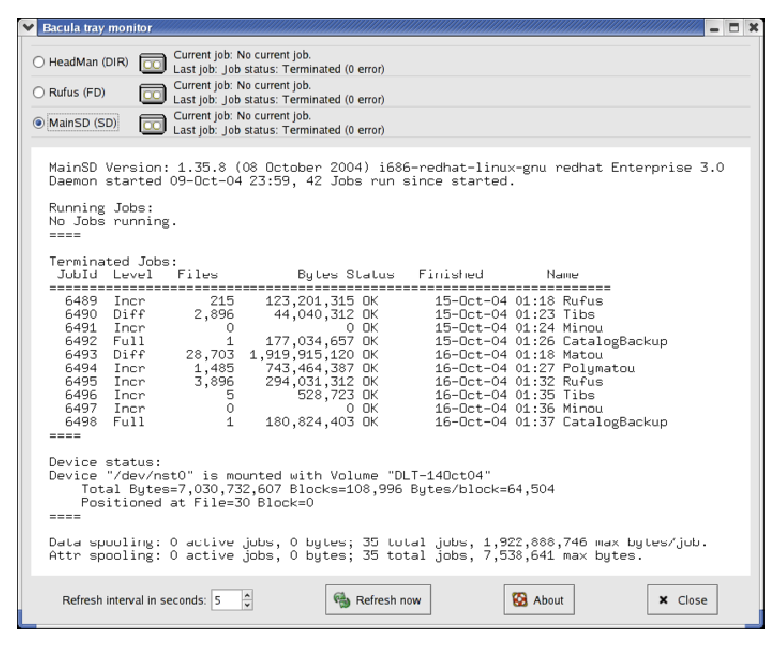
\includegraphics{./Bacula-tray-monitor.eps} 

L'image montre le tray-monitor configur\'e pour trois {\it daemons}. En
cliquant sur les boutons radio dans le coin en haut \`a gauche de l'image,
vous pouvez voir l'\'etat de chacun des {\it daemons}. L'image montre l'\'etat
du Storage Daemon (MainSD) s\'electionn\'e. 

Le fichier de configuration du Monitor se trouve dans le r\'epertoire
sp\'ecifi\'e au niveau de l'option {\bf \verb{--{sysconfdir} de la commande {\bf
./configure} et se nomme par d\'efaut {\bf tray-monitor.conf}. En principe,
pour les nouveaux utilisateurs, il suffit de changer les permissions de ce
fichier pour permettre aux utilisateurs non-root d'ex\'ecuter le Monitor, en
effet cette application doit \^etre ex\'ecut\'e par le m\^eme utilisateur que
l'environnement graphique (n'oubliez pas de donner aux non-root le droit
d'ex\'ecuter {\bf bacula-tray-monitor}). Ceci ne constitue pas une faille de
s\'ecurit\'e tant que vous utilisez les r\'eglages par d\'efaut. 

\subsection{
\ilink{Configurer le File Daemon}{_ChapterStart25}}
\index[general]{Configurer le File Daemon }
\index[general]{Daemon!Configurer le File }
\addcontentsline{toc}{subsection}{Configurer le File Daemon}

Le File Daemon, est le programme qui s'ex\'ecute sur chaque machine cliente. A
la demande du Director, il d\'etermine les fichiers \`a sauvegarder et les
exp\'edie au Storage Daemon. 

Le fichier de configuration du File Daemon se trouve dans le r\'epertoire
sp\'ecifi\'e au niveau de l'option {\bf \verb{--{sysconfdir} de la commande {\bf
./configure} et se nomme par d\'efaut {\bf bacula-fd.conf}. Normalement, pour
les nouveaux utilisateurs, aucune modification n'est requise pour ce fichier.
Les r\'eglages par d\'efaut sont raisonnables. Cependant, si vous envisagez de
sauvegarder plus d'une machine, il vous faudra installer le File Daemon avec
un fichier de configuration sp\'ecifique sur chaque machine \`a sauvegarder.
Les informations concernant chaque File Daemon doivent appara{\^\i}tre dans le
fichier de configuration du Director. 

\subsection{
\ilink{Configurer le Director}{_ChapterStart40}}
\index[general]{Director!Configurer le }
\index[general]{Configurer le Director }
\addcontentsline{toc}{subsection}{Configurer le Director}

Le director est le programme central qui contr\^ole tous les autres {\it
daemons}. Il planifie et surveille les jobs \`a ex\'ecuter. 

Le fichier de configuration du Director se trouve dans le r\'epertoire
sp\'ecifi\'e au niveau de l'option {\bf \verb{--{sysconfdir} de la commande {\bf
./configure} et se nomme par d\'efaut {\bf bacula-dir.conf}. 

En g\'en\'eral, la seule modification n\'ecessaire consiste \`a faire en sorte
que la directive {\bf Include} de la Ressource FileSet contienne au moins une
ligne avec un nom de fichier ou de r\'epertoire valide \`a sauvegarder. 

Si vous ne poss\'edez pas de lecteur DLT, vous voudrez probablement modifier
la ressource Storage pour donner un nom plus repr\'esentatif de votre
p\'eriph\'erique de stockage. Vous pouvez toujours utiliser les noms existants
puisque vous \^etes libre de les assigner arbitrairement, mais ils doivent
s'accorder avec les noms correspondants dans le fichier de configuration du
Storage Daemon. 

Vous pouvez aussi changer l'adresse \'electronique pour les notifications vers
votre propre adresse e-mail plut\^ot que vers celle de {\bf root}
(configuration par d\'efaut). 

Enfin, si vous avez plusieurs syst\`emes \`a sauvegarder, il vous faudra
sp\'ecifier un File Daemon (ou client) pour chaque syst\`eme sauvegard\'e,
pr\'ecisant ses nom, adresse et mot de passe. Nous estimons que baptiser vos
{\it daemons} du nom de vos syst\`emes suffix\'es avec {\bf -fd} aide beaucoup
\`a corriger les erreurs. Ainsi, si votre syst\`eme est {\bf foobaz}, vous
nommerez le {\it daemon} {\bf foobaz-fd}. Pour le Director, vous pourriez
utiliser {\bf foobaz-dir}, et {\bf foobaz-sd} pour le Storage Daemon. 
Chacun de vos composants de Bacula {\bf doit} avoir un nom unique 
Si vous les nommez tous \`a l'identique, en plus de ne jamais savoir 
quel {\it daemon} envoie quel message, s'ils partagent le m\^eme r\'epertoire 
de travail (working directory), les noms de fichiers temporaires des {\it daemons} 
ne seront pas uniques et vous aurez d'\'etranges erreurs.

\subsection{
\ilink{Configurer le Storage Daemon}{_ChapterStart31}}
\index[general]{Daemon!Configurer le Storage }
\index[general]{Configurer le Storage Daemon }
\addcontentsline{toc}{subsection}{Configurer le Storage Daemon}

Le Storage Daemon est responsable, sur demande du Director, de la r\'eception
des donn\'ees en provenance des File Daemons, et de leur \'ecriture sur le
medium de stockage, ou, dans le cas d'une restauration, de trouver les
donn\'ees pour les envoyer vers le File Daemon. 

Le fichier de configuration du Storage Daemon se trouve dans le r\'epertoire
sp\'ecifi\'e au niveau de l'option {\bf \verb{--{sysconfdir} de la commande {\bf
./configure} et se nomme par d\'efaut {\bf bacula-sd.conf}. Modifiez ce
fichier pour accorder les noms de p\'eriph\'eriques de stockage \`a ceux que
vous poss\'edez. Si le processus d'installation a convenablement d\'etect\'e
votre syst\`eme, elles seront d\'ej\`a correctement r\'egl\'ees. Ces
ressources de stockage "Name" et "Media Type" doivent \^etre les m\^emes
que leurs correspondantes du fichier de configuration du Director {\bf
bacula-dir.conf}. Si vous souhaitez sauvegarder vers un fichier plut\^ot que
sur des bandes, la ressource Device doit pointer vers un r\'epertoire o\`u des
fichiers seront cr\'e\'es en guise de Volumes lorque vous \'etiquetterez
(label) vos Volumes. 
\label{ConfigTesting}

\section{Tester vos Fichiers de Configuration}
\index[general]{Configuration!Tester vos Fichiers de }
\index[general]{Tester vos Fichiers de Configuration }
\addcontentsline{toc}{section}{Tester vos Fichiers de Configuration}

Vous pouvez tester la validit\'e syntaxique de vos fichiers de configuration,
afficher tout message d'erreur et terminer. Par exemple, en supposant que vous
avez install\'e vos binaires et fichiers de configuration dans le m\^eme
r\'epertoire, 

\footnotesize
\begin{verbatim}
cd <installation-directory>
./bacula-dir -t -c bacula-dir.conf
./bacula-fd -t -c bacula-fd.conf
./bacula-sd -t -c bacula-sd.conf
./bconsole -t -c bconsole.conf
./gnome-console -t -c gnome-console.conf
./bwx-console -t -c wx-console.conf
su <normal user> -c "./bacula-tray-monitor -t -c tray-monitor.conf"
\end{verbatim}
\normalsize

testera le fichier de configuration de chacun des principaux programmes. Si le
fichier de configuration est correct, le programme se termine
sans rien afficher. Veuillez noter que selon les options de configuration que
vous avez choisies, il se peut qu'aucune des commandes ci-dessus ne soit
valable sur votre syst\`eme. Si vous avez install\'e les binaires dans les
r\'epertoires traditionnels d'Unix plut\^ot que dans un simple r\'epertoire,
il vous faudra modifier les commandes ci-dessus en cons\'equence (pas de
"./" devant les commandes, et un chemin devant les fichiers de
configuration). 
\label{TapeTesting}

\section{Tester la compatibilit\'e de Bacula avec votre lecteur de bandes}
\index[general]{Tester la compatibilit\'e de Bacula avec votre lecteur de
bandes }
\index[general]{Bandes!Tester la compatibilit\'e de Bacula avec votre lecteur
de }
\addcontentsline{toc}{section}{Tester la compatibilit\'e de Bacula avec
votre lecteur de bandes}

Avant de gaspiller votre temps avec Bacula pour finalement constater qu'il ne
fonctionne pas avec votre lecteur de bandes, veuillez s'il vous pla\^it lire le
chapitre 
\ilink{btape -- Tester votre lecteur de bandes}{_ChapterStart27}
de ce manuel. Si vous poss\'edez un lecteur standard SCSI moderne sur un Linux
ou un Solaris, fort probablement, il fonctionnera, mais mieux vaut tester que
d'\^etre d\'e\c{c}u. Pour FreeBSD (et probablement les autres xBSD), la
lecture du chapitre mentionn\'e ci-dessus est un devoir. Pour FreeBSD,
consultez aussi 
\elink{The FreeBSD Diary}{http://www.freebsddiary.org/bacula.php} pour une
description d\'etaill\'ee de la m\'ethode pour faire fonctionner Bacula sur
votre syst\`eme. De plus, les utilisateurs de versions de FreeBSD
ant\'erieures \`a 4.9-STABLE dat\'ee du lundi 29 d\'ecembre 2003 15:18:01 UTC
qui pr\'evoient d'utiliser des lecteurs de bandes sont invit\'es \`a lire le
fichier {\bf platforms/freebsd/pthreads-fix.txt} du r\'epertoire principal de
Bacula, qui contient d'importantes informations sur la compatibilit\'e de
Bacula avec leur syst\`eme. 
\label{notls}

\section{D\'ebarrassez-vous du r\'epertoire /lib/tls}
\index[general]{D\'ebarrassez-vous du r\'epertoire /lib/tls }
\addcontentsline{toc}{section}{D\'ebarrassez-vous du r\'epertoire /lib/tls}

La nouvelle librairie pthreads {\bf /lib/tls} install\'ee par d\'efaut sur les
syst\`emes Red Hat r\'ecents (kernels 2.4.x) est d\'efectueuse. Vous devez la
supprimer ou la renommer, puis rebooter votre syst\`eme avant d'ex\'ecuter
Bacula, faute de quoi, apr\`es environ une semaine de fonctionnement, Bacula
se bloquera pour de longues p\'eriodes, voire d\'efinitivement. Veuillez consulter 
le chapitre \ilink{Syst\`emes support\'es}{SupportedOSes} pour plus
d'informations sur ce probl\`eme. 

Ce probl\`eme n'existe plus avec les noyaux 2.6.

\label{Running1}

\section{Ex\'ecuter Bacula}
\index[general]{Bacula!Ex\'ecuter }
\index[general]{Ex\'ecuter Bacula }
\addcontentsline{toc}{section}{Ex\'ecuter Bacula}

La partie la plus importante de l'ex\'ecution de Bacula est probablement la
capacit\'e de restaurer les fichiers. Si vous n'avez pas essay\'e de
r\'ecup\'erer des fichiers au moins une fois, vous subirez une bien plus forte
pression le jour o\`u vous devrez r\'eellement le faire, et serez enclin \`a
commettre des erreurs que vous n'auriez pas commises si vous aviez d\'ej\`a
essay\'e. 

Pour avoir rapidement une bonne id\'ee de la fa\c{c}on d'utiliser Bacula,
nous vous recommandons {\bf fortement} de suivre les exemples du 
\ilink{chapitre ex\'ecuter Bacula}{_ChapterStart1} de ce manuel,
o\`u vous trouverez des informations d\'etaill\'ees sur l'ex\'ecution de
Bacula. 

\section{Rotation des logs}
\index[general]{Logs!Rotation des }
\index[general]{Rotation des logs }
\addcontentsline{toc}{section}{Rotation des logs}

Si vous utilisez le {\bf bacula-dir.conf} par d\'efaut ou une variante, vous
constaterez qu'il r\'ecup\`ere toutes les sorties de Bacula dans un fichier.
Pour \'eviter que ce fichier ne croisse sans limites, nous vous recommandons
de copier le fichier {\bf logrotate} depuis {\bf scripts/logrotate} vers {\bf
/etc/logrotate.d/bacula}. Ainsi les fichiers de logs subiront une rotation
mensuelle et seront conserv\'es pour une dur\'ee maximum de cinq mois. Vous
pouvez \'editer ce fichier pour adapter la rotation \`a votre convenance. 

\section{Log Watch}
\index[general]{Watch!Log}
\index[general]{Log Watch}
\addcontentsline{toc}{section}{Log Watch}
Certains syst\`emes tels que RedHat et Fedora ex\'ecutent le programme 
logwatch chaque nuit pour analyser vos fichiers de log et vous 
envoyer un rapport par mail. Si vous souhaitez inclure la sortie 
de vos jobs Bacula dans ce rapport, veuillez regarder dans le r\'epertoire  
{\bf scripts/logwatch}. Le fichier {\bf README} fournit une br\`eve 
explication sur la fa\c {c}on d'installer le script, et quelle genre 
de r\'esultats en attendre.

\section{Reprise d'activit\'e apr\`es un d\'esastre (disaster recovery)}
\index[general]{Recovery!Reprise d'activit\'e apr\`es un d\'esastre disaster }
\index[general]{Reprise d'activit\'e apr\`es un d\'esastre (disaster recovery)
}
\addcontentsline{toc}{section}{Reprise d'activit\'e apr\`es un d\'esastre
(disaster recovery)}

Si vous avez l'intention d'utiliser Bacula en tant qu'outil de disaster
recovery plut\^ot que comme un simple programme pour restaurer les fichiers
perdus, vous serez int\'eress\'e par le 
\ilink{chapitre Plan de reprise d'activit\'e avec
Bacula}{_ChapterStart38} de ce manuel. 

De toute fa\c{c}on, vous \^etes fortement invit\'e \`a tester soigneusement
la restauration de quelques fichiers que vous aurez pr\'ealablement
sauvegard\'es, plut\^ot que d'attendre qu'un d\'esastre ne frappe. Ainsi, vous
serez pr\'epar\'e. 

%%
%%

\chapter{Installing Bacula}
\label{InstallChapter}
\index[general]{Bacula!Installing}
\index[general]{Installing Bacula}

In general, you will need the Bacula source release, and if you want to run
a Windows client, you will need the Bacula Windows binary release.
However, Bacula needs certain third party packages (such as {\bf MySQL},
{\bf PostgreSQL}, or {\bf SQLite} to build and run
properly depending on the
options you specify.  Normally, {\bf MySQL} and {\bf PostgreSQL} are
packages that can be installed on your distribution.  However, if you do
not have them, to simplify your task, we have combined a number of these
packages into three {\bf depkgs} releases (Dependency Packages).  This can
vastly simplify your life by providing you with all the necessary packages
rather than requiring you to find them on the Web, load them, and install
them.

\section{Source Release Files}
\index[general]{Source Files}
\index[general]{Release Files}
 Beginning with Bacula 1.38.0, the source code has been broken into
 four separate tar files each corresponding to a different module in
 the Bacula SVN. The released files are:

\begin{description}
\item [bacula-3.0.3.tar.gz]
  This is the primary source code release for Bacula. On each
  release the version number (3.0.3) will be updated.

\item [bacula-docs-3.0.3.tar.gz]
  This file contains a copy of the docs directory with the
  documents prebuild. English HTML directory, single HTML
  file, and pdf file. The French and German translations
  are in progress, but are not built.

\item [bacula-gui-3.0.3.tar.gz]
  This file contains the non-core GUI programs. Currently,
  it contains bacula-web, a PHP program for producing management
  viewing of your Bacula job status in a browser; and bimagemgr
  a browser program for burning CDROM images with Bacula Volumes.

\item [bacula-rescue-3.0.3.tar.gz]
  This is the Bacula Rescue CDROM code. Note, the version number
  of this package is not tied to the Bacula release version, so
  it will be different.  Using this code, you can burn a CDROM
  with your system configuration and containing a statically
  linked version of the File daemon. This can permit you to easily
  repartition and reformat your hard disks and reload your
  system with Bacula in the case of a hard disk failure.
  Unfortunately this rescue disk does not properly boot for
  all Linux distributions. The problem is that the boot procedure
  can vary significantly between distributions, and even within
  a distribution, they are a moving target.

  This package evolves slower than the Bacula source code,
  so there may not always be a new release of the rescue package when
  making minor updates to the Bacula code. For example, when releasing
  Bacula version 3.0.3, the rescue package may still be at a prior
  version if there were no updates.

\item [winbacula-3.0.3.exe]
  This file is the 32 bit Windows installer for installing
  the Windows client (File daemon) on a Windows machine.
  This client will also run on 64 bit Windows machines.
  Beginning with Bacula version 1.39.20, this executable will
  also optionally load the Win32 Director and the Win32 
  Storage daemon.

\item [win64bacula-3.0.3.exe]
  This file is the 64 bit Windows installer for installing
  the Windows client (File daemon) on a Windows machine.
  This client will only run on 64 bit Windows OS machines.
  It will not run on 32 bit machines or 32 bit Windows OSes.
  The win64bacula release is necessary for Volume Shadow
  Copy (VSS) to work on Win64 OSes.  This installer
  installs only the FD, the Director and Storage daemon
  are not included.

\end{description}

\label{upgrading1}
\section{Upgrading Bacula}
\index[general]{Bacula!Upgrading}
\index[general]{Upgrading Bacula}
\index[general]{Upgrading}

If you are upgrading from one Bacula version to another, you should first
carefully read the ReleaseNotes of all major versions between your current
version and the version to which you are upgrading.  In many upgrades,
especially for minor patch upgrades (e.g. between 3.0.0 and 3.0.1) there
will be no database upgrade, and hence the process is rather simple.

With version 3.0.0 and later, you {\bf must} ensure that on any one
machine that all components of Bacula are running on exactly the
same version.  Prior to version 3.0.0, it was possible to run a 
lower level FD with a newer Director and SD.  This is no longer the
case.  

As always, we attempt to support older File daemons. This avoids the
need to do a simultaneous upgrade of many machines. For exactly what
older versions of the FD are supported, please see the ReleaseNotes 
for the new version.  In any case, you must always upgrade both the
Director and the Storage daemon at the same time, and you must also
upgrade any File daemon that is running on the same machine as a Director
or a Storage daemon (see the prior paragraph).

If the Bacula catalog
database has been upgraded (as it is almost every major release), you will
either need to reinitialize your database starting from scratch (not
normally a good idea), or save an ASCII copy of your database, then proceed
to upgrade it. If you are upgrading two major versions (e.g. 1.36 to 2.0)
then life will be more complicated because you must do two database
upgrades. See below for more on this.

Upgrading the catalog is normally done after Bacula is build and installed
by:

\begin{verbatim}
cd <installed-scripts-dir> (default /etc/bacula)
./update_bacula_tables
\end{verbatim}

This update script can also be find in the Bacula source src/cats
directory.

If there are several database upgrades between your version and the
version to which you are upgrading, you will need to apply each database
upgrade script. For your convenience, you can find all the old upgrade scripts
in the {\bf upgradedb} directory of the source code. You will need to edit the
scripts to correspond to your system configuration. The final upgrade script,
if any, can be applied as noted above.

If you are upgrading from one major version to another, you will need to
replace all your components at the same time as generally the inter-daemon
protocol will change. However, within any particular release (e.g. version
1.32.x) unless there is an oversight or bug, the daemon protocol will not
change. If this is confusing, simply read the ReleaseNotes very carefully as
they will note if all daemons must be upgraded at the same time. 

Finally, please note that in general it is not necessary or desirable
to do a {\bf make uninstall} before doing an upgrade providing you are careful
not to change the installation directories. In fact, if you do so, you will 
most likely delete all your conf files, which could be disastrous.
The normal procedure during an upgrade is simply:

\begin{verbatim}
./configure (your options)
make
make install
\end{verbatim}

In general none of your existing .conf or .sql files will be overwritten,
and you must do both the {\bf make} and {\bf make install}  commands, a
{\bf make install} without the preceding {\bf make} will not work.
  
For additional information on upgrading, please see the \ilink{Upgrading Bacula
Versions}{upgrading} in the Tips chapter of this manual.

\section{Releases Numbering}
\index[general]{Release Numbering}
\index[general]{Version Numbering}
Every Bacula release whether beta or production has a different number  
as well as the date of the release build. The numbering system follows
traditional Open Source conventions in that it is of the form.

\begin{verbatim}
major.minor.release
\end{verbatim}

For example:
\begin{verbatim}
1.38.11
\end{verbatim}

where each component (major, minor, patch) is a number.
The major number is currently 1 and normally does not change
very frequently.  The minor number starts at 0 and increases
each for each production release by 2 (i.e. it is always an
even number for a production release), and the patch number is
starts at zero each time the minor number changes.  The patch
number is increased each time a bug fix (or fixes) is released
to production.

So, as of this date (10 September 2006), the current production Bacula
release is version 1.38.11.  If there are bug fixes, the next release
will be 1.38.12 (i.e. the patch number has increased by one).

For all patch releases where the minor version number does not change,
the database and all the daemons will be compatible.  That means that
you can safely run a 1.38.0 Director with a 1.38.11 Client.  Of course,
in this case, the Director may have bugs that are not fixed. Generally,
within a minor release (some minor releases are not so minor), all
patch numbers are officially released to production. This means that while
the current Bacula version is 1.38.11, versions 1.38.0, 1.38.1, ... 1.38.10
have all been previously released.

When the minor number is odd, it indicates that the package is under 
development and thus may not be stable. For example, while the current 
production release of Bacula is currently 1.38.11, the current development
version is 1.39.22. All patch versions of the development code are 
available in the SVN (source repository).  However, not all patch versions
of the development code (odd minor version) are officially released. When
they are released, they are released as beta versions (see below for a
definition of what beta means for Bacula releases).                     

In general when the minor number increases from one production release
to the next (i.e. 1.38.x to 1.40.0), the catalog database must be upgraded,
the Director and Storage daemon must always be on the same minor release
number, and often (not always), the Clients must also be on the same minor
release. As often as possible, we attempt to make new releases that are
downwards compatible with prior clients, but this is not always possible.
You must check the release notes.  In general, you will have fewer problems
if you always run all the components on the same minor version number (i.e.
all either 1.38.x or 1.40.x but not mixed).


\label{BetaReleases}
\section*{Beta Releases}
\index[general]{Beta Releases}
Towards the end of the development cycle, which typically runs
one year from a major release to another, there will be several beta
releases of the development code prior to a production release.  
As noted above, beta versions always have odd minor version numbers
(e.g 1.37.x or 1.39.x). 
The purpose of the beta releases is to allow early adopter users to test
the new code.  Beta releases are made with the following considerations:

\begin{itemize}
\item The code passes the regression testing on FreeBSD, Linux, and Solaris
  machines.

\item There are no known major bugs, or on the rare occasion that 
  there are, they will be documented or already in the bugs database.

\item Some of the new code/features may not yet be tested.

\item Bugs are expected to be found, especially in the new
  code before the final production release.

\item The code will have been run in production in at least one small
  site (mine).

\item The Win32 client will have been run in production at least
  one night at that small site.

\item The documentation in the manual is unlikely to be complete especially
  for the new features, and the Release Notes may not be fully
  organized.

\item Beta code is not generally recommended for everyone, but
  rather for early adopters.
\end{itemize}


\label{Dependency}
\section{Dependency Packages}
\index[general]{Dependency Packages}
\index[general]{Packages!Dependency}

As discussed above, we have combined a number of third party packages that
Bacula might need into the {\bf depkgs} release. You can,
of course, get the latest packages from the original authors or 
from your operating system supplier. The locations of
where we obtained the packages are in the README file in each package.
However, be aware that the packages in the depkgs files have been tested by us
for compatibility with Bacula. 

Typically, a dependency package will be named {\bf depkgs-ddMMMyy.tar.gz}
where {\bf dd} is the day we release it, {\bf MMM}
is the abbreviated month (e.g. Jan), and {\bf yy} is the year. An actual
example is: {\bf depkgs-24Jul09.tar.gz}. To install and build this package (if
needed), you do the following: 

\begin{enumerate}
\item Create a {\bf bacula} directory, into which you will place  both the
   Bacula source as well as the dependency package.  
\item Detar the {\bf depkgs} into the {\bf bacula} directory.  
\item cd bacula/depkgs  
\item make 
\end{enumerate}

Although the exact composition of the dependency packages may change from time
to time, the current makeup is the following: 

\addcontentsline{lot}{table}{Dependency Packages}
\begin{longtable}{|l|l|l|}
 \hline 
\multicolumn{1}{|c| }{\bf 3rd Party Package} & \multicolumn{1}{c| }{\bf depkgs}
     & \multicolumn{1}{c| }{\bf depkgs-qt} \\
 \hline {SQLite } & \multicolumn{1}{c| }{X } & \multicolumn{1}{c| }{ }\\
 \hline {SQLite3 } & \multicolumn{1}{c| }{X } & \multicolumn{1}{c| }{ }\\
 \hline {mtx } & \multicolumn{1}{c| }{X } & \multicolumn{1}{c| }{ } \\
 \hline {qt4 } & \multicolumn{1}{c| }{ } & \multicolumn{1}{c| }{X } \\
 \hline {qwt } & \multicolumn{1}{c| }{ } & \multicolumn{1}{c| }{X } \\
 \hline 
\end{longtable}

Note, some of these packages are quite large, so that building them can be a
bit time consuming. The above instructions will build all the packages
contained in the directory. However, when building Bacula, it will take only
those pieces that it actually needs. 

Alternatively, you can make just the packages that are needed. For example, 

\footnotesize
\begin{verbatim}
cd bacula/depkgs
make sqlite
\end{verbatim}
\normalsize

will configure and build only the SQLite package. 

You should build the packages that you will require in {\bf depkgs} a     
prior to configuring and building Bacula, since Bacula will need
them during the build process. 

For more information on the {\bf depkgs-qt} package, please read the
INSTALL file in the main directory of that package. If you are going to 
build Qt4 using {\bf depkgs-qt}, you must source the {\bf qt4-paths} file
included in the package prior to building Bacula. Please read the INSTALL
file for more details.

Even if you do not use SQLite, you might find it worthwhile to build {\bf mtx}
because the {\bf tapeinfo} program that comes with it can often provide you
with valuable information about your SCSI tape drive (e.g. compression,
min/max block sizes, ...). Note, most distros provide {\bf mtx} as part of 
their release.

The {\bf depkgs1} package is depreciated and previously contained
readline, which should be available on all operating systems.

The {\bf depkgs-win32} package is deprecated and no longer used in 
Bacula version 1.39.x and later. It was previously used to build
the native Win32 client program, but this program is now built on Linux
systems using cross-compiling.  All the tools and third party libraries
are automatically downloaded by executing the appropriate scripts.  See
src/win32/README.mingw32 for more details.

\section{Supported Operating Systems}
\label{Systems}
\index[general]{Systems!Supported Operating}
\index[general]{Supported Operating Systems}

Please see the 
\ilink{ Supported Operating Systems}{SupportedOSes} section
of the QuickStart chapter of this manual. 

\section{Building Bacula from Source}
\label{Building}
\index[general]{Source!Building Bacula from}
\index[general]{Building Bacula from Source}

The basic installation is rather simple. 

\begin{enumerate}
\item Install and build any {\bf depkgs} as noted above. This
   should be unnecessary on most modern Operating Systems.

\item Configure and install MySQL or PostgreSQL (if desired). 
   \ilink{Installing and Configuring MySQL Phase I}{MySqlChapter} or  
   \ilink{Installing and Configuring PostgreSQL Phase
   I}{PostgreSqlChapter}.  If you are installing from rpms, and are
   using MySQL, please be sure to install  {\bf mysql-devel}, so that the MySQL
   header files are available  while compiling Bacula. In addition, the MySQL
   client  library {\bf mysqlclient} requires the gzip compression library  {\bf
   libz.a} or {\bf libz.so}. If you are using rpm packages,  these libraries are
   in the {\bf libz-devel} package. On Debian  systems, you will need to load the
   {\bf zlib1g-dev} package. If  you are not using rpms or debs, you will need to
   find the  appropriate package for your system.  

   Note, if you already have a running MySQL or PostgreSQL on your system, you 
   can skip this phase provided that you have built the thread  safe libraries.
   And you have already installed the additional  rpms noted above.  

   SQLite is not supported on Solaris. This is because it
   frequently fails with bus errors.  However SQLite3 may work.

\item Detar the Bacula source code preferably into the {\bf bacula}  directory
   discussed above.  

\item {\bf cd} to the directory containing the source code.  

\item ./configure (with appropriate options as described below). Any
   path names you specify as options on the ./configure command line
   must be absolute paths and not relative.

\item Check the output of ./configure very carefully, especially  the Install
   binaries and Install config directories.  If they are not correct,
   please rerun ./configure until they  are. The output from ./configure is
   stored in {\bf config.out}  and can be re-displayed at any time without
   rerunning the  ./configure by doing {\bf cat config.out}.  

\item If after running ./configure once, you decide to change options  and
   re-run it, that is perfectly fine, but before re-running it,  you should run: 

\footnotesize
\begin{verbatim}
      make distclean
\end{verbatim}
\normalsize

so that you are sure to start from scratch and not have a  mixture of the two
options. This is because ./configure  caches much of the information. The {\bf
make distclean}  is also critical if you move the source directory from one 
machine to another. If the {\bf make distclean} fails,  just ignore it and
continue on.  

\item make  
   If you get errors while linking in the Storage daemon directory
   (src/stored), it is probably because you have not loaded the static
   libraries on your system.  I noticed this problem on a Solaris system.
   To correct it, make sure that you have not added {\bf
   {-}{-}enable-static-tools} to the {\bf ./configure} command.

   If you skip this step ({\bf make}) and proceed immediately to the {\bf
   make install} you are making two serious errors: 1.  your install will
   fail because Bacula requires a {\bf make} before a {\bf make install}.
   2.  you are depriving yourself of the chance to make sure there are no
   errors before beginning to write files to your system directories.
                                 

\item make install  
   Please be sure you have done a {\bf make} before entering this command,
   and that everything has properly compiled and linked without errors.


\item If you are new to Bacula, we {\bf strongly} recommend that you skip
   the next step and use the default configuration files, then run the
   example program in the next chapter, then come back and modify your
   configuration files to suit your particular needs.

\item Customize the configuration files for each of the three daemons 
   (Directory, File, Storage) and for the Console program.  For the details
   of how to do this, please see \ilink{Setting Up Bacula Configuration
   Files}{ConfigureChapter} in the Configuration chapter of this manual.  We
   recommend that you start by modifying the default configuration files
   supplied, making the minimum changes necessary.  Complete customization
   can be done after you have Bacula up and running.  Please take care when
   modifying passwords, which were randomly generated, and the {\bf Name}s
   as the passwords and names must agree between the configuration files
   for security reasons.  

\label{CreateDatabase}
\item Create the Bacula MySQL database and tables
   (if using MySQL)
      \ilink{Installing and Configuring MySQL Phase II}{mysql_phase2} or 
      create the Bacula PostgreSQL database and tables  
   \ilink{Configuring PostgreSQL
   II}{PostgreSQL_configure} or alternatively  if you are using
   SQLite \ilink{Installing and Configuring SQLite Phase II}{phase2}.  

\item Start Bacula ({\bf ./bacula start}) Note. the next chapter  shows you
   how to do this in detail.  

\item Interface with Bacula using the Console program  

\item For the previous two items, please follow the instructions  in the 
   \ilink{Running Bacula}{TutorialChapter} chapter of  this manual,
   where you will run a simple backup and do a  restore. Do this before you make
   heavy modifications to the  configuration files so that you are sure that
   Bacula works  and are familiar with it. After that changing the conf files 
   will be easier.  

\item If after installing Bacula, you decide to "move it", that is  to
   install it in a different set of directories, proceed  as follows:  

\footnotesize
\begin{verbatim}
      make uninstall
      make distclean
      ./configure (your-new-options)
      make
      make install
      
\end{verbatim}
\normalsize

\end{enumerate}

If all goes well, the {\bf ./configure} will correctly determine which
operating system you are running and configure the source code appropriately.
Currently, FreeBSD, Linux (Red Hat), and Solaris are supported. The Bacula
client (File daemon) is reported to work with MacOS X 10.3 is if 
readline support is not enabled (default) when building the client.       

If you install Bacula on more than one system, and they are identical, you can
simply transfer the source tree to that other system and do a "make
install". However, if there are differences in the libraries or OS versions,
or you wish to install on a different OS, you should start from the original
compress tar file. If you do transfer the source tree, and you have previously
done a ./configure command, you MUST do: 

\footnotesize
\begin{verbatim}
make distclean
\end{verbatim}
\normalsize

prior to doing your new ./configure. This is because the GNU autoconf tools
cache the configuration, and if you re-use a configuration for a Linux machine
on a Solaris, you can be sure your build will fail. To avoid this, as
mentioned above, either start from the tar file, or do a "make distclean". 

In general, you will probably want to supply a more complicated {\bf
configure} statement to ensure that the modules you want are built and that
everything is placed into the correct directories. 

For example, on Fedora, Red Hat, or SuSE one could use the following: 

\footnotesize
\begin{verbatim}
CFLAGS="-g -Wall" \
  ./configure \
    --sbindir=$HOME/bacula/bin \
    --sysconfdir=$HOME/bacula/bin \
    --with-pid-dir=$HOME/bacula/bin/working \
    --with-subsys-dir=$HOME/bacula/bin/working \
    --with-mysql \
    --with-working-dir=$HOME/bacula/bin/working \
    --with-dump-email=$USER
\end{verbatim}
\normalsize

The advantage of using the above configuration to start is that
everything will be put into a single directory, which you can later delete
once you have run the examples in the next chapter and learned how Bacula
works. In addition, the above can be installed and run as non-root. 

For the developer's convenience, I have added a {\bf defaultconfig} script to
the {\bf examples} directory. This script contains the statements that you
would normally use, and each developer/user may modify them to suit his needs.
You should find additional useful examples in this directory as well. 

The {\bf \verb:--:enable-conio} or {\bf \verb:--:enable-readline} options are useful because
they provide a command line history and editing capability for the Console
program. If you have included either option in the build, either the {\bf
termcap} or the {\bf ncurses} package will be needed to link. On most
systems, including Red Hat and SuSE, you should include the ncurses package.
If Bacula's configure process finds the ncurses libraries, it will use
those rather than the termcap library.
On some systems, such as SuSE, the termcap library is not in the standard
library directory.  As a consequence, the option may be disabled or you may
get an error message such as:

\footnotesize
\begin{verbatim}
/usr/lib/gcc-lib/i586-suse-linux/3.3.1/.../ld:
cannot find -ltermcap
collect2: ld returned 1 exit status
\end{verbatim}
\normalsize

while building the Bacula Console. In that case, you will need to set the {\bf
LDFLAGS} environment variable prior to building. 

\footnotesize
\begin{verbatim}
export LDFLAGS="-L/usr/lib/termcap"
\end{verbatim}
\normalsize

The same library requirements apply if you wish to use the readline
subroutines for command line editing and history or
if you are using a MySQL library that requires encryption. If you need encryption,
you can either export the appropriate additional library options as shown
above or, alternatively, you can include them directly on the ./configure line
as in: 

\footnotesize
\begin{verbatim}
LDFLAGS="-lssl -lcyrpto" \
   ./configure <your-options>
\end{verbatim}
\normalsize

On some systems such as Mandriva, readline tends to
gobble up prompts, which makes it totally useless. If this happens to you, use
the disable option, or if you are using version 1.33 and above try using {\bf
\verb:--:enable-conio} to use a built-in readline replacement. You will still need
either the termcap or the ncurses library, but it is unlikely that the {\bf conio}
package will gobble up prompts. 

readline is no longer supported after version 1.34.  The code within Bacula
remains, so it should be usable, and if users submit patches for it, we will
be happy to apply them.  However, due to the fact that each version of
readline seems to be incompatible with previous versions, and that there
are significant differences between systems, we can no longer afford to
support it.

\section{What Database to Use?}
\label{DB}
\index[general]{What Database to Use?}
\index[general]{Use!What Database to}

Before building Bacula you need to decide if you want to use SQLite, MySQL, or
PostgreSQL. If you are not already running MySQL or PostgreSQL, you might
want to start by testing with SQLite (not supported on Solaris).
This will greatly simplify the setup for you
because SQLite is compiled into Bacula an requires no administration. It
performs well and is suitable for small to medium sized installations (maximum
10-20 machines). However, we should note that a number of users have
had unexplained database corruption with SQLite. For that reason, we
recommend that you install either MySQL or PostgreSQL for production
work.

If you wish to use MySQL as the Bacula catalog, please see the 
\ilink{Installing and Configuring MySQL}{MySqlChapter} chapter of
this manual. You will need to install MySQL prior to continuing with the
configuration of Bacula. MySQL is a high quality database that is very
efficient and is suitable for any sized installation. It is slightly more
complicated than SQLite to setup and administer because it has a number of
sophisticated features such as userids and passwords. It runs as a separate
process, is truly professional and can manage a database of any size. 

If you wish to use PostgreSQL as the Bacula catalog, please see the 
\ilink{Installing and Configuring PostgreSQL}{PostgreSqlChapter}
chapter of this manual. You will need to install PostgreSQL prior to
continuing with the configuration of Bacula. PostgreSQL is very similar to
MySQL, though it tends to be slightly more SQL92 compliant and has many more
advanced features such as transactions, stored procedures, and the such. It
requires a certain knowledge to install and maintain. 

If you wish to use SQLite as the Bacula catalog, please see 
\ilink{Installing and Configuring SQLite}{SqlLiteChapter} chapter of
this manual. SQLite is not supported on Solaris.

\section{Quick Start}
\index[general]{Quick Start}
\index[general]{Start!Quick}

There are a number of options and important considerations given below
that you can skip for the moment if you have not had any problems building
Bacula with a simplified configuration as shown above. 
      
If the ./configure process is unable to find specific libraries (e.g.    
libintl, you should ensure that the appropriate package is installed on
your system. Alternatively, if the package is installed in a non-standard
location (as far as Bacula is concerned), then there is generally an
option listed below (or listed with "./configure {-}{-}help" that will
permit you to specify the directory that should be searched. In other
cases, there are options that will permit you to disable to feature 
(e.g. {-}{-}disable-nls).

If you want to dive right into it, we recommend you skip to the next chapter,
and run the example program. It will teach you a lot about Bacula and as an
example can be installed into a single directory (for easy removal) and run as
non-root. If you have any problems or when you want to do a real installation,
come back to this chapter and read the details presented below. 

\section{Configure Options}
\label{Options}
\index[general]{Options!Configure}
\index[general]{Configure Options}

The following command line options are available for {\bf configure} to
customize your installation. 

\begin{description}
\item [ {-}prefix=\lt{}patch\gt{}]
   \index[general]{{-}prefix}
   This option is meant to allow you to direct where the architecture
   independent files should be placed.  However, we find this a somewhat
   vague concept, and so we have not implemented this option other than
   what ./configure does by default.  As a consequence, we suggest that
   you avoid it. We have provided options that allow you to explicitly
   specify the directories for each of the major categories of installation
   files.
\item [ {-}{-}sbindir=\lt{}binary-path\gt{}]
   \index[general]{{-}{-}sbindir}
   Defines where the Bacula  binary (executable) files will be placed during a
   {\bf make  install} command.  

\item [ {-}{-}sysconfdir=\lt{}config-path\gt{}]
   \index[general]{{-}{-}sysconfdir}
   Defines where the Bacula configuration files should be placed during a
   {\bf make install} command.

\item [ {-}{-}mandir=\lt{}path\gt{}]
   \index[general]{{-}{-}mandir}
   Note, as of Bacula version 1.39.14, the meaning of any path
   specified on this option is change from prior versions. It
   now specifies the top level man directory.
   Previously the mandir specified the full path to where you
   wanted the man files installed.
   The man files will be installed in gzip'ed format under
   mandir/man1 and mandir/man8 as appropriate.
   For the install to succeed you must have {\bf gzip} installed
   on your system.

   By default, Bacula will install the Unix man pages in 
   /usr/share/man/man1 and /usr/share/man/man8.  
   If you wish the man page to be installed in
   a different location, use this option to specify the path.
   Note, the main HTML and PDF Bacula documents are in a separate
   tar file that is not part of the source distribution.

\item [ {-}{-}datadir=\lt{}path\gt{} ]
   \index[general]{{-}{-}datadir}
   If you translate Bacula or parts of Bacula into a different language
   you may specify the location of the po files using the {\bf
   {-}{-}datadir} option. You must manually install any po files as
   Bacula does not (yet) automatically do so.

\item [ {-}{-}disable-ipv6 ]
   \index[general]{{-}{-}disable-ipv6}

\item [ {-}{-}enable-smartalloc ]
   \index[general]{{-}{-}enable-smartalloc}
   This enables the inclusion of the Smartalloc orphaned buffer detection
   code.  This option is highly recommended.  Because we never build
   without this option, you may experience problems if it is not enabled.
   In this case, simply re-enable the option.  We strongly recommend
   keeping this option enabled as it helps detect memory leaks.  This
   configuration parameter is used while building Bacula

\item [ {-}{-}enable-bat ]
   \label{enablebat}
   \index[general]{{-}{-}enable-bat}
   If you have Qt4 >= 4.3 installed on your computer including the
   libqt4 and libqt4-devel (libqt4-dev on Debian) libraries, and you want
   to use the Bacula Administration Tool (bat) GUI Console interface to
   Bacula, you must specify this option.  Doing so will build everything in
   the {\bf src/qt-console} directory.  The build with enable-bat will work
   only with a full Bacula build (i.e. it will not work with a client-only
   build). 

   Qt4 is available on OpenSUSE 10.2, CentOS 5, Fedora, and Debian. If it
   is not available on your system, you can download the {\bf depkgs-qt}
   package from the Bacula Source Forge download area and build it and
   the qwt package, both of which are needed to build bat.  See the
   INSTALL file in that package for more details. In particular to use
   the Qt4 built by {\bf depkgs-qt} you {bf must} source the file
   {\bf qt4-paths}.

\item [ {-}{-}with-qwt=\lt{}path\gt{} ]
  \index[general]{{-}{-}with-qwt}
  The qwt package is a graphics library for Qt. If it is included
  during the building of bat, you will get one extra graphical function.
  At the current time, we recommend not including this option when
  building bat. The path specified must be an absolute path and
  not relative.  

  The qwt package is available for download from
  the qwt project on Source Forge.  If you wish, you may build and 
  install it on your system (by default in /usr/lib). 
  If you have done so, you would specify:

\begin{verbatim}
 --with-qwt=/usr/lib/qwt-5.0.2
\end{verbatim}

  Alternatively, you can download the Bacula depkgs-qt package (currently
  version 28Jul09) and build it, then assuming that you have put it 
  into a directory named bacula, you would specify:

\begin{verbatim}
 --with-qwt=$HOME/bacula/depkgs-qt/qwt
\end{verbatim}

   Some packages such as Debian do not adhere to the standard of
   naming the library libqwt.a or libqwt.so, and you will either need
   to manually add a soft link to the name they use or use the
   depkgs version, which handles the naming correctly.


\item [ {-}{-}enable-batch-insert ]
   \index[general]{{-}{-}enable-batch-insert}
   This option enables batch inserts of the attribute records (default) in
    the catalog database, which is much faster (10 times or more) than
   without this option for large numbers of files. However, this option
   will automatically be disabled if your SQL libraries are not
   thread safe. If you find that batch mode is not enabled on your Bacula
   installation, then your database most likely does not support threads.

   SQLite2 is not thread safe.  Batch insert cannot be enabled when using
   SQLite2

   On most systems, MySQL, PostgreSQL and SQLite3 are thread safe.

   To verify that your PostgreSQL is thread safe, you can try this
   (change the path to point to your particular installed libpq.a;
   these commands were issued on FreeBSD 6.2):

\begin{verbatim}
$ nm /usr/local/lib/libpq.a | grep PQputCopyData
00001b08 T PQputCopyData
$ nm /usr/local/lib/libpq.a | grep mutex
         U pthread_mutex_lock
         U pthread_mutex_unlock
         U pthread_mutex_init
         U pthread_mutex_lock
         U pthread_mutex_unlock
\end{verbatim}

   The above example shows a libpq that contains the required function
   PQputCopyData and is thread enabled (i.e. the pthread\_mutex* entries).
   If you do not see PQputCopyData, your version of PostgreSQL is too old
   to allow batch insert.  If you do not see the mutex entries, then thread
   support has not been enabled. Our tests indicate you usually need to
   change the configuration options and recompile/reinstall the PostgreSQL
   client software to get thread support.

   Bacula always links to the thread safe MySQL libraries.

   As a default, Bacula runs SQLite3 with {\bf PRAGMA synchronous=OFF}
   because it improves performance by more than 30 times. However, it 
   increases the possibility of a corrupted database. If you want more
   security, please modify src/version.h appropriately (it should be
   obvious when you look at the file).

   Running with Batch Insert turned on is recommended because it can
   significantly improve attribute insertion times. However, it does 
   put a significantly larger part of the work on your SQL engine, so
   you may need to pay more attention to tuning it. In particular,   
   Batch Insert can require large temporary table space, and consequently,
   the default location (often /tmp) may run out of space causing errors.
   For MySQL, the location is set in my.conf with "tmpdir".  You may also
   want to increase the memory available to your SQL engine to further
   improve performance during Batch Inserts.

\item [ {-}{-}enable-gnome ]
   \index[general]{{-}{-}enable-gnome}
   If you have GNOME installed on your computer including the
   GNOME development libraries, and you want to use the
   GNOME GUI Console interface to Bacula, you must specify this option.
   Doing so will build everything in the {\bf src/gnome2-console} directory.

\item [ {-}{-}enable-bwx-console ]
   \index[general]{{-}{-}enable-bwx-console}
   If you have wxWidgets installed on your computer and you want to use the
   wxWidgets GUI Console interface to Bacula, you must specify this option.
   Doing so will build everything in the {\bf src/wx-console} directory.
   This could also be useful to users who want a GUI Console and don't want
   to install GNOME, as wxWidgets can work with GTK+, Motif or even X11
   libraries.

\item [ {-}{-}enable-tray-monitor ]
   \index[general]{{-}{-}enable-tray-monitor}
   If you have GTK installed on your computer, you run a graphical
   environment or a window manager compatible with the FreeDesktop system
   tray standard (like KDE and GNOME) and you want to use a GUI to monitor
   Bacula daemons, you must specify this option.  Doing so will build
   everything in the {\bf src/tray-monitor} directory. Note, due to 
   restrictions on what can be linked with GPLed code, we were forced to
   remove the egg code that dealt with the tray icons and replace it by
   calls to the GTK+ API, and unfortunately, the tray icon API necessary
   was not implemented until GTK version 2.10 or later.

\item [ {-}{-}enable-static-tools]
   \index[general]{{-}{-}enable-static-tools}
   This option causes the linker to link the Storage daemon utility tools
   ({\bf bls}, {\bf bextract}, and {\bf bscan}) statically.  This permits
   using them without having the shared libraries loaded.  If you have
   problems linking in the {\bf src/stored} directory, make sure you have
   not enabled this option, or explicitly disable static linking by adding
   {\bf \verb:--:disable-static-tools}.

\item [ {-}{-}enable-static-fd]
   \index[general]{{-}{-}enable-static-fd}
   This option causes the make process to build a {\bf static-bacula-fd} in
   addition to the standard File daemon.  This static version will include
   statically linked libraries and is required for the Bare Metal recovery.
   This option is largely superseded by using {\bf make static-bacula-fd}
   from with in the {\bf src/filed} directory.  Also, the {\bf
   \verb:--:enable-client-only} option described below is useful for just
   building a client so that all the other parts of the program are not
   compiled.   
     
   When linking a static binary, the linker needs the static versions
   of all the libraries that are used, so frequently users will 
   experience linking errors when this option is used. The first 
   thing to do is to make sure you have the static glibc library 
   installed on your system. The second thing to do is the make sure
   you do not specify {\bf {-}{-}openssl} or {\bf {-}{-}with-python}
   on your ./configure statement as these options require additional
   libraries. You may be able to enable those options, but you will
   need to load additional static libraries.


\item [ {-}{-}enable-static-sd]
   \index[general]{{-}{-}enable-static-sd}
   This option causes the make process to build a {\bf static-bacula-sd} in
   addition to the standard Storage daemon.  This static version will
   include statically linked libraries and could be useful during a Bare
   Metal recovery.

   When linking a static binary, the linker needs the static versions
   of all the libraries that are used, so frequently users will 
   experience linking errors when this option is used. The first 
   thing to do is to make sure you have the static glibc library 
   installed on your system. The second thing to do is the make sure
   you do not specify {\bf {-}{-}openssl} or {\bf {-}{-}with-python}
   on your ./configure statement as these options require additional
   libraries. You may be able to enable those options, but you will
   need to load additional static libraries.


\item [ {-}{-}enable-static-dir]
   \index[general]{{-}{-}enable-static-dir}
   This option causes the make process to build a {\bf static-bacula-dir}
   in addition to the standard Director.  This static version will include
   statically linked libraries and could be useful during a Bare Metal
   recovery.

   When linking a static binary, the linker needs the static versions
   of all the libraries that are used, so frequently users will 
   experience linking errors when this option is used. The first 
   thing to do is to make sure you have the static glibc library 
   installed on your system. The second thing to do is the make sure
   you do not specify {\bf {-}{-}openssl} or {\bf {-}{-}with-python}
   on your ./configure statement as these options require additional
   libraries. You may be able to enable those options, but you will
   need to load additional static libraries.


\item [ {-}{-}enable-static-cons]
   \index[general]{{-}{-}enable-static-cons}
   This option causes the make process to build a {\bf static-console} and
   a {\bf static-gnome-console} in addition to the standard console.  This
   static version will include statically linked libraries and could be
   useful during a Bare Metal recovery.

   When linking a static binary, the linker needs the static versions
   of all the libraries that are used, so frequently users will 
   experience linking errors when this option is used. The first 
   thing to do is to make sure you have the static glibc library 
   installed on your system. The second thing to do is the make sure
   you do not specify {\bf {-}{-}openssl} or {\bf {-}{-}with-python}
   on your ./configure statement as these options require additional
   libraries. You may be able to enable those options, but you will
   need to load additional static libraries.


\item [ {-}{-}enable-client-only]
   \index[general]{{-}{-}enable-client-only}
   This option causes the make process to build only the File daemon and
   the libraries that it needs.  None of the other daemons, storage tools,
   nor the console will be built.  Likewise a {\bf make install} will then
   only install the File daemon.  To cause all daemons to be built, you
   will need to do a configuration without this option.  This option
   greatly facilitates building a Client on a client only machine.

   When linking a static binary, the linker needs the static versions
   of all the libraries that are used, so frequently users will 
   experience linking errors when this option is used. The first 
   thing to do is to make sure you have the static glibc library 
   installed on your system. The second thing to do is the make sure
   you do not specify {\bf {-}{-}openssl} or {\bf {-}{-}with-python}
   on your ./configure statement as these options require additional
   libraries. You may be able to enable those options, but you will
   need to load additional static libraries.

\item [ {-}{-}enable-build-dird]
   \index[general]{{-}{-}enable-build-dird}
   This option causes the make process to build the Director and the
   Director's tools. By default, this option is on, but you may turn
   it off by using {\bf {-}{-}disable-build-dird} to prevent the
   Director from being built.

\item [ {-}{-}enable-build-stored]
   \index[general]{{-}{-}enable-build-stored}
   This option causes the make process to build the Storage daemon.
   By default, this option is on, but you may turn
   it off by using {\bf {-}{-}disable-build-stored} to prevent the
   Storage daemon from being built.


\item [ {-}{-}enable-largefile]
   \index[general]{{-}{-}enable-largefile}
   This option (default) causes  Bacula to be built with 64 bit file address
   support if it  is available on your system. This permits Bacula to read and 
   write files greater than 2 GBytes in size. You may disable this  feature and
   revert to 32 bit file addresses by using  {\bf \verb:--:disable-largefile}.  

\item [ {-}{-}disable-nls]
   \index[general]{{-}{-}disable-nls}
   By default, Bacula uses the GNU Native Language Support (NLS) libraries. On
   some machines, these libraries may not be present or may not function 
   correctly (especially on non-Linux implementations). In such cases, you
   may specify {\bf {-}{-}disable-nls} to disable use of those libraries.
   In such a case, Bacula will revert to using English.

\item [ {-}{-}disable-ipv6 ]
   \index[general]{{-}{-}disable-ipv6}
   By default, Bacula enables IPv6 protocol. On some systems, the files
   for IPv6 may exist, but the functionality could be turned off in the
   kernel. In that case, in order to correctly build Bacula, you will
   explicitly need to use this option so that Bacula does not attempt
   to reference OS function calls that do not exist.

\item [ {-}{-}with-sqlite=\lt{}sqlite-path\gt{}]
   \index[general]{{-}{-}with-sqlite}
   This enables use of the SQLite version 2.8.x database.  The {\bf
   sqlite-path} is not normally specified as Bacula looks for the necessary
   components in a standard location ({\bf depkgs/sqlite}).  See
   \ilink{Installing and Configuring SQLite}{SqlLiteChapter} chapter of
    this manual for more details. SQLite is not supported on Solaris.

   See the note below under the {-}{-}with-postgresql item.

\item [ {-}{-}with-sqlite3=\lt{}sqlite3-path\gt{}]
   \index[general]{{-}{-}with-sqlite3}
   This enables use of the SQLite version 3.x database.  The {\bf
   sqlite3-path} is not normally specified as Bacula looks for the
   necessary components in a standard location ({\bf depkgs/sqlite3}).  See
   \ilink{Installing and Configuring SQLite}{SqlLiteChapter} chapter of
   this manual for more details. SQLite3 is not supported on Solaris.

\item [ {-}{-}with-mysql=\lt{}mysql-path\gt{}]
   \index[general]{{-}{-}with-mysql}
   This enables building of the Catalog services for Bacula.  It assumes
   that MySQL is running on your system, and expects it to be installed in
   the {\bf mysql-path} that you specify.  Normally, if MySQL is installed
   in a standard system location, you can simply use {\bf {-}{-}with-mysql}
   with no path specification.  If you do use this option, please proceed
   to installing MySQL in the \ilink{Installing and Configuring
   MySQL}{MySqlChapter} chapter before proceeding with the configuration.

   See the note below under the {-}{-}with-postgresql item.

\item [ {-}{-}with-postgresql=\lt{}path\gt{}]
   \index[general]{{-}{-}with-postgresql}
   This provides an explicit path to the PostgreSQL libraries if Bacula
   cannot find it by default.  Normally to build with PostgreSQL, you would
   simply use {\bf {-}{-}with-postgresql}.

   Note, for Bacula to be configured properly, you must specify one
   of the four database options supported.  That is:
   {-}{-}with-sqlite, {-}{-}with-sqlite3, {-}{-}with-mysql, or
   {-}{-}with-postgresql, otherwise the ./configure will fail.

\item [ {-}{-}with-openssl=\lt{}path\gt{}]
   This configuration option is necessary if you want to enable TLS (ssl),
   which encrypts the communications within       
   Bacula or if you want to use File Daemon PKI data encryption.
   Normally, the {\bf path} specification is not necessary since
   the configuration searches for the OpenSSL libraries in standard system
   locations. Enabling OpenSSL in Bacula permits secure communications
   between the daemons and/or data encryption in the File daemon.
   For more information on using TLS, please see the
   \ilink{Bacula TLS -- Communications Encryption}{CommEncryption} chapter
   of this manual.
   For more information on using PKI data encryption, please see the
   \ilink{Bacula PKI -- Data Encryption}{DataEncryption}
   chapter of this manual.

\item [ {-}{-}with-python=\lt{}path\gt{}]
   \index[general]{{-}{-}with-python}
   This option enables Bacula support for Python.  If no path is supplied,
   configure will search the standard library locations for Python 2.2,
   2.3, 2.4, or 2.5.  If it cannot find the library, you will need to
   supply a path to your Python library directory.  Please see the
   \ilink{Python chapter}{PythonChapter} for the details of using Python
   scripting.

\item [ {-}{-}with-libintl-prefix=\lt{}DIR\gt{}]
   \index[general]{{-}{-}with-libintl-prefix}
   This option may be used to tell Bacula to search DIR/include and
   DIR/lib for the libintl headers and libraries needed for Native
   Language Support (NLS).

\item [ {-}{-}enable-conio]
   \index[general]{{-}{-}enable-conio}
   Tells Bacula to enable building the small, light weight readline
   replacement routine.  It is generally much easier to configure than
   readline, although, like readline, it needs either the termcap or
   ncurses library.

\item [ {-}{-}with-readline=\lt{}readline-path\gt{}]
   \index[general]{{-}{-}with-readline}
   Tells Bacula where {\bf readline} is installed.  Normally, Bacula will
   find readline if it is in a standard library.  If it is not found and no
   {-}{-}with-readline is specified, readline will be disabled.  This
   option affects the Bacula build.  Readline provides the Console program
   with a command line history and editing capability and is no longer
   supported, so you are on your own if you have problems.

\item [ {-}{-}enable-readline]
   \index[general]{{-}{-}enable-readline}
   Tells Bacula to enable readline support.  It is normally disabled due to the
   large number of configuration  problems and the fact that the package seems to
   change in incompatible  ways from version to version.  

\item [ {-}{-}with-tcp-wrappers=\lt{}path\gt{}]
   \index[general]{{-}{-}with-tcp-wrappers}
   \index[general]{TCP Wrappers}
   \index[general]{Wrappers!TCP}
   \index[general]{libwrappers}
   This specifies that you  want TCP wrappers (man hosts\_access(5)) compiled in.
   The path is optional since  Bacula will normally find the libraries in the
   standard locations.  This option affects the Bacula build.  In specifying your
   restrictions in the {\bf /etc/hosts.allow}  or {\bf /etc/hosts.deny} files, do
   not use the {\bf twist}  option (hosts\_options(5)) or the Bacula process will
   be terminated. Note, when setting up your {\bf /etc/hosts.allow}
   or {\bf /etc/hosts.deny}, you must identify the Bacula daemon in
   question with the name you give it in your conf file rather than the
   name of the executable.
   
   For more information on configuring and testing TCP wrappers, please  see the 
   \ilink{Configuring and Testing TCP Wrappers}{wrappers}  section
   in the Security Chapter.  

   On SuSE, the libwrappers libraries needed to link Bacula are
   contained in the tcpd-devel package. On Red Hat, the package is named
   tcp\_wrappers.

\item [ {-}{-}with-archivedir=\lt{}path\gt{} ]
   \index[general]{{-}{-}with-archivedir}
   The directory used for disk-based backups.  Default value is /tmp.
   This parameter sets the default values in the bacula-dir.conf and bacula-sd.conf
   configuration files.  For example, it sets the Where directive for the
   default restore job and the Archive Device directive for the FileStorage
   device.

   This option is designed primarily for use in regression testing.
   Most users can safely ignore this option.

\item [ {-}{-}with-working-dir=\lt{}working-directory-path\gt{} ]
   \index[general]{{-}{-}with-working-dir}
   This option is mandatory and specifies a directory  into which Bacula may
   safely place files that  will remain between Bacula executions. For example, 
   if the internal database is used, Bacula will keep  those files in this
   directory.  This option is only used to modify the daemon  configuration
   files. You may also accomplish the same  thing by directly editing them later.
   The working directory  is not automatically created by the install process, so
   you  must ensure that it exists before using Bacula for the  first time. 

\item [ {-}{-}with-base-port=\lt{}port=number\gt{}]
   \index[general]{{-}{-}with-base-port}
   In order to run,  Bacula needs three TCP/IP ports (one for the Bacula 
   Console, one for the Storage daemon, and one for the File daemon).  The {\bf
   \verb:--:with-baseport} option will automatically assign three  ports beginning at
   the base port address specified. You may  also change the port number in the
   resulting configuration  files. However, you need to take care that the
   numbers  correspond correctly in each of the three daemon configuration 
   files. The default base port is 9101, which assigns ports 9101  through 9103.
   These ports (9101, 9102, and 9103) have been  officially assigned to Bacula by
   IANA.  This option is only used  to modify the daemon configuration files. You
   may also accomplish  the same thing by directly editing them later. 

\item [ {-}{-}with-dump-email=\lt{}email-address\gt{}]
   \index[general]{{-}{-}with-dump-email}
   This option specifies  the email address where any core dumps should be set.
   This option  is normally only used by developers.  

\item [ {-}{-}with-pid-dir=\lt{}PATH\gt{}  ]
   \index[general]{{-}{-}with-pid-dir}
   This specifies where Bacula should place the process id  file during
   execution. The default is: {\bf /var/run}.  This directory is not created by
   the install process, so  you must ensure that it exists before using Bacula
   the  first time.  

\item [ {-}{-}with-subsys-dir=\lt{}PATH\gt{}]
   \index[general]{{-}{-}with-subsys-dir}
   This specifies where Bacula should place the subsystem lock  file during
   execution. The default is {\bf /var/run/subsys}.  Please make sure that you do
   not specify the same directory  for this directory and for the {\bf sbindir}
   directory.  This directory is used only within the autostart scripts.  The
   subsys directory is not created by the Bacula install,  so you must be sure to
   create it before using Bacula. 

\item [ {-}{-}with-dir-password=\lt{}Password\gt{}]
   \index[general]{{-}{-}with-dir-password}
   This option allows you to specify the password used to  access the Director
   (normally from the Console program).  If it is not specified, configure will
   automatically create a random  password.  

\item [ {-}{-}with-fd-password=\lt{}Password\gt{} ]
   \index[general]{{-}{-}with-fd-password}
   This option allows you to specify the password used to  access the File daemon
   (normally called from the Director).  If it is not specified, configure will
   automatically create a random  password.  

\item [ {-}{-}with-sd-password=\lt{}Password\gt{} ]
   \index[general]{{-}{-}with-sd-password}
   This option allows you to specify the password used to access the Storage daemon
   (normally called from the Director).  If it is not specified, configure will
   automatically create a random  password.  

\item [ {-}{-}with-dir-user=\lt{}User\gt{} ]
   \index[general]{{-}{-}with-dir-user}
   This option allows you to specify the Userid used to run the Director.  The
   Director must be started as root, but doesn't need to run as root, and
   after doing preliminary initializations, it can "drop" to the UserId
   specified on this option.  
   If you specify this option, you must
   create the User prior to running {\bf make install}, because the
   working directory owner will be set to {\bf User}.
                       
\item [ {-}{-}with-dir-group=\lt{}Group\gt{} ]
   \index[general]{{-}{-}with-dir-group}
   This option allows you to specify the GroupId used to  run the Director. The
   Director must be started as root, but  doesn't need to run as root, and  after
   doing preliminary initializations, it can "drop"  to the GroupId specified
   on this option. 
   If you specify this option, you must
   create the Group prior to running {\bf make install}, because the
   working directory group will be set to {\bf Group}.

\item [ {-}{-}with-sd-user=\lt{}User\gt{} ]
   \index[general]{{-}{-}with-sd-user}
   This option allows you to specify the Userid used to  run the Storage daemon.
   The Storage daemon must be started as root, but  doesn't need to run as root,
   and  after doing preliminary initializations, it can "drop"  to the UserId
   specified on this option. If you use this option,  you will need to take care
   that the Storage daemon has access  to all the devices (tape drives, ...) that
   it needs. 

\item [ {-}{-}with-sd-group=\lt{}Group\gt{} ]
   \index[general]{{-}{-}with-sd-group}
   This option allows you to specify the GroupId used to  run the Storage daemon.
   The Storage daemon must be started as root, but  doesn't need to run as root,
   and  after doing preliminary initializations, it can "drop"  to the GroupId
   specified on this option. 

\item [ {-}{-}with-fd-user=\lt{}User\gt{} ]
   \index[general]{{-}{-}with-fd-user}
   This option allows you to specify the Userid used to  run the File daemon. The
   File daemon must be started as root,  and in most cases, it needs to run as
   root, so this option is  used only in very special cases,  after doing
   preliminary initializations, it can "drop"  to the UserId specified on this
   option. 

\item [ {-}{-}with-fd-group=\lt{}Group\gt{} ]
   \index[general]{{-}{-}with-fd-group}
   This option allows you to specify the GroupId used to  run the File daemon.
   The File daemon must be started as root, and  in most cases, it must be run as
   root, however,  after doing preliminary initializations, it can "drop"  to
   the GroupId specified on this option. 

\item [ {-}{-}with-mon-dir-password=\lt{}Password\gt{}]
   \index[general]{{-}{-}with-mon-dir-password}
   This option allows you to specify the password used to  access the Directory
   from the monitor.  If it is not specified, configure will
   automatically create a random  password.  

\item [ {-}{-}with-mon-fd-password=\lt{}Password\gt{} ]
   \index[general]{{-}{-}with-mon-fd-password}
   This option allows you to specify the password used to  access the File daemon
   from the Monitor.  If it is not specified, configure will
   automatically create a random  password.  

\item [ {-}{-}with-mon-sd-password=\lt{}Password\gt{} ]
   \index[general]{{-}{-}with-mon-sd-password}
   This option allows you to specify the password used to  access the
   Storage daemon from the Monitor. If it is not specified, configure will
   automatically create a random  password.  

\item [ {-}{-}with-db-name=\lt{}database-name\gt{} ]
   \index[general]{{-}{-}with-db-name}
   This option allows you to specify the database name to be used in
   the conf files.  The default is bacula.

\item [ {-}{-}with-db-user=\lt{}database-user\gt{} ]
   \index[general]{{-}{-}with-db-user}
   This option allows you to specify the database user name to be used in
   the conf files.  The default is bacula.

\end{description}

Note, many other options are presented when you do a {\bf ./configure
\verb:--:help}, but they are not implemented.

\section{Recommended Options for Most Systems}
\index[general]{Systems!Recommended Options for Most}
\index[general]{Recommended Options for Most Systems}

For most systems, we recommend starting with the following options: 

\footnotesize
\begin{verbatim}
./configure \
  --enable-smartalloc \
  --sbindir=$HOME/bacula/bin \
  --sysconfdir=$HOME/bacula/bin \
  --with-pid-dir=$HOME/bacula/bin/working \
  --with-subsys-dir=$HOME/bacula/bin/working \
  --with-mysql=$HOME/mysql \
  --with-working-dir=$HOME/bacula/working
\end{verbatim}
\normalsize

If you want to install Bacula in an installation directory rather than run it
out of the build directory (as developers will do most of the time), you
should also include the \verb:--:sbindir and \verb:--:sysconfdir options with appropriate
paths. Neither are necessary if you do not use "make install" as is the case
for most development work. The install process will create the sbindir and
sysconfdir if they do not exist, but it will not automatically create the
pid-dir, subsys-dir, or working-dir, so you must ensure that they exist before
running Bacula for the first time.

\section{Red Hat}
\index[general]{Red Hat}

Using SQLite: 

\footnotesize
\begin{verbatim}
 
CFLAGS="-g -Wall" ./configure \
  --sbindir=$HOME/bacula/bin \
  --sysconfdir=$HOME/bacula/bin \
  --enable-smartalloc \
  --with-sqlite=$HOME/bacula/depkgs/sqlite \
  --with-working-dir=$HOME/bacula/working \
  --with-pid-dir=$HOME/bacula/bin/working \
  --with-subsys-dir=$HOME/bacula/bin/working \
  --enable-bat \
  --with-qwt=$HOME/bacula/depkgs/qwt \
  --enable-conio
\end{verbatim}
\normalsize

or 

\footnotesize
\begin{verbatim}
 
CFLAGS="-g -Wall" ./configure \
  --sbindir=$HOME/bacula/bin \
  --sysconfdir=$HOME/bacula/bin \
  --enable-smartalloc \
  --with-mysql=$HOME/mysql \
  --with-working-dir=$HOME/bacula/working
  --with-pid-dir=$HOME/bacula/bin/working \
  --with-subsys-dir=$HOME/bacula/bin/working
  --enable-gnome \
  --enable-conio
\end{verbatim}
\normalsize

or finally, a completely traditional Red Hat Linux install: 

\footnotesize
\begin{verbatim}
CFLAGS="-g -Wall" ./configure \
  --sbindir=/usr/sbin \
  --sysconfdir=/etc/bacula \
  --with-scriptdir=/etc/bacula \
  --enable-smartalloc \
  --enable-bat \
  --with-qwt=$HOME/bacula/depkgs/qwt \
  --with-mysql \
  --with-working-dir=/var/bacula \
  --with-pid-dir=/var/run \
  --enable-conio
\end{verbatim}
\normalsize

Note, Bacula assumes that /var/bacula, /var/run, and /var/lock/subsys exist so
it will not automatically create them during the install process. 

\section{Solaris}
\index[general]{Solaris}

To build Bacula from source, you will need the following installed on your
system (they are not by default): libiconv, gcc 3.3.2, stdc++, libgcc (for
stdc++ and gcc\_s libraries), make 3.8 or later. 

You will probably also need to: Add /usr/local/bin to PATH and Add
/usr/ccs/bin to PATH for ar. 

It is possible to build Bacula on Solaris with the Solaris compiler, but
we recommend using GNU C++ if possible.  

A typical configuration command might look like:

\footnotesize
\begin{verbatim}
#!/bin/sh
CFLAGS="-g" ./configure \
  --sbindir=$HOME/bacula/bin \
  --sysconfdir=$HOME/bacula/bin \
  --with-mysql=$HOME/mysql \
  --enable-smartalloc \
  --with-pid-dir=$HOME/bacula/bin/working \
  --with-subsys-dir=$HOME/bacula/bin/working \
  --with-working-dir=$HOME/bacula/working
\end{verbatim}
\normalsize

As mentioned above, the install process will create the sbindir and sysconfdir
if they do not exist, but it will not automatically create the pid-dir,
subsys-dir, or working-dir, so you must ensure that they exist before running
Bacula for the first time.

Note, you may need to install the following packages to build Bacula
from source:
\footnotesize
\begin{verbatim}
SUNWbinutils,
SUNWarc,
SUNWhea,
SUNWGcc,
SUNWGnutls
SUNWGnutls-devel
SUNWGmake
SUNWgccruntime
SUNWlibgcrypt
SUNWzlib
SUNWzlibs
SUNWbinutilsS
SUNWGmakeS
SUNWlibm

export 
PATH=/usr/bin::/usr/ccs/bin:/etc:/usr/openwin/bin:/usr/local/bin:/usr/sfw/bin:/opt/sfw/bin:/usr/ucb:/usr/sbin
\end{verbatim}
\normalsize

If you have installed special software not normally in the Solaris
libraries, such as OpenSSL, or the packages shown above, then you may need
to add {\bf /usr/sfw/lib} to the library search path.  Probably the
simplest way to do so is to run:

\footnotesize
\begin{verbatim}
setenv LDFLAGS "-L/usr/sfw/lib -R/usr/sfw/lib"
\end{verbatim}
\normalsize

Prior to running the ./configure command.

Alternatively, you can set the LD\_LIBARY\_PATH and/or the LD\_RUN\_PATH
environment variables appropriately.

It is also possible to use the {\bf crle} program to set the library
search path.  However, this should be used with caution.

\section{FreeBSD}
\index[general]{FreeBSD}

Please see: 
\elink{The FreeBSD Diary}{http://www.freebsddiary.org/bacula.php} for a
detailed description on how to make Bacula work on your system. In addition,
users of FreeBSD prior to 4.9-STABLE dated Mon Dec 29 15:18:01 2003 UTC who
plan to use tape devices, please see the 
\ilink{Tape Testing Chapter}{FreeBSDTapes} of this manual for
{\bf important} information on how to configure your tape drive for
compatibility with Bacula. 

If you are using Bacula with MySQL, you should take care to compile MySQL with
FreeBSD native threads rather than LinuxThreads, since Bacula is normally built
with FreeBSD native threads rather than LinuxTreads. Mixing the two will
probably not work. 

\section{Win32}
\index[general]{Win32}

To install the binary Win32 version of the File daemon please see the 
\ilink{Win32 Installation Chapter}{Win32Chapter} in this document. 

\section{One File Configure Script}
\index[general]{Script!One File Configure}
\index[general]{One Files Configure Script}

The following script could be used if you want to put everything
in a single file:

\footnotesize
\begin{verbatim}
#!/bin/sh
CFLAGS="-g -Wall" \
  ./configure \
    --sbindir=$HOME/bacula/bin \
    --sysconfdir=$HOME/bacula/bin \
    --mandir=$HOME/bacula/bin \
    --enable-smartalloc \
    --enable-gnome \
    --enable-bat \
    --with-qwt=$HOME/bacula/depkgs/qwt \
    --enable-bwx-console \
    --enable-tray-monitor \
    --with-pid-dir=$HOME/bacula/bin/working \
    --with-subsys-dir=$HOME/bacula/bin/working \
    --with-mysql \
    --with-working-dir=$HOME/bacula/bin/working \
    --with-dump-email=$USER@your-site.com \
    --with-job-email=$USER@your-site.com \
    --with-smtp-host=mail.your-site.com
exit 0
\end{verbatim}
\normalsize

You may also want to put the following entries in your {\bf /etc/services}
file as it will make viewing the connections made by Bacula easier to
recognize (i.e. netstat -a): 

\footnotesize
\begin{verbatim}
bacula-dir      9101/tcp
bacula-fd       9102/tcp
bacula-sd       9103/tcp
\end{verbatim}
\normalsize

\section{Installing Bacula}
\index[general]{Bacula!Installing}
\index[general]{Installing Bacula}

Before setting up your configuration files, you will want to install Bacula in
its final location. Simply enter: 

\footnotesize
\begin{verbatim}
make install
\end{verbatim}
\normalsize

If you have previously installed Bacula, the old binaries will be overwritten,
but the old configuration files will remain unchanged, and the "new"
configuration files will be appended with a {\bf .new}. Generally if you have
previously installed and run Bacula you will want to discard or ignore the
configuration files with the appended {\bf .new}. 

\section{Building a File Daemon or Client}
\index[general]{Client!Building a File Daemon or}
\index[general]{Building a File Daemon or Client}

If you run the Director and the Storage daemon on one machine and you wish to
back up another machine, you must have a copy of the File daemon for that
machine. If the machine and the Operating System are identical, you can simply
copy the Bacula File daemon binary file {\bf bacula-fd} as well as its
configuration file {\bf bacula-fd.conf} then modify the name and password in
the conf file to be unique. Be sure to make corresponding additions to the
Director's configuration file ({\bf bacula-dir.conf}). 

If the architecture or the OS level are different, you will need to build a
File daemon on the Client machine. To do so, you can use the same {\bf
./configure} command as you did for your main program, starting either from a
fresh copy of the source tree, or using {\bf make\ distclean} before the {\bf
./configure}. 

Since the File daemon does not access the Catalog database, you can remove
the {\bf \verb:--:with-mysql} or {\bf \verb:--:with-sqlite} options, then
add {\bf \verb:--:enable-client-only}.  This will compile only the
necessary libraries and the client programs and thus avoids the necessity
of installing one or another of those database programs to build the File
daemon.  With the above option, you simply enter {\bf make} and just the
client will be built.

\label{autostart}
\section{Auto Starting the Daemons}
\index[general]{Daemons!Auto Starting the}
\index[general]{Auto Starting the Daemons}

If you wish the daemons to be automatically started and stopped when your
system is booted (a good idea), one more step is necessary. First, the
./configure process must recognize your system -- that is it must be a
supported platform and not {\bf unknown}, then you must install the platform
dependent files by doing: 

\footnotesize
\begin{verbatim}
(become root)
make install-autostart
\end{verbatim}
\normalsize

Please note, that the auto-start feature is implemented only on systems
that we officially support (currently, FreeBSD, Red Hat/Fedora Linux, and
Solaris), and has only been fully tested on Fedora Linux.

The {\bf make install-autostart} will cause the appropriate startup scripts
to be installed with the necessary symbolic links.  On Red Hat/Fedora Linux
systems, these scripts reside in {\bf /etc/rc.d/init.d/bacula-dir} {\bf
/etc/rc.d/init.d/bacula-fd}, and {\bf /etc/rc.d/init.d/bacula-sd}.  However
the exact location depends on what operating system you are using.

If you only wish to install the File daemon, you may do so with: 

\footnotesize
\begin{verbatim}
make install-autostart-fd
\end{verbatim}
\normalsize

\section{Other Make Notes}
\index[general]{Notes!Other Make}
\index[general]{Other Make Notes}

To simply build a new executable in any directory, enter: 

\footnotesize
\begin{verbatim}
make
\end{verbatim}
\normalsize

To clean out all the objects and binaries (including the files named 1, 2, or
3, which are development temporary files), enter: 

\footnotesize
\begin{verbatim}
make clean
\end{verbatim}
\normalsize

To really clean out everything for distribution, enter: 

\footnotesize
\begin{verbatim}
make distclean
\end{verbatim}
\normalsize

note, this cleans out the Makefiles and is normally done from the top level
directory to prepare for distribution of the source. To recover from this
state, you must redo the {\bf ./configure} in the top level directory, since
all the Makefiles will be deleted. 

To add a new file in a subdirectory, edit the Makefile.in in that directory,
then simply do a {\bf make}. In most cases, the make will rebuild the Makefile
from the new Makefile.in. In some case, you may need to issue the {\bf make} a
second time. In extreme cases, cd to the top level directory and enter: {\bf
make Makefiles}. 

To add dependencies: 

\footnotesize
\begin{verbatim}
make depend
\end{verbatim}
\normalsize

The {\bf make depend} appends the header file dependencies for each of the
object files to Makefile and Makefile.in. This command should be done in each
directory where you change the dependencies. Normally, it only needs to be run
when you add or delete source or header files. {\bf make depend} is normally
automatically invoked during the configuration process. 

To install: 

\footnotesize
\begin{verbatim}
make install
\end{verbatim}
\normalsize

This not normally done if you are developing Bacula, but is used if you are
going to run it to backup your system. 

After doing a {\bf make install} the following files will be installed on your
system (more or less). The exact files and location (directory) for each file
depends on your {\bf ./configure} command (e.g. bgnome-console and
bgnome-console.conf are not installed if you do not configure GNOME. Also, if
you are using SQLite instead of MySQL, some of the files will be different). 

NOTE: it is quite probable that this list is out of date.  But it is a
starting point.

\footnotesize
\begin{verbatim}
bacula
bacula-dir
bacula-dir.conf
bacula-fd
bacula-fd.conf
bacula-sd
bacula-sd.conf
bacula-tray-monitor
tray-monitor.conf
bextract
bls
bscan
btape
btraceback
btraceback.gdb
bconsole
bconsole.conf
create_mysql_database
dbcheck
delete_catalog_backup
drop_bacula_tables
drop_mysql_tables
bgnome-console
bgnome-console.conf
make_bacula_tables
make_catalog_backup
make_mysql_tables
mtx-changer
query.sql
bsmtp
startmysql
stopmysql
bwx-console
bwx-console.conf
9 man pages
\end{verbatim}
\normalsize

\label{monitor}

\section{Installing Tray Monitor}
\index[general]{Monitor!Installing Tray}
\index[general]{Installing Tray Monitor}

The Tray Monitor is already installed if you used the {\bf
\verb:--:enable-tray-monitor} configure option and ran {\bf make install}.

As you don't run your graphical environment as root (if you do, you should
change that bad habit), don't forget to allow your user to read {\bf
tray-monitor.conf}, and to execute {\bf bacula-tray-monitor} (this is not a
security issue).

Then log into your graphical environment (KDE, GNOME or something else), run
{\bf bacula-tray-monitor} as your user, and see if a cassette icon appears
somewhere on the screen, usually on the task bar.
If it doesn't, follow the instructions below related to your environment or
window manager. 

\subsection{GNOME}
\index[general]{GNOME}

System tray, or notification area if you use the GNOME terminology, has been
supported in GNOME since version 2.2. To activate it, right-click on one of
your panels, open the menu {\bf Add to this Panel}, then {\bf Utility} and
finally click on {\bf Notification Area}. 

\subsection{KDE}
\index[general]{KDE}

System tray has been supported in KDE since version 3.1. To activate it,
right-click on one of your panels, open the menu {\bf Add}, then {\bf Applet}
and finally click on {\bf System Tray}. 

\subsection{Other window managers}
\index[general]{Managers!Other window}
\index[general]{Other window managers}

Read the documentation to know if the Freedesktop system tray standard is
supported by your window manager, and if applicable, how to activate it. 

\section{Modifying the Bacula Configuration Files}
\index[general]{Modifying the Bacula Configuration Files}
\index[general]{Files!Modifying the Bacula Configuration}

See the chapter 
\ilink{Configuring Bacula}{ConfigureChapter} in this manual for
instructions on how to set Bacula configuration files. 

%%
%%

\chapter{Critical Items to Implement Before Production}
\label{CriticalChapter}
\index[general]{Production!Critical Items to Implement Before}
\index[general]{Critical Items to Implement Before Production}

We recommend you take your time before implementing a production on a Bareos
backup system since Bareos is a rather complex program, and if you make a
mistake, you may suddenly find that you cannot restore your files in case
of a disaster.  This is especially true if you have not previously used a
major backup product.

If you follow the instructions in this chapter, you will have covered most of
the major problems that can occur. It goes without saying that if you ever
find that we have left out an important point, please inform us, so
that we can document it to the benefit of everyone.

\label{Critical}
\section{Critical Items}
\index[general]{Critical Items}

The following assumes that you have installed Bareos, you more or less
understand it, you have at least worked through the tutorial or have
equivalent experience, and that you have set up a basic production
configuration. If you haven't done the above, please do so and then come back
here. The following is a sort of checklist that points with perhaps a brief
explanation of why you should do it.  In most cases, you will find the
details elsewhere in the manual.  The order is more or less the order you
would use in setting up a production system (if you already are in
production, use the checklist anyway).

\begin{itemize}
\item Test your tape drive for compatibility with Bareos by using the test
   command of the \ilink{btape}{btape} program.
% TODO: missing chapter
% \item Better than doing the above is to walk through the nine steps in the
%    \ilink{Tape Testing}{TapeTestingChapter} chapter of the manual. It
%    may take you a bit of time, but it will eliminate surprises.
\item Test the end of tape handling of your tape drive by using the
   fill command in the \ilink{btape}{btape} program.
\item Do at least one restore of files. If you backup multiple OS types
   (Linux, Solaris, HP, MacOS, FreeBSD, Win32, ...),
   restore files from each system type. The
   \ilink{Restoring Files}{RestoreChapter} chapter shows you how.
\item Write a bootstrap file to a separate system for each backup job.
   See \linkResourceDirective{Dir}{Job}{Write Bootstrap} directive and more details are available in the
   \nameref{BootstrapChapter} chapter. Also, the default
   \file{bareos-dir.conf} comes with a Write Bootstrap directive defined. This  allows
   you to recover the state of your system as of the last backup.
\item Backup your catalog. An example of this is found in the default
   bareos-dir.conf file. The backup script is installed by default and
   should handle any database, though you may want to make your own local
   modifications.  See also \ilink{Backing Up Your Bareos Database}{BackingUpBareos} for more
   information.
\item Write a bootstrap file for the catalog. An example of this is found in
   the default bareos-dir.conf file. This will allow you to quickly restore your
   catalog in the event it is wiped out -- otherwise it  is many excruciating
   hours of work.
\item Make a copy of the bareos-dir.conf, bareos-sd.conf, and
   bareos-fd.conf files that you are using on your server. Put it in a safe
   place (on another machine) as these files can be difficult to
   reconstruct if your server dies.
% \item Make a Bareos Rescue CDROM! See the
%    \ilink{Disaster Recovery Using a Bareos Rescue
%    CDROM}{RescueChapter} chapter. It is trivial to  make such a CDROM,
%    and it can make system recovery in the event of  a lost hard disk infinitely
%    easier.
\item Bareos assumes all filenames are in UTF-8 format. This is important
   when saving the filenames to the catalog. For Win32 machine, Bareos will
   automatically convert from Unicode to UTF-8, but on Unix, Linux, *BSD,
   and MacOS X machines, you must explicitly ensure that your locale is set
   properly. Typically this means that the {\bf LANG} environment variable
   must end in {\bf .UTF-8}. A full example is {\bf en\_US.UTF-8}. The
   exact syntax may vary a bit from OS to OS, and exactly how you define it
   will also vary.

   On most modern Win32 machines, you can edit the conf files with {\bf
   notepad} and choose output encoding UTF-8.
\end{itemize}

\section{Recommended Items}
\index[general]{Recommended Items}

Although these items may not be critical, they are recommended and will help
you avoid problems.

\begin{itemize}
\item Read the \nameref{QuickStartChapter} chapter
\item After installing and experimenting with Bareos, read and work carefully
   through the examples in the
   \nameref{TutorialChapter} chapter  of this manual.
\item Learn what each of the \nameref{sec:Utilities}
   does.
\item Set up reasonable retention periods so that your catalog does not  grow
   to be too big. See the following three chapters:\\
   \nameref{RecyclingChapter},\\
   \nameref{DiskChapter},\\
   \nameref{PoolsChapter}.
% \item Perform a bare metal recovery using the Bareos Rescue CDROM.  See the
%    \ilink{Disaster Recovery Using a Bareos Rescue CDROM}{RescueChapter}
%     chapter.
\end{itemize}

If you absolutely must implement a system where you write a different
tape each night and take it offsite in the morning. We recommend that you do
several things:
\begin{itemize}
\item Write a bootstrap file of your backed up data and a bootstrap file
   of your catalog backup to a external media like CDROM or USB stick, and take that with
   the tape.  If this is not possible, try to write those files to another
   computer or offsite computer, or send them as email to a friend. If none
   of that is possible, at least print the bootstrap files and take that
   offsite with the tape.  Having the bootstrap files will make recovery
   much easier.
\item It is better not to force Bareos to load a particular tape each day.
   Instead, let Bareos choose the tape.  If you need to know what tape to
   mount, you can print a list of recycled and appendable tapes daily, and
   select any tape from that list.  Bareos may propose a particular tape
   for use that it considers optimal, but it will accept any valid tape
   from the correct pool.
\end{itemize}

\chapter{Customizing the Configuration}
\label{ConfigureChapter}
\index[general]{Customizing the Configuration}

Each Bareos component (Director, Client, Storage, Console) has its own configuration
containing a set of resource definitions. These resources are very
similar from one service to another, but may contain different directives
(records) depending on the component. For example, in the Director configuration,
the \nameref{DirectorResourceDirector} defines the name of the Director, a number
of global Director parameters and his password. In the File daemon
configuration, the \nameref{ClientResourceDirector} specifies which Directors are
permitted to use the File daemon.

If you install all Bareos daemons (Director, Storage and File Daemon) onto one system,
the Bareos package tries its best to generate a working configuration as a basis for your individual configuration.

The details of each resource and the directives permitted therein are
described in the following chapters.

The following configuration files must be present:

\begin{itemize}
\item
   \nameref{DirectorChapter} -- to define the resources
   necessary for the Director. You define all the Clients  and Storage daemons
   that you use in this configuration file.
\item
   \nameref{StoredConfChapter} -- to define the resources to
   be used by each Storage daemon. Normally, you will have a single Storage
   daemon that controls your disk storage or tape drives. However, if you have
   tape drives on several machines, you will have at least one Storage daemon
   per machine.
\item
   \nameref{FiledConfChapter} -- to define the resources for
   each client to be backed up. That is, you will have a separate  Client
   resource file on each machine that runs a File daemon.
\item
   \nameref{ConsoleConfChapter} -- to define the resources for
   the Console program (user interface to the Director).  It defines which
Directors are  available so that you may interact with them.
\end{itemize}


\section{Configuration Path Layout}
\index[general]{Configuration!Directories}
\index[general]{Configuration!Subdirectories}

When a Bareos component starts, it reads its configuration.
In Bareos $<$ 16.2.2 only configuration files (which optionally can include other files) are supported.
Since Bareos \sinceVersion{}{Configuration Subdirectories}{16.2.2} also configuration subdirectories are supported.

\subsubsection{Naming}

In this section, the following naming is used:

\begin{itemize}
    \item \path|$CONFIGDIR|\hide{$} refers to the base configuration directory.
        Bareos Linux packages use \configPathUnix.
    \item A component is one of the following Bareos programs:
    \begin{itemize}
        \item bareos-dir
        \item bareos-sd
        \item bareos-fd
        \item bareos-traymonitor
        \item bconsole
        \item bat (only legacy config file: bat.conf)
        \item Bareos tools, like \nameref{sec:VolumeUtilityCommands} and others.
    \end{itemize}
    \item \path|$COMPONENT|\hide{$} refers to one of the listed components.
%
%     \item Legacy config file (still fully supported, with some
%           limitation when using the configuration API):
%         \begin{itemize}
%             \item \path|$CONFIGDIR/$COMPONENT.conf|
%         \end{itemize}
\end{itemize}

\subsection{What configuration will be used?}
\label{sec:ConfigurationFileOrConfigurationSubDirectories}

When starting a Bareos component, it will look for its configuration.
Bareos components allow the configuration file/directory to be specified as a command line parameter \path|-c $PATH|\hide{$}.

\begin{itemize}
    \item configuration path parameter is not given (default)
        \begin{itemize}
        \item \path|$CONFIGDIR/$COMPONENT.conf| is a file
            \begin{itemize}
            \item the configuration is read from the file \path|$CONFIGDIR/$COMPONENT.conf|
            \end{itemize}
        \item \path|$CONFIGDIR/$COMPONENT.d/| is a directory
            \begin{itemize}
            \item the configuration is read from \path|$CONFIGDIR/$COMPONENT.d/*/*.conf| (subdirectory configuration)
            \end{itemize}
        \end{itemize}
    \item configuration path parameter is given (\path|-c $PATH|)
        \begin{itemize}
        \item \path|$PATH| is a file
            \begin{itemize}
            \item the configuration is read from the file specified in \path|$PATH|
            \end{itemize}
        \item \path|$PATH| is a directory
            \begin{itemize}
            \item the configuration is read from \path|$PATH/$COMPONENT.d/*/*.conf| (subdirectory configuration)
            \end{itemize}
        \end{itemize}
\end{itemize}

As the \path|$CONFIGDIR|\hide{$} differs between platforms or is overwritten by the path parameter,
the documentation will often refer to the configuration without the leading path
(e.g. \path|$COMPONENT.d/*/*.conf|\hide{$} instead of \path|$CONFIGDIR/$COMPONENT.d/*/*.conf|).

\begin{center}
\includegraphics[width=0.8\linewidth]{\idir bareos-read-configuration}
\end{center}


When subdirectory configuration is used,
all files matching \path|$PATH/$COMPONENT.d/*/*.conf| will be read, see \nameref{sec:ConfigurationSubdirectories}.

\paragraph{Relation between Bareos components and configuration}

\begin{center}
\begin{tabular}{ l || l | l }
Bareos component &
\shortstack[l]{Configuration File \\ (default path on Unix)} &
\shortstack[l]{Subdirectory Configuration Scheme\\ (default path on Unix) \\ since Bareos $>=$ 16.2.2} \\
\hline
\hline

bareos-dir                   & \file{bareos-dir.conf}       & \file{bareos-dir.d} \\
\nameref{DirectorChapter}    & (\configFileDirUnix)         & (\configDirectoryDirUnix) \\
\hline

bareos-sd                    & \file{bareos-sd.conf}        & \file{bareos-sd.d} \\
\nameref{StoredConfChapter}  & (\configFileSdUnix)          & (\configDirectorySdUnix) \\
\hline

bareos-fd                    & \file{bareos-fd.conf}        & \file{bareos-fd.d} \\
\nameref{FiledConfChapter}   & (\configFileFdUnix)          & (\configDirectoryFdUnix) \\
\hline

bconsole                     & \file{bconsole.conf}         & \file{bconsole.d} \\
\nameref{ConsoleConfChapter} & (\configFileBconsoleUnix)    & (\configDirectoryBconsoleUnix) \\
\hline

bareos-traymonitor           & \file{tray-monitor.conf}     & \file{tray-monitor.d} \\
\nameref{sec:MonitorConfig}  & (\configFileTrayMonitorUnix) & (\configDirectoryTrayMonitorUnix) \\
\hline

bat                          & \file{bat.conf}              & (not supported) \\
                             & ({\configFileBatUnix})       &  \\
\hline

\nameref{sec:VolumeUtilityCommands} & \file{bareos-sd.conf}        & \file{bareos-sd.d} \\
(use the bareos-sd configuration)   & (\configFileSdUnix)          & (\configDirectorySdUnix) \\

\end{tabular}
\end{center}



\subsection{Subdirectory Configuration Scheme}
\label{sec:SubdirectoryConfigurationScheme}
\label{sec:ConfigurationSubdirectories}
% ConfigurationIncludeDirectory is referenced from the Bareos code.
\label{ConfigurationIncludeDirectory}

If the subdirectory configuration is used, instead of a single configuration file,
all files matching \path|$COMPONENT.d/*/*.conf|\hide{$} are read as a configuration,
see \nameref{sec:ConfigurationFileOrConfigurationSubDirectories}.

\subsubsection{Reason for the Subdirectory Configuration Scheme}

In Bareos $<$ 16.2.2, Bareos uses one configuration file per component.

Most larger Bareos environments split their configuration into separate
files, making it easier to manage the configuration.

Also some extra packages (bareos-webui, plugins, ...) require a configuration,
which must be included into the \bareosDir or \bareosSd configuration.
The subdirectory approach makes it easier to add or modify the configuration resources of different Bareos packages.

The Bareos \ilink{configure}{sec:bcommandConfigure} command
requires a configuration directory structure, as provided by the subdirectory approach.

From Bareos \sinceVersion{}{Configuration subdirectories are used by default}{16.2.4} on,
new installations will use configuration subdirectories by default.


\subsubsection{Resource file conventions}
    \label{sec:ConfigurationResourceFileConventions}

\begin{itemize}
\item Each configuration resource has to use its own configuration file.
\item The path of a resource file is \path|$COMPONENT.d/$RESOURCETYPE/$RESOURCENAME.conf|.
\item The name of the configuration file is identical with the resource name:
    \begin{itemize}
    \item e.g.
        \begin{itemize}
        \item \path|bareos-dir.d/director/bareos-dir.conf|
        \item \path|bareos-dir.d/pool/Full.conf|
        \end{itemize}
    \item Exceptions:
        \begin{itemize}
        \item The resource file \path|bareos-fd.d/client/myself.conf| always has the file name \path|myself.conf|,
                while the name is normally set to the hostname of the system. 
        \end{itemize}
    \end{itemize}
\item Example resource files:
    \begin{itemize}
    \item Additional packages can contain configuration files that are automatically included. However, most additional configuration resources require configuration. When a resource file requires configuration, it has to be included as an example file:
        \begin{itemize}
        \item \path|$CONFIGDIR/$COMPONENT.d/$RESOURCE/$NAME.conf.example|
        \item For example, the \bareosWebui entails one config resource and one config resource example for the \bareosDir:
            \begin{itemize}
            \item \path|$CONFIGDIR/bareos-director.d/profile/webui-admin.conf|
            \item \path|$CONFIGDIR/bareos-director.d/console/admin.conf.example|\hide{$}
            \end{itemize}
        \end{itemize}
    \end{itemize}
\item \hypertarget{sec:deleteConfigurationResourceFiles}Disable/remove configuration resource files:
    \begin{itemize}
    \item Normally you should not remove resources that are already in use (jobs, clients, ...). Instead you should disable them by adding the directive \configline{Enable = no}. Otherwise you take the risk that orphaned entries are kept in the Bareos catalog. However, if a resource has not been used or all references have been cleared from the database, they can also be removed from the configuration.
    \warning{If you want to remove a configuration resource that is part of a Bareos package,
                    replace the resource configuration file by an empty file.
                    This prevents the resource from reappearing in the course of a package update.}
    \end{itemize}
\end{itemize}



\subsubsection{Using Subdirectories Configuration Scheme}

\paragraph{New installation}

\begin{itemize}
    \item The Subdirectories Configuration Scheme is used 
            by default from Bareos \sinceVersion{}{Subdirectories Configuration Scheme}{16.2.4} onwards.
    \item They will be usable immediately after installing a Bareos component.
    \item If additional packages entail example configuration files (\path|$NAME.conf.example|),
        copy them to \path|$NAME.conf|, modify it as required and reload or restart the component.
\end{itemize}

\paragraph{Updates from Bareos $<$ 16.2.4}
    \label{sec:UpdateToConfigurationSubdirectories}

\begin{itemize}
\item When updating to a Bareos version containing the Subdirectories Configuration,
            the existing configuration will not be touched and is still the default configuration.
    \begin{itemize}
    \item \warning{Problems can occur if you have implemented an own wildcard mechanism to load your configuration
            from the same subdirectories as used by the new packages (\path|$CONFIGDIR/$COMPONENT.d/*/*.conf|).
            In this case, newly installed configuration resource files can alter
            your current configuration by adding resources.}
            Best create a copy of your configuration directory before updating Bareos
            and modify your existing configuration file to use that other directory.
    \end{itemize}
\item As long as the old configuration file (\path|$CONFIGDIR/$COMPONENT.conf|) exists, it will be used.
\item The correct way of migrating to the new configuration scheme would be
            to split the configuration file into resources,
            store them in the resource directories and then remove the original configuration file.
    \begin{itemize}
    \item For migrating the \bareosDir configuration, the script \bareosMigrateConfigSh exists.
        Being called, it connects via \command{bconsole} to a running \bareosDir and creates subdirectories with the resource configuration files.
        \begin{commands}{\bareosMigrateConfigSh}
# prepare temporary directory
mkdir /tmp/baroes-dir.d
cd /tmp/baroes-dir.d

# download migration script
wget https://raw.githubusercontent.com/bareos/bareos-contrib/master/misc/bareos-migrate-config/bareos-migrate-config.sh

# execute the script
bash bareos-migrate-config.sh

# backup old configuration
mv /etc/bareos/bareos-dir.conf /etc/bareos/bareos-dir.conf.bak
mv /etc/bareos/bareos-dir.d /etc/bareos/bareos-dir.d.bak

# make sure, that all packaged configuration resources exists,
# otherwise they will be added when updating Bareos.
for i in `find  /etc/bareos/bareos-dir.d.bak/ -name *.conf -type f -printf "%P\n"`; do touch "$i"; done

# install newly generated configuration
cp -a /tmp/bareos-dir.d /etc/bareos/
        \end{commands}
        Restart the \bareosDir and verify your configuration.
        Also make sure, that all resource configuration files coming from Bareos packages exists, in doubt as empty files, see \hyperlink{sec:deleteConfigurationResourceFiles}{remove configuration resource files}.

    \item Another way, without splitting the configuration into resource files is:
        \begin{itemize}
        \item \begin{commands}{move configuration to subdirectory}
mkdir $CONFIGDIR/$COMPONENT.d/migrate && mv $CONFIGDIR/$COMPONENT.conf $CONFIGDIR/$COMPONENT.d/migrate
        \end{commands}
        \item Resources defined in both, the new configuration directory scheme
                    and the old configuration file, must be removed from one of the places,
                    best from the old configuration file,
                    after verifying that the settings are identical with the new settings.
        \end{itemize}
    \end{itemize}
\end{itemize}

\section{Configuration File Format}

A configuration file consists of one or more resources (see \nameref{sec:ConfigurationResourceFormat}).

Bareos programs can work with
\begin{itemize}
  \item all resources defined in one configuration file
  \item configuration files that include other configuration files (see \nameref{Includes})
  \item \nameref{sec:ConfigurationSubdirectories}, where each configuration file contains exactly one resource definition
\end{itemize}



\subsection{Character Sets}
\index[general]{Character Sets}
Bareos is designed to handle most character sets of the world,
US ASCII, German, French, Chinese, ...  However, it does this by
encoding everything in UTF-8, and it expects all configuration files
(including those read on Win32 machines) to be in UTF-8 format.
UTF-8 is typically the default on Linux machines, but not on all
Unix machines, nor on Windows, so you must take some care to ensure
that your locale is set properly before starting Bareos.

\index[general]{Windows!Configuration Files!UTF-8}
To ensure that Bareos configuration files can be correctly read including
foreign characters, the {\bf LANG} environment variable
must end in {\bf .UTF-8}. A full example is {\bf en\_US.UTF-8}. The
exact syntax may vary a bit from OS to OS, so that the way you have to define
it will differ from the example.  On most newer Win32 machines you can use \command{notepad}
to edit the conf files, then choose output encoding UTF-8.

Bareos assumes that all filenames are in UTF-8 format on Linux and
Unix machines. On Win32 they are in Unicode (UTF-16) and will hence
be automatically converted to UTF-8 format.

\subsection{Comments}
\label{Comments}
\index[general]{Configuration!Comments}

When reading a configuration, blank lines are ignored and everything
after a hash sign (\#) until the end of the line is taken to be a comment.

\subsection{Semicolons}
A semicolon (;) is a logical end of line and anything after the semicolon is
considered as the next statement. If a statement appears on a line by itself,
a semicolon is not necessary to terminate it, so generally in the examples in
this manual, you will not see many semicolons.

\subsection{Including other Configuration Files}
\label{Includes}
\index[general]{Including other Configuration Files}
\index[general]{Files!Including other Configuration}
\index[general]{Configuration!Including Files}

If you wish to break your configuration file into smaller pieces, you can do
so by including other files using the syntax \configdirective{@filename}
where \file{filename} is the full path and filename of another file.
The \configdirective{@filename}
specification can be given anywhere a primitive token would appear.

\begin{bconfig}{include a configuration file}
@/etc/bareos/extra/clients.conf
\end{bconfig}

Since Bareos \sinceVersion{}{Including configuration files by wildcard}{16.2.1} wildcards in pathes are supported:
\begin{bconfig}{include multiple configuration files}
@/etc/bareos/extra/*.conf
\end{bconfig}

% Before 
% this could be archived by
% If you wish include all files in a specific directory, you can use the following:
% \begin{bconfig}{include configuration files}
% # Include subfiles associated with configuration of clients.
% # They define the bulk of the Clients, Jobs, and FileSets.
% # Remember to "reload" the Director after adding a client file.
% #
% @|"sh -c 'for f in /etc/bareos/clientdefs/*.conf ; do echo @${f} ; done'"
% \end{bconfig}
% \hide{$}

By using \configdirective{@|command} it is also possible to include the output of a script as a configuration:
\begin{bconfig}{use the output of a script as configuration}
@|"/etc/bareos/generate_configuration_to_stdout.sh"
\end{bconfig}
or if a parameter should be used:
\begin{bconfig}{use the output of a script with parameter as a configuration}
@|"sh -c '/etc/bareos/generate_client_configuration_to_stdout.sh clientname=client1.example.com'"
\end{bconfig}
The scripts are called at the start of the daemon. You should use this with care.


\section{Resource}
\label{sec:ConfigurationResourceFormat}
\index[general]{Configuration!Resource}

A resource is defined as the resource type (see \nameref{ResTypes}),
followed by an open brace (\path|{|), a number of \nameref{sec:ConfigurationResourceDirective}s, and ended by a closing brace (\path|}|)

\hide{
\begin{bconfig}{Resource}
$RESOURCETYPE {
    Name  = $RESOURCENAME
    $KEY1 = $VALUE1
    $KEY2 = $VALUE2
}
\end{bconfig}
}

Each resource definition MUST contain a \configdirective{Name} directive.
It can contain a \configdirective{Description} directive.
The \configdirective{Name} directive is used to
uniquely identify the resource.
The \configdirective{Description} directive can be used
during the display of the Resource to provide easier human recognition. For
example:

\begin{bconfig}{Resource example}
Director {
  Name = "bareos-dir"
  Description = "Main Bareos Director"
  Query File = "/usr/lib/bareos/scripts/query.sql"
}
\end{bconfig}

defines the Director resource with the name \parameter{bareos-dir} and a query file \file{/usr/lib/bareos/scripts/query.sql}.

\index[general]{Configuration!Naming Convention}

When naming resources, for some resource types naming conventions should be applied:
\begin{description}
    \item[Client] names should be postfixed with \name{-fd}
    \item[Storage] names should be postfixed with \name{-sd}
    \item[Director] names should be postfixed with \name{-dir}
\end{description}
These conventions helps a lot when reading log messages.


\subsection{Resource Directive}
\label{sec:ConfigurationResourceDirective}

Each directive contained
within the resource (within the curly braces \path|{}|) is composed of a \nameref{sec:ConfigurationResourceDirectiveKeyword} followed by
an equal sign (=) followed by a \nameref{sec:ConfigurationResourceDirectiveValue}. The keywords must be one of
the known Bareos resource record keywords.


\subsection{Resource Directive Keyword}
\label{sec:ConfigurationResourceDirectiveKeyword}

A resource directive keyword is the part before the equal sign (\path|=|) in a \nameref{sec:ConfigurationResourceDirective}.
The following sections will list all available directives by Bareos component resources.

\subsubsection{Upper and Lower Case and Spaces}

Case (upper/lower) and spaces are ignored in the resource directive
keywords.

Within the keyword (i.e. before the equal sign), spaces are not significant.
Thus the keywords: {\bf name}, {\bf Name}, and {\bf N a m e} are all
identical.


\subsection{Resource Directive Value}
\label{sec:ConfigurationResourceDirectiveValue}

A resource directive value is the part after the equal sign (\path|=|) in a \nameref{sec:ConfigurationResourceDirective}.

\subsubsection{Spaces}

Spaces after the equal sign and before the first character of the value are
ignored. Other spaces within a value may be significant (not ignored)
and may require quoting.


\subsubsection{Quotes}
\label{sec:Quotes}
In general, if you want spaces in a name to the
right of the first equal sign (=), you must enclose that name within double
quotes. Otherwise quotes are not generally necessary because once defined,
quoted strings and unquoted strings are all equal.

 Within a quoted string, any character following a
backslash (\textbackslash{}) is taken as itself (handy for inserting
backslashes and double quotes (")).

\warning{If the configure directive is used to define a number, the number is never to be put between surrounding quotes.
This is even true if the number is specified together with its unit, like \parameter{365 days}}.

\subsubsection{Numbers}

Numbers are not to be quoted, see \nameref{sec:Quotes}.
Also do not prepend numbers by zeros (0), as these are not parsed in the expected manner (write 1 instead of 01).

\subsubsection{Data Types}
\index[general]{Configuration!Data Types}
\index[general]{Data Type}
\label{DataTypes}

When parsing the resource directives, Bareos classifies the data according to
the types listed below.

\begin{description}

\item [acl]
    \index[general]{Data Type!acl}
    \label{DataTypeAcl}
This directive defines what is permitted to be accessed.
It does this by using a list of strings, separated by commas (\parameter{,}).

The special keyword \parameter{*all*} allows unrestricted access.

Depending on the type of the ACL, the strings can be either resource names, paths or bconsole commands.


\item [auth-type]
    \index[general]{Data Type!auth-type}
    \label{DataTypeAuthType}
Specifies the authentication type that must be supplied when connecting to
a backup protocol that uses a specific authentication type.
Currently only used for \nameref{NDMPResource}.

The following values are allowed:
\begin{description}
\item[None] - Use no password
\item[Clear] - Use clear text password
\item[MD5] - Use MD5 hashing
\end{description}


\item [integer]
    \index[general]{Data Type!integer}
    \label{DataTypeInteger}
   A 32 bit integer value. It may be positive or negative.

   Don't use quotes around the number, see \nameref{sec:Quotes}.


\item [long integer]
    \index[general]{Data Type!long integer}
    \label{DataTypeLongInteger}
   A 64 bit integer value. Typically these  are values such as bytes that can
exceed 4 billion and thus  require a 64 bit value.

   Don't use quotes around the number, see \nameref{sec:Quotes}.


\item [name]
    \index[general]{Data Type!name}
    \label{DataTypeName}
   A keyword or name consisting of alphanumeric characters, including the
hyphen, underscore, and dollar  characters. The first character of a {\bf
name} must be  a letter.  A name has a maximum length currently set to 127
bytes.

Please note that Bareos resource names as well as certain other
names (e.g. Volume names) must contain only letters (including ISO accented
letters), numbers, and a few special characters (space, underscore, ...).
All other characters and punctuation are invalid.


\item [password]
    \index[general]{Data Type!password}
    \label{DataTypePassword}
   This is a Bareos password and it is stored internally in MD5 hashed format.


% \item [path]
%     \index[general]{Data Type!path}
%     \label{DataTypePath}
%     File name, including path.

\item [path]
    \index[general]{Data Type!path}
    \label{DataTypeDirectory}
   A path is either a quoted or  non-quoted string. A path will be
passed to your  standard shell for expansion when it is scanned. Thus
constructs such as {\bf \$HOME} are interpreted to be  their correct values.
The path can either reference to a file or a directory.


\item [positive integer]
    \index[general]{Data Type!positive integer}
    \label{DataTypePositiveInteger}
   A 32 bit positive integer value.

   Don't use quotes around the number, see \nameref{sec:Quotes}.


\item [speed]
    \index[general]{Data Type!speed}
    \label{DataTypeSpeed}
    The speed parameter can be specified as k/s, kb/s, m/s or mb/s.

    Don't use quotes around the parameter, see \nameref{sec:Quotes}.


\item [string]
    \index[general]{Data Type!string}
    \label{DataTypeString}
   A quoted string containing virtually any  character including spaces, or a
non-quoted string. A  string may be of any length. Strings are typically
values  that correspond to filenames, directories, or system  command names. A
backslash (\textbackslash{}) turns the next character into  itself, so to
include a double quote in a string, you precede the  double quote with a
backslash. Likewise to include a backslash.


\item [string-list]
    \index[general]{Data Type!string list}
    \label{DataTypeStringList}
    Multiple strings, specified in multiple directives, or in a single directive, separated by commas (\textbf{,}).

\item [strname]
    \index[general]{Data Type!strname}
    \label{DataTypeStrname}
is similar to a \dtName, except that the name may be quoted and
can thus contain  additional characters including spaces.


\item [net-address]
    \index[general]{Data Type!net-address}
    \label{DataTypeNetAddress}
is either a domain name or an IP address specified as a
dotted quadruple in string or quoted string format.
This directive only permits a single address to be specified.
The \dtNetPort\ must be specificly separated.
If multiple net-addresses are needed, please assess if it is also possible to specify \dtNetAddresses\ (plural).


\item [net-addresses]
    \index[general]{Data Type!net-addresses}
    \label{DataTypeNetAddresses}
Specify a set of net-addresses and net-ports.
Probably the simplest way to explain
this is to show an example:

\begin{bconfig}{net-addresses}
Addresses  = {
    ip = { addr = 1.2.3.4; port = 1205;}
    ipv4 = {
        addr = 1.2.3.4; port = http;}
    ipv6 = {
        addr = 1.2.3.4;
        port = 1205;
    }
    ip = {
        addr = 1.2.3.4
        port = 1205
    }
    ip = { addr = 1.2.3.4 }
    ip = { addr = 201:220:222::2 }
    ip = {
        addr = server.example.com
    }
}
\end{bconfig}

where ip, ip4, ip6, addr, and port are all keywords. Note, that  the address
can be specified as either a dotted quadruple, or  in IPv6 colon notation, or as
a symbolic name (only in the ip specification).  Also, the port can be specified
as a number or as the mnemonic value from  the \file{/etc/services} file.  If a port
is not specified, the default one will be used. If an ip  section is specified,
the resolution can be made either by IPv4 or  IPv6. If ip4 is specified, then
only IPv4 resolutions will be permitted,  and likewise with ip6.


\item [net-port]
    \index[general]{Data Type!net-port}
    \label{DataTypeNetPort}
    Specify a network port (a positive  integer).

    Don't use quotes around the parameter, see \nameref{sec:Quotes}.


\item [resource]
    \index[general]{Data Type!resource}
    \label{DataTypeRes}
A resource defines a relation to the name of another resource.


\item [size]
    \index[general]{Data Type!size}
    \label{DataTypeSize}
    \label{Size1}
A size specified as bytes. Typically, this is  a floating point scientific
input format followed by an optional modifier. The  floating point input is
stored as a 64 bit integer value.  If a modifier is present, it must
immediately follow the  value with no intervening spaces. The following
modifiers are permitted:

\begin{description}
\item [k]
   1,024 (kilobytes)

\item [kb]
   1,000 (kilobytes)

\item [m]
   1,048,576 (megabytes)

\item [mb]
   1,000,000 (megabytes)

\item [g]
   1,073,741,824 (gigabytes)

\item [gb]
   1,000,000,000 (gigabytes)
\end{description}

    Don't use quotes around the parameter, see \nameref{sec:Quotes}.


\item [time]
    \index[general]{Data Type!time}
    \label{DataTypeTime}
    \label{Time}
A time or duration specified in seconds.  The time is stored internally as
a 64 bit integer value, but it is specified in two parts: a number part and
a modifier part.  The number can be an integer or a floating point number.
If it is entered in floating point notation, it will be rounded to the
nearest integer.  The modifier is mandatory and follows the number part,
either with or without intervening spaces.  The following modifiers are
permitted:

\begin{description}

\item [seconds]
   \index[dir]{seconds}

\item [minutes]
   \index[dir]{minutes} (60 seconds)

\item [hours]
   \index[dir]{hours} (3600 seconds)

\item [days]
   \index[dir]{days} (3600*24 seconds)

\item [weeks]
   \index[dir]{weeks} (3600*24*7 seconds)

\item [months]
   \index[dir]{months} (3600*24*30 seconds)

\item [quarters]
   \index[dir]{quarters} (3600*24*91 seconds)

\item [years]
   \index[dir]{years} (3600*24*365 seconds)

\end{description}

Any abbreviation of these modifiers is also permitted (i.e.  {\bf seconds}
may be specified as {\bf sec} or {\bf s}).  A specification of {\bf m} will
be taken as months.

The specification of a time may have as many number/modifier parts as you
wish.  For example:

\footnotesize
\begin{verbatim}
1 week 2 days 3 hours 10 mins
1 month 2 days 30 sec
\end{verbatim}
\normalsize

are valid date specifications.

    Don't use quotes around the parameter, see \nameref{sec:Quotes}.


\item [audit-command-list]
    \index[general]{Data Type!audit command list}
    \label{DataTypeAuditCommandList}
    Specifies the commands that should be logged on execution (audited).
    E.g.
\begin{bconfig}{}
Audit Events = label
Audit Events = restore
\end{bconfig}
    Based on the type \dtStringList.



\item [\yesno]
    \index[general]{Data Type!\yesno}
    \index[general]{Data Type!boolean}
    \label{DataTypeYesNo}
   Either a \parameter{yes} or a \parameter{no} (or \parameter{true} or \parameter{false}).


\end{description}




\subsubsection{Variable Expansion}
    \label{VarsChapter}

Depending on the directive, Bareos will expand to the following variables:

\paragraph{Variable Expansion on Volume Labels}
\label{sec:VariableExpansionVolumeLabels}

When labeling a new volume (see \linkResourceDirective{Dir}{Pool}{Label Format}), following Bareos internal variables can be used:

\begin{tabular}{p{2cm}p{7cm}}
\textbf{Internal Variable} & \textbf{Description} \\
\variable{$Year} & Year \\
\variable{$Month} & Month: 1-12 \\
\variable{$Day} & Day: 1-31 \\
\variable{$Hour} & Hour: 0-24 \\
\variable{$Minute} & Minute: 0-59 \\
\variable{$Second} & Second: 0-59 \\
\variable{$WeekDay} & Day of the week: 0-6, using 0 for Sunday\\
\variable{$Job} & Name of the Job \\
\variable{$Dir} & Name of the Director \\
\variable{$Level} & Job Level \\
\variable{$Type} & Job Type \\
\variable{$JobId} & JobId \\
\variable{$JobName} & unique name of a job\\
\variable{$Storage} & Name of the Storage Daemon\\
\variable{$Client} &  Name of the Clients \\
\variable{$NumVols} & Numbers of volumes in the pool\\
\variable{$Pool} &  Name of the Pool  \\
\variable{$Catalog} &  Name of the Catalog\\
\variable{$MediaType} &  Type of the media
\end{tabular}
\hide{$}

Additional, normal environment variables can be used, e.g.
\variable{$HOME} oder \variable{$HOSTNAME}.

With the exception of Job specific variables, you can trigger the variable expansion
by using the \ilink{var command}{var}.


\paragraph{Variable Expansion on RunScripts}

At the configuration of RunScripts following variables can be used:

\begin{tabular}{p{2cm}p{7cm}}
\textbf{Variable} & \textbf{Description} \\
\parameter{\%c} & Client's Name\\
\parameter{\%d} & Director's Name\\
\parameter{\%e} & Job Exit Code\\
\parameter{\%i} & JobId\\
\parameter{\%j} & Unique JobId\\
\parameter{\%l} & Job Level\\
\parameter{\%n} & Unadorned Job Name\\
\parameter{\%r} & Recipients\\
\parameter{\%s} & Since Time\\
\parameter{\%b} & Job Bytes \\
\parameter{\%B} & Job Bytes in human readable format \\
\parameter{\%f} & Job Files \\
\parameter{\%t} & Job Type (Backup, ...)\\
\parameter{\%v} & Read Volume Name (only on Director)\\
\parameter{\%V} & Write Volume Name (only on Director)
\end{tabular}



\paragraph{Variable Expansion in Autochanger Commands}

At the configuration of autochanger commands the following variables can be used:


\begin{tabular}{p{2cm}p{7cm}}
\textbf{Variable} & \textbf{Description} \\
\parameter{\%a} & Archive Device Name\\
\parameter{\%c} & Changer Device Name\\
\parameter{\%d} & Changer Drive Index\\
\parameter{\%f} & Client's Name\\
\parameter{\%j} & Job Name\\
\parameter{\%o} & Command\\
\parameter{\%s} & Slot Base 0\\
\parameter{\%S} & Slot Base 1\\
\parameter{\%v} & Volume Name
\end{tabular}



\paragraph{Variable Expansion in Mount Commands}

At the configuration of mount commands the following variables can be used:



\begin{tabular}{p{2cm}p{7cm}}
\textbf{Variable} & \textbf{Description} \\
\parameter{\%a} & Archive Device Name\\
\parameter{\%e} & Erase\\
\parameter{\%n} & Part Number\\
\parameter{\%m} & Mount Point\\
\parameter{\%v} & Last Part Name
\end{tabular}







\paragraph{Variable Expansion in Mail and Operator Commands}

At the configuration of mail and operator commands the following variables can be used:

\begin{tabular}{p{2cm}p{7cm}}
\textbf{Variable} & \textbf{Description} \\
\parameter{\%c} & Client's Name\\
\parameter{\%d} & Director's Name\\
\parameter{\%e} & Job Exit Code\\
\parameter{\%i} & JobId\\
\parameter{\%j} & Unique Job Id\\
\parameter{\%l} & Job Level\\
\parameter{\%n} & Unadorned Job Name\\
\parameter{\%s} & Since Time\\
\parameter{\%t} & Job Type (Backup, ...)\\
\parameter{\%r} & Recipients\\
\parameter{\%v} & Read Volume Name\\
\parameter{\%V} & Write Volume Name\\
\parameter{\%b} & Job Bytes\\
\parameter{\%B} & Job Bytes in human readable format \\
\parameter{\%F} & Job Files
\end{tabular}


\subsection{Resource Types}
\index[general]{Types!Resource}
\index[general]{Resource Types}
\label{ResTypes}

% TODO: is ths section really useful or should it be removed?

The following table lists all current Bareos resource types. It shows what
resources must be defined for each service (daemon). The default configuration
files will already contain at least one example of each permitted resource.

\addcontentsline{lot}{table}{Resource Types}
\begin{longtable}{|l||c|c|c|c|}
 \hline
\multicolumn{1}{|c|| }{\bf Resource } &
\multicolumn{1}{c| }{ \ilink{Director}{DirectorConfChapter} } &
\multicolumn{1}{c| }{ \ilink{Client}{FiledConfChapter} } &
\multicolumn{1}{c| }{ \ilink{Storage}{StoredConfChapter} } &
\multicolumn{1}{c| }{ \ilink{Console}{ConsoleConfChapter}  } \\
 \hline
 \hline
{Autochanger} &                                 &                                 & \cmlink{StorageResourceAutochanger} &  \\
\hline
{Catalog }  & \cmlink{DirectorResourceCatalog}  &                                 &    &    \\
 \hline
{Client  }  & \cmlink{DirectorResourceClient}   & \cmlink{ClientResourceClient}   &    &    \\
 \hline
{Console }  & \cmlink{DirectorResourceConsole}  &                                 &                                  & \cmlink{ConsoleResourceConsole} \\
 \hline
{Device  }  &                                   &                                 & \cmlink{StorageResourceDevice}   &    \\
 \hline
{Director } & \cmlink{DirectorResourceDirector} & \cmlink{ClientResourceDirector} & \cmlink{StorageResourceDirector} & \cmlink{ConsoleResourceDirector} \\
 \hline
{FileSet }  & \cmlink{DirectorResourceFileSet}  &                                 &    &    \\
 \hline
{Job}       & \cmlink{DirectorResourceJob}      &                                 &    &    \\
 \hline
{JobDefs }  & \cmlink{DirectorResourceJobDefs}  &                                 &    &    \\
 \hline
{Message }  & \cmlink{ResourceMessages}         & \cmlink{ResourceMessages}       & \cmlink{ResourceMessages} &    \\
 \hline
{NDMP }     &                                   &                                 & \cmlink{StorageResourceNDMP} &    \\
 \hline
{Pool  }    & \cmlink{DirectorResourcePool}     &                                 &    &    \\
 \hline
{Profile}   & \cmlink{DirectorResourceProfile}  &                                 &    &    \\
 \hline
{Schedule } & \cmlink{DirectorResourceSchedule} &                                 &    &    \\
 \hline
{Storage }  & \cmlink{DirectorResourceStorage}  &                                 & \cmlink{StorageResourceStorage} & \\
\hline
\end{longtable}

\section{Names, Passwords and Authorization}
\label{Names}
\index[general]{Authorization!Names and Passwords}
\index[general]{Passwords}

In order for one daemon to contact another daemon, it must authorize itself
with a password. In most cases, the password corresponds to a particular name,
so both the name and the password must match to be authorized. Passwords are
plain text, any text.  They are not generated by any special process; just
use random text.

The default configuration files are automatically defined for correct
authorization with random passwords. If you add to or modify these files, you
will need to take care to keep them consistent.

The diagram \nameref{fig:password} illustrates what names/passwords in which resources
must match up.

\begin{figure}[htbp]
\begin{center}
\includegraphics[width=0.8\textwidth]{\idir Conf-Diagram}
\caption{Relation between resource names and passwords}
\label{fig:password}
\end{center}
\end{figure}

In the left column, you can see the Director, Storage, and Client resources and their corresponding names and passwords -- these are all in \file{bareos-dir.conf}. In
the right column the corresponding values in the
Console, Storage daemon (SD), and File daemon (FD) configuration files are shown.

Please note that the address \host{fw-sd}, that appears in the Storage
resource of the Director,
is passed to the File daemon in symbolic form. The File daemon then resolves it
to an IP address. For this reason you must use either an IP address or a
resolvable fully qualified name. A name such as \host{localhost}, not being a fully
qualified name, will resolve in the File daemon to the \host{localhost} of the File
daemon, which is most likely not what is desired. The password used for the
File daemon to authorize with the Storage daemon is a temporary password
unique to each Job created by the daemons and is not specified in any .conf
file.


\chapter{Director Configuration}
\label{DirectorChapter}
\index[general]{Director!Configuring the}
\index[general]{Configuring the Director}

Of all the configuration files needed to run {\bf Bareos}, the Director's is
the most complicated, and the one that you will need to modify the most often
as you add clients or modify the FileSets.

For a general discussion of configuration files and resources including the
data types recognized by {\bf Bareos}. Please see the
\ilink{Configuration}{ConfigureChapter} chapter of this manual.

%\section{Director Resource Types}
\index[general]{Types!Director Resource}
\index[general]{Director!Resource Types}
\index[dir]{Resource Types}

Director resource type may be one of the following:

Job, JobDefs, Client, Storage, Catalog, Schedule, FileSet, Pool, Director,  or
Messages. We present them here in the most logical order for defining them:

Note, everything revolves around a job and is tied to a job in one
way or another.

\begin{itemize}
\item
   \nameref{DirectorResourceDirector} -- to  define the Director's
   name and its access password used for authenticating the Console program.
   Only a single  Director resource definition may appear in the Director's
   configuration file.  If you have either {\bf /dev/random} or  {\bf bc} on your
   machine, Bareos will generate a random password during the configuration
   process, otherwise it will  be left blank.
\item
   \nameref{DirectorResourceJob} -- to define the backup/restore Jobs
   and to tie together the Client, FileSet and Schedule resources to  be used
   for each Job. Normally, you will Jobs of different names corresponding
   to each client (i.e. one Job per client, but a different one with a different name
   for each client).
\item
   \nameref{DirectorResourceJobDefs} -- optional resource for
   providing defaults for Job resources.
\item
   \nameref{DirectorResourceSchedule} -- to define when a Job has to
   run. You may have any number of Schedules, but each job will reference only
   one.
\item
   \nameref{DirectorResourceFileSet} -- to define the set of files
   to be backed up for each Client. You may have any number of
   FileSets but each Job will reference only one.
\item
   \nameref{DirectorResourceClient} -- to define what Client is to be
   backed up. You will generally have multiple Client definitions. Each
   Job will reference only a single client.
\item
   \nameref{DirectorResourceStorage} -- to define on what physical
   device the Volumes should be mounted. You may have one or
   more Storage definitions.
\item
   \nameref{DirectorResourcePool} -- to define the pool of Volumes
   that can be used for a particular Job. Most people use a
   single default Pool.  However, if you have a large number
   of clients or volumes, you may want to have multiple Pools.
   Pools allow you to restrict a Job (or a Client) to use
   only a particular set of Volumes.
\item
   \nameref{DirectorResourceCatalog} -- to define in what database to
   keep the list of files and the Volume names where they are backed up.
   Most people only use a single catalog.  However, if you want to
   scale the Director to many clients, multiple catalogs can be helpful.
   Multiple catalogs require a bit more management because in general
   you must know what catalog contains what data.  Currently, all
   Pools are defined in each catalog.  This restriction will be removed
   in a later release.
\item
   \nameref{DirectorResourceMessages} -- to define where error and
   information messages are to be sent or logged. You may define
   multiple different message resources and hence direct particular
   classes of messages to different users or locations (files, ...).
\end{itemize}



\section{Director Resource}
\label{DirectorResourceDirector}
\index[general]{Director Resource}
\index[general]{Resource!Director}

The Director resource defines the attributes of the Directors running on the
network. Only a single Director
resource is allowed.


The following is an example of a valid Director resource definition:

\begin{bconfig}{Director Ressource example}
Director {
  Name = baroes-dir
  Password = secretpassword
  QueryFile = "/etc/bareos/query.sql"
  Maximum Concurrent Jobs = 10
  Messages = Daemon
}
\end{bconfig}

\input{autogenerated/director-resource-director-table.tex}
\defDirective{Dir}{Director}{Backend Directory}{}{}{%
This directive specifies a directory from where the Bareos Director loads his dynamic backends.
}

\defDirective{Dir}{Director}{Name}{}{}{%
The director name used by the system  administrator.
}

\defDirective{Dir}{Director}{Absolute Job Timeout}{}{14.2.0}{%
}

\defDirective{Dir}{Director}{Auditing}{}{14.2.0}{%
This directive allows to en- or disable auditing of interaction with the Bareos Director.
If enabled, \ilink{audit messages}{MessageTypes} will be generated.
The \ilink{messages resource}{MessagesResource} configured in \linkResourceDirective{Dir}{Director}{Messages} 
defines, how these messages are handled.
}

\defDirective{Dir}{Director}{Audit Events}{}{14.2.0}{%
Specify which commands (see \nameref{sec:ConsoleCommands}) will be audited. If nothing is specified (and \linkResourceDirective{Dir}{Director}{Auditing} is enabled), all commands will be audited.
}

\defDirective{Dir}{Director}{Description}{}{}{%
The text field contains a  description of the Director that will be displayed
in the  graphical user interface. This directive is optional.
}

\defDirective{Dir}{Director}{Dir Address}{}{}{%
This directive is optional, but if it is specified, it will cause the
Director server (for the Console program) to bind to the specified address.
If this and the \linkResourceDirective{Dir}{Director}{Dir Addresses} directives are
not specified, the Director will bind to any available address (the
default).
}


\defDirective{Dir}{Director}{Dir Addresses}{}{}{%
Specify the ports and addresses on which the Director daemon will listen
for Bareos Console connections.

Please note that if you use the \linkResourceDirective{Dir}{Director}{Dir Addresses} directive, you must
not use either a \linkResourceDirective{Dir}{Director}{Dir Port} or a \linkResourceDirective{Dir}{Director}{Dir Address} directive in the same
resource.
}


\defDirective{Dir}{Director}{Dir Port}{}{}{%
Specify the port on which the  Director daemon will
listen for Bareos Console connections.  This same port number must be
specified in the Director resource  of the Console configuration file. The
default is 9101, so  normally this directive need not be specified.  This
directive should not be used if you specify \linkResourceDirective{Dir}{Director}{Dir Addresses} (N.B plural)
directive.
}

\defDirective{Dir}{Director}{Dir Source Address}{}{}{%
This record is optional, and if it is specified, it will cause the Director
server (when initiating connections to a storage or file daemon) to source
its connections from the specified address.  Only a single IP address may be
specified.  If this record is not specified, the Director server will source
its outgoing connections according to the system routing table (the default).
}


\defDirective{Dir}{Director}{FD Connect Timeout}{}{}{%
where \parameter{time} is the time that the Director should continue
attempting to contact the File daemon to start a job, and after which
the Director will cancel the job.  The default is 3 minutes.
}

\defDirective{Dir}{Director}{Heartbeat Interval}{}{}{%
This directive is optional and if specified will cause the Director to
set a keepalive interval (heartbeat) in seconds on each of the sockets
it opens for the Client resource.  This value will override any
specified at the Director level.  It is implemented only on systems
that provide the {\bf setsockopt} TCP\_KEEPIDLE function (Linux, ...).
The default value is zero, which means no change is made to the socket.
}

\defDirective{Dir}{Director}{Key Encryption Key}{}{}{%
This key is used to encrypt the Security Key that is exchanged between
the Director and the Storage Daemon for supporting Application Managed
Encryption (AME). For security reasons each Director should have a
different Key Encryption Key.
}

\defDirective{Dir}{Director}{Maximum Concurrent Jobs}{}{}{%
\label{DirMaxConJobs}%
\index[general]{Simultaneous Jobs}%
\index[general]{Concurrent Jobs}%
where {\textless}number{\textgreater}  is the maximum number of total Director Jobs that
should run  concurrently. The default is set to 1, but you may set it to a
larger number.

The Volume format becomes more complicated with
multiple simultaneous jobs, consequently, restores may take longer if
Bareos must sort through interleaved volume blocks from  multiple simultaneous
jobs. This can be avoided by having each simultaneous job write to
a different volume or  by using data spooling, which will first spool the data
to disk simultaneously, then write one spool file at a time to the volume
thus avoiding excessive interleaving of the different job blocks.

See also the section about \ilink{Concurrent Jobs}{ConcurrentJobs}.
}

\defDirective{Dir}{Director}{Maximum Console Connections}{}{}{%
where \parameter{number}  is the maximum number of Console Connections that
could run  concurrently. The default is set to 20, but you may set it to a
larger number.
}

\defDirective{Dir}{Director}{Messages}{}{}{%
The messages resource  specifies where to deliver Director messages that are
not associated  with a specific Job. Most messages are specific to a job and
will  be directed to the Messages resource specified by the job. However,
there are a messages that can occur when no job is running.
}


\defDirective{Dir}{Director}{NDMP Snooping}{}{13.2.0}{%
This directive enables the Snooping and pretty printing of NDMP protocol
information in debugging mode.
}

\defDirective{Dir}{Director}{NDMP Log Level}{}{13.2.0}{%
This directive sets the loglevel for the NDMP protocol library.
}


\defDirective{Dir}{Director}{Omit Defaults}{}{}{%
When showing the configuration, omit those parameter that have there default value assigned.
}

\defDirective{Dir}{Director}{Optimize For Size}{}{}{%
If set to \parameter{yes} this directive will use the optimizations
for memory size over speed. So it will try to use less memory which may lead
to a somewhat lower speed. Its currently mostly used for keeping all hardlinks
in memory.

If none of \linkResourceDirective{Dir}{Director}{Optimize For Size} and \linkResourceDirective{Dir}{Director}{Optimize For Speed} is enabled, \linkResourceDirective{Dir}{Director}{Optimize For Size} is enabled by default.
}

\defDirective{Dir}{Director}{Optimize For Speed}{}{}{%
If set to \parameter{yes} this directive will use the
optimizations for speed over the memory size. So it will try to use more memory
which lead to a somewhat higher speed. Its currently mostly used for keeping all
hardlinks in memory. Its relates to the \linkResourceDirective{Dir}{Director}{Optimize For Size}
option set either one to \parameter{yes} as they are mutually exclusive.
}


\defDirective{Dir}{Director}{Password}{}{}{%
Specifies the password that must be supplied for the default Bareos
Console to be authorized.  The same password must appear in the {\bf
Director} resource of the Console configuration file.  For added
security, the password is never passed across the network but instead a
challenge response hash code created with the password.  
Bareos tries to generate a random password during the configuration
process, otherwise it will be left blank and you must manually supply
it.

The password is plain text.
}


\defDirective{Dir}{Director}{Pid Directory}{}{}{%
This directive  is optional and specifies a directory in which the Director
may put its process Id file. The process Id file is used to  shutdown
Bareos and to prevent multiple copies of  Bareos from running simultaneously.
Standard shell expansion of the {\bf Directory}  is done when the
configuration file is read so that values such  as {\bf \$HOME} will be
properly expanded.

The PID directory specified must already exist and be
readable and writable by the Bareos daemon referencing it.

Typically on Linux systems, you will set this to:  \directory{/var/run}. If you are
not installing Bareos in the  system directories, you can use the {\bf Working
Directory} as  defined above.
}


\defDirective{Dir}{Director}{Plugin Directory}{}{}{%
%If a directory is specified, the Bareos Director tries to load 
%all \ilink{Director plugins}{dirPlugins} that are located in this directory.
%If \configdirective{Plugin Names} is also specified,
%only the specified plugins get loaded.
}



\defDirective{Dir}{Director}{Plugin Names}{}{}{%
If a \linkResourceDirective{Dir}{Director}{Plugin Directory} is specified
\configdirective{Plugin Names} defines, which \ilink{Director plugins}{dirPlugins} get loaded.

If \configdirective{Plugin Names} is not defined, all plugins get loaded,
otherwise the defined ones.
%
% \begin{bconfig}{Plugin Names}
% Plugin Names = python:otherplugin
% \end{bconfig}
}



\defDirective{Dir}{Director}{Query File}{}{}{%
This directive is required and specifies a directory and file in which
the Director can find the canned SQL statements for the {\bf Query}
command of the Console.
%
%Standard shell expansion of the {\bf Path} is
%done when the configuration file is read so that values such as {\bf
%\$HOME} will be properly expanded.
}


\defDirective{Dir}{Director}{Scripts Directory}{}{}{%
}


\defDirective{Dir}{Director}{SD Connect Timeout}{}{}{%
where \parameter{time} is the time that the Director should continue
attempting to contact the Storage daemon to start a job, and after which
the Director will cancel the job.  The default is 30 minutes.
}


\defDirective{Dir}{Director}{Statistics Collect Interval}{}{14.2.0}{%
Bareos offers the possibilty to collect statistic information from its connected devices.
To do so, \linkResourceDirective{Dir}{Storage}{Collect Statistics} must be enabled.
This interval defines, how often the Director connects to the attached Storage Daemons to collect the statistic information.
}

\defDirective{Dir}{Director}{Secure Erase Command}{}{}{%
When files are no longer needed, Bareos will delete (unlink) them.
With this directive, it will call the specified command to delete these files. See \nameref{sec:SecureEraseCommand} for details.
}

\defDirective{Dir}{Director}{Statistics Retention}{}{}{%
\label{PruneStatistics}%
The \configdirective{Statistics Retention} directive defines the length of time that
Bareos will keep statistics job records in the Catalog database after the
Job End time (in \texttt{JobHistory} table). When this time period expires,
and if user runs \texttt{prune stats} command, Bareos will prune (remove)
Job records that are older than the specified period.

Theses statistics records aren't use for restore purpose, but mainly for
capacity planning, billings, etc.
See chapter about \ilink{how to extract information from the catalog}{UseBareosCatalogToExtractInformationChapter}
 for additional information.

See the \ilink{Configuration chapter}{Time} of this manual for additional
details of time specification.
}


\defDirective{Dir}{Director}{Subscriptions}{}{12.4.4}{%
In case you want check that the number of active clients don't exceed a specific number,
you can define this number here and check with the \bcommand{status subscriptions}{} command.

However, this is only indended to give a hint. No active limiting is implemented.
}


\defDirective{Dir}{Director}{Sub Sys Directory}{}{}{%
}


\defDirective{Dir}{Director}{TLS Enable}{}{}{%
Bareos can be configured to encrypt all its network traffic.
See chapter \nameref{TlsDirectives} to see,
how the Bareos Director (and the other components) must be configured to use TLS.
}


\defDirective{Dir}{Director}{Ver Id}{}{}{%
where  \parameter{string} is an identifier which can be used for support purpose.
This string is displayed using the \bcommand{version}{} command.
}


\defDirective{Dir}{Director}{Working Directory}{}{}{%
This directive is optional and specifies a directory in which the Director
may put its status files. This directory should be used only  by Bareos but
may be shared by other Bareos daemons.
Standard shell expansion of the {\bf
directory}  is done when the configuration file is read so that values such
as {\bf \$HOME} will be properly expanded.

The working directory specified must already exist and be
readable and writable by the Bareos daemon referencing it.
}

\input{autogenerated/director-resource-director-description.tex}



\section{Job Resource}
\label{DirectorResourceJob}
\label{JobResource}
\index[general]{Resource!Job}
\index[general]{Job Resource}

The Job resource defines a Job (Backup, Restore, ...) that Bareos must
perform. Each Job resource definition contains the name of a Client and
a FileSet to backup, the Schedule for the Job, where the data
are to be stored, and what media Pool can be used. In effect, each Job
resource must specify What, Where, How, and When or FileSet, Storage,
Backup/Restore/Level, and Schedule respectively. Note, the FileSet must
be specified for a restore job for historical reasons, but it is no longer used.

Only a single type ({\bf Backup}, {\bf Restore}, ...) can be specified for any
job. If you want to backup multiple FileSets on the same Client or multiple
Clients, you must define a Job for each one.

Note, you define only a single Job to do the Full, Differential, and
Incremental backups since the different backup levels are tied together by
a unique Job name.  Normally, you will have only one Job per Client, but
if a client has a really huge number of files (more than several million),
you might want to split it into to Jobs each with a different FileSet
covering only part of the total files.

Multiple Storage daemons are not currently supported for Jobs, so if
you do want to use multiple storage daemons, you will need to create
a different Job and ensure that for each Job that the combination of
Client and FileSet are unique.  The Client and FileSet are what Bareos
uses to restore a client, so if there are multiple Jobs with the same
Client and FileSet or multiple Storage daemons that are used, the
restore will not work.  This problem can be resolved by defining multiple
FileSet definitions (the names must be different, but the contents of
the FileSets may be the same).

\input{autogenerated/director-resource-job-table.tex}
\defDirective{Dir}{Job}{Accurate}{}{}{%
In accurate mode, the File daemon knowns exactly which files were present
after the last backup. So it is able to handle deleted or renamed files.

When restoring a FileSet for a specified date (including "most
recent"), Bareos is able to restore exactly the files and
directories that existed at the time of the last backup prior to
that date including ensuring that deleted files are actually deleted,
and renamed directories are restored properly.

In this mode, the File daemon must keep data concerning all files in
memory.  So If you do not have sufficient memory, the backup may
either be terribly slow or fail.

%%   $$ memory = \sum_{i=1}^{n}(strlen(path_i + file_i) + sizeof(CurFile))$$

For 500.000 files (a typical desktop linux system), it will require
approximately 64 Megabytes of RAM on your File daemon to hold the
required information.
}

\defDirective{Dir}{Job}{Add Prefix}{}{}{%
This directive applies only to a Restore job and specifies a prefix to the
directory name of all files being restored.  This will use \ilink{File
Relocation}{filerelocation} feature.
}

\defDirective{Dir}{Job}{Add Suffix}{}{}{%
This directive applies only to a Restore job and specifies a suffix to all
files being restored.  This will use \ilink{File Relocation}{filerelocation}
feature.

Using \texttt{Add Suffix=.old}, \texttt{/etc/passwd} will be restored to
\texttt{/etc/passwsd.old}
}

\defDirective{Dir}{Job}{Allow Duplicate Jobs}{}{}{%
\begin{figure}[htbp]
  \centering
  \includegraphics[width=0.5\textwidth]{\idir duplicate-real}
  \caption{Allow Duplicate Jobs usage}
  \label{fig:allowduplicatejobs}
\end{figure}
A duplicate job in the sense we use it here means a second or subsequent job
with the same name starts.  This happens most frequently when the first job
runs longer than expected because no tapes are available.

If this directive is enabled duplicate jobs will be run.  If
the directive is set to {\bf no} then only one job of a given name
may run at one time, and the action that Bareos takes to ensure only
one job runs is determined by the other directives (see below).

If {\bf Allow Duplicate Jobs} is set to {\bf no} and two jobs
are present and none of the three directives given below permit
cancelling a job, then the current job (the second one started)
will be cancelled.
}

\defDirective{Dir}{Job}{Allow Higher Duplicates}{}{}{%
}

\defDirective{Dir}{Job}{Allow Mixed Priority}{}{}{%
When
set to {\bf yes} (default {\bf no}), this job may run even if lower
priority jobs are already running.  This means a high priority job
will not have to wait for other jobs to finish before starting.
The scheduler will only mix priorities when all running jobs have
this set to true.

Note that only higher priority jobs will start early.  Suppose the
director will allow two concurrent jobs, and that two jobs with
priority 10 are running, with two more in the queue.  If a job with
priority 5 is added to the queue, it will be run as soon as one of
the running jobs finishes.  However, new priority 10 jobs will not
be run until the priority 5 job has finished.
}


\defDirective{Dir}{Job}{Backup Format}{}{}{%
The backup format used for protocols which support multiple formats.
By default, it uses the Bareos \parameter{Native} Backup format.
Other protocols,
like NDMP supports different backup formats for instance:
\begin{itemize}
\item Dump
\item Tar
\item SMTape
\end{itemize}
}

\defDirective{Dir}{Job}{Base}{}{}{%
The Base directive permits to specify the list of jobs that will be used during
Full backup as base. This directive is optional. See the \ilink{Base Job
chapter}{basejobs} for more information.
}

\defDirective{Dir}{Job}{Bootstrap}{}{}{%
The Bootstrap directive specifies a bootstrap file that, if provided,
will be used during {\bf Restore} Jobs and is ignored in other Job
types.  The {\bf bootstrap} file contains the list of tapes to be used
in a restore Job as well as which files are to be restored.
Specification of this directive is optional, and if specified, it is
used only for a restore job.  In addition, when running a Restore job
from the console, this value can be changed.

If you use the {\bf Restore} command in the Console program, to start a
restore job, the {\bf bootstrap} file will be created automatically from
the files you select to be restored.

For additional details of the {\bf bootstrap} file, please see
\ilink{Restoring Files with the Bootstrap File}{BootstrapChapter} chapter
of this manual.
}

\defDirective{Dir}{Job}{Cancel Lower Level Duplicates}{}{}{%
If \linkResourceDirective{Dir}{Job}{Allow Duplicate Jobs} is set to \parameter{no} and this
directive is set to \parameter{yes}, Bareos will choose between duplicated
jobs the one with the highest level.  For example, it will cancel a
previous Incremental to run a Full backup.  It works only for Backup
jobs.
If the levels of the duplicated
jobs are the same, nothing is done and the directives
\linkResourceDirective{Dir}{Job}{Cancel Queued Duplicates} and \linkResourceDirective{Dir}{Job}{Cancel Running Duplicates}
will be examined.
}

\defDirective{Dir}{Job}{Cancel Queued Duplicates}{}{}{%
If \linkResourceDirective{Dir}{Job}{Allow Duplicate Jobs} is set to \parameter{no} and
if this directive is set to \parameter{yes} any job that is
already queued to run but not yet running will be canceled.
}

\defDirective{Dir}{Job}{Cancel Running Duplicates}{}{}{%
If \linkResourceDirective{Dir}{Job}{Allow Duplicate Jobs} is set to \parameter{no} and
if this directive is set to \parameter{yes} any job that is already running
will be canceled.
}

\defDirective{Dir}{Job}{Catalog}{}{13.4.0}{%
This specifies the name of the catalog resource to be used for this Job.
When a catalog is defined in a Job it will override the definition in
the client.
}

\defDirective{Dir}{Job}{Client}{}{}{%
The Client directive  specifies the Client (File daemon) that will be used in
the  current Job. Only a single Client may be specified in any one Job.  The
Client runs on the machine to be backed up,  and sends the requested files to
the Storage daemon for backup,  or receives them when restoring. For
additional details, see the
\nameref{DirectorResourceClient} of this chapter.
This directive is required
For versions before 13.3.0, this directive is required for all Jobtypes.
For \sinceVersion{dir}{Director Job Resource isn't required for Copy or Migrate jobs}{13.3.0}
it is required for all Jobtypes but Copy or Migrate jobs.
}

\defDirective{Dir}{Job}{Client Run After Job}{}{}{%
The specified {\bf command} is run on the client machine as soon
as data spooling is complete in order to allow restarting applications
on the client as soon as possible. .

Note, please see the notes above in {\bf RunScript}
concerning Windows clients.
}

\defDirective{Dir}{Job}{Client Run Before Job}{}{}{%
This directive is the same as {\bf Run Before Job} except that the
program is run on the client machine.  The same restrictions apply to
Unix systems as noted above for the {\bf RunScript}.
}

\defDirective{Dir}{Job}{Description}{}{}{
}

\defDirective{Dir}{Job}{Differential Backup Pool}{}{}{%
The {\bf Differential Backup Pool} specifies a Pool to be used for
Differential backups.  It will override any Pool specification during a
Differential backup.  This directive is optional.
}

\defDirective{Dir}{Job}{Differential Max Runtime}{}{}{%
The time specifies the maximum allowed time that a Differential backup job may
run, counted from when the job starts ({\bf not} necessarily the same as when
the job was scheduled).
}

\defDirective{Dir}{Job}{Differential Max Wait Time}{}{}{%
This directive has been deprecated in favor of
\linkResourceDirective{Dir}{Job}{Differential Max Runtime}.
}

\defDirective{Dir}{Job}{Dir Plugin Options}{}{}{%
These settings are plugin specific, see \nameref{dirPlugins}.
}

\defDirective{Dir}{Job}{Enabled}{}{}{%
This directive allows you to enable or disable automatic execution
  via the scheduler of a Job.
}

\defDirective{Dir}{Job}{FD Plugin Options}{}{}{%
These settings are plugin specific, see \nameref{fdPlugins}.
}

\defDirective{Dir}{Job}{File Set}{}{}{%
The FileSet directive specifies the FileSet that will be used in the
current Job.  The FileSet specifies which directories (or files) are to
be backed up, and what options to use (e.g.  compression, ...).  Only a
single FileSet resource may be specified in any one Job.  For additional
details, see the \ilink{FileSet Resource section}{FileSetResource} of
this chapter.
This directive is required (For versions before 13.3.0 for all Jobtypes
and for versions after that for all Jobtypes but Copy and Migrate).
}

\defDirective{Dir}{Job}{Full Backup Pool}{}{}{%
The {\bf Full Backup Pool} specifies a Pool to be used for Full backups.
It will override any Pool specification during a Full backup.  This
directive is optional.
}

\defDirective{Dir}{Job}{Full Max Runtime}{}{}{%
The time specifies the maximum allowed time that a Full backup job may
run, counted from when the job starts ({\bf not} necessarily the same as when
the job was scheduled).
}

\defDirective{Dir}{Job}{Full Max Wait Time}{}{}{%
This directive has been deprecated in favor of
\linkResourceDirective{Dir}{Job}{Full Max Runtime}.
}

\defDirective{Dir}{Job}{Incremental Backup Pool}{}{}{%
The {\bf Incremental Backup Pool} specifies a Pool to be used for
Incremental backups.  It will override any Pool specification during an
Incremental backup.  This directive is optional.
}

\defDirective{Dir}{Job}{Incremental Max Runtime}{}{}{%
The time specifies the maximum allowed time that an Incremental backup job may
run, counted from when the job starts, ({\bf not} necessarily the same as when
the job was scheduled).
}

\defDirective{Dir}{Job}{Incremental Max Wait Time}{}{}{%
This directive has been deprecated in favor of
\linkResourceDirective{Dir}{Job}{Incremental Max Runtime}
}

\defDirective{Dir}{Job}{Job Defs}{}{}{
If a Job Defs resource name is specified, all the values contained in the
named JobDefs resource will be used as the defaults for the current Job.
Any value that you explicitly define in the current Job resource, will
override any defaults specified in the JobDefs resource.  The use of
this directive permits writing much more compact Job resources where the
bulk of the directives are defined in one or more JobDefs.  This is
particularly useful if you have many similar Jobs but with minor
variations such as different Clients.
}

\defDirective{Dir}{Job}{Job To Verify}{}{}{
}

\defDirective{Dir}{Job}{Level}{}{}{%
The Level directive specifies the default Job level to be run.  Each
different Job Type (Backup, Restore, Verify, ...) has a different set of Levels
that can be specified.  The Level is normally overridden by a different
value that is specified in the {\bf Schedule} resource.  This directive
is not required, but must be specified either by a {\bf Level} directive
or as an override specified in the {\bf Schedule} resource.


\begin{description}
    \item [Backup] \hfill \\
        For a {\bf Backup} Job, the Level may be one of the  following:

\begin{description}

\item [Full] \hfill \\
\index[dir]{Full}
When the Level is set to Full all files in the FileSet whether or not
they have changed will be backed up.

\item [Incremental] \hfill \\
\index[dir]{Incremental}
When the Level is set to Incremental all files specified in the FileSet
that have changed since the last successful backup of the the same Job
using the same FileSet and Client, will be backed up.  If the Director
cannot find a previous valid Full backup then the job will be upgraded
into a Full backup.  When the Director looks for a valid backup record
in the catalog database, it looks for a previous Job with:

\begin{itemize}
\item The same Job name.
\item The same Client name.
\item The same FileSet (any change to the definition of  the FileSet such as
adding or deleting a file in the  Include or Exclude sections constitutes a
different FileSet.
\item The Job was a Full, Differential, or Incremental backup.
\item The Job terminated normally (i.e. did not fail or was not  canceled).
\item The Job started no longer ago than {\bf Max Full Interval}.
\end{itemize}

If all the above conditions do not hold, the Director will upgrade  the
Incremental to a Full save. Otherwise, the Incremental  backup will be
performed as requested.

The File daemon (Client) decides which files to backup for an
Incremental backup by comparing start time of the prior Job (Full,
Differential, or Incremental) against the time each file was last
"modified" (st\_mtime) and the time its attributes were last
"changed"(st\_ctime).  If the file was modified or its attributes
changed on or after this start time, it will then be backed up.

Some virus scanning software may change st\_ctime while
doing the scan.  For example, if the virus scanning program attempts to
reset the access time (st\_atime), which Bareos does not use, it will
cause st\_ctime to change and hence Bareos will backup the file during
an Incremental or Differential backup.  In the case of Sophos virus
scanning, you can prevent it from resetting the access time (st\_atime)
and hence changing st\_ctime by using the \parameter{--no-reset-atime}
option.  For other software, please see their manual.

When Bareos does an Incremental backup, all modified files that are
still on the system are backed up.  However, any file that has been
deleted since the last Full backup remains in the Bareos catalog,
which means that if between a Full save and the time you do a
restore, some files are deleted, those deleted files will also be
restored.  The deleted files will no longer appear in the catalog
after doing another Full save.

In addition, if you move a directory rather than copy it, the files in
it do not have their modification time (st\_mtime) or their attribute
change time (st\_ctime) changed.  As a consequence, those files will
probably not be backed up by an Incremental or Differential backup which
depend solely on these time stamps.  If you move a directory, and wish
it to be properly backed up, it is generally preferable to copy it, then
delete the original.

However, to manage deleted files or directories changes in the
catalog during an Incremental backup you can use \nameref{accuratemode}.
This is quite memory consuming process.

\item [Differential] \hfill \\
\index[dir]{Differential}
When the Level is set to Differential
all files specified in the FileSet that have changed since the last
successful Full backup of the same Job will be backed up.
If the Director cannot find a
valid previous Full backup for the same Job, FileSet, and Client,
backup, then the Differential job will be upgraded into a Full backup.
When the Director looks for a valid Full backup record in the catalog
database, it looks for a previous Job with:

\begin{itemize}
\item The same Job name.
\item The same Client name.
\item The same FileSet (any change to the definition of  the FileSet such as
adding or deleting a file in the  Include or Exclude sections constitutes a
different FileSet.
\item The Job was a FULL backup.
\item The Job terminated normally (i.e. did not fail or was not  canceled).
\item The Job started no longer ago than {\bf Max Full Interval}.
\end{itemize}

If all the above conditions do not hold, the Director will  upgrade the
Differential to a Full save. Otherwise, the  Differential backup will be
performed as requested.

The File daemon (Client) decides which files to backup for a
differential backup by comparing the start time of the prior Full backup
Job against the time each file was last "modified" (st\_mtime) and the
time its attributes were last "changed" (st\_ctime).  If the file was
modified or its attributes were changed on or after this start time, it
will then be backed up.  The start time used is displayed after the {\bf
Since} on the Job report.  In rare cases, using the start time of the
prior backup may cause some files to be backed up twice, but it ensures
that no change is missed.

When Bareos does a Differential backup, all modified files that are
still on the system are backed up.  However, any file that has been
deleted since the last Full backup remains in the Bareos catalog, which
means that if between a Full save and the time you do a restore, some
files are deleted, those deleted files will also be restored.  The
deleted files will no longer appear in the catalog after doing another
Full save.  However, to remove deleted files from the catalog during a
Differential backup is quite a time consuming process and not currently
implemented in Bareos.  It is, however, a planned future feature.

As noted above, if you move a directory rather than copy it, the
files in it do not have their modification time (st\_mtime) or
their attribute change time (st\_ctime) changed.  As a
consequence, those files will probably not be backed up by an
Incremental or Differential backup which depend solely on these
time stamps.  If you move a directory, and wish it to be
properly backed up, it is generally preferable to copy it, then
delete the original. Alternatively, you can move the directory, then
use the {\bf touch} program to update the timestamps.

%% TODO: merge this with incremental
However, to manage deleted files or directories changes in the
catalog during an Differential backup you can use \ilink{accurate mode}{accuratemode}.
This is quite memory consuming process. See  for more details.

Every once and a while, someone asks why we need Differential
backups as long as Incremental backups pickup all changed files.
There are possibly many answers to this question, but the one
that is the most important for me is that a Differential backup
effectively merges
all the Incremental and Differential backups since the last Full backup
into a single Differential backup.  This has two effects: 1.  It gives
some redundancy since the old backups could be used if the merged backup
cannot be read.  2.  More importantly, it reduces the number of Volumes
that are needed to do a restore effectively eliminating the need to read
all the volumes on which the preceding Incremental and Differential
backups since the last Full are done.

\item [VirtualFull] \hfill \\
\index[dir]{VirtualFull Backup}
When the Level is set to VirtualFull, a new Full backup is generated from the last existing Full backup and the matching the Differential- and Incremental-Backups. This means, a Full backup will get available, without transfering all the data from the client to backup server again. The new Full backup will be stored in the pool defined in \linkResourceDirective{Dir}{Pool}{Next Pool}. The process of generating a VirtualFull backup is similar to the process described in  \nameref{MigrationChapter}.



\end{description}

    \item [Restore] \hfill \\
        For a {\bf Restore} Job, no level needs to be specified.

    \item [Verify] \hfill \\
        For a {\bf Verify} Job, the Level may be one of the  following:

\begin{description}

\item [InitCatalog] \hfill \\
\index[dir]{InitCatalog}
does a scan of the specified {\bf FileSet} and stores the file
attributes in the Catalog database.  Since no file data is saved, you
might ask why you would want to do this.  It turns out to be a very
simple and easy way to have a {\bf Tripwire} like feature using {\bf
Bareos}.  In other words, it allows you to save the state of a set of
files defined by the {\bf FileSet} and later check to see if those files
have been modified or deleted and if any new files have been added.
This can be used to detect system intrusion.  Typically you would
specify a {\bf FileSet} that contains the set of system files that
should not change (e.g.  /sbin, /boot, /lib, /bin, ...).  Normally, you
run the {\bf InitCatalog} level verify one time when your system is
first setup, and then once again after each modification (upgrade) to
your system.  Thereafter, when your want to check the state of your
system files, you use a {\bf Verify} {\bf level = Catalog}.  This
compares the results of your {\bf InitCatalog} with the current state of
the files.

\item [Catalog] \hfill \\
\index[dir]{Catalog}
Compares the current state of the files against the state previously
saved during an {\bf InitCatalog}.  Any discrepancies are reported.  The
items reported are determined by the {\bf verify} options specified on
the {\bf Include} directive in the specified {\bf FileSet} (see the {\bf
FileSet} resource below for more details).  Typically this command will
be run once a day (or night) to check for any changes to your system
files.

\warning{If you run two Verify Catalog jobs on the same client at
the same time, the results will certainly be incorrect.  This is because
Verify Catalog modifies the Catalog database while running in order to
track new files.}

\item [VolumeToCatalog] \hfill \\
\index[dir]{VolumeToCatalog}
This level causes Bareos to read the file attribute data written to the
Volume from the last backup Job for the job specified on the {\bf VerifyJob}
directive.  The file attribute data are compared to the
values saved in the Catalog database and any differences are reported.
This is similar to the {\bf DiskToCatalog} level except that instead of
comparing the disk file attributes to the catalog database, the
attribute data written to the Volume is read and compared to the catalog
database.  Although the attribute data including the signatures (MD5 or
SHA1) are compared, the actual file data is not compared (it is not in
the catalog).

VolumeToCatalog jobs need a client to extract the metadata, but this
client does not have to be the original client. We suggest to use the
client on the backup server itself for maximum performance.

\warning{If you run two Verify VolumeToCatalog jobs on the same
client at the same time, the results will certainly be incorrect.  This
is because the Verify VolumeToCatalog modifies the Catalog database
while running.}

\item [DiskToCatalog] \hfill \\
\index[dir]{DiskToCatalog}
This level causes Bareos to read the files as they currently are on
disk, and to compare the current file attributes with the attributes
saved in the catalog from the last backup for the job specified on the
{\bf VerifyJob} directive.  This level differs from the {\bf VolumeToCatalog}
level described above by the fact that it doesn't compare against a
previous Verify job but against a previous backup.  When you run this
level, you must supply the verify options on your Include statements.
Those options determine what attribute fields are compared.

This command can be very useful if you have disk problems because it
will compare the current state of your disk against the last successful
backup, which may be several jobs.

Note, the current implementation does not identify files that
have been deleted.
\end{description}

\end{description}
}

\defDirective{Dir}{Job}{Max Diff Interval}{}{}{%
The time specifies the maximum allowed age (counting from start time) of
the most recent successful Differential backup that is required in order to run
Incremental backup jobs. If the most recent Differential backup
is older than this interval, Incremental backups will be
upgraded to Differential backups automatically. If this directive is not present,
or specified as 0, then the age of the previous Differential backup is not
considered.
}

\defDirective{Dir}{Job}{Max Full Interval}{}{}{%
The time specifies the maximum allowed age (counting from start time) of
the most recent successful Full backup that is required in order to run
Incremental or Differential backup jobs. If the most recent Full backup
is older than this interval, Incremental and Differential backups will be
upgraded to Full backups automatically. If this directive is not present,
or specified as 0, then the age of the previous Full backup is not
considered.
}

\defDirective{Dir}{Job}{Max Run Time}{}{}{%
The time specifies the maximum allowed time that a job may run, counted
from when the job starts, ({\bf not} necessarily the same as when the
job was scheduled).

By default, the the watchdog thread will kill any Job that has run more
than 6 days.  The maximum watchdog timeout is independent of MaxRunTime
and cannot be changed.
}

\defDirective{Dir}{Job}{Max Start Delay}{}{}{%
The time specifies the maximum delay between the scheduled time and the
actual start time for the Job.  For example, a job can be scheduled to
run at 1:00am, but because other jobs are running, it may wait to run.
If the delay is set to 3600 (one hour) and the job has not begun to run
by 2:00am, the job will be canceled.  This can be useful, for example,
to prevent jobs from running during day time hours.  The default is 0
which indicates no limit.
}

\defDirective{Dir}{Job}{Max Virtual Full Interval}{}{14.4.0}{%
The time specifies the maximum allowed age (counting from start time) of
the most recent successful Virtual Full backup that is required in order to run
Incremental or Differential backup jobs. If the most recent Virtual Full backup
is older than this interval, Incremental and Differential backups will be
upgraded to Virtual Full backups automatically. If this directive is not present,
or specified as 0, then the age of the previous Virtual Full backup is not
considered.
}

\defDirective{Dir}{Job}{Max Wait Time}{}{}{%
The time specifies the maximum allowed time that a job may block waiting
for a resource (such as waiting for a tape to be mounted, or waiting for
the storage or file daemons to perform their duties), counted from the
when the job starts, ({\bf not} necessarily the same as when the job was
scheduled).

\begin{figure}[htbp]
  \centering
  \includegraphics[width=13cm]{\idir different_time}
  \caption{Job time control directives}
  \label{fig:differenttime}
\end{figure}
}

\defDirective{Dir}{Job}{Maximum Bandwidth}{}{}{%
The speed parameter specifies the maximum allowed bandwidth that a job may
use.
}

\defDirective{Dir}{Job}{Maximum Concurrent Jobs}{}{}{%
where {\textless}number{\textgreater} is the maximum number of Jobs from the current
Job resource that can run concurrently.  Note, this directive limits
only Jobs with the same name as the resource in which it appears.  Any
other restrictions on the maximum concurrent jobs such as in the
Director, Client, or Storage resources will also apply in addition to
the limit specified here.  The default is set to 1, but you may set it
to a larger number.  We strongly recommend that you read the WARNING
documented under \ilink{ Maximum Concurrent Jobs}{DirMaxConJobs} in the
Director's resource.
}

\defDirective{Dir}{Job}{Maxrun Sched Time}{}{}{%
The time specifies the maximum allowed time that a job may run, counted from
when the job was scheduled. This can be useful to prevent jobs from running
during working hours. We can see it like \texttt{Max Start Delay + Max Run
Time}.
}

\defDirective{Dir}{Job}{Messages}{}{}{%
The Messages directive defines what Messages resource should be used for
this job, and thus how and where the various messages are to be
delivered.  For example, you can direct some messages to a log file, and
others can be sent by email.  For additional details, see the
\ilink{Messages Resource}{MessagesChapter} Chapter of this manual.  This
directive is required.
}

\defDirective{Dir}{Job}{Name}{}{}{%
The Job name. This name can be specified  on the {\bf Run} command in the
console program to start a job. If the  name contains spaces, it must be
specified between quotes. It is  generally a good idea to give your job the
same name as the Client  that it will backup. This permits easy
identification of jobs.

When the job actually runs, the unique Job Name will consist  of the name you
specify here followed by the date and time the  job was scheduled for
execution. This directive is required.

}

\defDirective{Dir}{Job}{Next Pool}{}{}{%
A Next Pool override used for Migration/Copy and Virtual Backup Jobs.
}

\defDirective{Dir}{Job}{Plugin Options}{}{}{
}

\defDirective{Dir}{Job}{Pool}{}{}{%
The Pool directive defines the pool of Volumes where your data can be
backed up.  Many Bareos installations will use only the {\bf Default}
pool.  However, if you want to specify a different set of Volumes for
different Clients or different Jobs, you will probably want to use
Pools.  For additional details, see the \nameref{DirectorResourcePool}
of this chapter.  This directive is required.

In case of a Copy or Migration job,
   this setting determines what Pool will be examined
   for finding JobIds to migrate.  The exception to this is when
   \linkResourceDirective{Dir}{Job}{Selection Type} = SQLQuery, 
   and although a Pool directive must still be
   specified, no Pool is used, unless you specifically include it in the
   SQL query.  Note, in any case, the Pool resource defined by the Pool
   directive must contain a \linkResourceDirective{Dir}{Pool}{Next Pool} = ... directive to define the
   Pool to which the data will be migrated.
}

\defDirective{Dir}{Job}{Prefer Mounted Volumes}{}{}{%
If the Prefer Mounted Volumes directive is set to {\bf yes},
the Storage daemon is requested to select either an Autochanger or
a drive with a valid Volume already mounted in preference to a drive
that is not ready.  This means that all jobs will attempt to append
to the same Volume (providing the Volume is appropriate -- right Pool,
... for that job), unless you are using multiple pools.
If no drive with a suitable Volume is available, it
will select the first available drive.  Note, any Volume that has
been requested to be mounted, will be considered valid as a mounted
volume by another job.  This if multiple jobs start at the same time
and they all prefer mounted volumes, the first job will request the
mount, and the other jobs will use the same volume.

If the directive is set to {\bf no}, the Storage daemon will prefer
finding an unused drive, otherwise, each job started will append to the
same Volume (assuming the Pool is the same for all jobs).  Setting
Prefer Mounted Volumes to no can be useful for those sites
with multiple drive autochangers that prefer to maximize backup
throughput at the expense of using additional drives and Volumes.
This means that the job will prefer to use an unused drive rather
than use a drive that is already in use.

Despite the above, we recommend against setting this directive to
{\bf no} since
it tends to add a lot of swapping of Volumes between the different
drives and can easily lead to deadlock situations in the Storage
daemon. We will accept bug reports against it, but we cannot guarantee
that we will be able to fix the problem in a reasonable time.

A better alternative for using multiple drives is to use multiple
pools so that Bareos will be forced to mount Volumes from those Pools
on different drives.
}

\defDirective{Dir}{Job}{Prefix Links}{}{}{%
If a {\bf Where} path prefix is specified for a recovery job, apply it
to absolute links as well.  The default is {\bf No}.  When set to {\bf
Yes} then while restoring files to an alternate directory, any absolute
soft links will also be modified to point to the new alternate
directory.  Normally this is what is desired -- i.e.  everything is self
consistent.  However, if you wish to later move the files to their
original locations, all files linked with absolute names will be broken.
}

\defDirective{Dir}{Job}{Priority}{}{}{%
This directive permits you to control the order in which your jobs will
be run by specifying a positive non-zero number. The higher the number,
the lower the job priority. Assuming you are not running concurrent jobs,
all queued jobs of priority 1 will run before queued jobs of priority 2
and so on, regardless of the original scheduling order.

The priority only affects waiting jobs that are queued to run, not jobs
that are already running.  If one or more jobs of priority 2 are already
running, and a new job is scheduled with priority 1, the currently
running priority 2 jobs must complete before the priority 1 job is
run, unless Allow Mixed Priority is set.

If you want to run concurrent jobs you should
keep these points in mind:

\begin{itemize}
\item See \nameref{ConcurrentJobs} on how to setup
concurrent jobs.

\item Bareos concurrently runs jobs of only one priority at a time.  It
will not simultaneously run a priority 1 and a priority 2 job.

\item If Bareos is running a priority 2 job and a new priority 1 job is
scheduled, it will wait until the running priority 2 job terminates even
if the Maximum Concurrent Jobs settings would otherwise allow two jobs
to run simultaneously.

\item Suppose that bareos is running a priority 2 job and a new priority 1
job is scheduled and queued waiting for the running priority 2 job to
terminate.  If you then start a second priority 2 job, the waiting
priority 1 job will prevent the new priority 2 job from running
concurrently with the running priority 2 job.  That is: as long as there
is a higher priority job waiting to run, no new lower priority jobs will
start even if the Maximum Concurrent Jobs settings would normally allow
them to run.  This ensures that higher priority jobs will be run as soon
as possible.
\end{itemize}

If you have several jobs of different priority, it may not best to start
them at exactly the same time, because Bareos must examine them one at a
time.  If by Bareos starts a lower priority job first, then it will run
before your high priority jobs.  If you experience this problem, you may
avoid it by starting any higher priority jobs a few seconds before lower
priority ones.  This insures that Bareos will examine the jobs in the
correct order, and that your priority scheme will be respected.
}

\defDirective{Dir}{Job}{Protocol}{}{}{%
The backup protocol to use to run the Job. If not set it will default
to {\bf Native} currently the director understand the following protocols:
\begin{enumerate}
\item Native - The native Bareos protocol
\item NDMP - The NDMP protocol
\end{enumerate}
}

\defDirective{Dir}{Job}{Prune Files}{}{}{%
Normally, pruning of Files from the Catalog is specified on a Client by
Client basis in the Client resource with the {\bf AutoPrune} directive.
If this directive is specified (not normally) and the value is {\bf
yes}, it will override the value specified in the Client resource.
}

\defDirective{Dir}{Job}{Prune Jobs}{}{}{%
Normally, pruning of Jobs from the Catalog is specified on a Client by
Client basis in the Client resource with the {\bf AutoPrune} directive.
If this directive is specified (not normally) and the value is {\bf
yes}, it will override the value specified in the Client resource.
}

\defDirective{Dir}{Job}{Prune Volumes}{}{}{%
Normally, pruning of Volumes from the Catalog is specified on a Pool by
Pool basis in the Pool resource with the {\bf AutoPrune} directive.
Note, this is different from File and Job pruning which is done on a
Client by Client basis.  If this directive is specified (not normally)
and the value is {\bf yes}, it will override the value specified in the
Pool resource.
}

\defDirective{Dir}{Job}{Purge Migration Job}{}{}{%
  This directive may be added to the Migration Job definition in the Director
  configuration file to purge the job migrated at the end of a migration.
}

\defDirective{Dir}{Job}{Regex Where}{}{}{%
This directive applies only to a Restore job and specifies a regex filename
manipulation of all files being restored.  This will use \ilink{File
Relocation}{filerelocation} feature.

For more informations about how use this option, see
\nameref{regexwhere}.
}

\defDirective{Dir}{Job}{Replace}{}{}{%
This directive applies only to a Restore job and specifies what happens
when Bareos wants to restore a file or directory that already exists.
You have the following options for {\bf replace-option}:

\begin{description}

\item [always]
\index[dir]{always}
when the file to be restored already exists, it is deleted and then
replaced by the copy that was backed up.  This is the default value.

\item [ifnewer]
\index[dir]{ifnewer}
if the backed up file (on tape) is newer than the existing file, the
existing file is deleted and replaced by the back up.

\item [ifolder]
\index[dir]{ifolder}
if the backed up file (on tape) is older than the existing file, the
existing file is deleted and replaced by the back up.

\item [never]
\index[dir]{never}
if the backed up file already exists, Bareos skips  restoring this file.
\end{description}
}

\defDirective{Dir}{Job}{Rerun Failed Levels}{}{}{%
If this directive is set to {\bf yes} (default no), and Bareos detects that
a previous job at a higher level (i.e.  Full or Differential) has failed,
the current job level will be upgraded to the higher level.  This is
particularly useful for Laptops where they may often be unreachable, and if
a prior Full save has failed, you wish the very next backup to be a Full
save rather than whatever level it is started as.

There are several points that must be taken into account when using this
directive: first, a failed job is defined as one that has not terminated
normally, which includes any running job of the same name (you need to
ensure that two jobs of the same name do not run simultaneously);
secondly, the {\bf Ignore FileSet Changes} directive is not considered
when checking for failed levels, which means that any FileSet change will
trigger a rerun.
}

\defDirective{Dir}{Job}{Reschedule Interval}{}{}{%
If you have specified {\bf Reschedule On Error = yes} and the job
terminates in error, it will be rescheduled after the interval of time
specified by {\bf time-specification}.  See \ilink{the time
specification formats}{Time} in the Configure chapter for details of
time specifications.  If no interval is specified, the job will not be
rescheduled on error.
}

\defDirective{Dir}{Job}{Reschedule On Error}{}{}{%
If this directive is enabled, and the job terminates in error, the job
will be rescheduled as determined by the {\bf Reschedule Interval} and
{\bf Reschedule Times} directives.  If you cancel the job, it will not
be rescheduled.  The default is {\bf no} (i.e.  the job will not be
rescheduled).

This specification can be useful for portables, laptops, or other
machines that are not always connected to the network or switched on.
}

\defDirective{Dir}{Job}{Reschedule Times}{}{}{%
This directive specifies the maximum number of times to reschedule the
job.  If it is set to zero (the default) the job will be rescheduled an
indefinite number of times.
}

\defDirective{Dir}{Job}{Run}{}{}{%
\index[dir]{Clone a Job}%
The Run directive (not to be confused with the Run option in a
Schedule) allows you to start other jobs or to clone jobs. By using the
cloning keywords (see below), you can backup
the same data (or almost the same data) to two or more drives
at the same time. The {\bf job-name} is normally the same name
as the current Job resource (thus creating a clone). However, it
may be any Job name, so one job may start other related jobs.

The part after the equal sign must be enclosed in double quotes,
and can contain any string or set of options (overrides) that you
can specify when entering the Run command from the console. For
example {\bf storage=DDS-4 ...}.  In addition, there are two special
keywords that permit you to clone the current job. They are {\bf level=\%l}
and {\bf since=\%s}. The \%l in the level keyword permits
entering the actual level of the current job and the \%s in the since
keyword permits putting the same time for comparison as used on the
current job.  Note, in the case of the since keyword, the \%s must be
enclosed in double quotes, and thus they must be preceded by a backslash
since they are already inside quotes. For example:

% \begin{bconfig}{}^^J
%    run = "Nightly-backup level=\%l since=\\"\%s\\" storage=DDS-4"^^J
% \end{bconfig}
\bconfigInput{config/DirJobRun1.conf}

A cloned job will not start additional clones, so it is not
possible to recurse.

Please note that all cloned jobs, as specified in the Run directives are
submitted for running before the original job is run (while it is being
initialized). This means that any clone job will actually start before
the original job, and may even block the original job from starting
until the original job finishes unless you allow multiple simultaneous
jobs.  Even if you set a lower priority on the clone job, if no other
jobs are running, it will start before the original job.

If you are trying to prioritize jobs by using the clone feature (Run
directive), you will find it much easier to do using a \linkResourceDirective{Dir}{Job}{Run Script}
resource, or a \linkResourceDirective{Dir}{Job}{Run Before Job} directive.
}

\defDirective{Dir}{Job}{Run After Failed Job}{}{}{
The specified command is run as an external program after the current
job terminates with any error status.  This directive is not required.  The
command string must be a valid program name or name of a shell script. If
the exit code of the program run is non-zero, Bareos will print a
warning message. Before submitting the specified command to the
operating system, Bareos performs character substitution as described above
for the {\bf RunScript} directive. Note, if you wish that your script
will run regardless of the exit status of the Job, you can use this:

% \begin{bconfig}{Run Script that runs after all jobs (successful and failed)}^^J
% Run Script \{^^J
% \ Command = "echo test"^^J
% \ Runs When = After^^J
% \ Runs On Failure = yes^^J
% \ Runs On Client  = no^^J
% \ Runs On Success = yes    \# default, you can drop this line^^J
% \}^^J
% \end{bconfig} 
\bconfigInput{config/DirJobRunAfterFailedJob1.conf}
}

\defDirective{Dir}{Job}{Run After Job}{}{}{%
The specified {\bf command} is run as an external program if the current
job terminates normally (without error or without being canceled).  This
directive is not required.  If the exit code of the program run is
non-zero, Bareos will print a warning message.  Before submitting the
specified command to the operating system, Bareos performs character
substitution as described above for the {\bf RunScript} directive.

%An example of the use of this directive is given in the
%\ilink{Tips Chapter}{JobNotification} of this manual.

See the \linkResourceDirective{Dir}{Job}{Run After Failed Job} if you
want to run a script after the job has terminated with any
non-normal status.
}

\defDirective{Dir}{Job}{Run Before Job}{}{}{%
The specified command is run as an external program prior to running the
current Job.  This directive is not required, but if it is defined, and if the
exit code of the program run is non-zero, the current Bareos job will be
canceled.

% \begin{bconfig}{}^^J
% Run Before Job = "echo test"^^J
% \end{bconfig}
\bconfigInput{config/DirJobRunBeforeJob1.conf}

   it's equivalent to :

% \begin{bconfig}{}^^J
% RunScript \{^^J
% \  Command = "echo test"^^J
% \  Runs On Client = No^^J
% \  Runs When = Before^^J
% \}^^J
% \end{bconfig}
\bconfigInput{config/DirJobRunBeforeJob2.conf}
%
% Lutz Kittler has pointed out that using the RunBeforeJob directive can be a
% simple way to modify your schedules during a holiday.  For example, suppose
% that you normally do Full backups on Fridays, but Thursday and Friday are
% holidays.  To avoid having to change tapes between Thursday and Friday when
% no one is in the office, you can create a RunBeforeJob that returns a
% non-zero status on Thursday and zero on all other days.  That way, the
% Thursday job will not run, and on Friday the tape you inserted on Wednesday
% before leaving will be used.
}

\defDirective{Dir}{Job}{Run Script}{}{}{
The RunScript directive behaves like a resource in that it
requires opening and closing braces around a number of directives
that make up the body of the runscript.

The specified {\bf Command} (see below for details) is run as an external
program prior or after the current Job.  This is optional.  By default, the
program is executed on the Client side like in \texttt{ClientRunXXXJob}.

\textbf{Console} options are special commands that are sent to the director instead
of the OS. At this time, console command ouputs are redirected to log with
the jobid 0.

You can use following console command : \texttt{delete}, \texttt{disable},
\texttt{enable}, \texttt{estimate}, \texttt{list}, \texttt{llist},
\texttt{memory}, \texttt{prune}, \texttt{purge}, \texttt{reload},
\texttt{status}, \texttt{setdebug}, \texttt{show}, \texttt{time},
\texttt{trace}, \texttt{update}, \texttt{version}, \texttt{.client},
\texttt{.jobs}, \texttt{.pool}, \texttt{.storage}.  See console chapter for
more information. You need to specify needed information on command line, nothing
will be prompted. Example:

% \begin{bconfig}{Run Script Console commands}^^J
%    Console = "prune files client=\%c"^^J
%    Console = "update stats age=3"^^J
% \end{bconfig}
\bconfigInput{config/DirJobRunScript1.conf}

You can specify more than one Command/Console option per RunScript.

You can use following options may be specified in the body
of the runscript:\\

\begin{tabular}{|c|c|c|l}
\hline
Options         & Value  & Default & Information   \\
\hline
\hline
Runs On Success & Yes{\textbar}No & {\bf Yes} & Run command if JobStatus is successful\\
\hline
Runs On Failure & Yes{\textbar}No & {\bf No} & Run command if JobStatus isn't successful\\
\hline
Runs On Client  & Yes{\textbar}No & {\bf Yes} & Run command on client\\
\hline
Runs When       & Before{\textbar}After{\textbar}Always{\textbar}\textsl{AfterVSS} & {\bf Never} & When run commands\\
\hline
Fail Job On Error & Yes/No & {\bf Yes} & Fail job if script returns
                                          something different from 0 \\
\hline
Command          &       &          & Path to your script\\
\hline
Console          &       &          & Console command\\
\hline
\end{tabular}
   \\

Any output sent by the command to standard output will be included in the
Bareos job report.  The command string must be a valid program name or name
of a shell script.

In addition, the command string is parsed then fed to the OS,
which means that the path will be searched to execute your specified
command, but there is no shell interpretation. As a consequence, if you
invoke complicated commands or want any shell features such as redirection
or piping, you must call a shell script and do it inside that script.
Alternatively, it is possible to use \command{sh -c '...'} in the command
definition to force shell interpretation, see example below.

Before submitting the specified command to the operating system, Bareos
performs character substitution of the following characters:

\label{character substitution}
\footnotesize
\begin{longtable}{ l l }
    \%\% & \% \\
    \%b & Job Bytes \\
    \%c & Client's name \\
    \%d & Daemon's name (Such as host-dir or host-fd) \\
    \%D & Director's name (Also valid on file daemon) \\
    \%e & Job Exit Status \\
    \%f & Job FileSet (Only on director side) \\
    \%F & Job Files \\
    \%h & Client address \\
    \%i & Job Id \\
    \%j & Unique Job Id \\
    \%l & Job Level \\
    \%n & Job name \\
    \%p & Pool name (Only on director side) \\
    \%P & Daemon PID \\
    \%s & Since time \\
    \%t & Job type (Backup, ...) \\
    \%v & Read Volume name(s) (Only on director side) \\
    \%V & Write Volume name(s) (Only on director side) \\
    \%w & Storage name (Only on director side) \\
    \%x & Spooling enabled? ("yes" or "no") \\
\end{longtable}
\normalsize

Some character substitutions are not available in all situations. The Job Exit
Status code \%e edits the following values:

\index[dir]{Exit Status}
\begin{itemize}
\item OK
\item Error
\item Fatal Error
\item Canceled
\item Differences
\item Unknown term code
\end{itemize}

   Thus if you edit it on a command line, you will need to enclose
   it within some sort of quotes.


You can use these following shortcuts:\\

\begin{tabular}{|l|c|c|c|c|c}
\hline
Keyword & RunsOnSuccess & RunsOnFailure  & FailJobOnError & Runs On Client & RunsWhen  \\
\hline
\hline
\linkResourceDirective{Dir}{Job}{Run Before Job}         &        &       & Yes     & No     & Before \\
\hline
\linkResourceDirective{Dir}{Job}{Run After Job}          &  Yes   &   No  &         & No     & After  \\
\hline
\linkResourceDirective{Dir}{Job}{Run After Failed Job}   &  No    &  Yes  &         & No     & After  \\
\hline
\linkResourceDirective{Dir}{Job}{Client Run Before Job}  &        &       & Yes     & Yes    & Before \\
\hline
\linkResourceDirective{Dir}{Job}{Client Run After Job}   &  Yes   &   No  &         & Yes    & After  \\
\hline
\end{tabular}

Examples:
% \begin{bconfig}{Run Script Examples}^^J
% RunScript \{^^J
% \ \   RunsWhen = Before^^J
% \ \   FailJobOnError = No^^J
% \ \   Command = "/etc/init.d/apache stop"^^J
% \}^^J
% ^^J
% RunScript \{^^J
% \ \   RunsWhen = After^^J
% \ \   RunsOnFailure = yes^^J
% \ \   Command = "/etc/init.d/apache start"^^J
% \}^^J
% \end{bconfig}
\bconfigInput{config/DirJobRunScript2.conf}

{\bf Notes about ClientRunBeforeJob}

For compatibility reasons, with this shortcut, the command is executed
directly when the client receive it. And if the command is in error, other
remote runscripts will be discarded. To be sure that all commands will be
sent and executed, you have to use RunScript syntax.

{\bf Special Windows Considerations}
\index[general]{Windows!Run Script}

You can run scripts just after snapshots initializations with
\textsl{AfterVSS} keyword.

In addition, for a Windows client, please take
note that you must ensure a correct path to your script.  The script or
program can be a .com, .exe or a .bat file.  If you just put the program
name in then Bareos will search using the same rules that cmd.exe uses
(current directory, Bareos bin directory, and PATH).  It will even try the
different extensions in the same order as cmd.exe.
The command can be anything that cmd.exe or command.com will recognize
as an executable file.

However, if you have slashes in the program name then Bareos figures you
are fully specifying the name, so you must also explicitly add the three
character extension.

The command is run in a Win32 environment, so Unix like commands will not
work unless you have installed and properly configured Cygwin in addition
to and separately from Bareos.

The System \%Path\% will be searched for the command.  (under the
environment variable dialog you have have both System Environment and
User Environment, we believe that only the System environment will be
available to bareos-fd, if it is running as a service.)

System environment variables can be referenced with \%var\% and
used as either part of the command name or arguments.

So if you have a script in the Bareos\\bin directory then the following lines
should work fine:

% \footnotesize
%\begin{bconfig}{Windows systemstate Run Script}^^J
%         Client Run Before Job = "systemstate"^^J
% or^^J
%         Client Run Before Job = "systemstate.bat"^^J
% or^^J
%         ClientRunBeforeJob = "\\"C:/Program Files/Bareos/systemstate.bat\\""^^J
%\end{bconfig}
% \normalsize

% \begin{bconfig}{Windows systemstate Run Script}^^J
%         Client Run Before Job = "systemstate"^^J
% or^^J
%         Client Run Before Job = "systemstate.bat"^^J
% or^^J
%         Client Run Before Job = "\\"C:/Program Files/Bareos/systemstate.bat\\""^^J
% \end{bconfig}
\bconfigInput{config/DirJobRunScript3.conf}

% \begin{itemize}
%     \item \path|Client Run Before Job = "systemstate"|
% or
%     \item \path|Client Run Before Job = "systemstate.bat"|
% or
%     \item \path|ClientRunBeforeJob = "\\"C:/Program Files/Bareos/systemstate.bat\\""|
% \end{itemize}

The outer set of quotes is removed when the configuration file is parsed.
You need to escape the inner quotes so that they are there when the code
that parses the command line for execution runs so it can tell what the
program name is.

% \footnotesize
% \begin{verbatim}
% ClientRunBeforeJob = "\"C:/Program Files/Software
%      Vendor/Executable\" /arg1 /arg2 \"foo bar\""
% \end{verbatim}
% \normalsize

The special characters \configCharsToQuote
will need to be quoted,
if they are part of a filename or argument.

If someone is logged in, a blank "command" window running the commands
will be present during the execution of the command.

Some Suggestions from Phil Stracchino for running on Win32 machines with
the native Win32 File daemon:

\begin{enumerate}
\item You might want the ClientRunBeforeJob directive to specify a .bat
      file which runs the actual client-side commands, rather than trying
      to run (for example) regedit /e directly.
\item The batch file should explicitly 'exit 0' on successful completion.
\item The path to the batch file should be specified in Unix form:

    \configline{Client Run Before Job = "c:/bareos/bin/systemstate.bat"}

    rather than DOS/Windows form:

    INCORRECT: \configline{Client Run Before Job = "c:\bareos\bin\systemstate.bat"}
\end{enumerate}

For Win32, please note that there are certain limitations:

\configline{Client Run Before Job = "C:/Program Files/Bareos/bin/pre-exec.bat"}

Lines like the above do not work because there are limitations of
cmd.exe that is used to execute the command.
Bareos prefixes the string you supply with \command{cmd.exe /c}.  To test that
your command works you should type \command{cmd /c "C:/Program Files/test.exe"} at a
cmd prompt and see what happens.  Once the command is correct insert a
backslash (\textbackslash{}) before each double quote ("), and
then put quotes around the whole thing when putting it in
the director's .conf file.  You either need to have only one set of quotes
or else use the short name and don't put quotes around the command path.

Below is the output from cmd's help as it relates to the command line
passed to the /c option.

If /C or /K is specified, then the remainder of the command line after
the switch is processed as a command line, where the following logic is
used to process quote (") characters:

\begin{enumerate}
\item
If all of the following conditions are met, then quote characters
on the command line are preserved:
\begin{itemize}
\item no /S switch.
\item exactly two quote characters.
\item no special characters between the two quote characters,
where special is one of: \configCharsToQuote
\item there are one or more whitespace characters between the
the two quote characters.
\item the string between the two quote characters is the name
of an executable file.
\end{itemize}

\item  Otherwise, old behavior is to see if the first character is
a quote character and if so, strip the leading character and
remove the last quote character on the command line, preserving
any text after the last quote character.
\end{enumerate}

% The following example of the use of the Client Run Before Job directive was
% submitted by a user:
%
% You could write a shell script to back up a DB2 database to a FIFO. The shell
% script is:
%
% \footnotesize
% \begin{verbatim}
%  #!/bin/sh
%  # ===== backupdb.sh
%  DIR=/u01/mercuryd
%
%  mkfifo $DIR/dbpipe
%  db2 BACKUP DATABASE mercuryd TO $DIR/dbpipe WITHOUT PROMPTING &
%  sleep 1
% \end{verbatim}
% \normalsize
%
%The following line in the Job resource in the bareos-dir.conf file:
% \footnotesize
% \begin{verbatim}
%  Client Run Before Job = "su - mercuryd -c \"/u01/mercuryd/backupdb.sh '%t'
% '%l'\""
% \end{verbatim}
% \normalsize
%
% When the job is run, you will get messages from the output of the script
% stating that the backup has started. Even though the command being run is
% backgrounded with \&, the job will block until the "db2 BACKUP DATABASE"
% command, thus the backup stalls.
%
% To remedy this situation, the "db2 BACKUP DATABASE" line should be changed to
% the following:
%
% % \footnotesize
% \begin{verbatim}
%  db2 BACKUP DATABASE mercuryd TO $DIR/dbpipe WITHOUT PROMPTING > $DIR/backup.log
% 2>&1 < /dev/null &
% \end{verbatim}
% \normalsize
%
% It is important to redirect the input and outputs of a backgrounded command to
% /dev/null to prevent the script from blocking.
}

\defDirective{Dir}{Job}{Save File History}{}{14.2.0}{%
\index[dir]{NDMP!File History}%
Allow disabling storing the file history, as this causes problems problems with some implementations of NDMP (out-of-order metadata).
}

\defDirective{Dir}{Job}{Schedule}{}{}{%
The Schedule directive defines what schedule is to be used for the Job.
The schedule in turn determines when the Job will be automatically
started and what Job level (i.e.  Full, Incremental, ...) is to be run.
This directive is optional, and if left out, the Job can only be started
manually using the Console program.  Although you may specify only a
single Schedule resource for any one job, the Schedule resource may
contain multiple {\bf Run} directives, which allow you to run the Job at
many different times, and each {\bf run} directive permits overriding
the default Job Level Pool, Storage, and Messages resources.  This gives
considerable flexibility in what can be done with a single Job.  For
additional details, see \nameref{DirectorResourceSchedule}.
}

\defDirective{Dir}{Job}{SD Plugin Options}{}{}{%
These settings are plugin specific, see \nameref{sdPlugins}.
}

\defDirective{Dir}{Job}{Selection Pattern}{}{}{%
Selection Patterns is only used for Copy and Migration jobs, see \nameref{MigrationChapter}.
The interpretation of its value depends on the selected \linkResourceDirective{Dir}{Job}{Selection Type}.

  For the OldestVolume and SmallestVolume, this
  Selection pattern is not used (ignored).

  For the Client, Volume, and Job
  keywords, this pattern must be a valid regular expression that will filter
  the appropriate item names found in the Pool.

  For the SQLQuery keyword, this pattern must be a valid \command{SELECT} SQL statement
  that returns JobIds.
}

\defDirective{Dir}{Job}{Selection Type}{}{}{%
Selection Type is only used for Copy and Migration jobs, see \nameref{MigrationChapter}.
It determines how a migration job
  will go about selecting what JobIds to migrate. In most cases, it is
  used in conjunction with a \linkResourceDirective{Dir}{Job}{Selection Pattern}
  to give you fine
  control over exactly what JobIds are selected.
  The possible values are:
  \begin{description}
  \item [SmallestVolume] This selection keyword selects the volume with the
        fewest bytes from the Pool to be migrated.  The Pool to be migrated
        is the Pool defined in the Migration Job resource.  The migration
        control job will then start and run one migration backup job for
        each of the Jobs found on this Volume.  The Selection Pattern, if
        specified, is not used.

  \item [OldestVolume] This selection keyword selects the volume with the
        oldest last write time in the Pool to be migrated.  The Pool to be
        migrated is the Pool defined in the Migration Job resource.  The
        migration control job will then start and run one migration backup
        job for each of the Jobs found on this Volume.  The Selection
        Pattern, if specified, is not used.

  \item [Client] The Client selection type, first selects all the Clients
        that have been backed up in the Pool specified by the Migration
        Job resource, then it applies the \linkResourceDirective{Dir}{Job}{Selection Pattern}
        as a regular expression to the list of Client names, giving
        a filtered Client name list.  All jobs that were backed up for those
        filtered (regexed) Clients will be migrated.
        The migration control job will then start and run one migration
        backup job for each of the JobIds found for those filtered Clients.

  \item [Volume] The Volume selection type, first selects all the Volumes
        that have been backed up in the Pool specified by the Migration
        Job resource, then it applies the \linkResourceDirective{Dir}{Job}{Selection Pattern}
        as a regular expression to the list of Volume names, giving
        a filtered Volume list.  All JobIds that were backed up for those
        filtered (regexed) Volumes will be migrated.
        The migration control job will then start and run one migration
        backup job for each of the JobIds found on those filtered Volumes.

  \item [Job] The Job selection type, first selects all the Jobs (as
        defined on the \linkResourceDirective{Dir}{Job}{Name} directive in a Job resource)
        that have been backed up in the Pool specified by the Migration
        Job resource, then it applies the \linkResourceDirective{Dir}{Job}{Selection Pattern}
        as a regular expression to the list of Job names, giving
        a filtered Job name list.  All JobIds that were run for those
        filtered (regexed) Job names will be migrated.  Note, for a given
        Job named, they can be many jobs (JobIds) that ran.
        The migration control job will then start and run one migration
        backup job for each of the Jobs found.

  \item [SQLQuery] The SQLQuery selection type, used the 
        \linkResourceDirective{Dir}{Job}{Selection Pattern}
        as an SQL query to obtain the JobIds to be migrated.
        The Selection Pattern must be a valid SELECT SQL statement for your
        SQL engine, and it must return the JobId as the first field
        of the SELECT.

  \item [PoolOccupancy] This selection type will cause the Migration job
        to compute the total size of the specified pool for all Media Types
        combined. If it exceeds the \linkResourceDirective{Dir}{Pool}{Migration High Bytes} 
        defined in
        the Pool, the Migration job will migrate all JobIds beginning with
        the oldest Volume in the pool (determined by Last Write time) until
        the Pool bytes drop below the \linkResourceDirective{Dir}{Pool}{Migration Low Bytes} 
        defined in the
        Pool. This calculation should be consider rather approximative because
        it is made once by the Migration job before migration is begun, and
        thus does not take into account additional data written into the Pool
        during the migration.  In addition, the calculation of the total Pool
        byte size is based on the Volume bytes saved in the Volume (Media) database
        entries. The bytes calculate for Migration is based on the value stored
        in the Job records of the Jobs to be migrated. These do not include the
        Storage daemon overhead as is in the total Pool size. As a consequence,
        normally, the migration will migrate more bytes than strictly necessary.

  \item [PoolTime] The PoolTime selection type will cause the Migration job to
        look at the time each JobId has been in the Pool since the job ended.
        All Jobs in the Pool longer than the time specified on 
        \linkResourceDirective{Dir}{Pool}{Migration Time}
        directive in the Pool resource will be migrated.

  \item [PoolUncopiedJobs] This selection which copies all jobs from a pool
        to an other pool which were not copied before is available only for copy Jobs.

  \end{description}

}

\defDirective{Dir}{Job}{Spool Attributes}{}{}{%
The default is set to {\bf no}, which means that the File attributes are
sent by the Storage daemon to the Director as they are stored on tape.
However, if you want to avoid the possibility that database updates will
slow down writing to the tape, you may want to set the value to {\bf
yes}, in which case the Storage daemon will buffer the File attributes
and Storage coordinates to a temporary file in the Working Directory,
then when writing the Job data to the tape is completed, the attributes
and storage coordinates will be sent to the Director.

NOTE: When \linkResourceDirective{Dir}{Job}{Spool Data} is set to yes, Spool Attributes is also
automatically set to yes.
}

\defDirective{Dir}{Job}{Spool Data}{}{}{%
If this directive is set  to {\bf yes} (default no), the Storage daemon will
be requested  to spool the data for this Job to disk rather than write it
directly to the Volume (normally a tape).

Thus the data is written in large blocks to the Volume rather than small
blocks.  This directive is particularly useful when running multiple
simultaneous backups to tape.  Once all the data arrives or the spool
files' maximum sizes are reached, the data will be despooled and written
to tape.

Spooling data prevents interleaving data from several job and reduces or
eliminates tape drive stop and start commonly known as "shoe-shine".

We don't recommend using this option if you are writing to a disk file
using this option will probably just slow down the backup jobs.

NOTE: When this directive is set to yes, \linkResourceDirective{Dir}{Job}{Spool Attributes} is also
automatically set to yes.
}

\defDirective{Dir}{Job}{Spool Size}{}{}{%
where the bytes specify the maximum spool size for this job.
The default is take from Device Maximum Spool Size limit.
}

\defDirective{Dir}{Job}{Storage}{}{}{%
The Storage directive defines the name of the storage services where you
want to backup the FileSet data.  For additional details, see the
\nameref{DirectorResourceStorage} of this manual.
The Storage resource may also be specified in the Job's Pool resource,
in which case the value in the Pool resource overrides any value
in the Job. This Storage resource definition is not required by either
the Job resource or in the Pool, but it must be specified in
one or the other, if not an error will result.
}

\defDirective{Dir}{Job}{Strip Prefix}{}{}{
This directive applies only to a Restore job and specifies a prefix to remove
from the directory name of all files being restored.  This will use the
\ilink{File Relocation}{filerelocation} feature.

Using \texttt{Strip Prefix=/etc}, \texttt{/etc/passwd} will be restored to
\texttt{/passwd}

Under Windows, if you want to restore \texttt{c:/files} to \texttt{d:/files},
you can use:

% \begin{bconfig}{}^^J
%  Strip Prefix = c:^^J
%  Add Prefix = d:^^J
% \end{bconfig}
% 
\bconfigInput{config/DirJobStripPrefix1.conf}
}

\defDirective{Dir}{Job}{Type}{}{}{%
The {\bf Type} directive specifies  the Job type, which may be one of the
following: {\bf Backup},  {\bf Restore}, {\bf Verify}, or {\bf Admin}. This
directive  is required. Within a particular Job Type, there are also Levels
as discussed in the next item.

\begin{description}

\item [Backup] \hfill \\
\index[dir]{Backup}
Run a backup Job. Normally you will  have at least one Backup job for each
client you want  to save. Normally, unless you turn off cataloging,  most all
the important statistics and data concerning  files backed up will be placed
in the catalog.

\item [Restore] \hfill \\
\index[dir]{Restore}
Run a restore Job.  Normally, you will specify only one Restore job
which acts as a sort of prototype that you will modify using the console
program in order to perform restores.  Although certain basic
information from a Restore job is saved in the catalog, it is very
minimal compared to the information stored for a Backup job -- for
example, no File database entries are generated since no Files are
saved.

{\bf Restore} jobs cannot be
automatically started by the scheduler as is the case for Backup, Verify
and Admin jobs. To restore files, you must use the {\bf restore} command
in the console.


\item [Verify] \hfill \\
\index[dir]{Verify}
Run a verify Job. In general, {\bf verify}  jobs permit you to compare the
contents of the catalog  to the file system, or to what was backed up. In
addition,  to verifying that a tape that was written can be read,  you can
also use {\bf verify} as a sort of tripwire  intrusion detection.

\item [Admin] \hfill \\
\index[dir]{Admin}
Run an admin Job. An {\bf Admin} job can  be used to periodically run catalog
pruning, if you  do not want to do it at the end of each {\bf Backup}  Job.
Although an Admin job is recorded in the  catalog, very little data is saved.

\item [Migrate]
   defines the job that is run as being a
   Migration Job.  A Migration Job is a sort of control job and does not have
   any Files associated with it, and in that sense they are more or less like
   an Admin job.  Migration jobs simply check to see if there is anything to
   Migrate then possibly start and control new Backup jobs to migrate the data
   from the specified Pool to another Pool.  Note, any original JobId that
   is migrated will be marked as having been migrated, and the original
   JobId can nolonger be used for restores; all restores will be done from
   the new migrated Job.

\item [Copy]
   defines the job that is run as being a
   Copy Job.  A Copy Job is a sort of control job and does not have
   any Files associated with it, and in that sense they are more or less like
   an Admin job.  Copy jobs simply check to see if there is anything to
   Copy then possibly start and control new Backup jobs to copy the data
   from the specified Pool to another Pool.  Note that when a copy is
   made, the original JobIds are left unchanged. The new copies can not
   be used for restoration unless you specifically choose them by JobId.
   If you subsequently delete a JobId that has a copy, the copy will be
   automatically upgraded to a Backup rather than a Copy, and it will
   subsequently be used for restoration.
\end{description}
}

\defDirective{Dir}{Job}{Verify Job}{}{}{%
If you run a verify job without this directive, the last job run will be
compared with the catalog, which means that you must immediately follow
a backup by a verify command.  If you specify a {\bf Verify Job} Bareos
will find the last job with that name that ran.  This permits you to run
all your backups, then run Verify jobs on those that you wish to be
verified (most often a {\bf VolumeToCatalog}) so that the tape just
written is re-read.
}

\defDirective{Dir}{Job}{Where}{}{}{%
This directive applies only to a Restore job and specifies a prefix to
the directory name of all files being restored.  This permits files to
be restored in a different location from which they were saved.  If {\bf
Where} is not specified or is set to backslash ({\bf /}), the files will
be restored to their original location.  By default, we have set {\bf
Where} in the example configuration files to be {\bf
/tmp/bareos-restores}.  This is to prevent accidental overwriting of
your files.
}

\defDirective{Dir}{Job}{Write Bootstrap}{}{}{%
The {\bf writebootstrap} directive specifies a file name where Bareos
will write a {\bf bootstrap} file for each Backup job run.  This
directive applies only to Backup Jobs.  If the Backup job is a Full
save, Bareos will erase any current contents of the specified file
before writing the bootstrap records.  If the Job is an Incremental
or Differential
save, Bareos will append the current bootstrap record to the end of the
file.

Using this feature, permits you to constantly have a bootstrap file that
can recover the current state of your system.  Normally, the file
specified should be a mounted drive on another machine, so that if your
hard disk is lost, you will immediately have a bootstrap record
available.  Alternatively, you should copy the bootstrap file to another
machine after it is updated. Note, it is a good idea to write a separate
bootstrap file for each Job backed up including the job that backs up
your catalog database.

If the {\bf bootstrap-file-specification} begins with a vertical bar
(\textbar), Bareos will use the specification as the name of a program to which
it will pipe the bootstrap record.  It could for example be a shell
script that emails you the bootstrap record.

Before opening the file or executing the
specified command, Bareos performs
\ilink{character substitution}{character substitution} like in RunScript
directive. To automatically manage your bootstrap files, you can use
this in your {\bf JobDefs} resources:
% \begin{bconfig}{Write Bootstrap Example}^^J
% Job Defs \{^^J
% \ \ Write Bootstrap = "\%c_\%n.bsr"^^J
% \ \ ...^^J
% \}^^J
% \end{bconfig}
\bconfigInput{config/DirJobWriteBootstrap1.conf}

For more details on using this file, please see chapter \nameref{BootstrapChapter}.
}

\defDirective{Dir}{Job}{Write Part After Job}{}{}{
}

\defDirective{Dir}{Job}{Write Verify List}{}{}{
}

\input{autogenerated/director-resource-job-description.tex}


The following is an example of a valid Job resource definition:

\begin{bconfig}{Job Resource Example}
Job {
  Name = "Minou"
  Type = Backup
  Level = Incremental                 # default
  Client = Minou
  FileSet="Minou Full Set"
  Storage = DLTDrive
  Pool = Default
  Schedule = "MinouWeeklyCycle"
  Messages = Standard
}
\end{bconfig}

\section{JobDefs Resource}
\label{DirectorResourceJobDefs}
\index[general]{JobDefs Resource}
\index[general]{Resource!JobDefs}

The JobDefs resource permits all the same directives that can appear in a Job
resource. However, a JobDefs resource does not create a Job, rather it can be
referenced within a Job to provide defaults for that Job. This permits you to
concisely define several nearly identical Jobs, each one referencing a JobDefs
resource which contains the defaults. Only the changes from the defaults need to
be mentioned in each Job.

% \input{autogenerated/director-resource-jobdefs-table.tex}
% \input{director-resource-jobdefs-definitions.tex}
% \input{autogenerated/director-resource-jobdefs-description.tex}

\section{Schedule Resource}
\label{DirectorResourceSchedule}
\index[general]{Resource!Schedule}
\index[general]{Schedule Resource}

The Schedule resource provides a means of automatically scheduling a Job as
well as the ability to override the default Level, Pool, Storage and Messages
resources. If a Schedule resource is not referenced in a Job, the Job can only
be run manually. In general, you specify an action to be taken and when.

\input{autogenerated/director-resource-schedule-table.tex}
\defDirective{Dir}{Schedule}{Description}{}{}{%
}

\defDirective{Dir}{Schedule}{Enabled}{}{}{%
}

\defDirective{Dir}{Schedule}{Name}{}{}{%
The name of the schedule being defined.
}

\defDirective{Dir}{Schedule}{Run}{}{}{%
The Run directive defines when a Job is to be run, and what overrides if
any to apply.  You may specify multiple {\bf run} directives within a
{\bf Schedule} resource.  If you do, they will all be applied (i.e.
multiple schedules).  If you have two {\bf Run} directives that start at
the same time, two Jobs will start at the same time (well, within one
second of each other).

The {\bf Job-overrides} permit overriding the Level, the Storage, the
Messages, and the Pool specifications provided in the Job resource.  In
addition, the FullPool, the IncrementalPool, and the DifferentialPool
specifications permit overriding the Pool specification according to
what backup Job Level is in effect.

By the use of overrides, you may customize a particular Job.  For
example, you may specify a Messages override for your Incremental
backups that outputs messages to a log file, but for your weekly or
monthly Full backups, you may send the output by email by using a
different Messages override.

{\bf Job-overrides} are specified as: {\bf keyword=value} where the
keyword is Level, Storage, Messages, Pool, FullPool, DifferentialPool,
or IncrementalPool, and the {\bf value} is as defined on the respective
directive formats for the Job resource.  You may specify multiple {\bf
Job-overrides} on one {\bf Run} directive by separating them with one or
more spaces or by separating them with a trailing comma.  For example:

\begin{description}

\item [Level=Full]
\index[dir]{Level}
\index[dir]{Directive!Level}
is all files in the FileSet whether or not  they have changed.

\item [Level=Incremental]
\index[dir]{Level}
\index[dir]{Directive!Level}
is all files that have changed since  the last backup.

\item [Pool=Weekly]
\index[dir]{Pool}
\index[dir]{Directive!Pool}
specifies to use the Pool named {\bf Weekly}.

\item [Storage=DLT\_Drive]
\index[dir]{Storage}
\index[dir]{Directive!Storage}
specifies to use {\bf DLT\_Drive} for  the storage device.

\item [Messages=Verbose]
\index[dir]{Messages}
\index[dir]{Directive!Messages}
specifies to use the {\bf Verbose}  message resource for the Job.

\item [FullPool=Full]
\index[dir]{FullPool}
\index[dir]{Directive!FullPool}
specifies to use the Pool named {\bf Full}  if the job is a full backup, or
is upgraded from another type  to a full backup.

\item [DifferentialPool=Differential]
\index[dir]{DifferentialPool}
\index[dir]{Directive!DifferentialPool}
specifies to use the Pool named {\bf Differential} if the job is a
differential  backup.

\item [IncrementalPool=Incremental]
\index[dir]{IncrementalPool}
\index[dir]{Directive!IncrementalPool}
specifies to use the Pool  named {\bf Incremental} if the job is an
incremental  backup.

\item [Accurate=yes{\textbar}no]
\index[dir]{Accurate}
\index[dir]{Directive!Accurate}
tells Bareos to use or not the Accurate code for the specific job. It can
allow you to save memory and and CPU resources on the catalog server in some
cases.

\end{description}

{\bf Date-time-specification} determines when the  Job is to be run. The
specification is a repetition, and as  a default Bareos is set to run a job at
the beginning of the  hour of every hour of every day of every week of every
month  of every year. This is not normally what you want, so you  must specify
or limit when you want the job to run. Any  specification given is assumed to
be repetitive in nature and  will serve to override or limit the default
repetition. This  is done by specifying masks or times for the hour, day of the
month, day of the week, week of the month, week of the year,  and month when
you want the job to run. By specifying one or  more of the above, you can
define a schedule to repeat at  almost any frequency you want.

Basically, you must supply a {\bf month}, {\bf day}, {\bf hour}, and  {\bf
minute} the Job is to be run. Of these four items to be specified,  {\bf day}
is special in that you may either specify a day of the month  such as 1, 2,
... 31, or you may specify a day of the week such  as Monday, Tuesday, ...
Sunday. Finally, you may also specify a  week qualifier to restrict the
schedule to the first, second, third,  fourth, or fifth week of the month.

For example, if you specify only a day of the week, such as {\bf Tuesday}  the
Job will be run every hour of every Tuesday of every Month. That  is the {\bf
month} and {\bf hour} remain set to the defaults of  every month and all
hours.

Note, by default with no other specification, your job will run  at the
beginning of every hour. If you wish your job to run more than  once in any
given hour, you will need to specify multiple {\bf run}  specifications each
with a different minute.

The date/time to run the Job can be specified in the following way  in
pseudo-BNF:

\begin{longtable}{ l @{ ::= } p{0.5\textwidth} }
\bnfvar{week-keyword}    & 1st \pipe 2nd \pipe 3rd \pipe 4th \pipe 5th \pipe first \pipe
                     second \pipe third \pipe fourth \pipe fifth \\
\bnfvar{wday-keyword}    & sun \pipe mon \pipe tue \pipe wed \pipe thu \pipe fri \pipe sat \pipe
                    sunday \pipe monday \pipe tuesday \pipe wednesday \pipe
                    thursday \pipe friday \pipe saturday \\
\bnfvar{week-of-year-keyword} & w00 \pipe w01 \pipe ... w52 \pipe w53 \\
\bnfvar{month-keyword}   & jan \pipe feb \pipe mar \pipe apr \pipe may \pipe jun \pipe jul \pipe
                    aug \pipe sep \pipe oct \pipe nov \pipe dec \pipe
                    january \pipe february \pipe ... \pipe december \\
\bnfvar{digit}           & 1 \pipe 2 \pipe 3 \pipe 4 \pipe 5 \pipe 6 \pipe 7 \pipe 8 \pipe 9 \pipe 0 \\
\bnfvar{number}          & \bnfvar{digit} \pipe \bnfvar{digit}\bnfvar{number} \\
\bnfvar{12hour}          & 0 \pipe 1 \pipe 2 \pipe ... 12 \\
\bnfvar{hour}            & 0 \pipe 1 \pipe 2 \pipe ... 23 \\
\bnfvar{minute}          & 0 \pipe 1 \pipe 2 \pipe ... 59 \\
\bnfvar{day}             & 1 \pipe 2 \pipe ... 31 \\
\bnfvar{time}            & \bnfvar{hour}:\bnfvar{minute} \pipe
                    \bnfvar{12hour}:\bnfvar{minute}am \pipe
                    \bnfvar{12hour}:\bnfvar{minute}pm \\
\bnfvar{time-spec}       & at \bnfvar{time} \pipe hourly \\
% ??? \bnfvar{date-keyword}    & on \pipe weekly \\
\bnfvar{day-range}       & \bnfvar{day}-\bnfvar{day} \\
\bnfvar{month-range}     & \bnfvar{month-keyword}-\bnfvar{month-keyword} \\
\bnfvar{wday-range}      & \bnfvar{wday-keyword}-\bnfvar{wday-keyword} \\
\bnfvar{range}           & \bnfvar{day-range} \pipe \bnfvar{month-range} \pipe
                          \bnfvar{wday-range} \\
\bnfvar{date}            & \bnfvar{date-keyword} \pipe \bnfvar{day} \pipe \bnfvar{range} \\
\bnfvar{date-spec}       & \bnfvar{date} \pipe \bnfvar{date-spec} \\
\bnfvar{day-spec}        & \bnfvar{day} \pipe \bnfvar{wday-keyword} \pipe
                    \bnfvar{day} \pipe \bnfvar{wday-range} \pipe
                    \bnfvar{week-keyword} \bnfvar{wday-keyword} \pipe
                    \bnfvar{week-keyword} \bnfvar{wday-range} \pipe
                    daily \\
\bnfvar{month-spec}      & \bnfvar{month-keyword} \pipe \bnfvar{month-range} \pipe monthly \\
\bnfvar{date-time-spec}  & \bnfvar{month-spec} \bnfvar{day-spec} \bnfvar{time-spec} \\
\end{longtable}
}

\input{autogenerated/director-resource-schedule-description.tex}

Note, the Week of Year specification wnn follows the ISO standard definition
of the week of the year, where Week 1 is the week in which the first Thursday
of the year occurs, or alternatively, the week which contains the 4th of
January. Weeks are numbered w01 to w53. w00 for Bareos is the week that
precedes the first ISO week (i.e. has the first few days of the year if any
occur before Thursday). w00 is not defined by the ISO specification. A week
starts with Monday and ends with Sunday.

According to the NIST (US National Institute of Standards and Technology),
12am and 12pm are ambiguous and can be defined to anything.  However,
12:01am is the same as 00:01 and 12:01pm is the same as 12:01, so Bareos
defines 12am as 00:00 (midnight) and 12pm as 12:00 (noon).  You can avoid
this abiguity (confusion) by using 24 hour time specifications (i.e.  no
am/pm).

An example schedule resource that is named {\bf WeeklyCycle} and runs a job
with level full each Sunday at 2:05am and an incremental job Monday through
Saturday at 2:05am is:

\begin{bconfig}{Schedule Example}
Schedule {
  Name = "WeeklyCycle"
  Run = Level=Full sun at 2:05
  Run = Level=Incremental mon-sat at 2:05
}
\end{bconfig}

An example of a possible monthly cycle is as follows:

\begin{bconfig}{}
Schedule {
  Name = "MonthlyCycle"
  Run = Level=Full Pool=Monthly 1st sun at 2:05
  Run = Level=Differential 2nd-5th sun at 2:05
  Run = Level=Incremental Pool=Daily mon-sat at 2:05
}
\end{bconfig}

The first of every month:

\begin{bconfig}{}
Schedule {
  Name = "First"
  Run = Level=Full on 1 at 2:05
  Run = Level=Incremental on 2-31 at 2:05
}
\end{bconfig}

Every 10 minutes:

\begin{bconfig}{}
Schedule {
  Name = "TenMinutes"
  Run = Level=Full hourly at 0:05
  Run = Level=Full hourly at 0:15
  Run = Level=Full hourly at 0:25
  Run = Level=Full hourly at 0:35
  Run = Level=Full hourly at 0:45
  Run = Level=Full hourly at 0:55
}
\end{bconfig}


\subsection{Technical Notes on Schedules}
\index[general]{Schedules!Technical Notes on}
\index[general]{Technical Notes on Schedules}

Internally Bareos keeps a schedule as a bit mask. There are six masks and a
minute field to each schedule. The masks are hour, day of the month (mday),
month, day of the week (wday), week of the month (wom), and week of the year
(woy). The schedule is initialized to have the bits of each of these masks
set, which means that at the beginning of every hour, the job will run. When
you specify a month for the first time, the mask will be cleared and the bit
corresponding to your selected month will be selected. If you specify a second
month, the bit corresponding to it will also be added to the mask. Thus when
Bareos checks the masks to see if the bits are set corresponding to the
current time, your job will run only in the two months you have set. Likewise,
if you set a time (hour), the hour mask will be cleared, and the hour you
specify will be set in the bit mask and the minutes will be stored in the
minute field.

For any schedule you have defined, you can see how these bits are set by doing
a {\bf show schedules} command in the Console program. Please note that the
bit mask is zero based, and Sunday is the first day of the week (bit zero).


\subsection{FileSet Include Ressource}
\label{fileset-include}

The Include resource must contain a list of directories and/or files to be
processed in the backup job.

Normally, all files found in all
subdirectories of any directory in the Include File list will be backed up.
Note, see below for the definition of {\textless}file-list{\textgreater}.
The Include resource may also contain one or more Options resources that
specify options such as compression to be applied to all or any subset of
the files found when processing the file-list for backup. Please see
below for more details concerning Options resources.

There can be any number of {\bf Include} resources within the FileSet, each
having its own list of directories or files to be backed up and the backup
options defined by one or more Options resources.  

Please take note of the following items in the FileSet syntax:

\begin{enumerate}
\item There is no equal sign (=) after the Include and before the opening
   brace (\{). The same is true for the Exclude.
\item Each directory (or filename) to be included or excluded is preceded by a {\bf File
   =}.  Previously they were simply listed on separate lines.
\item The Exclude resource does not accept Options.
\item When using wild-cards or regular expressions, directory names are
   always terminated with a slash (/) and filenames have no trailing slash.
\end{enumerate}

\begin{description}
\directive{dir}{File}{ filename \textbar\ dirname \textbar\ \textbar command \textbar\ \textbackslash\textless includefile-client \textbar\ \textless includefile-server }{}{}{}
    The file list
    consists of one file or directory name per line.  Directory names should be
    specified without a trailing slash with Unix path notation.

    Windows users, please take note to specify directories (even c:/...) in
    Unix path notation. If you use Windows conventions, you will most likely
    not be able to restore your files due to the fact that the Windows
    path separator was defined as an escape character long before Windows
    existed, and Bareos adheres to that convention (i.e. means the next character
    appears as itself).

    You should always specify a full path for every directory and file that you
    list in the FileSet.  In addition, on Windows machines, you should {\bf
    always} prefix the directory or filename with the drive specification
    (e.g.  {\bf c:/xxx}) using Unix directory name separators
    (forward slash).  The drive letter itself can be upper or lower case (e.g.
    c:/xxx or C:/xxx).

    Bareos's default for processing directories is to recursively descend in
    the directory saving all files and subdirectories.  Bareos will not by
    default cross filesystems (or mount points in Unix parlance).  This means
    that if you specify the root partition (e.g.  {\bf /}), Bareos will save
    only the root partition and not any of the other mounted filesystems.
    Similarly on Windows systems, you must explicitly specify each of the
    drives you want saved (e.g.
    {\bf c:/} and {\bf d:/} ...). In addition, at least for Windows systems, you
    will most likely want to enclose each specification within double quotes
    particularly if the directory (or file) name contains spaces. The {\bf df}
    command on Unix systems will show you which mount points you must specify to
    save everything. See below for an example.

Take special care not to include a directory twice or Bareos will backup
the same files two times wasting a lot of space on your archive device.
Including a directory twice is very easy to do.  For example:

\begin{bconfig}{File Set}
  Include {
    Options {
      compression=GZIP
    }
    File = /
    File = /usr
  }
\end{bconfig}
on a Unix system where /usr is a subdirectory (rather than a mounted
filesystem) will cause /usr to be backed up twice.

{\bf {\textless}file-list{\textgreater}} is a list of directory and/or filename names
specified with a {\bf File =} directive. To include names containing spaces,
enclose the name between double-quotes. Wild-cards are not interpreted
in file-lists. They can only be specified in Options resources.

There are a number of special cases when specifying directories and files in a
{\bf file-list}. They are:

\begin{itemize}
\item Any name preceded by an at-sign (@) is assumed to be the  name of a
   file, which contains a list of files each preceded by a "File =".  The
   named file is read once when the configuration file is parsed during the
   Director startup.  Note, that the file is read on the Director's machine
   and not on the Client's.  In fact, the @filename can appear anywhere
   within a configuration file where a token would be read, and the contents of
   the named file will be logically inserted in the place of the @filename.
   What must be in the file depends on the location the @filename is
   specified in the conf file.  For example:

\begin{bconfig}{File Set with Include File}
Include {
  Options {
    compression=GZIP
  }
  @/home/files/my-files
}
\end{bconfig}


\item Any name beginning with a vertical bar ({\textbar}) is  assumed to
   be the name of a program.  This program will be executed on the Director's
   machine at the time the Job starts (not when the Director reads the
   configuration file), and any output from that program will be assumed to
   be a list of files or directories, one per line, to be included. Before
   submitting the specified command Bareos will performe
   \ilink{character substitution}{character substitution}.

   This allows you to have a job that, for example, includes all the local
   partitions even if you change the partitioning by adding a disk.  The
   examples below show you how to do this.  However, please note two
   things: \\
   1.  if you want the local filesystems, you probably should be
   using the {\bf fstype} directive and set {\bf onefs=no}.
   \\

   2.  the exact syntax of the command needed in the examples below is very
   system dependent.  For example, on recent Linux systems, you may need to
   add the -P option, on FreeBSD systems, the options will be different as
   well.

   In general, you will need to prefix your command or commands with a {\bf
   sh -c} so that they are invoked by a shell.  This will not be the case
   if you are invoking a script as in the second example below.  Also, you
   must take care to escape (precede with a \textbackslash{}) wild-cards,
   shell character, and to ensure that any spaces in your command are
   escaped as well.  If you use a single quotes (') within a double quote
   ("), Bareos will treat everything between the single quotes as one field
   so it will not be necessary to escape the spaces.  In general, getting
   all the quotes and escapes correct is a real pain as you can see by the
   next example.  As a consequence, it is often easier to put everything in
   a file and simply use the file name within Bareos.  In that case the
   {\bf sh -c} will not be necessary providing the first line of the file
   is {\bf \#!/bin/sh}.

   As an  example:

\begin{bconfig}{File Set with inline script}
Include {
   Options {
     signature = SHA1
   }
   File = "|sh -c 'df -l | grep \"^/dev/hd[ab]\" | grep -v \".*/tmp\" | awk \"{print \\$6}\"'"
}
\end{bconfig}
% workaround for kile editor
\hide{$}
   will produce a list of all the local partitions on a Linux system.
   Quoting is a real problem because you must quote for Bareos  which consists of
   preceding every \textbackslash{} and every " with a \textbackslash{}, and
   you must also quote for the shell command. In the end, it is probably  easier
   just to execute a script file with:

\begin{bconfig}{File Set with external script}
Include {
  Options {
    signature=MD5
  }
  File = "|my_partitions"
}
\end{bconfig}

   where \command{my_partitions} has:

\footnotesize
\begin{verbatim}
#!/bin/sh
df -l | grep "^/dev/hd[ab]" | grep -v ".*/tmp" \
      | awk "{print \$6}"
\end{verbatim}
\normalsize

   If the vertical bar (\verb+|+) in front of \command{my_partitions} is preceded by a
   backslash as in \textbackslash{}\verb+|+, the program will be executed on the
   Client's machine instead of on the Director's machine.
   Please note that if the filename is given within quotes, you
   will need to use two slashes.  An example, provided by John Donagher,
   that backs up all the local UFS partitions on a remote system is:

\begin{bconfig}{File Set with inline script in quotes}
FileSet {
  Name = "All local partitions"
  Include {
    Options {
      signature=SHA1
      onefs=yes
    }
    File = "\\|bash -c \"df -klF ufs | tail +2 | awk '{print \$6}'\""
  }
}
\end{bconfig}

   The above requires two backslash characters after the double quote (one
   preserves  the next one). If you are a Linux user, just change the {\bf ufs}
   to  {\bf ext3} (or your preferred filesystem type), and you will be in
   business.

   If you know what filesystems you have mounted on your system, e.g.
   for Linux only using ext2, ext3 or ext4, you can backup
   all local filesystems using something like:

\begin{bconfig}{File Set to backup all extfs partions}
Include {
   Options {
     signature = SHA1
     onfs=no
     fstype=ext2
   }
   File = /
}
\end{bconfig}

\item Any file-list item preceded by a less-than sign ({\textless})  will be taken
   to be a file. This file will be read on the Director's machine (see
   below for doing it on the Client machine) at the time
   the Job starts, and the  data will be assumed to be a list of directories or
   files,  one per line, to be included. The names should start in  column 1 and
   should not be quoted even if they contain  spaces. This feature allows you to
   modify the external  file and change what will be saved without stopping and
   restarting Bareos as would be necessary if using the @  modifier noted above.
   For example:

\footnotesize
\begin{verbatim}
Include {
  Options {
    signature = SHA1
  }
  File = "</home/files/local-filelist"
}
\end{verbatim}
\normalsize

   If you precede the less-than sign ({\textless}) with a backslash as in
   \textbackslash{}{\textless}, the file-list will be read on the Client machine
   instead of on the Director's machine.  Please note that if the filename
   is given within quotes, you will need to use two slashes.

\footnotesize
\begin{verbatim}
Include {
  Options {
    signature = SHA1
  }
  File = "\\</home/xxx/filelist-on-client"
}
\end{verbatim}
\normalsize

\item     
    \index[general]{Backup!Partitions}
    \index[general]{Backup!Raw Partitions}
    If you explicitly specify a block device such as {\bf /dev/hda1},  then
   Bareos will assume that this  is a raw partition
   to be backed up. In this case, you are strongly  urged to specify a {\bf
   sparse=yes} include option, otherwise, you  will save the whole partition
   rather than just the actual data that  the partition contains. For example:

\begin{bconfig}{Backup Raw Partitions}
Include {
  Options {
    signature=MD5
    sparse=yes
  }
  File = /dev/hd6
}
\end{bconfig}

   will backup the data in device /dev/hd6. Note, the {bf /dev/hd6} must be
   the raw partition itself. Bareos will not back it up as a raw device if
   you specify a symbolic link to a raw device such as my be created by the
   LVM Snapshot utilities.


\item A file-list may not contain wild-cards. Use directives in the
   Options resource if you wish to specify wild-cards or regular expression
   matching.

\end{itemize}



\directive{dir}{Exclude Dir Containing}{filename}{}{}{}
    This directive can be added to the Include section of the FileSet resource.  If the specified
    filename ({\bf filename-string}) is found on the Client in any directory to be
    backed up, the whole directory will be ignored (not backed up).
    We recommend to use the filename \file{.nobackup}, as it is a hidden file on unix
    systems, and explains what is the purpose of the file.

    For example:

    \begin{bconfig}{Exlude Directories containing the file .nobackup}
    # List of files to be backed up
    FileSet {
        Name = "MyFileSet"
        Include {
            Options {
                signature = MD5
            }
            File = /home
            Exclude Dir Containing = .nobackup
        }
    }
    \end{bconfig}

    But in /home, there may be hundreds of directories of users and some
    people want to indicate that they don't want to have certain
    directories backed up. For example, with the above FileSet, if
    the user or sysadmin creates a file named {\bf .nobackup} in
    specific directories, such as

    \begin{verbatim}
    /home/user/www/cache/.nobackup
    /home/user/temp/.nobackup
    \end{verbatim}

    then Bareos will not backup the two directories named:

    \begin{verbatim}
    /home/user/www/cache
    /home/user/temp
    \end{verbatim}

    NOTE: subdirectories will not be backed up.  That is, the directive
    applies to the two directories in question and any children (be they
    files, directories, etc).


\directive{dir}{Plugin}{plugin-name:plugin-parameter1:plugin-parameter2:$\ldots$}{}{}{}
\label{directive-fileset-plugin}
        Instead of only specifying files, a file set can also use plugins.
        Plugins are additional libraries that handle specific requirements.
        The purpose of plugins is to provide an interface to any system program
        for backup and restore. That allows you, for example, to do database backups without a local dump.

        The syntax and semantics of the Plugin directive require
        the first part of the string up to the colon to be the name of the plugin.
        Everything after the first colon is ignored by the File daemon but is passed to the plugin.
        Thus the plugin writer may define the
        meaning of the rest of the string as he wishes.

        For more information, see \nameref{fdPlugins}.

        The program \nameref{bpluginfo} can be used, to retrieve information about a specific plugin.

        Note: It is also possible to define more than one plugin directive in a FileSet to do several database dumps at once.

\directive{dir}{Options}{$\ldots$}{}{}{}
    See the \nameref{fileset-options} section.

\end{description}


\subsubsection{FileSet Options Ressource}
\label{fileset-options}

The Options resource is optional, but when specified, it will contain a
list of {\bf keyword=value} options to be applied to the file-list.
See below for the definition of file-list.
Multiple Options resources may be specified one after another.  As the
files are found in the specified directories, the Options will applied to
the filenames to determine if and how the file should be backed up.  The
wildcard and regular expression pattern matching parts of the
Options resources are checked in the order they are specified in the
FileSet until the first one that matches. Once one matches, the
compression and other flags within the Options specification will
apply to the pattern matched.

A key point is that in the absence of an Option or no other Option is
matched, every file is accepted for backing up. This means that if
you want to exclude something, you must explicitly specify an Option
with an {\bf exclude = yes} and some pattern matching.

Once Bareos determines that the Options resource matches the file under
consideration, that file will be saved without looking at any other Options
resources that may be present.  This means that any wild cards must appear
before an Options resource without wild cards.

If for some reason, Bareos checks all the Options resources to a file under
consideration for backup, but there are no matches (generally because of wild
cards that don't match), Bareos as a default will then backup the file.  This
is quite logical if you consider the case of no Options clause is specified,
where you want everything to be backed up, and it is important to keep in mind
when excluding as mentioned above.

However, one additional point is that in the case that no match was found,
Bareos will use the options found in the last Options resource.  As a
consequence, if you want a particular set of "default" options, you should put
them in an Options resource after any other Options.

It is a good idea to put all your wild-card and regex expressions inside
double quotes to prevent conf file scanning problems.

This is perhaps a bit overwhelming, so there are a number of examples included
below to illustrate how this works.

You find yourself using a lot of Regex statements, which will cost quite a lot
of CPU time, we recommend you simplify them if you can, or better yet
convert them to Wild statements which are much more efficient.

%\input{autogenerated/datatype-options-table.tex}

The directives within an Options resource may be one of the following:

\begin{description}
    \xdirective{Dir}{}{AutoExclude}{\dtYesNo}{}{yes}{14.2.2}{%
        Automatically exclude files not intended for backup.
        Currently only used for Windows, to exclude files defined in the registry key \registrykey{HKEY_LOCAL_MACHINE\SYSTEM\CurrentControlSet\Control\BackupRestore\FilesNotToBackup}, see section \nameref{FilesNotToBackup}.
    }

    \item [compression={\textless}GZIP{\textbar}GZIP1{\textbar}...{\textbar}GZIP9{\textbar}LZO{\textbar}LZFAST{\textbar}LZ4{\textbar}LZ4HC{\textgreater}] \hfill \\
        \index[dir]{compression}
        \index[dir]{Directive!compression}

        Configures the software compression to be used by the File Daemon.
        The compression is done on a file by file basis.
        %If there is a problem reading the tape in a single
        %record of a file, it will at most affect that file and none of the other
        %files on the tape.

        Software compression gets important if you are writing to a device that does not support compression by itself
        (e.g. hard disks). Otherwise, all modern tape drive do support hardware compression.
        Software compression can also be helpful to reduce the required network bandwidth,
        as compression is done on the File Daemon.
        However, using Bareos software compression and device hardware compression together
        is not advised, as trying to compress precompressed data is a very CPU-intense task
        and probably end up in even larger data.

        You can overwrite this option per Storage resource using the \linkResourceDirective{Dir}{Storage}{Allow Compression} = no option.

    \begin{description}
        \item [compression=GZIP] \hfill \\
        All files saved will be software compressed using the GNU ZIP
        compression format.

        Specifying {\bf GZIP} uses the default compression level 6 (i.e.  {\bf
        GZIP} is identical to {\bf GZIP6}).  If you want a different compression
        level (1 through 9), you can specify it by appending the level number
        with no intervening spaces to {\bf GZIP}.  Thus {\bf compression=GZIP1}
        would give minimum compression but the fastest algorithm, and {\bf
        compression=GZIP9} would give the highest level of compression, but
        requires more computation.  According to the GZIP documentation,
        compression levels greater than six generally give very little extra
        compression and are rather CPU intensive.

        \item [compression=LZO] \hfill \\
        All files saved will be software compressed using the LZO
        compression format. The compression is done on a file by file basis by
        the File daemon. Everything else about GZIP is true for LZO.

        LZO provides much faster compression and decompression speed but lower
        compression ratio than GZIP. If your CPU is fast enough you should be able
        to compress your data without making the backup duration longer.

        Note that Bareos only use one compression level LZO1X-1 specified by LZO.

        \item [compression=LZFAST] \hfill \\
        All files saved will be software compressed using the LZFAST
        compression format. The compression is done on a file by file basis by
        the File daemon. Everything else about GZIP is true for LZFAST.

        LZFAST provides much faster compression and decompression speed but lower
        compression ratio than GZIP. If your CPU is fast enough you should be able
        to compress your data without making the backup duration longer.

        \item [compression=LZ4] \hfill \\
        All files saved will be software compressed using the LZ4
        compression format. The compression is done on a file by file basis by
        the File daemon. Everything else about GZIP is true for LZ4.

        LZ4 provides much faster compression and decompression speed but lower
        compression ratio than GZIP. If your CPU is fast enough you should be able
        to compress your data without making the backup duration longer.

        Both LZ4 and LZ4HC have the same decompression speed which is about twice
        the speed of the LZO compression. So for a restore both LZ4 and LZ4HC are
        good candidates.

        \warning{As LZ4 compression is not supported by Bacula, make sure \linkResourceDirective{Fd}{Client}{Compatible} = no.}

        \item [compression=LZ4HC] \hfill \\
        All files saved will be software compressed using the LZ4HC
        compression format. The compression is done on a file by file basis by
        the File daemon. Everything else about GZIP is true for LZ4.

        LZ4HC is the High Compression version of the LZ4 compression. It has
        a higher compression ratio than LZ4 and is more comparable to GZIP-6
        in both compression rate and cpu usage.

        Both LZ4 and LZ4HC have the same decompression speed which is about twice
        the speed of the LZO compression. So for a restore both LZ4 and LZ4HC are
        good candidates.

        \warning{As LZ4 compression is not supported by Bacula, make sure \linkResourceDirective{Fd}{Client}{Compatible} = no.}

    \end{description}



 \item [signature={\textless}SHA1{\textbar}MD5{\textgreater}] \hfill \\
    \begin{description}
        \item [signature=SHA1] \hfill \\
        \index[dir]{signature}
        \index[dir]{SHA1}
        \index[dir]{Directive!signature}
        An SHA1 signature will be computed for all The SHA1 algorithm is
        purported to be some what slower than the MD5 algorithm, but at the same
        time is significantly better from a cryptographic point of view (i.e.
        much fewer collisions, much lower probability of being hacked.) It adds
        four more bytes than the MD5 signature.  We strongly recommend that
        either this option or MD5 be specified as a default for all files.
        Note, only one of the two options MD5 or SHA1 can be computed for any
        file.

        \item [signature=MD5] \hfill \\
        \index[dir]{signature}
        \index[dir]{MD5}
        \index[dir]{Directive!signature}
        An MD5 signature will be computed for all files saved.  Adding this
        option generates about 5\% extra overhead for each file saved.  In
        addition to the additional CPU time, the MD5 signature adds 16 more
        bytes per file to your catalog.  We strongly recommend that this option
        or the SHA1 option be specified as a default for all files.
    \end{description}


\item[basejob={\textless}options{\textgreater}]
\index[dir]{basejob}
\index[dir]{Directive!basejob}

The options letters specified are used when running a {\bf Backup Level=Full}
with BaseJobs. The options letters are the same than in the \textbf{verify=}
option below.

\item[accurate={\textless}options{\textgreater}] \index[dir]{Accurate}
  \index[dir]{Directive!accurate} The options letters specified are used when
  running a {\bf Backup Level=Incremental/Differential} in Accurate mode. The
  options letters are the same than in the \textbf{verify=} option below.

\item [verify={\textless}options{\textgreater}] \hfill \\
\index[dir]{verify}
\index[dir]{Directive!verify}
   The options letters specified are used  when running a {\bf Verify
   Level=Catalog} as well as the  {\bf DiskToCatalog} level job. The options
   letters may be any  combination of the following:

      \begin{description}

      \item {\bf i}
      compare the inodes

      \item {\bf p}
      compare the permission bits

      \item {\bf n}
      compare the number of links

      \item {\bf u}
      compare the user id

      \item {\bf g}
      compare the group id

      \item {\bf s}
      compare the size

      \item {\bf a}
      compare the access time

      \item {\bf m}
      compare the modification time (st\_mtime)

      \item {\bf c}
      compare the change time (st\_ctime)

      \item {\bf d}
      report file size decreases

      \item {\bf 5}
      compare the MD5 signature

      \item {\bf 1}
      compare the SHA1 signature

      \item {\bf A}
      Only for Accurate option, it allows to always backup the file

      \end{description}

   A useful set of general options on the {\bf Level=Catalog}  or {\bf
   Level=DiskToCatalog}  verify is {\bf pins5} i.e. compare permission bits,
   inodes, number  of links, size, and MD5 changes.

\item [onefs=yes{\textbar}no] \hfill \\
\index[dir]{onefs}
\index[dir]{Directive!onefs}
   If set to {\bf yes} (the default), {\bf Bareos} will remain on a single
   file system.  That is it will not backup file systems that are mounted
   on a subdirectory.  If you are using a *nix system, you may not even be
   aware that there are several different filesystems as they are often
   automatically mounted by the OS (e.g.  /dev, /net, /sys, /proc, ...).
   Bareos will inform you when it decides not to
   traverse into another filesystem.  This can be very useful if you forgot
   to backup a particular partition.  An example of the informational
   message in the job report is:

\footnotesize
\begin{verbatim}
rufus-fd: /misc is a different filesystem. Will not descend from / into /misc
rufus-fd: /net is a different filesystem. Will not descend from / into /net
rufus-fd: /var/lib/nfs/rpc_pipefs is a different filesystem. Will not descend from /var/lib/nfs into /var/lib/nfs/rpc_pipefs
rufus-fd: /selinux is a different filesystem. Will not descend from / into /selinux
rufus-fd: /sys is a different filesystem. Will not descend from / into /sys
rufus-fd: /dev is a different filesystem. Will not descend from / into /dev
rufus-fd: /home is a different filesystem. Will not descend from / into /home
\end{verbatim}
\normalsize

   If you wish to backup multiple filesystems, you can  explicitly
   list each filesystem you want saved.  Otherwise, if you set the onefs option
   to {\bf no}, Bareos will backup  all mounted file systems (i.e. traverse mount
   points) that  are found within the {\bf FileSet}. Thus if  you have NFS or
   Samba file systems mounted on a directory listed  in your FileSet, they will
   also be backed up. Normally, it is  preferable to set {\bf onefs=yes} and to
   explicitly name  each filesystem you want backed up. Explicitly naming  the
   filesystems you want backed up avoids the possibility  of getting into a
   infinite loop recursing filesystems.  Another possibility is to
   use {\bf onefs=no} and to set {\bf fstype=ext2, ...}.
   See the example below for more details.

   If you think that Bareos should be backing up a particular directory
   and it is not, and you have {\bf onefs=no} set, before you complain,
   please do:

\footnotesize
\begin{verbatim}
  stat /
  stat <filesystem>
\end{verbatim}
\normalsize

where you replace {\bf filesystem} with the one in question.  If the
{\bf Device:} number is different for / and for your filesystem, then they
are on different filesystems.  E.g.
\footnotesize
\begin{verbatim}
stat /
  File: `/'
  Size: 4096            Blocks: 16         IO Block: 4096   directory
Device: 302h/770d       Inode: 2           Links: 26
Access: (0755/drwxr-xr-x)  Uid: (    0/    root)   Gid: (    0/    root)
Access: 2005-11-10 12:28:01.000000000 +0100
Modify: 2005-09-27 17:52:32.000000000 +0200
Change: 2005-09-27 17:52:32.000000000 +0200

stat /net
  File: `/home'
  Size: 4096            Blocks: 16         IO Block: 4096   directory
Device: 308h/776d       Inode: 2           Links: 7
Access: (0755/drwxr-xr-x)  Uid: (    0/    root)   Gid: (    0/    root)
Access: 2005-11-10 12:28:02.000000000 +0100
Modify: 2005-11-06 12:36:48.000000000 +0100
Change: 2005-11-06 12:36:48.000000000 +0100
\end{verbatim}
\normalsize

   Also be aware that even if you include {\bf /home} in your list
   of files to backup, as you most likely should, you will get the
   informational message that  "/home is a different filesystem" when
   Bareos is processing the {\bf /} directory.  This message does not
   indicate an error. This message means that while examining the
   {\bf File =} referred to in the second part of the message, Bareos will
   not descend into the directory mentioned in the first part of the message.
   However, it is possible that the separate filesystem will be backed up
   despite the message. For example, consider the following FileSet:

\footnotesize
\begin{verbatim}
  File = /
  File = /var
\end{verbatim}
\normalsize

   where {\bf /var} is a separate filesystem.  In this example, you will get a
   message saying that Bareos will not decend from {\bf /} into {\bf /var}.  But
   it is important to realise that Bareos will descend into {\bf /var} from the
   second File directive shown above.  In effect, the warning is bogus,
   but it is supplied to alert you to possible omissions from your FileSet. In
   this example, {\bf /var} will be backed up.  If you changed the FileSet such
   that it did not specify {\bf /var}, then {\bf /var} will not be backed up.

\item [honor nodump flag={\textless}yes{\textbar}no{\textgreater}] \hfill \\
\index[dir]{honornodumpflag}
\index[dir]{Directive!honornodumpflag}
   If your file system supports the {\bf nodump} flag (e. g. most
   BSD-derived systems) Bareos will honor the setting of the flag
   when this option is set to {\bf yes}. Files having this flag set
   will not be included in the backup and will not show up in the
   catalog. For directories with the {\bf nodump} flag set recursion
   is turned off and the directory will be listed in the catalog.
   If the {\bf honor nodump flag} option is not defined
   or set to {\bf no} every file and directory will be eligible for
   backup.

\item [portable=yes{\textbar}no] \hfill \\
\index[dir]{portable}
\index[dir]{Directive!portable}
\label{portable}
   If set to {\bf yes} (default is {\bf no}), the Bareos File daemon will
   backup Win32 files in a portable format, but not all Win32 file
   attributes will be saved and restored.  By default, this option is set
   to {\bf no}, which means that on Win32 systems, the data will be backed
   up using Windows API calls and on WinNT/2K/XP, all the security and
   ownership attributes will be properly backed up (and restored).  However
   this format is not portable to other systems -- e.g.  Unix, Win95/98/Me.
   When backing up Unix systems, this option is ignored, and unless you
   have a specific need to have portable backups, we recommend accept the
   default ({\bf no}) so that the maximum information concerning your files
   is saved.

\item [recurse=yes{\textbar}no] \hfill \\
\index[dir]{recurse}
\index[dir]{Directive!recurse}
   If set to {\bf yes} (the default), Bareos will recurse (or descend) into
   all subdirectories found unless the directory is explicitly excluded
   using an {\bf exclude} definition.  If you set {\bf recurse=no}, Bareos
   will save the subdirectory entries, but not descend into the
   subdirectories, and thus will not save the files or directories
   contained in the subdirectories.  Normally, you will want the default
   ({\bf yes}).

\item [sparse=yes{\textbar}no] \hfill \\
\index[dir]{sparse}
\index[dir]{Directive!sparse}
   Enable special code that checks for sparse files such as created by
   ndbm.  The default is {\bf no}, so no checks are made for sparse files.
   You may specify {\bf sparse=yes} even on files that are not sparse file.
   No harm will be done, but there will be a small additional overhead to
   check for buffers of all zero, and if there is a 32K block of all zeros
   (see below), that block will become a hole in the file, which
   may not be desirable if the original file was not a sparse file.

   {\bf Restrictions:} Bareos reads files in 32K buffers.  If the whole
   buffer is zero, it will be treated as a sparse block and not written to
   tape.  However, if any part of the buffer is non-zero, the whole buffer
   will be written to tape, possibly including some disk sectors (generally
   4098 bytes) that are all zero.  As a consequence, Bareos's detection of
   sparse blocks is in 32K increments rather than the system block size.
   If anyone considers this to be a real problem, please send in a request
   for change with the reason.

   If you are not familiar with sparse files, an example is say a file
   where you wrote 512 bytes at address zero, then 512 bytes at address 1
   million.  The operating system will allocate only two blocks, and the
   empty space or hole will have nothing allocated.  However, when you read
   the sparse file and read the addresses where nothing was written, the OS
   will return all zeros as if the space were allocated, and if you backup
   such a file, a lot of space will be used to write zeros to the volume.
   Worse yet, when you restore the file, all the previously empty space
   will now be allocated using much more disk space.  By turning on the
   {\bf sparse} option, Bareos will specifically look for empty space in
   the file, and any empty space will not be written to the Volume, nor
   will it be restored.  The price to pay for this is that Bareos must
   search each block it reads before writing it.  On a slow system, this
   may be important.  If you suspect you have sparse files, you should
   benchmark the difference or set sparse for only those files that are
   really sparse.

   You probably should not use this option on files or raw disk devices
   that are not really sparse files (i.e. have holes in them).

\item [readfifo=yes{\textbar}no] \hfill \\
\index[dir]{readfifo}
\index[dir]{Directive!readfifo}
\label{readfifo}
   If enabled, tells the Client to read the data on a backup and write the
   data on a restore to any FIFO (pipe) that is explicitly mentioned in the
   FileSet.  In this case, you must have a program already running that
   writes into the FIFO for a backup or reads from the FIFO on a restore.
   This can be accomplished with the {\bf RunBeforeJob} directive.  If this
   is not the case, Bareos will hang indefinitely on reading/writing the
   FIFO. When this is not enabled (default), the Client simply saves the
   directory entry for the FIFO.

   Normally, when Bareos runs a RunBeforeJob, it waits until that
   script terminates, and if the script accesses the FIFO to write
   into it, the Bareos job will block and everything will stall.
   However, Vladimir Stavrinov as supplied tip that allows this feature
   to work correctly.  He simply adds the following to the beginning
   of the RunBeforeJob script:

\begin{verbatim}
   exec > /dev/null
\end{verbatim}


\begin{bconfig}{FileSet with Fifo}
Include {
  Options {
    signature=SHA1
    readfifo=yes
  }
  File = /home/abc/fifo
}
\end{bconfig}

   This feature can be used to do a "hot" database backup.  
   You can use the {\bf RunBeforeJob} to create the fifo
   and to start a program that dynamically reads your database and writes
   it to the fifo.  Bareos will then write it to the Volume. 

   During the restore operation, the inverse is true, after Bareos creates
   the fifo if there was any data stored with it (no need to explicitly
   list it or add any options), that data will be written back to the fifo.
   As a consequence, if any such FIFOs exist in the fileset to be restored,
   you must ensure that there is a reader program or Bareos will block, and
   after one minute, Bareos will time out the write to the fifo and move on
   to the next file.

    If you are planing to use a Fifo for backup, better take a look to the \nameref{bpipe} section.


\item [noatime=yes{\textbar}no] \hfill \\
\index[dir]{noatime}
\index[dir]{Directive!noatime}
   If enabled, and if your Operating System supports the O\_NOATIME file
   open flag, Bareos will open all files to be backed up with this option.
   It makes it possible to read a file without updating the inode atime
   (and also without the inode ctime update which happens if you try to set
   the atime back to its previous value).  It also prevents a race
   condition when two programs are reading the same file, but only one does
   not want to change the atime.  It's most useful for backup programs and
   file integrity checkers (and Bareos can fit on both categories).

   This option is particularly useful for sites where users are sensitive
   to their MailBox file access time.  It replaces both the {\bf keepatime}
   option without the inconveniences of that option (see below).

   If your Operating System does not support this option, it will be
   silently ignored by Bareos.


\item [mtimeonly=yes{\textbar}no] \hfill \\
\index[dir]{mtimeonly}
\index[dir]{Directive!mtimeonly}
   If enabled, tells the Client that the selection of files during
   Incremental and Differential backups should based only on the st\_mtime
   value in the stat() packet.  The default is {\bf no} which means that
   the selection of files to be backed up will be based on both the
   st\_mtime and the st\_ctime values.  In general, it is not recommended
   to use this option.

\item [keepatime=yes{\textbar}no] \hfill \\
\index[dir]{keepatime}
\index[dir]{Directive!keepatime}
   The default is {\bf no}.  When enabled, Bareos will reset the st\_atime
   (access time) field of files that it backs up to their value prior to
   the backup.  This option is not generally recommended as there are very
   few programs that use st\_atime, and the backup overhead is increased
   because of the additional system call necessary to reset the times.
   However, for some files, such as mailboxes, when Bareos backs up the
   file, the user will notice that someone (Bareos) has accessed the
   file. In this, case keepatime can be useful.
   (I'm not sure this works on Win32).

   Note, if you use this feature, when Bareos resets the access time, the
   change time (st\_ctime) will automatically be modified by the system,
   so on the next incremental job, the file will be backed up even if
   it has not changed. As a consequence, you will probably also want
   to use {\bf mtimeonly = yes} as well as keepatime (thanks to
   Rudolf Cejka for this tip).

\item [checkfilechanges=yes{\textbar}no] \hfill \\
\index[dir]{checkfilechanges}
\index[dir]{Directive!checkfilechanges}
   If enabled, the Client will check size, age of each file after
   their backup to see if they have changed during backup. If time
   or size mismatch, an error will raise.

\begin{verbatim}
 zog-fd: Client1.2007-03-31_09.46.21 Error: /tmp/test mtime changed during backup.
\end{verbatim}

   In general, it is recommended to use this option.

\item [hardlinks=yes{\textbar}no] \hfill \\
\index[dir]{hardlinks}
\index[dir]{Directive!hardlinks}
   When enabled (default), this directive will cause hard links to be
   backed up. However, the File daemon keeps track of hard linked files and
   will backup the data only once. The process of keeping track of the
   hard links can be quite expensive if you have lots of them (tens of
   thousands or more). This doesn't occur on normal Unix systems, but if
   you use a program like BackupPC, it can create hundreds of thousands, or
   even millions of hard links. Backups become very long and the File daemon
   will consume a lot of CPU power checking hard links.  In such a case,
   set {\bf hardlinks=no} and hard links will not be backed up.  Note, using
   this option will most likely backup more data and on a restore the file
   system will not be restored identically to the original.

\item [wild={\textless}string{\textgreater}] \hfill \\
\index[dir]{wild}
\index[dir]{Directive!wild}
   Specifies a wild-card string to be applied to the filenames and
   directory names.  Note, if {\bf Exclude} is not enabled, the wild-card
   will select which files are to be included.  If {\bf Exclude=yes} is
   specified, the wild-card will select which files are to be excluded.
   Multiple wild-card directives may be specified, and they will be applied
   in turn until the first one that matches.  Note, if you exclude a
   directory, no files or directories below it will be matched.

   You may want to test your expressions prior to running your
   backup by using the \nameref{bwild} program.
   You can also test your full FileSet definition by using
   the \ilink{estimate}{estimate} command.
   It is recommended to enclose the string in double quotes.

\item [wilddir={\textless}string{\textgreater}] \hfill \\
\index[dir]{wilddir}
\index[dir]{Directive!wilddir}
   Specifies a wild-card string to be applied to directory names only.  No
   filenames will be matched by this directive.  Note, if {\bf Exclude} is
   not enabled, the wild-card will select directories to be
   included.  If {\bf Exclude=yes} is specified, the wild-card will select
   which directories are to be excluded.  Multiple wild-card directives may be
   specified, and they will be applied in turn until the first one that
   matches.  Note, if you exclude a directory, no files or directories
   below it will be matched.

   It is recommended to enclose the string in double quotes.

   You may want to test your expressions prior to running your
   backup by using the \nameref{bwild} program.
   You can also test your full FileSet definition by using
   the \ilink{estimate}{estimate} command.

\item [wildfile={\textless}string{\textgreater}] \hfill \\
\index[dir]{wildfile}
\index[dir]{Directive!wildfile}
   Specifies a wild-card string to be applied to non-directories. That
   is no directory entries will be matched by this directive.
   However, note that the match is done against the full path and filename,
   so your wild-card string must take into account that filenames
   are preceded by the full path.
   If {\bf Exclude}
   is not enabled, the wild-card will select which files are to be
   included.  If {\bf Exclude=yes} is specified, the wild-card will select
   which files are to be excluded.  Multiple wild-card directives may be
   specified, and they will be applied in turn until the first one that
   matches.

   It is recommended to enclose the string in double quotes.

   You may want to test your expressions prior to running your
   backup by using the \nameref{bwild} program.
   You can also test your full FileSet definition by using
   the \ilink{estimate}{estimate} command.
   An example of excluding with the WildFile option on Win32 machines is
   presented below.

\item [regex={\textless}string{\textgreater}] \hfill \\
\index[dir]{regex}
\index[dir]{Directive!regex}

\label{FileRegex}

   Specifies a POSIX extended regular expression to be applied to the
   filenames and directory names, which include the full path.  If {\bf
   Exclude} is not enabled, the regex will select which files are to be
   included.  If {\bf Exclude=yes} is specified, the regex will select
   which files are to be excluded.  Multiple regex directives may be
   specified within an Options resource, and they will be applied in turn
   until the first one that matches.  Note, if you exclude a directory, no
   files or directories below it will be matched.

   It is recommended to enclose the string in double quotes.

   The regex libraries differ from one operating system to
   another, and in addition, regular expressions are complicated,
   so you may want to test your expressions prior to running your
   backup by using the \nameref{bregex} program.
   You can also test your full FileSet definition by using
   the \ilink{estimate}{estimate} command.

   You find yourself using a lot of Regex statements, which will cost quite a lot
   of CPU time, we recommend you simplify them if you can, or better yet
   convert them to Wild statements which are much more efficient.


\item [regexfile={\textless}string{\textgreater}] \hfill \\
\index[dir]{regexfile}
\index[dir]{Directive!regexfile}
   Specifies a POSIX extended regular expression to be applied to
   non-directories. No directories will be matched by this directive.
   However, note that the match is done against the full path and
   filename, so your regex string must take into account that filenames
   are preceded by the full path.
   If {\bf Exclude} is not enabled, the regex will select which files are
   to be included.  If {\bf Exclude=yes} is specified, the regex will
   select which files are to be excluded.  Multiple regex directives may be
   specified, and they will be applied in turn until the first one that
   matches.

   It is recommended to enclose the string in double quotes.

   The regex libraries differ from one operating system to
   another, and in addition, regular expressions are complicated,
   so you may want to test your expressions prior to running your
   backup by using the \nameref{bregex} program.

\item [regexdir={\textless}string{\textgreater}] \hfill \\
\index[dir]{regexdir}
\index[dir]{Directive!regexdir}
   Specifies a POSIX extended regular expression to be applied to directory
   names only.  No filenames will be matched by this directive.  Note, if
   {\bf Exclude} is not enabled, the regex will select directories
   files are to be included.  If {\bf Exclude=yes} is specified, the
   regex will select which files are to be excluded.  Multiple
   regex directives may be specified, and they will be applied in turn
   until the first one that matches.  Note, if you exclude a directory, no
   files or directories below it will be matched.

   It is recommended to enclose the string in double quotes.

   The regex libraries differ from one operating system to
   another, and in addition, regular expressions are complicated,
   so you may want to test your expressions prior to running your
   backup by using the \nameref{bregex} program.

\xdirective{dir}{}{Exclude}{\dtYesNo}{}{no}{}{%
   When enabled, any files matched within the
   Options will be excluded from the backup.
}

\item [aclsupport=yes{\textbar}no] \hfill \\
\index[dir]{aclsupport}
\index[dir]{Directive!aclsupport}
\label{ACLSupport}
   The default is {\bf no}.  If this option is set to yes, and you have the
   POSIX {\bf libacl} installed on your Linux system, Bareos will backup the
   file and directory Unix Access Control Lists (ACL) as defined in IEEE Std
   1003.1e draft 17 and "POSIX.1e" (abandoned).  This feature is
   available on Unix systems only and requires the Linux ACL library. Bareos is
   automatically compiled with ACL support if the {\bf libacl} library is
   installed on your Linux system (shown in config.out).  While restoring the
   files Bareos will try to restore the ACLs, if there is no ACL support
   available on the system, Bareos restores the files and directories but
   not the ACL information.  Please note, if you backup an EXT3 or XFS
   filesystem with ACLs, then you restore them to a different filesystem
   (perhaps reiserfs) that does not have ACLs, the ACLs will be ignored.

   For other operating systems there is support for either POSIX ACLs or
   the more extensible NFSv4 ACLs.

   The ACL stream format between Operation Systems is \textbf{not}
   compatible so for example an ACL saved on Linux cannot be restored on
   Solaris.

   The following Operating Systems are currently supported:

   \begin{enumerate}
   \item AIX (pre-5.3 (POSIX) and post 5.3 (POSIX and NFSv4) ACLs)
   \item Darwin
   \item FreeBSD (POSIX and NFSv4/ZFS ACLs)
   \item HPUX
   \item IRIX
   \item Linux
   \item Solaris (POSIX and NFSv4/ZFS ACLs)
   \item Tru64
   \end{enumerate}

\label{XattrSupport}
\item [xattrsupport=yes{\textbar}no] \hfill \\
\index[dir]{xattrsupport}
\index[dir]{Directive!xattrsupport}
   The default is {\bf no}.  If this option is set to yes, and your
   operating system support either so called Extended Attributes or
   Extensible Attributes Bareos will backup the file and directory
   XATTR data. This feature is available on UNIX only and depends on
   support of some specific library calls in libc.

   The XATTR stream format between Operating Systems is {\bf not}
   compatible so an XATTR saved on Linux cannot for example be restored
   on Solaris.

   On some operating systems ACLs are also stored as Extended Attributes
   (Linux, Darwin, FreeBSD) Bareos checks if you have the aclsupport
   option enabled and if so will not save the same info when saving
   extended attribute information. Thus ACLs are only saved once.

   The following Operating Systems are currently supported:

   \begin{enumerate}
   \item AIX (Extended Attributes)
   \item Darwin (Extended Attributes)
   \item FreeBSD (Extended Attributes)
   \item IRIX (Extended Attributes)
   \item Linux (Extended Attributes)
   \item NetBSD (Extended Attributes)
   \item Solaris (Extended Attributes and Extensible Attributes)
   \item Tru64 (Extended Attributes)
   \end{enumerate}

\item [ignore case=yes{\textbar}no] \hfill \\
\index[dir]{ignore case}
\index[dir]{Directive!ignore case}
   The default is {\bf no}.  On Windows systems, you will almost surely
   want to set this to {\bf yes}.  When this directive is set to {\bf yes}
   all the case of character will be ignored in wild-card and regex
   comparisons.  That is an uppercase A will match a lowercase a.

\item [fstype=filesystem-type] \hfill \\
\index[dir]{fstype}
\index[dir]{Directive!fstype}
   This option allows you to select files and directories by the
   filesystem type.  The permitted filesystem-type names are:

   ext2, jfs, ntfs, proc, reiserfs, xfs, usbdevfs, sysfs, smbfs,
   iso9660.

   You may have multiple Fstype directives, and thus permit matching
   of multiple filesystem types within a single Options resource.  If
   the type specified on the fstype directive does not match the
   filesystem for a particular directive, that directory will not be
   backed up.  This directive can be used to prevent backing up
   non-local filesystems. Normally, when you use this directive, you
   would also set {\bf onefs=no} so that Bareos will traverse filesystems.

   This option is not implemented in Win32 systems.

\item [DriveType=Windows-drive-type] \hfill \\
\index[dir]{DriveType}
\index[dir]{Directive!DriveType}
   This option is effective only on Windows machines and is
   somewhat similar to the Unix/Linux {\bf fstype} described
   above, except that it allows you to select what Windows
   drive types you want to allow.  By default all drive
   types are accepted.

   The permitted drivetype names are:

   removable, fixed, remote, cdrom, ramdisk

   You may have multiple Driveype directives, and thus permit matching
   of multiple drive types within a single Options resource.  If
   the type specified on the drivetype directive does not match the
   filesystem for a particular directive, that directory will not be
   backed up.  This directive can be used to prevent backing up
   non-local filesystems. Normally, when you use this directive, you
   would also set {\bf onefs=no} so that Bareos will traverse filesystems.

   This option is not implemented in Unix/Linux systems.

\item [hfsplussupport=yes{\textbar}no] \hfill \\
\index[dir]{hfsplussupport}
\index[dir]{Directive!hfsplussupport}
   This option allows you to turn on support for Mac OSX HFS plus
   finder information.

\item [strippath={\textless}integer{\textgreater}] \hfill \\
\index[dir]{strippath}
\index[dir]{Directive!strippath}
   This option will cause {\bf integer} paths to be stripped from
   the front of the full path/filename being backed up. This can
   be useful if you are migrating data from another vendor or if
   you have taken a snapshot into some subdirectory.  This directive
   can cause your filenames to be overlayed with regular backup data,
   so should be used only by experts and with great care.

\item [size=sizeoption] \hfill \\
\index[dir]{size}
\index[dir]{Directive!size}
   This option will allow you to select files by their actual size.
   You can select either files smaller than a certain size or bigger
   then a certain size, files of a size in a certain range or files
   of a size which is within 1 \% of its actual size.

   The following settings can be used:

   \begin{enumerate}
   \item {\bf {\textless}size{\textgreater}-{\textless}size{\textgreater}} - Select file in range size - size.
   \item {\bf {\textless}size} - Select files smaller than size.
   \item {\bf {\textgreater}size} - Select files bigger than size.
   \item {\bf size} - Select files which are within 1 \% of size.
   \end{enumerate}

\item [shadowing=none{\textbar}localwarn{\textbar}localremove{\textbar}globalwarn{\textbar}globalremove] \hfill \\
\index[dir]{shadowing}
\index[dir]{Directive!shadowing}
   The default is {\bf none}. This option performs a check within the
   fileset for any file-list entries which are shadowing each other.
   Lets say you specify / and /usr but /usr is not a separate filesystem.
   Then in the normal situation both / and /usr would lead to data being
   backed up twice.

   The following settings can be used:

   \begin{enumerate}
   \item none - Do NO shadowing check
   \item localwarn - Do shadowing check within one include block and warn
   \item localremove - Do shadowing check within one include block and remove duplicates
   \item globalwarn - Do shadowing check between all include blocks and warn
   \item globalremove - Do shadowing check between all include blocks and remove duplicates
   \end{enumerate}

   The local and global part of the setting relate to the fact if the check
   should be performed only within one include block (local) or between multiple
   include blocks of the same fileset (global). The warn and remove part of the
   keyword sets the action e.g. warn the user about shadowing or remove
   the entry shadowing the other.

   Example for a fileset resource with fileset shadow warning enabled:

\begin{bconfig}{FileSet resource with fileset shadow warning enabled}
FileSet {
  Name = "Test Set"
  Include {
    Options {
      signature = MD5
      shadowing = localwarn
    }
  File = /
  File = /usr
  }
}
\end{bconfig}


\item [meta=tag] \hfill \\
\index[dir]{meta}
\index[dir]{Directive!meta}
   This option will add a meta tag to a fileset. These meta tags are used
   by the Native NDMP protocol to pass NDMP backup or restore environment
   variables via the Data Management Agent (DMA) in Bareos to the remote
   NDMP Data Agent. You can have zero or more metatags which are all passed
   to the remote NDMP Data Agent.

\end{description}



\subsection{FileSet Exclude Ressource}
\label{fileset-exclude}
\index[general]{Excluding Files and Directories}

FileSet Exclude-Ressources very similar to Include-Ressources, except that they only allow following directives:

\begin{description}
% file | directoy | |command | \<includefile-client | <includefile-server
\xdirective{dir}{}{File}{ 
  filename \textbar\ 
  directory \textbar\ 
  \textbar command \textbar\ 
  \textbackslash\textless includefile-client \textbar\ 
  \textless includefile-server 
  }{}{}{}{%
    Files to exclude are descripted in the same way as at the \nameref{fileset-include}.
}
\end{description}

For example:

\begin{bconfig}{FileSet using Exclude}
FileSet {
  Name = Exclusion_example
  Include {
    Options {
      Signature = SHA1
    }
    File = /
    File = /boot
    File = /home
    File = /rescue
    File = /usr
  }
  Exclude {
    File = /proc
    File = /tmp                          # Don't add trailing /
    File = .journal
    File = .autofsck
  }
}
\end{bconfig}

Another way to exclude files and directories is to use the \configdirective{Exclude} option from the Include section.


\subsection{FileSet Examples}
\index[general]{Example!FileSet}
\index[general]{FileSet!Example}

The following is an example of a valid FileSet resource definition.  Note,
the first Include pulls in the contents of the file \file{/etc/backup.list}
when Bareos is started (i.e.  the @), and that file must have each filename
to be backed up preceded by a {\bf File =} and on a separate line.

\begin{bconfig}{FileSet using import}
FileSet {
  Name = "Full Set"
  Include {
    Options {
      Compression=GZIP
      signature=SHA1
      Sparse = yes
    }
    @/etc/backup.list
  }
  Include {
     Options {
        wildfile = "*.o"
        wildfile = "*.exe"
        Exclude = yes
     }
     File = /root/myfile
     File = /usr/lib/another_file
  }
}
\end{bconfig}

In the above example, all the files contained in \file{/etc/backup.list} will
be compressed with GZIP compression, an SHA1 signature will be computed on the
file's contents (its data), and sparse file handling will apply.

The two directories \file{/root/myfile} and \file{/usr/lib/another_file} will also be saved
without any options, but all files in those directories with the extensions
\file{.o} and \file{.exe} will be excluded.

Let's say that you now want to exclude the directory \file{/tmp}. The simplest way
to do so is to add an exclude directive that lists \file{/tmp}.  The example
above would then become:

\begin{bconfig}{extended FileSet excluding /tmp}
FileSet {
  Name = "Full Set"
  Include {
    Options {
      Compression=GZIP
      signature=SHA1
      Sparse = yes
    }
    @/etc/backup.list
  }
  Include {
     Options {
        wildfile = "*.o"
        wildfile = "*.exe"
        Exclude = yes
     }
     File = /root/myfile
     File = /usr/lib/another_file
  }
  Exclude {
     File = /tmp                          # don't add trailing /
  }
}
\end{bconfig}

You can add wild-cards to the File directives listed in the Exclude
directory, but you need to take care because if you exclude a directory,
it and all files and directories below it will also be excluded.

Now lets take a slight variation on the above and suppose
you want to save all your whole filesystem except \file{/tmp}.
The problem that comes up is that Bareos will not normally
cross from one filesystem to another.
Doing a \command{df} command, you get the following output:

\begin{commands}{df}
<command>df</command>
Filesystem      1k-blocks      Used Available Use% Mounted on
/dev/hda5         5044156    439232   4348692  10% /
/dev/hda1           62193      4935     54047   9% /boot
/dev/hda9        20161172   5524660  13612372  29% /home
/dev/hda2           62217      6843     52161  12% /rescue
/dev/hda8         5044156     42548   4745376   1% /tmp
/dev/hda6         5044156   2613132   2174792  55% /usr
none               127708         0    127708   0% /dev/shm
//minimatou/c$   14099200   9895424   4203776  71% /mnt/mmatou
lmatou:/          1554264    215884   1258056  15% /mnt/matou
lmatou:/home      2478140   1589952    760072  68% /mnt/matou/home
lmatou:/usr       1981000   1199960    678628  64% /mnt/matou/usr
lpmatou:/          995116    484112    459596  52% /mnt/pmatou
lpmatou:/home    19222656   2787880  15458228  16% /mnt/pmatou/home
lpmatou:/usr      2478140   2038764    311260  87% /mnt/pmatou/usr
deuter:/          4806936     97684   4465064   3% /mnt/deuter
deuter:/home      4806904    280100   4282620   7% /mnt/deuter/home
deuter:/files    44133352  27652876  14238608  67% /mnt/deuter/files
\end{commands}
\hide{$}

And we see that there are a number of separate filesystems (/ /boot
/home /rescue /tmp and /usr not to mention mounted systems).
If you specify only {\bf /} in your Include list, Bareos will only save the
Filesystem {\bf /dev/hda5}. To save all filesystems except {\bf /tmp} with
out including any of the Samba or NFS mounted systems, and explicitly
excluding a /tmp, /proc, .journal, and .autofsck, which you will not want to
be saved and restored, you can use the following:

\begin{bconfig}{FileSet mount points}
FileSet {
  Name = Include_example
  Include {
    Options {
       wilddir = /proc
       wilddir = /tmp
       wildfile = "/.journal"
       wildfile = "/.autofsck"
       exclude = yes
    }
    File = /
    File = /boot
    File = /home
    File = /rescue
    File = /usr
  }
}
\end{bconfig}

Since \file{/tmp} is on its own filesystem and it was not explicitly named in the
Include list, it is not really needed in the exclude list. It is better to
list it in the Exclude list for clarity, and in case the disks are changed so
that it is no longer in its own partition.

Now, lets assume you only want to backup .Z and .gz files and nothing
else. This is a bit trickier because Bareos by default will select
everything to backup, so we must exclude everything but .Z and .gz files.
If we take the first example above and make the obvious modifications
to it, we might come up with a FileSet that looks like this:

\begin{bconfig}{Non-working example}
FileSet {
  Name = "Full Set"
  Include {                    !!!!!!!!!!!!
     Options {                    This
        wildfile = "*.Z"          example
        wildfile = "*.gz"         doesn't
                                  work
     }                          !!!!!!!!!!!!
     File = /myfile
  }
}
\end{bconfig}

The *.Z and *.gz files will indeed be backed up, but all other files
that are not matched by the Options directives will automatically
be backed up too (i.e. that is the default rule).

To accomplish what we want, we must explicitly exclude all other files.
We do this with the following:

\begin{bconfig}{Exclude all except specific wildcards}
FileSet {
  Name = "Full Set"
  Include {
     Options {
        wildfile = "*.Z"
        wildfile = "*.gz"
     }
     Options {
        Exclude = yes
        RegexFile = ".*"
     }
     File = /myfile
  }
}
\end{bconfig}

The "trick" here was to add a RegexFile expression that matches
all files. It does not match directory names, so all directories in
/myfile will be backed up (the directory entry) and any *.Z and *.gz
files contained in them. If you know that certain directories do
not contain any *.Z or *.gz files and you do not want the directory
entries backed up, you will need to explicitly exclude those directories.
Backing up a directory entries is not very expensive.

Bareos uses the system regex library and some of them are
different on different OSes. The above has been reported not to work
on FreeBSD. This can be tested by using the \bcommand{estimate}{job=job-name
listing} command in the console and adapting the RegexFile expression
appropriately.

Please be aware that allowing Bareos to traverse or change file systems can be
{\bf very} dangerous. For example, with the following:

\begin{bconfig}{backup all filesystem below /mnt/matou (use with care)}
FileSet {
  Name = "Bad example"
  Include {
    Options {
      onefs=no
    }
    File = /mnt/matou
  }
}
\end{bconfig}

you will be backing up an NFS mounted partition ({\bf /mnt/matou}), and since
{\bf onefs} is set to {\bf no}, Bareos will traverse file systems. Now if {\bf
/mnt/matou} has the current machine's file systems mounted, as is often the
case, you will get yourself into a recursive loop and the backup will never
end.

As a final example, let's say that you have only one or two
subdirectories of /home that you want to backup.  For example,
you want to backup only subdirectories beginning with the letter
a and the letter b -- i.e. \file{/home/a*} and \file{/home/b*}. 
Now, you might first try:
\begin{bconfig}{Non-working example}
FileSet {
  Name = "Full Set"
  Include {
     Options {
        wilddir = "/home/a*"
        wilddir = "/home/b*"
     }
     File = /home
  }
}
\end{bconfig}

The problem is that the above will include everything in /home.  To get
things to work correctly, you need to start with the idea of exclusion
instead of inclusion.  So, you could simply exclude all directories
except the two you want to use:
\begin{bconfig}{Exclude by regex}
FileSet {
  Name = "Full Set"
  Include {
     Options {
        RegexDir = "^/home/[c-z]"
        exclude = yes
     }
     File = /home
  }
}
\end{bconfig}

And assuming that all subdirectories start with a lowercase letter, this
would work.

An alternative would be to include the two subdirectories desired and
exclude everything else:
\begin{bconfig}{Include and Exclude}
FileSet {
  Name = "Full Set"
  Include {
     Options {
        wilddir = "/home/a*"
        wilddir = "/home/b*"
     }
     Options {
        RegexDir = ".*"
        exclude = yes
     }
     File = /home
  }
}
\end{bconfig}


The following example shows how to back up only the My Pictures directory inside
the My Documents directory for all users in C:/Documents and Settings, i.e.
everything matching the pattern:

\file{C:/Documents and Settings/*/My Documents/My Pictures/*}

To understand how this can be achieved, there are two important points to
remember:

Firstly, Bareos walks over the filesystem depth-first starting from the File =
lines.  It stops descending when a directory is excluded, so you must include
all ancestor directories of each directory containing files to be included.

Secondly, each directory and file is compared to the Options clauses in the
order they appear in the FileSet.  When a match is found, no further clauses
are compared and the directory or file is either included or excluded.

The FileSet resource definition below implements this by including specifc
directories and files and excluding everything else.

\begin{bconfig}{Include/Exclude example}
FileSet {
  Name = "AllPictures"

  Include {

    File  = "C:/Documents and Settings"

    Options {
      signature = SHA1
      verify = s1
      IgnoreCase = yes

      # Include all users' directories so we reach the inner ones.  Unlike a
      # WildDir pattern ending in *, this RegExDir only matches the top-level
      # directories and not any inner ones.
      RegExDir = "^C:/Documents and Settings/[^/]+$"

      # Ditto all users' My Documents directories.
      WildDir = "C:/Documents and Settings/*/My Documents"

      # Ditto all users' My Documents/My Pictures directories.
      WildDir = "C:/Documents and Settings/*/My Documents/My Pictures"

      # Include the contents of the My Documents/My Pictures directories and
      # any subdirectories.
      Wild = "C:/Documents and Settings/*/My Documents/My Pictures/*"
    }

    Options {
      Exclude = yes
      IgnoreCase = yes

      # Exclude everything else, in particular any files at the top level and
      # any other directories or files in the users' directories.
      Wild = "C:/Documents and Settings/*"
    }
  }
}
\end{bconfig}
\hide{$}



\subsection{Windows FileSets}
\index[general]{Windows!FileSet}
\index[general]{FileSet!Windows}
\label{win32}
If you are entering Windows file names, the directory path may be preceded by
the drive and a colon (as in c:). However, the path separators must be
specified in Unix convention (i.e. forward slash (/)). If you wish to include
a quote in a file name, precede the quote with a backslash
(\textbackslash{}). For example you might use the following
for a Windows machine to backup the "My Documents" directory:

\begin{bconfig}{Windows FileSet}
FileSet {
  Name = "Windows Set"
  Include {
    Options {
       WildFile = "*.obj"
       WildFile = "*.exe"
       exclude = yes
     }
     File = "c:/My Documents"
  }
}
\end{bconfig}

For exclude lists to work correctly on Windows, you must observe the following
rules:

\begin{itemize}
\item Filenames are case sensitive, so you must use the correct case.
\item To exclude a directory, you must not have a trailing slash on the
   directory name.
\item If you have spaces in your filename, you must enclose the entire name
   in double-quote characters ("). Trying to use a backslash before  the space
   will not work.
\item If you are using the old Exclude syntax (noted below), you may not
   specify a drive letter in the exclude.  The new syntax noted above
   should work fine including driver letters.
\end{itemize}

Thanks to Thiago Lima for summarizing the above items for us. If you are
having difficulties getting includes or excludes to work, you might want to
try using the {\bf estimate job=xxx listing} command documented in the
\ilink{Console chapter}{estimate} of this manual.

On Win32 systems, if you move a directory or file or rename a file into the
set of files being backed up, and a Full backup has already been made, Bareos
will not know there are new files to be saved during an Incremental or
Differential backup (blame Microsoft, not us). To avoid this problem, please
{\bf copy} any new directory or files into the backup area. If you do not have
enough disk to copy the directory or files, move them, but then initiate a
Full backup.


\paragraph*{Example Fileset for Windows}
\index[general]{FileSet!Windows Example}
\index[general]{Windows!FileSet!Example}

The following example demostrates a Windows FileSet.
It backups all data from all fixed drives and only excludes some Windows temporary data.

\begin{bconfig}{Windows All Drives FileSet}
FileSet {
  Name = "Windows All Drives"
  Enable VSS = yes
  Include {
    Options {
      Signature = MD5
      Drive Type = fixed
      IgnoreCase = yes
      WildFile = "[A-Z]:/pagefile.sys"
      WildDir = "[A-Z]:/RECYCLER"
      WildDir = "[A-Z]:/$RECYCLE.BIN"
      WildDir = "[A-Z]:/System Volume Information"
      Exclude = yes
    }
    File = /
  }
}
\end{bconfig}

% workaround for kile editor
\hide{$}

\variable{File = /} includes all Windows drives.
Using \variable{Drive Type = fixed} excludes drives like USB-Stick or CD-ROM Drive.
Using \variable{WildDir = "[A-Z]:/RECYCLER"} excludes the backup of the directory \path|RECYCLER| from all drives.


\subsection{Testing Your FileSet}
\index[general]{FileSet!Testing Your}
\index[general]{Testing Your FileSet}

If you wish to get an idea of what your FileSet will really backup or if your
exclusion rules will work correctly, you can test it by using the
\ilink{estimate}{estimate} command.

As an example, suppose you add the following test FileSet:

\begin{bconfig}{FileSet for all *.c files}
FileSet {
  Name = Test
  Include {
    File = /home/xxx/test
    Options {
       regex = ".*\\.c$"
    }
  }
}
\end{bconfig}
\hide{$}

You could then add some test files to the directory {\bf /home/xxx/test}
and use the following command in the console:

\begin{bconsole}{estimate}
estimate job=<any-job-name> listing client=<desired-client> fileset=Test
\end{bconsole}

to give you a listing of all files that match.  In the above
example, it should be only files with names ending in  {\bf .c}.


\section{Client Resource}
\label{DirectorResourceClient}
\index[general]{Resource!Client}
\index[general]{Client Resource}

The Client (or FileDaemon) resource defines the attributes of the Clients that are served by
this Director; that is the machines that are to be backed up. You will need
one Client resource definition for each machine to be backed up.

\input{autogenerated/director-resource-client-table.tex}
\defDirective{Dir}{Client}{Address}{}{}{%
Where the address is a host name, a fully qualified domain name, or a
network address in dotted quad notation for a Bareos File server daemon.
This directive is required.
}

\defDirective{Dir}{Client}{Authtype}{}{}{%
Specifies the authentication type that must be supplied when connecting to
a backup protocol that uses a specific authentication type.

The following values are allowed:
\begin{enumerate}
\item None - Use no password
\item Clear - Use clear text password
\item MD5 - Use MD5 hashing
\end{enumerate}
}

\defDirective{Dir}{Client}{Autoprune}{}{}{%
\label{AutoPrune}
If AutoPrune is set to  {\bf yes} (default is no), Bareos
will  automatically apply the File retention period and the Job  retention
period for the Client at the end of the Job.  If you leave the default {\bf AutoPrune = no},
pruning will not be done, and your Catalog will grow in size each time you
run a Job.  Pruning affects only information in the catalog and not data
stored in the backup archives (on Volumes), but if pruning deletes all data
referring to a certain volume, the volume is regarded as empty and will possibly
be overwritten before the volume retention has expired.
}

\defDirective{Dir}{Client}{Catalog}{}{}{%
This specifies the  name of the catalog resource to be used for this Client.
If none is specified the first defined catalog is used.
}

\defDirective{Dir}{Client}{Description}{}{}{%
}

\defDirective{Dir}{Client}{Enabled}{}{}{%
}

\defDirective{Dir}{Client}{FD Address}{}{}{%
}

\defDirective{Dir}{Client}{FD Password}{}{}{%
}

\defDirective{Dir}{Client}{FD Port}{}{}{%
Where the port is a port  number at which the Bareos File server daemon can
be contacted.  The default is 9102. For NDMP backups set this to 10000.
}

\defDirective{Dir}{Client}{File Retention}{}{}{%
The File Retention directive defines the length of time that  Bareos will
keep File records in the Catalog database after the End time of the
Job corresponding to the File records.
When this time period expires, and if
{\bf AutoPrune} is set to  {\bf yes} Bareos will prune (remove) File records
that  are older than the specified File Retention period. Note, this  affects
only records in the catalog database. It does not  affect your archive
backups.

File records  may actually be retained for a shorter period than you specify
on  this directive if you specify either a shorter \linkResourceDirective{Dir}{Client}{Job Retention}  or a
shorter \linkResourceDirective{Dir}{Pool}{Volume Retention} period. The shortest  retention period of the
three takes precedence.  The time may be expressed in seconds, minutes,
hours, days, weeks, months, quarters, or years. See the
\ilink{ Configuration chapter}{Time} of this  manual for
additional details of time specification.

The  default is 60 days.
}

\defDirective{Dir}{Client}{Hard Quota}{}{}{%
This is the maximal amount this client can backup before any backup Job
will be aborted.
}

\defDirective{Dir}{Client}{Heartbeat Interval}{}{}{%
}

\defDirective{Dir}{Client}{Job Retention}{}{}{%
The Job Retention directive defines the length of time that  Bareos will keep
Job records in the Catalog database after the Job End time.  When
this time period expires, and if {\bf AutoPrune} is set to {\bf yes}
Bareos will prune (remove) Job records that are older than the specified
File Retention period.  As with the other retention periods, this
affects only records in the catalog and not data in your archive backup.

If a Job record is selected for pruning, all associated File and JobMedia
records will also be pruned regardless of the File Retention period set.
As a consequence, you normally will set the File retention period to be
less than the Job retention period.  The Job retention period can actually
be less than the value you specify here if you set the {\bf Volume
Retention} directive in the Pool resource to a smaller duration.  This is
because the Job retention period and the Volume retention period are
independently applied, so the smaller of the two takes precedence.

The Job retention period is specified as seconds,  minutes, hours, days,
weeks, months,  quarters, or years.  See the
\ilink{ Configuration chapter}{Time} of this manual for
additional details of  time specification.

The default is 180 days.
}

\defDirective{Dir}{Client}{Maximum Bandwidth Per Job}{}{}{%
The speed parameter specifies the maximum allowed bandwidth that a job may use
when started for this Client. The speed parameter should be specified in
k/s, Kb/s, m/s or Mb/s.
}

\defDirective{Dir}{Client}{Maximum Concurrent Jobs}{}{}{%
where {\textless}number{\textgreater}  is the maximum number of Jobs with the current Client
that  can run concurrently. Note, this directive limits only Jobs  for Clients
with the same name as the resource in which it appears. Any  other
restrictions on the maximum concurrent jobs such as in  the Director, Job, or
Storage resources will also apply in addition to  any limit specified here.
The  default is set to 1, but you may set it to a larger number.
}

\defDirective{Dir}{Client}{Name}{}{}{%
The client name which will be used in the  Job resource directive or in the
console run command.
}

\defDirective{Dir}{Client}{NDMP Block Size}{}{}{%
This directive sets the default NDMP blocksize for this client.
}

\defDirective{Dir}{Client}{NDMP Log Level}{}{}{%
This directive sets the loglevel for the NDMP protocol library.
}

\defDirective{Dir}{Client}{Passive}{}{13.2}{%
The normal way of initializing the data channel (the channel where the backup data itself is transported)
is done by the file daemon (client) that connects to the storage daemon.

By using the client passive mode, the initialization of the datachannel is reversed, so that the storage daemon connects to the filedaemon.

See chapter \ilink{Passive Client}{PassiveClient}.
}

\defDirective{Dir}{Client}{Password}{}{}{%
This is the password to be  used when establishing a connection with the File
services, so  the Client configuration file on the machine to be backed up
must  have the same password defined for this Director.
If you have either \file{/dev/random} or {\bf bc} on your machine,
Bareos will generate a random  password during the configuration process,
otherwise it will  be left blank.

The password is plain text.  It is not generated through any special
process, but it is preferable for security reasons to make the text
random.
}

\defDirective{Dir}{Client}{Port}{}{}{%
}

\defDirective{Dir}{Client}{Protocol}{Native{\textbar}NDMP}{13.2.0}{%
The backup protocol to use to run the Job.

Currently the director understand the following protocols:
\begin{enumerate}
\item Native - The native Bareos protocol
\item NDMP - The NDMP protocol
\end{enumerate}
}

\defDirective{Dir}{Client}{Quota Include Failed Jobs}{}{}{%
When calculating the amount a client used take into consideration any failed Jobs.
Default {\bf Yes}.
}

\defDirective{Dir}{Client}{Soft Quota}{}{}{%
This is the amount after which there will be a warning issued that a client
is over his softquota. A client can keep doing backups until it hits the
hardquota or when the Soft Quota Graceperiod is expired.
}

\defDirective{Dir}{Client}{Soft Quota Grace Period}{}{}{%
Time allowed for a client to be over its softquota before it will be enforced.
}

\defDirective{Dir}{Client}{Strict Quotas}{}{}{%
The directive Strict Quotas determines, if after the Grace Time Period is over,
the Burst Limit is enforced (Strict Quotas = {\bf No}) or
the Soft Limit is enforced (Strict Quotas = {\bf Yes}).
}

\defDirective{Dir}{Client}{TLS Allowed CN}{}{}{%
}

\defDirective{Dir}{Client}{TLS Authenticate}{}{}{%
}

\defDirective{Dir}{Client}{TLS CA Certificate Dir}{}{}{%
}

\defDirective{Dir}{Client}{TLS CA Certificate File}{}{}{%
}

\defDirective{Dir}{Client}{TLS Certificate}{}{}{%
}

\defDirective{Dir}{Client}{TLS Certificate Revocation List}{}{}{%
}

\defDirective{Dir}{Client}{TLS Enable}{}{}{%
Bareos can be configured to encrypt all its network traffic.
See chapter \nameref{TlsDirectives} to see,
how the Bareos Director (and the other components) must be configured to use TLS.
}

\defDirective{Dir}{Client}{TLS Key}{}{}{%
}

\defDirective{Dir}{Client}{TLS Require}{}{}{%
}

\defDirective{Dir}{Client}{Username}{}{}{%
Specifies the username that must be supplied when authenticating.
Only used for the non Native protocols at the moment.

}

\input{autogenerated/director-resource-client-description.tex}

The following is an example of a valid Client resource definition:

\begin{bconfig}{Minimal client resource definition in bareos-dir.conf}
Client {
  Name = client1-fd
  Address = client1.example.com
  Password = "secret"
}
\end{bconfig}

\section{Storage Resource}
\label{DirectorResourceStorage}
\index[general]{Resource!Storage}
\index[general]{Storage Resource}

The Storage resource defines which Storage daemons are available for use by
the Director.

\input{autogenerated/director-resource-storage-table.tex}
\defDirective{Dir}{Storage}{Address}{}{}{%
Where the address is a host name,  a {\bf fully qualified domain name}, or an
{\bf IP address}. Please note  that the {\textless}address{\textgreater} as specified here
will be transmitted to  the File daemon who will then use it to contact the
Storage daemon. Hence,  it is {\bf not}, a good idea to use {\bf localhost} as
the  name but rather a fully qualified machine name or an IP address.  This
directive is required.
}

\defDirective{Dir}{Storage}{Allow Compression}{}{}{%
This directive is optional, and if you specify {\bf No},
it will cause backups jobs running on this storage resource to run
without client File Daemon compression.  This effectively overrides
compression options in FileSets used by jobs which use this storage
resource.
\label{AllowCompression}
}

\defDirective{Dir}{Storage}{Auth Type}{}{}{%
Specifies the authentication type that must be supplied when connecting to
a backup protocol that uses a specific authentication type.
}

\defDirective{Dir}{Storage}{Auto Changer}{}{}{%
When \linkResourceDirective{Dir}{Storage}{Device} refers to an Auto Changer (\linkResourceDirective{Sd}{Device}{Autochanger}),
this directive must be set to \parameter{yes}.

If you specify \parameter{yes},
\begin{itemize}
  \item Volume management command like \bcommand{label}{} or \bcommand{add}{} will request a Autochanger Slot number.
  \item Bareos will prefer Volumes, that are in a Auto Changer slot.
    If none of theses volumes can be used, even after recycling, pruning, ...,
    Bareos will search for any volume of the same \linkResourceDirective{Dir}{Storage}{Media Type} whether or not in the magazine.
\end{itemize}

Please consult the \nameref{AutochangersChapter} chapter for details.
}

\defDirective{Dir}{Storage}{Collect Statistics}{}{}{%
Collect statistic information. These information will be collected by the Director (see \linkResourceDirective{Dir}{Director}{Statistics Collect Interval}) and stored in the Catalog.
}

\defDirective{Dir}{Storage}{Description}{}{}{%
Information.
}

\defDirective{Dir}{Storage}{Device}{}{}{%

If \linkResourceDirective{Dir}{Job}{Protocol} is not \parameter{NDMP_NATIVE} (default is \linkResourceDirectiveValue{Dir}{Job}{Protocol}{Native}), this directive refers to one or multiple \linkResourceDirective{Sd}{Device}{Name}
or a single \linkResourceDirective{Sd}{Autochanger}{Name}.

If an Autochanger should be used, it had to refer to a configured \linkResourceDirective{Sd}{Autochanger}{Name}.
In this case, also set \linkResourceDirectiveValue{Dir}{Storage}{Auto Changer}{yes}.

Otherwise it refers to one or more configured \linkResourceDirective{Sd}{Device}{Name}, see  \nameref{sec:MultipleStorageDevices}.

This name is not the physical device name, but the logical device name as
defined in the \bareosSd resource.

If \resourceDirectiveValue{Dir}{Job}{Protocol}{NDMP_NATIVE}, it refers to tape devices on the NDMP \TapeAgent, see \nameref{sec:NdmpNative}.
}



\defDirective{Dir}{Storage}{Enabled}{}{}{%
}

\defDirective{Dir}{Storage}{Heartbeat Interval}{}{}{%
This directive is optional and if specified will cause the Director to
set a keepalive interval (heartbeat) in seconds on each of the sockets
it opens for the Storage resource.  This value will override any
specified at the Director level.  It is implemented only on systems
(Linux, ...) that provide the {\bf setsockopt} TCP\_KEEPIDLE function.
The default value is zero, which means no change is made to the socket.
}


\defDirective{Dir}{Storage}{Lan Address}{}{}{%
This directive might be useful in network setups where the \bareosDir and \bareosFd need different addresses to communicate with the \bareosSd.

For details, see \nameref{LanAddress}.

This directive corresponds to \linkResourceDirective{Dir}{Client}{Lan Address}.
}

\defDirective{Dir}{Storage}{Maximum Bandwidth Per Job}{}{}{%
}

\defDirective{Dir}{Storage}{Maximum Concurrent Jobs}{}{}{%
This directive specifies the maximum number of Jobs with the current
Storage resource that can run concurrently.  Note, this directive limits
only Jobs for Jobs using this Storage daemon.  Any other restrictions on
the maximum concurrent jobs such as in the Director, Job or Client
resources will also apply in addition to any limit specified here.

If you set the Storage daemon's number of concurrent jobs greater than one,
we recommend that you read \nameref{ConcurrentJobs} and/or
turn data spooling on as documented in \nameref{SpoolingChapter}.
}

\defDirective{Dir}{Storage}{Maximum Concurrent Read Jobs}{}{}{%
This directive specifies the maximum number of Jobs with the current
Storage resource that can read concurrently.
}

\defDirective{Dir}{Storage}{Media Type}{}{}{%
This directive specifies the Media Type to be used to store the data.
This is an arbitrary string of characters up to 127 maximum that you
define.  It can be anything you want.  However, it is best to make it
descriptive of the storage media (e.g.  File, DAT, "HP DLT8000", 8mm,
...).  In addition, it is essential that you make the {\bf Media Type}
specification unique for each storage media type.  If you have two DDS-4
drives that have incompatible formats, or if you have a DDS-4 drive and
a DDS-4 autochanger, you almost certainly should specify different {\bf
Media Types}.  During a restore, assuming a {\bf DDS-4} Media Type is
associated with the Job, Bareos can decide to use any Storage daemon
that supports Media Type {\bf DDS-4} and on any drive that supports it.

If you are writing to disk Volumes, you must make doubly sure that each
Device resource defined in the Storage daemon (and hence in the
Director's conf file) has a unique media type.  Otherwise Bareos
may assume, these Volumes can be mounted and read by any Storage daemon File device.

Currently Bareos permits only a single Media Type per Storage
Device definition. Consequently, if
you have a drive that supports more than one Media Type, you can
give a unique string to Volumes with different intrinsic Media
Type (Media Type = DDS-3-4 for DDS-3 and DDS-4 types), but then
those volumes will only be mounted on drives indicated with the
dual type (DDS-3-4).

If you want to tie Bareos to using a single Storage daemon or drive, you
must specify a unique Media Type for that drive.  This is an important
point that should be carefully understood.  Note, this applies equally
to Disk Volumes.  If you define more than one disk Device resource in
your Storage daemon's conf file, the Volumes on those two devices are in
fact incompatible because one can not be mounted on the other device
since they are found in different directories.  For this reason, you
probably should use two different Media Types for your two disk Devices
(even though you might think of them as both being File types).  You can
find more on this subject in the \ilink{Basic Volume
Management}{DiskChapter} chapter of this manual.

The {\bf MediaType} specified in the Director's Storage resource, {\bf
must} correspond to the {\bf Media Type} specified in the {\bf Device}
resource of the {\bf Storage daemon} configuration file.  This directive
is required, and it is used by the Director and the Storage daemon to
ensure that a Volume automatically selected from the Pool corresponds to
the physical device.  If a Storage daemon handles multiple devices (e.g.
will write to various file Volumes on different partitions), this
directive allows you to specify exactly which device.

As mentioned above, the value specified in the Director's Storage
resource must agree with the value specified in the Device resource in
the {\bf Storage daemon's} configuration file.  It is also an additional
check so that you don't try to write data for a DLT onto an 8mm device.
\label{MediaType}
}

\defDirective{Dir}{Storage}{Name}{}{}{%
The name of the storage resource. This  name appears on the Storage directive
specified in the Job resource and is required.
}

\defDirective{Dir}{Storage}{Paired Storage}{}{}{%
For NDMP backups this points to the definition of the Native Storage
that is accesses via the NDMP protocol. For now we only support NDMP
backups and restores to access Native Storage Daemons via the NDMP
protocol. In the future we might allow to use Native NDMP storage which
is not bound to a Bareos Storage Daemon.
}

\defDirective{Dir}{Storage}{Password}{}{}{%
This is the password to be used  when establishing a connection with the
Storage services. This  same password also must appear in the Director
resource of the Storage  daemon's configuration file. This directive is
required.

The password is plain text.
}

\defDirective{Dir}{Storage}{Port}{}{}{%
Where port is the port to use to  contact the storage daemon for information
and to start jobs.  This same port number must appear in the Storage resource
of the  Storage daemon's configuration file.
}

\defDirective{Dir}{Storage}{Protocol}{}{}{%
}

\defDirective{Dir}{Storage}{SD Address}{}{}{%
}

\defDirective{Dir}{Storage}{SD Password}{}{}{%
}

\defDirective{Dir}{Storage}{SD Port}{}{}{%
}

\defDirective{Dir}{Storage}{Sdd Port}{}{}{%
}

\defDirective{Dir}{Storage}{TLS Authenticate}{}{}{%
}

\defDirective{Dir}{Storage}{TLS CA Certificate File}{}{}{%
}

\defDirective{Dir}{Storage}{TLS CA Certificate Dir}{}{}{%
}

\defDirective{Dir}{Storage}{TLS Certificate}{}{}{%
}

\defDirective{Dir}{Storage}{TLS Certificate Revocation List}{}{}{%
}

\defDirective{Dir}{Storage}{TLS Enable}{}{}{%
Bareos can be configured to encrypt all its network traffic.
For details, refer to chapter \nameref{TlsDirectives}.
}

\defDirective{Dir}{Storage}{TLS Key}{}{}{%
}

\defDirective{Dir}{Storage}{TLS Require}{}{}{%
}

\defDirective{Dir}{Storage}{Username}{}{}{%
}

\input{autogenerated/director-resource-storage-description.tex}

The following is an example of a valid Storage resource definition:

\begin{bconfig}{Storage resource (tape) example}
Storage {
  Name = DLTDrive
  Address = lpmatou
  Password = storage_password # password for Storage daemon
  Device = "HP DLT 80"    # same as Device in Storage daemon
  Media Type = DLT8000    # same as MediaType in Storage daemon
}
\end{bconfig}

\section{Pool Resource}
\label{DirectorResourcePool}
\index[general]{Resource!Pool}
\index[general]{Pool Resource}

The Pool resource defines the set of storage Volumes (tapes or files) to be
used by Bareos to write the data. By configuring different Pools, you can
determine which set of Volumes (media) receives the backup data. This permits,
for example, to store all full backup data on one set of Volumes and all
incremental backups on another set of Volumes. Alternatively, you could assign
a different set of Volumes to each machine that you backup. This is most
easily done by defining multiple Pools.

Another important aspect of a Pool is that it contains the default attributes
(Maximum Jobs, Retention Period, Recycle flag, ...) that will be given to a
Volume when it is created. This avoids the need for you to answer a large
number of questions when labeling a new Volume. Each of these attributes can
later be changed on a Volume by Volume basis using the {\bf update} command in
the console program. Note that you must explicitly specify which Pool Bareos
is to use with each Job. Bareos will not automatically search for the correct
Pool.

Most often in Bareos installations all backups for all machines (Clients) go
to a single set of Volumes. In this case, you will probably only use the {\bf
Default} Pool. If your backup strategy calls for you to mount a different tape
each day, you will probably want to define a separate Pool for each day. For
more information on this subject, please see the
\ilink{Backup Strategies}{StrategiesChapter} chapter of this
manual.

To use a Pool, there are three distinct steps. First the Pool must be defined
in the Director's configuration file. Then the Pool must be written to the
Catalog database. This is done automatically by the Director each time that it
starts, or alternatively can be done using the {\bf create} command in the
console program. Finally, if you change the Pool definition in the Director's
configuration file and restart Bareos, the pool will be updated alternatively
you can use the {\bf update pool} console command to refresh the database
image. It is this database image rather than the Director's resource image
that is used for the default Volume attributes. Note, for the pool to be
automatically created or updated, it must be explicitly referenced by a Job
resource.

Next the physical media must be labeled. The labeling can either be done with
the {\bf label} command in the {\bf console} program or using the {\bf btape}
program. The preferred method is to use the {\bf label} command in the {\bf
console} program.

Finally, you must add Volume names (and their attributes) to the Pool. For
Volumes to be used by Bareos they must be of the same {\bf Media Type} as the
archive device specified for the job (i.e. if you are going to back up to a
DLT device, the Pool must have DLT volumes defined since 8mm volumes cannot be
mounted on a DLT drive). The {\bf Media Type} has particular importance if you
are backing up to files. When running a Job, you must explicitly specify which
Pool to use. Bareos will then automatically select the next Volume to use from
the Pool, but it will ensure that the {\bf Media Type} of any Volume selected
from the Pool is identical to that required by the Storage resource you have
specified for the Job.

If you use the {\bf label} command in the console program to label the
Volumes, they will automatically be added to the Pool, so this last step is
not normally required.

It is also possible to add Volumes to the database without explicitly labeling
the physical volume. This is done with the {\bf add} console command.

As previously mentioned, each time Bareos starts, it scans all the Pools
associated with each Catalog, and if the database record does not already
exist, it will be created from the Pool Resource definition. {\bf Bareos}
probably should do an {\bf update pool} if you change the Pool definition, but
currently, you must do this manually using the {\bf update pool} command in
the Console program.

The Pool Resource defined in the Director's configuration file
(\file{bareos-dir.conf}) may contain the following directives:

\input{autogenerated/director-resource-pool-table.tex}
\defDirective{Dir}{Pool}{Action On Purge}{}{}{%
This directive \configline{Action On Purge=Truncate} instructs Bareos to truncate the
volume when it is purged with the \configline{Purge Volume Action=Truncate}
command. It is useful to prevent disk based volumes from consuming too much
space.

\begin{bconfig}{}^^J
Pool \{^^J
\  Name = Default^^J
\  Action On Purge = Truncate^^J
\  ...^^J
\}^^J
\end{bconfig}

You can schedule the truncate operation at the end of your CatalogBackup job
like in this example:

\begin{bconfig}{}^^J
Job \{^^J
\ Name = CatalogBackup^^J
\ ...^^J
\ RunScript \{^^J
\ \   RunsWhen=After^^J
\ \   RunsOnClient=No^^J
\ \   Console = "purge volume action=all allpools storage=File"^^J
\ \}^^J
\}^^J
\end{bconfig}
}

\defDirective{Dir}{Pool}{Autoprune}{}{}{%
\label{PoolAutoPrune}%
If AutoPrune is set to {\bf yes}, Bareos  will automatically
apply the Volume Retention period when new
Volume is needed and no appendable Volumes exist in the Pool.  Volume
pruning causes expired Jobs (older than the {\bf Volume Retention}
period) to be deleted from the Catalog and permits possible recycling of
the Volume.
}

\defDirective{Dir}{Pool}{Catalog}{}{}{%
This specifies the name of the catalog resource to be used for this Pool.
When a catalog is defined in a Pool it will override the definition in
the client (and the Catalog definition in a Job since
\sinceVersion{dir}{Job catalog overwriten by Pool catalog}{13.4.0}). e.g.
this catalog setting takes precedence over any other definition.
}

\defDirective{Dir}{Pool}{Catalog Files}{}{}{%
This directive defines whether or not you want the names of the files
that were saved to be put into the catalog.  The default is {\bf yes}.
The advantage of specifying {\bf Catalog Files = No} is that you will
have a significantly smaller Catalog database.  The disadvantage is that
you will not be able to produce a Catalog listing of the files backed up
for each Job (this is often called Browsing).  Also, without the File
entries in the catalog, you will not be able to use the Console {\bf
restore} command nor any other command that references File entries.
}

\defDirective{Dir}{Pool}{Cleaning Prefix}{}{}{%
This directive defines a prefix string, which if it matches the
beginning of a Volume name during labeling of a Volume, the Volume will
be defined with the VolStatus set to {\bf Cleaning} and thus Bareos will
never attempt to use this tape.  This is primarily for use with
autochangers that accept barcodes where the convention is that barcodes
beginning with {\bf CLN} are treated as cleaning tapes.

The default value for this directive is consequently set to {\bf CLN}, so
that in most cases the cleaning tapes are automatically recognized without
configuration.
If you use another prefix for your cleaning tapes, you can set this directive
accordingly.
}

\defDirective{Dir}{Pool}{Copy Pool}{}{}{%
}

\defDirective{Dir}{Pool}{Description}{}{}{%
}

\defDirective{Dir}{Pool}{File Retention}{}{}{%
The File Retention directive defines the length of time that  Bareos will
keep File records in the Catalog database after the End time of the
Job corresponding to the File records.

This directive takes precedence over Client directives of the same name. For
example, you can decide to increase Retention times for Archive or OffSite
Pool.

Note, this affects only records in the catalog database. It does not affect
your archive backups.

For more information see Client documentation about
\linkResourceDirective{Dir}{Client}{File Retention}
}

\defDirective{Dir}{Pool}{Job Retention}{}{}{%
The Job Retention directive defines the length of time that Bareos will keep
Job records in the Catalog database after the Job End time.  As with the
other retention periods, this affects only records in the catalog and not
data in your archive backup.

This directive takes precedence over Client directives of the same name.
For example, you can decide to increase Retention times for Archive or
OffSite Pool.

For more information see Client side documentation
\linkResourceDirective{Dir}{Client}{Job Retention}
}

\defDirective{Dir}{Pool}{Label Format}{}{}{%
\label{Label}%
This directive specifies the format of the labels contained in this
pool.  The format directive is used as a sort of template to create new
Volume names during automatic Volume labeling.

The {\bf format} should be specified in double quotes, and consists of
letters, numbers and the special characters hyphen ({\bf -}), underscore
({\bf \_}), colon ({\bf :}), and period ({\bf .}), which are the legal
characters for a Volume name.  The {\bf format} should be enclosed in
double quotes (").

In addition, the format may contain a number of variable expansion
characters which will be expanded by a complex algorithm allowing you to
create Volume names of many different formats.  In all cases, the
expansion process must resolve to the set of characters noted above that
are legal Volume names.  Generally, these variable expansion characters
begin with a dollar sign ({\bf \$}) or a left bracket ({\bf [}).  If you
specify variable expansion characters, you should always enclose the
format with double quote characters ({\bf "}).  For more details on
variable expansion, please see the \ilink{Variable
Expansion}{VarsChapter} Chapter of this manual.

If no variable expansion characters are found in the string, the Volume
name will be formed from the {\bf format} string appended with the
a unique number that increases.  If you do not remove volumes from the
pool, this number should be the number of volumes plus one, but this
is not guaranteed. The unique number will be edited as four
digits with leading zeros.  For example, with a {\bf Label Format =
"File-"}, the first volumes will be named {\bf File-0001}, {\bf
File-0002}, ...

With the exception of Job specific variables, you can test your {\bf
LabelFormat} by using the \ilink{var command}{var} the Console Chapter
of this manual.

In almost all cases, you should enclose the format specification (part
after the equal sign) in double quotes.
}

\defDirective{Dir}{Pool}{Label Type}{}{}{%
}

\defDirective{Dir}{Pool}{Maximum Blocksize}{}{14.2.0}{%
The \configdirective{Maximum Block Size} can be defined here or at \ilink{Storage Device resource}{storage-device-maximumblocksize}.
If not defined, its default is 63 KB.
Increasing this value could improve the throughput of writing to tapes a lot, see \ilink{Setting Block Sizes}{setblocksizes} chapter.
}

\defDirective{Dir}{Pool}{Maximum Volume Bytes}{}{}{%
This directive specifies the maximum number of bytes that can be written
to the Volume.  If you specify zero (the default), there is no limit
except the physical size of the Volume.  Otherwise, when the number of
bytes written to the Volume equals {\bf size} the Volume will be marked
{\bf Used}.  When the Volume is marked {\bf Used} it can no longer be
used for appending Jobs, much like the {\bf Full} status but it can be
recycled if recycling is enabled, and thus the Volume can be re-used
after recycling.  This value is checked and the {\bf Used} status set
while the job is writing to the particular volume.

This directive is particularly useful for restricting the size
of disk volumes, and will work correctly even in the case of
multiple simultaneous jobs writing to the volume.

The value defined by this directive in the bareos-dir.conf file is the
default value used when a Volume is created.  Once the volume is
created, changing the value in the bareos-dir.conf file will not change
what is stored for the Volume.  To change the value for an existing
Volume you must use the {\bf update} command in the Console.
}

\defDirective{Dir}{Pool}{Maximum Volume Files}{}{}{%
This directive specifies the maximum number of files that can be written
to the Volume.  If you specify zero (the default), there is no limit.
Otherwise, when the number of files written to the Volume equals {\bf
positive-integer} the Volume will be marked {\bf Used}.  When the Volume
is marked {\bf Used} it can no longer be used for appending Jobs, much
like the {\bf Full} status but it can be recycled if recycling is
enabled and thus used again.  This value is checked and the {\bf Used}
status is set only at the end of a job that writes to the particular
volume.

The value defined by this directive in the bareos-dir.conf file is the
default value used when a Volume is created.  Once the volume is
created, changing the value in the bareos-dir.conf file will not change
what is stored for the Volume.  To change the value for an existing
Volume you must use the {\bf update} command in the Console.
}

\defDirective{Dir}{Pool}{Maximum Volume Jobs}{}{}{%
This directive specifies the maximum number of Jobs that can be written
to the Volume.  If you specify zero (the default), there is no limit.
Otherwise, when the number of Jobs backed up to the Volume equals {\bf
positive-integer} the Volume will be marked {\bf Used}.  When the Volume
is marked {\bf Used} it can no longer be used for appending Jobs, much
like the {\bf Full} status but it can be recycled if recycling is
enabled, and thus used again.  By setting {\bf MaximumVolumeJobs} to
one, you get the same effect as setting {\bf UseVolumeOnce = yes}.

The value defined by this directive in the  bareos-dir.conf
file is the default value used when a Volume  is created. Once the volume is
created, changing the value  in the bareos-dir.conf file will not change what
is stored  for the Volume. To change the value for an existing Volume  you
must use the {\bf update} command in the Console.

If you are running multiple simultaneous jobs, this directive may not
work correctly because when a drive is reserved for a job, this
directive is not taken into account, so multiple jobs may try to
start writing to the Volume. At some point, when the Media record is
updated, multiple simultaneous jobs may fail since the Volume can no
longer be written.
}

\defDirective{Dir}{Pool}{Maximum Volumes}{}{}{%
\label{MaxVolumes}%
This directive specifies the maximum number of volumes (tapes or files)
contained in the pool.  This directive is optional, if omitted or set to
zero, any number of volumes will be permitted.  In general, this
directive is useful for Autochangers where there is a fixed number of
Volumes, or for File storage where you wish to ensure that the backups
made to disk files do not become too numerous or consume too much space.
}

\defDirective{Dir}{Pool}{Migration High Bytes}{}{}{%
}

\defDirective{Dir}{Pool}{Migration Low Bytes}{}{}{%
}

\defDirective{Dir}{Pool}{Migration Time}{}{}{%
}

\defDirective{Dir}{Pool}{Minimum Blocksize}{}{}{%
The \configdirective{Minimum Block Size} can be defined here or at \ilink{Storage Device resource}{storage-device-minimumblocksize}.
For details, see chapter \ilink{Setting Block Sizes}{setblocksizes}.
}

\defDirective{Dir}{Pool}{Name}{}{}{%
The name of the pool.
}

\defDirective{Dir}{Pool}{Next Pool}{}{}{%
This directive specifies the Next pool a Migration or Copy Job
and a Virtual Backup Job will write their data too.
}

\defDirective{Dir}{Pool}{Pool Type}{}{}{%
This directive defines the pool type, which corresponds to the type of
Job being run.  It is required and may be one of the following:

\begin{description}
  \item [Backup]
  \item [*Archive]
  \item [*Cloned]
  \item [*Migration]
  \item [*Copy]
  \item [*Save]
\end{description}
Note, only Backup is currently implemented.
}

\defDirective{Dir}{Pool}{Purge Oldest Volume}{}{}{%
\label{PurgeOldest}%
This directive instructs the Director to search for the oldest used
Volume in the Pool when another Volume is requested by the Storage
daemon and none are available.  The catalog is then {\bf purged}
irrespective of retention periods of all Files and Jobs written to this
Volume.  The Volume is then recycled and will be used as the next Volume
to be written.  This directive overrides any Job, File, or Volume
retention periods that you may have specified.

This directive can be useful if you have a fixed number of Volumes in
the Pool and you want to cycle through them and reusing the oldest one
when all Volumes are full, but you don't want to worry about setting
proper retention periods.  However, by using this option you risk losing
valuable data.

Please be aware that {\bf Purge Oldest Volume} disregards all retention
periods. If you have only a single Volume defined and you turn this
variable on, that Volume will always be immediately overwritten when it
fills!  So at a minimum, ensure that you have a decent number of Volumes
in your Pool before running any jobs.  If you want retention periods to
apply do not use this directive.  To specify a retention period, use the
{\bf Volume Retention} directive (see above).

We {\bf highly} recommend against using this directive, because it is
sure that some day, Bareos will recycle a Volume that contains current
data.  The default is {\bf no}.
}

\defDirective{Dir}{Pool}{Recycle}{}{}{%
\label{PoolRecycle}%
This directive specifies whether or not Purged Volumes may be recycled.
If it is set to {\bf yes} (default) and Bareos needs a volume but finds
none that are appendable, it will search for and recycle (reuse) Purged
Volumes (i.e.  volumes with all the Jobs and Files expired and thus
deleted from the Catalog).  If the Volume is recycled, all previous data
written to that Volume will be overwritten. If Recycle is set to {\bf
no}, the Volume will not be recycled, and hence, the data will remain
valid.  If you want to reuse (re-write) the Volume, and the recycle flag
is no (0 in the catalog), you may manually set the recycle flag (update
command) for a Volume to be reused.

Please note that the value defined by this directive in the
bareos-dir.conf file is the default value used when a Volume is created.
Once the volume is created, changing the value in the bareos-dir.conf
file will not change what is stored for the Volume.  To change the value
for an existing Volume you must use the {\bf update} command in the
Console.

When all Job and File records have been pruned or purged from the
catalog for a particular Volume, if that Volume is marked as
Append, Full, Used, or Error, it will then be marked as Purged. Only
Volumes marked as Purged will be considered to be converted to the
Recycled state if the {\bf Recycle} directive is set to {\bf yes}.
}

\defDirective{Dir}{Pool}{Recycle Current Volume}{}{}{%
\label{RecycleCurrent}%
If Bareos needs a new Volume, this directive instructs Bareos to Prune
the volume respecting the Job and File retention periods.  If all Jobs
are pruned (i.e.  the volume is Purged), then the Volume is recycled and
will be used as the next Volume to be written.  This directive respects
any Job, File, or Volume retention periods that you may have specified,
and thus it is {\bf much} better to use it rather than the Purge Oldest
Volume directive.

This directive can be useful if you have: a fixed number of Volumes in
the Pool, you want to cycle through them, and you have specified
retention periods that prune Volumes before you have cycled through the
Volume in the Pool.

However, if you use this directive and have only one Volume in the Pool,
you will immediately recycle your Volume if you fill it and Bareos needs
another one.  Thus your backup will be totally invalid.  Please use this
directive with care.  The default is {\bf no}.
}

\defDirective{Dir}{Pool}{Recycle Oldest Volume}{}{}{%
\label{RecycleOldest}%
This directive instructs the Director to search for the oldest used
Volume in the Pool when another Volume is requested by the Storage
daemon and none are available.  The catalog is then {\bf pruned}
respecting the retention periods of all Files and Jobs written to this
Volume.  If all Jobs are pruned (i.e. the volume is Purged), then the
Volume is recycled and will be used as the next Volume to be written.
This directive respects any Job, File, or Volume retention periods that
you may have specified, and as such it is {\bf much} better to use this
directive than the Purge Oldest Volume.

This directive can be useful if you have a fixed number of Volumes in the
Pool and you want to cycle through them and you have specified the correct
retention periods.

However, if you use this directive and have only one
Volume in the Pool, you will immediately recycle your Volume if you fill
it and Bareos needs another one. Thus your backup will be totally invalid.
Please use this directive with care. The default is {\bf no}.
}

\defDirective{Dir}{Pool}{Recycle Pool}{}{}{%
\label{PoolRecyclePool}%
This directive defines to which pool
the Volume will be placed (moved) when it is recycled. Without
this directive, a Volume will remain in the same pool when it is
recycled. With this directive, it can be moved automatically to any
existing pool during a recycle. This directive is probably most
useful when defined in the Scratch pool, so that volumes will
be recycled back into the Scratch pool. For more on the see the
\ilink{Scratch Pool}{TheScratchPool} section of this manual.

Although this directive is called RecyclePool, the Volume in
question is actually moved from its current pool to the one
you specify on this directive when Bareos prunes the Volume and
discovers that there are no records left in the catalog and hence
marks it as {\bf Purged}.
}

\defDirective{Dir}{Pool}{Scratch Pool}{}{}{%
\label{PoolScratchPool}%
This directive permits to specify a dedicate \textsl{Scratch} for the
current pool. This pool will replace the special pool named \textsl{Scrach}
for volume selection. For more information about \textsl{Scratch} see
\ilink{Scratch Pool}{TheScratchPool} section of this manual. This is useful
when using multiple storage sharing the same mediatype or when you want to
dedicate volumes to a particular set of pool.
}

\defDirective{Dir}{Pool}{Storage}{}{}{%
The Storage directive defines the name of the storage services where you
want to backup the FileSet data.  For additional details, see the
\nameref{DirectorResourceStorage} of this manual.
The Storage resource may also be specified in the Job resource,
but the value, if any, in the Pool resource overrides any value
in the Job. This Storage resource definition is not required by either
the Job resource or in the Pool, but it must be specified in
one or the other.  If not configuration error will result.
}

\defDirective{Dir}{Pool}{Use Catalog}{}{}{%
}

\defDirective{Dir}{Pool}{Use Volume Once}{}{}{%
The default is {\bf no}.
Use \configdirective{Maximum Volume Jobs = 1} instead.
}

\defDirective{Dir}{Pool}{Volume Retention}{}{}{%
\label{VolRetention}%
The Volume Retention directive defines the length of time that
Bareos will keep records associated with the Volume in
the Catalog database after the End time of each Job written to the
Volume.  When this time period expires, and if {\bf AutoPrune} is set to
{\bf yes} Bareos may prune (remove) Job records that are older than the
specified Volume Retention period if it is necessary to free up a
Volume.  Recycling will not occur until it is absolutely necessary to
free up a volume (i.e. no other writable volume exists).
All File records associated with pruned Jobs are also
pruned.  The time may be specified as seconds, minutes, hours, days,
weeks, months, quarters, or years.  The {\bf Volume Retention} is
applied independently of the {\bf Job Retention} and the {\bf File
Retention} periods defined in the Client resource.  This means that all
the retentions periods are applied in turn and that the shorter period
is the one that effectively takes precedence.  Note, that when the {\bf
Volume Retention} period has been reached, and it is necessary to obtain
a new volume, Bareos will prune both the Job and the File records.  This
pruning could also occur during a {\bf status dir} command because it
uses similar algorithms for finding the next available Volume.

It is important to know that when the Volume Retention period expires,
Bareos does not automatically recycle a Volume. It attempts to keep the
Volume data intact as long as possible before over writing the Volume.

By defining multiple Pools with different Volume Retention periods, you
may effectively have a set of tapes that is recycled weekly, another
Pool of tapes that is recycled monthly and so on.  However, one must
keep in mind that if your {\bf Volume Retention} period is too short, it
may prune the last valid Full backup, and hence until the next Full
backup is done, you will not have a complete backup of your system, and
in addition, the next Incremental or Differential backup will be
promoted to a Full backup.  As a consequence, the minimum {\bf Volume
Retention} period should be at twice the interval of your Full backups.
This means that if you do a Full backup once a month, the minimum Volume
retention period should be two months.

The default Volume retention period is 365 days, and either the default
or the value defined by this directive in the bareos-dir.conf file is
the default value used when a Volume is created.  Once the volume is
created, changing the value in the \file{bareos-dir.conf} file will not change
what is stored for the Volume.  To change the value for an existing
Volume you must use the {\bf update} command in the Console.
}

\defDirective{Dir}{Pool}{Volume Use Duration}{}{}{%
The Volume Use Duration directive defines the time period that the
Volume can be written beginning from the time of first data write to the
Volume.  If the time-period specified is zero (the default), the Volume
can be written indefinitely.  Otherwise, the next time a job
runs that wants to access this Volume, and the time period from the
first write to the volume (the first Job written) exceeds the
time-period-specification, the Volume will be marked {\bf Used}, which
means that no more Jobs can be appended to the Volume, but it may be
recycled if recycling is enabled.
% Using the command {\bf
% status dir} applies algorithms similar to running jobs, so
% during such a command, the Volume status may also be changed.
Once the Volume is
recycled, it will be available for use again.

You might use this directive, for example, if you have a Volume used for
Incremental backups, and Volumes used for Weekly Full backups.  Once the
Full backup is done, you will want to use a different Incremental
Volume.  This can be accomplished by setting the Volume Use Duration for
the Incremental Volume to six days.  I.e.  it will be used for the 6
days following a Full save, then a different Incremental volume will be
used.  Be careful about setting the duration to short periods such as 23
hours, or you might experience problems of Bareos waiting for a tape
over the weekend only to complete the backups Monday morning when an
operator mounts a new tape.

% The use duration is checked and the {\bf Used} status is set only at the
% end of a job that writes to the particular volume, which means that even
% though the use duration may have expired, the catalog entry will not be
% updated until the next job that uses this volume is run. This
% directive is not intended to be used to limit volume sizes
% and will not work correctly (i.e. will fail jobs) if the use
% duration expires while multiple simultaneous jobs are writing
% to the volume.

Please note that the value defined by this directive in the  bareos-dir.conf
file is the default value used when a Volume  is created. Once the volume is
created, changing the value  in the bareos-dir.conf file will not change what
is stored  for the Volume. To change the value for an existing Volume  you
must use the
\ilink{\bf update volume}{UpdateCommand} command in the Console.
}

\input{autogenerated/director-resource-pool-description.tex}

In order for a Pool to be used during a Backup Job, the Pool must have at
least one Volume associated with it.  Volumes are created for a Pool using
the {\bf label} or the {\bf add} commands in the {\bf Bareos Console},
program.  In addition to adding Volumes to the Pool (i.e.  putting the
Volume names in the Catalog database), the physical Volume must be labeled
with a valid Bareos software volume label before {\bf Bareos} will accept
the Volume.  This will be automatically done if you use the {\bf label}
command.  Bareos can automatically label Volumes if instructed to do so,
but this feature is not yet fully implemented.

The following is an example of a valid Pool resource definition:

\begin{bconfig}{Pool resource example}
Pool {
  Name = Default
  Pool Type = Backup
}
\end{bconfig}


\subsection{Scratch Pool}
\label{TheScratchPool}
\index[general]{Scratch Pool}
\index[general]{Pool!Scratch}

In general, you can give your Pools any name you wish, but there is one
important restriction: the Pool named {\bf Scratch}, if it exists behaves
like a scratch pool of Volumes in that when Bareos needs a new Volume for
writing and it cannot find one, it will look in the Scratch pool, and if
it finds an available Volume, it will move it out of the Scratch pool into
the Pool currently being used by the job.

\section{Catalog Resource}
\label{DirectorResourceCatalog}
\index[general]{Resource!Catalog}
\index[general]{Catalog Resource}

The Catalog Resource defines what catalog to use for the current job.
Currently, Bareos can only handle a single database server (SQLite, MySQL,
PostgreSQL) that is defined when configuring {\bf Bareos}.  However, there
may be as many Catalogs (databases) defined as you wish.  For example, you
may want each Client to have its own Catalog database, or you may want
backup jobs to use one database and verify or restore jobs to use another
database.

Since SQLite is compiled in, it always runs on the same machine
as the Director and the database must be directly accessible (mounted) from
the Director.  However, since both MySQL and PostgreSQL are networked
databases, they may reside either on the same machine as the Director
or on a different machine on the network.  See below for more details.

\input{autogenerated/director-resource-catalog-table.tex}

\begin{description}

\item [Catalog]
\index[dir]{Catalog}
\index[dir]{Directive!Catalog}
Start of the Catalog resource.  At least one Catalog resource must be
defined.

\item [Name = {\textless}name{\textgreater}] \hfill \\
\index[dir]{Name}
\index[dir]{Directive!Name}
The name of the Catalog.  No necessary relation to the database server
name.  This name will be specified in the Client resource directive
indicating that all catalog data for that Client is maintained in this
Catalog.  This directive is required.

\directive{dir}{dbdriver}{postgresql {\textbar} mysql {\textbar} sqlite}{required}{}{}
Selects the database type to use.

\directive{dir}{dbname}{name}{required}{}{}
This specifies the name of the database.  If you use multiple catalogs
(databases), you specify which one here.  If you are using an external
database server rather than the internal one, you must specify a name
that is known to the server (i.e.  you explicitly created the Bareos
tables using this name).

\directive{dir}{dbuser}{user}{required}{}{}
This specifies what user name to use to log into the database.

\directive{dir}{dbpassword}{password}{required}{}{}
This specifies the password to use when logging into the database.


\item [DB Socket = {\textless}socket-name{\textgreater}] \hfill \\
\index[dir]{DB Socket}
\index[dir]{Directive!DB Socket}
This is the name of  a socket to use on the local host to connect to the
database. This directive is used only by MySQL and is ignored by  SQLite.
Normally, if neither {\bf DB Socket} or {\bf DB Address}  are specified, MySQL
will use the default socket. If the DB Socket is specified, the
MySQL server must reside on the same machine as the Director.

\item [DB Address = {\textless}address{\textgreater}] \hfill \\
\index[dir]{DB Address}
\index[dir]{Directive!DB Address}
This is the host address  of the database server. Normally, you would specify
this instead  of {\bf DB Socket} if the database server is on another machine.
In that case, you will also specify {\bf DB Port}. This directive  is used
only by MySQL and PostgreSQL and is ignored by SQLite if provided.
This directive is optional.

\item [DB Port = {\textless}port{\textgreater}] \hfill \\
\index[dir]{DB Port}
\index[dir]{Directive!DB Port}
This defines the port to  be used in conjunction with {\bf DB Address} to
access the  database if it is on another machine. This directive is used  only
by MySQL and PostgreSQL and is ignored by SQLite if provided.  This
directive is optional.

%% \item [Multiple Connections = {\textless}yes{\textbar}no{\textgreater}] \hfill \\
%% \index[dir]{Multiple Connections}
%% \index[dir]{Directive!Multiple Connections}
%% By default, this  directive is set to no. In that case, each job that uses the
%% same Catalog will use a single connection to the catalog. It will  be shared,
%% and Bareos will allow only one Job at a time to  communicate. If you set this
%% directive to yes, Bareos will  permit multiple connections to the database,
%% and the database  must be multi-thread capable. For SQLite and PostgreSQL,
%% this is  no problem. For MySQL, you must be *very* careful to have the
%% multi-thread version of the client library loaded on your system.  When this
%% directive is set yes, each Job will have a separate  connection to the
%% database, and the database will control the  interaction between the different
%% Jobs. This can significantly  speed up the database operations if you are
%% running multiple  simultaneous jobs. In addition, for SQLite and PostgreSQL,
%% Bareos  will automatically enable transactions. This can significantly  speed
%% up insertion of attributes in the database either for  a single Job or
%% multiple simultaneous Jobs.

%% This directive has not been tested. Please test carefully  before running it
%% in production and report back your results.

\item [Disable Batch Insert = {\textless}yes{\textbar}no{\textgreater}] \hfill \\
\index[dir]{Disable Batch Insert}
\index[dir]{Directive!Disable Batch Insert}
This directive allows you to override at runtime if the Batch insert should
be enabled or disabled. Normally this is determined by querying the database
library if it is thread-safe. If you think that disabling Batch insert will make
your backup run faster you may disable it using this option and set it to {\bf Yes}

\item [Min Connections = {\textless}Number{\textgreater}] \hfill \\
\index[dir]{Min Connections}
\index[dir]{Directive!Min Connections}
This directive is used by the experimental database pooling functionality. Only use
this for non production sites. This sets the minimum number of connections to a
database to keep in this database pool.

\item [Max Connections = {\textless}Number{\textgreater}] \hfill \\
\index[dir]{Max Connections}
\index[dir]{Directive!Max Connections}
This directive is used by the experimental database pooling functionality. Only use
this for non production sites. This sets the maximum number of connections to a
database to keep in this database pool.

\item [Inc Connections = {\textless}Number{\textgreater}] \hfill \\
\index[dir]{}
\index[dir]{Directive!}
This directive is used by the experimental database pooling functionality. Only use
this for non production sites. This sets the number of connections to add to a
database pool when not enough connections are available on the pool anymore.

\item [Idle Timeout = {\textless}Number{\textgreater}] \hfill \\
\index[dir]{Idle Timeout}
\index[dir]{Directive!Idle Timeout}
This directive is used by the experimental database pooling functionality. Only use
this for non production sites. This sets the idle time after which a database pool
should be shrinked.

\item [Validate Timeout = {\textless}Number{\textgreater}] \hfill \\
\index[dir]Validate Timeout{}
\index[dir]{Directive!Validate Timeout}
This directive is used by the experimental database pooling functionality. Only use
this for non production sites. This sets the validation timeout after which the
database connection is polled to see if its still alive.
\end{description}

The following is an example of a valid Catalog resource definition:

\footnotesize
\begin{verbatim}
Catalog
{
  Name = SQLite
  dbdriver = sqlite
  dbname = bareos;
  dbuser = bareos;
  dbpassword = ""                       # no password = no security
}
\end{verbatim}
\normalsize

or for a Catalog on another machine:

\footnotesize
\begin{verbatim}
Catalog
{
  Name = MySQL
  db Driver = mysql
  db Name = bareos
  db User = bareos
  db Password = ""
  db Address = remote.acme.com
  db Port = 1234
}
\end{verbatim}
\normalsize

\section{Messages Resource}
\label{DirectorResourceMessages}
\index[general]{Resource!Messages}
\index[general]{Messages Resource}

For the details of the Messages Resource, please see the
\ilink{Messages Resource Chapter}{MessagesChapter} of this
manual.

\section{Console Resource}
\label{DirectorResourceConsole}
\index[general]{Console Resource}
\index[general]{Resource!Console}

There are three different kinds of consoles, which the administrator or
user can use to interact with the Director. These three kinds of consoles
comprise three different security levels.

\begin{itemize}
\item The first console type is an {\bf anonymous} or {\bf default}  console,
which has full privileges.  There is no console resource necessary for
this type since the password is specified in the Director's resource and
consequently such consoles do not have a name as defined on a {\bf Name
=} directive.  Typically you
would use it only for  administrators.

\item The second type of console, is a
"named" console defined within a Console resource in both the Director's
configuration file and in the Console's configuration file.  Both the
names and the passwords in these two entries must match much as is the
case for Client programs.

This second type of console begins with absolutely no privileges except
those explicitly specified in the Director's Console resource.  Thus you
can have multiple Consoles with different names and passwords, sort of
like multiple users, each with different privileges.  As a default,
these consoles can do absolutely nothing -- no commands whatsoever.  You
give them privileges or rather access to commands and resources by
specifying access control lists in the Director's Console resource.  The
ACLs are specified by a directive followed by a list of access names.
Examples of this are shown below.

\item The third type of console is similar to the above mentioned  one in that
it requires a Console resource definition in both the Director and the
Console.  In addition, if the console name, provided on the {\bf Name =}
directive, is the same as a Client name, that console is permitted to
use the {\bf SetIP} command to change the Address directive in the
Director's client resource to the IP address of the Console.  This
permits portables or other machines using DHCP (non-fixed IP addresses)
to "notify" the Director of their current IP address.
\end{itemize}

The Console resource is optional and need not be specified. The following
directives are permitted within the Director's configuration resource:

\input{autogenerated/director-resource-console-table.tex}

\begin{description}

\item [Name = {\textless}name{\textgreater}] \hfill \\
\index[dir]{Name}
\index[dir]{Directive!Name}
The name of the console. This  name must match the name specified in the
Console's configuration  resource (much as is the case with Client
definitions).

\item [Password = {\textless}password{\textgreater}] \hfill \\
\index[dir]{Password}
\index[dir]{Directive!Password}
Specifies the password that must be supplied for a named Bareos Console
to be authorized.  The same password must appear in the {\bf Console}
resource of the Console configuration file.  For added security, the
password is never actually passed across the network but rather a
challenge response hash code created with the password.  This directive
is required.

The password is plain text.  It is not generated through any special
process.  However, it is preferable for security reasons to choose
random text.

\item [JobACL = {\textless}name-list{\textgreater}] \hfill \\
\index[dir]{JobACL}
\index[dir]{Directive!JobACL}
This directive is used to specify a list of Job resource names that can
be accessed by the console.  Without this directive, the console cannot
access any of the Director's Job resources.  Multiple Job resource names
may be specified by separating them with commas, and/or by specifying
multiple JobACL directives.  For example, the directive may be specified
as:

\footnotesize
\begin{verbatim}
 JobACL = "Backup client 1", "Backup client 2"
 JobACL = "RestoreFiles"

\end{verbatim}
\normalsize

With the above specification, the console can access the Director's  resources
for the four jobs named on the JobACL directives,  but for no others.

\item [ClientACL = {\textless}name-list{\textgreater}] \hfill \\
\index[dir]{ClientACL}
\index[dir]{Directive!ClientACL}
This directive is used to  specify a list of Client resource names that can
be
accessed by  the console.

\item [StorageACL = {\textless}name-list{\textgreater}] \hfill \\
\index[dir]{StorageACL}
\index[dir]{Directive!StorageACL}
This directive is used to  specify a list of Storage resource names that can
be accessed by  the console.

\item [ScheduleACL = {\textless}name-list{\textgreater}] \hfill \\
\index[dir]{ScheduleACL}
\index[dir]{Directive!ScheduleACL}
This directive is used to  specify a list of Schedule resource names that can
be accessed by the console.

\item [PoolACL = {\textless}name-list{\textgreater}] \hfill \\
\index[dir]{PoolACL}
\index[dir]{Directive!PoolACL}
This directive is used to  specify a list of Pool resource names that can be
accessed by the console.

\item [FileSetACL = {\textless}name-list{\textgreater}] \hfill \\
\index[dir]{FileSetACL}
\index[dir]{Directive!FileSetACL}
This directive is used to specify a list of FileSet resource names that
can be accessed by the console.

\item [CatalogACL = {\textless}name-list{\textgreater}] \hfill \\
\index[dir]{CatalogACL}
\index[dir]{Directive!CatalogACL}
This directive is used to specify a list of Catalog resource names that
can be accessed by the console.

\item [CommandACL = {\textless}name-list{\textgreater}] \hfill \\
\index[dir]{CommandACL}
\index[dir]{Directive!CommandACL}
This directive is used to specify a list of of console commands that can
be executed by the console.

\item [WhereACL = {\textless}string{\textgreater}] \hfill \\
\index[dir]{WhereACL}
\index[dir]{Directive!WhereACL}
This directive permits you to specify where a restricted console
can restore files. If this directive is not specified, only the
default restore location is permitted (normally {\bf
/tmp/bareos-restores}. If {\bf *all*} is specified any path the
user enters will be accepted (not very secure), any other
value specified (there may be multiple WhereACL directives) will
restrict the user to use that path. For example, on a Unix system,
if you specify "/", the file will be restored to the original
location.  This directive is untested.

\end{description}

Aside from Director resource names and console command names, the special
keyword {\bf *all*} can be specified in any of the above access control lists.
When this keyword is present, any resource or command name (which ever is
appropriate) will be accepted. For an example configuration file, please see
the \ilink{Console Configuration}{ConsoleConfChapter} chapter of this manual.

\section{Counter Resource}
\label{DirectorResourceCounter}
\index[general]{Resource!Counter}
\index[general]{Counter Resource}

The Counter Resource defines a counter variable that can be accessed by
variable expansion used for creating Volume labels with the {\bf LabelFormat}
directive. See the
\ilink{LabelFormat}{Label} directive in this chapter for more
details.

\input{autogenerated/director-resource-counter-table.tex}

\begin{description}

\item [Counter]
\index[dir]{Counter}
\index[dir]{Directive!Counter}
Start of the Counter resource.  Counter directives are optional.

\item [Name = {\textless}name{\textgreater}] \hfill \\
\index[dir]{Name}
\index[dir]{Directive!Name}
The name of the Counter.  This is the name you will use in the variable
expansion  to reference the counter value.

\item [Minimum = {\textless}integer{\textgreater}] \hfill \\
\index[dir]{Minimum}
\index[dir]{Directive!Minimum}
This specifies the minimum  value that the counter can have. It also becomes
the default.  If not supplied, zero is assumed.

\item [Maximum = {\textless}integer{\textgreater}] \hfill \\
\index[dir]{Maximum}
\index[dir]{Directive!Maximum}
\index[dir]{Directive!Maximum}
This is the maximum value  value that the counter can have. If not specified
or set to  zero, the counter can have a maximum value of 2,147,483,648  (2 to
the 31 power). When the counter is incremented past  this value, it is reset
to the Minimum.

%\item [*WrapCounter = {\textless}counter-name{\textgreater}] \hfill \\
%\index[dir]{*WrapCounter}
%\index[dir]{Directive!*WrapCounter}
%If this value  is specified, when the counter is incremented past the
%maximum
%and thus reset to the minimum, the counter specified on the  {\bf WrapCounter}
%is incremented. (This is not currently  implemented).

\item [Catalog = {\textless}catalog-name{\textgreater}] \hfill \\
\index[dir]{Catalog}
\index[dir]{Directive!Catalog}
If this directive is  specified, the counter and its values will be saved in
the specified catalog. If this directive is not present, the  counter will be
redefined each time that Bareos is started.
\end{description}

\section{Example Director Configuration File}
\label{SampleDirectorConfiguration}
\index[general]{Configuration!Director!Example}
\index[dir]{Configuration File Example}

See below an example of a full Director configuration file:

{
\footnotesize
\verbatiminput{bareos-dir.conf.in}
}

%%
%%

\chapter{Client/File Daemon Configuration}
\label{FiledConfChapter}
\index[general]{Configuration!Client/File daemon}
\index[general]{Client/File daemon Configuration}

The Client (or File Daemon) Configuration is one of the simpler ones to
specify. Generally, other than changing the Client name so that error messages
are easily identified, you will not need to modify the default Client
configuration file.

For a general discussion of configuration file and resources including the
data types recognized by {\bf Bareos}, please see the
\ilink{Configuration}{ConfigureChapter} chapter of this manual. The
following Client Resource definitions must be defined:

\begin{itemize}
\item
   \ilink{Client}{ClientResource} -- to define what Clients are  to
   be backed up.
\item
   \ilink{Director}{DirectorResource} -- to  define the Director's
   name and its access password.
\item
   \ilink{Messages}{MessagesChapter} -- to define where error  and
   information messages are to be sent.
\end{itemize}

\section{Client Resource}
\label{ClientResource}
\index[general]{Resource!Client}
\index[general]{Client Resource}

The Client Resource (or FileDaemon) resource defines the name of the Client
(as used by the Director) as well as the port on which the Client listens for
Director connections.

\begin{description}

\item [Client (or FileDaemon)] \hfill \\
\index[fd]{Client (or FileDaemon)}
\index[fd]{File Daemon}
\index[fd]{Directive!Client (or FileDaemon)}
\index[fd]{Directive!File Daemon}

Start of the Client records.  There must be one and only one Client resource
in the  configuration file, since it defines the properties of the  current
client program.

\item [Name = {\textless}name{\textgreater}] \hfill \\
\index[fd]{Name}
\index[fd]{Directive!Name}
The client name that must be used  by the Director when connecting. Generally,
it is a good idea  to use a name related to the machine so that error messages
can be easily identified if you have multiple Clients.  This directive is
required.

\directive{fd}{Working Directory}{directory}{}{{\it platform specific}}{}
% \item [Working Directory = {\textless}Directory{\textgreater}] \hfill \\
% \index[fd]{Working Directory}
% \index[fd]{Directive!Working Directory}
This directive is optional and specifies a directory in which the File
daemon  may put its status files.
%\TODO{This directory should be used only by {\bf
%Bareos}, but may be shared by other Bareos daemons provided the daemon
%names on the {\bf Name} definition are unique for each daemon.}

The bareos file daemon uses a platform specific default value, that is defined at compile time.
For Linux systems, the default is \path|/var/lib/bareos/|.
For Windows systems it is \%TEMP\%.

On Win32 systems, in some circumstances you may need to specify a drive
letter in the specified working directory path.  Also, please be sure
that this directory is writable by the SYSTEM user otherwise restores
may fail (the bootstrap file that is transferred to the File daemon from
the Director is temporarily put in this directory before being passed
to the Storage daemon).

\directive{fd}{Pid Directory}{directory}{}{{\it platform specific}}{}
This directive specifies a directory in which the File Daemon
may put its process Id file files. The process Id file is used to  shutdown
Bareos and to prevent multiple copies of  Bareos from running simultaneously.

The bareos file daemon uses a platform specific default value,
that is defined at compile time.
Typically on Linux systems, it is set to \path|/var/lib/bareos/| or \path|/var/run/|.

% Standard shell expansion of the {\bf directory}  is
% done when the configuration file is read so that values such  as {\bf \$HOME}
% will be properly expanded.


\directive{fd}{Plugin Directory}{directory}{}{{\it platform specific}}{}
This directive specifies a directory in which the File Daemon searches for
plugins with the name {\bf {\textless}pluginname{\textgreater}-fd.so} which it will load at startup.
Typically on Linux systems, it is set to \path|/usr/lib/bareos/plugins/| or \path|/usr/lib64/bareos/plugins/|.

\directive{fd}{Heartbeat Interval}{time-interval}{}{{0}}{}
\index[general]{Heartbeat Interval}
\index[general]{Broken pipe}
\index[general]{slow}
\index[general]{Backups!slow}
This record defines an interval of time in seconds.  For each heartbeat that the
File daemon receives from the Storage daemon, it will forward it to the
Director.  In addition, if no heartbeat has been received from the
Storage daemon and thus forwarded the File daemon will send a heartbeat
signal to the Director and to the Storage daemon to keep the channels
active.  The default interval is zero which disables the heartbeat.
This feature is particularly useful if you have a router
that does not follow Internet standards and times out a valid
connection after a short duration despite the fact that keepalive is
set. This usually results in a broken pipe error message.


% If you continue getting broken pipe error messages despite using the
% Heartbeat Interval, and you are using Windows, you should consider
% upgrading your ethernet driver.  This is a known problem with NVidia
% NForce 3 drivers (4.4.2 17/05/2004), or try the following workaround
% suggested by Thomas Simmons for Win32 machines:
%
% Browse to:
% Start {\textgreater} Control Panel {\textgreater} Network Connections
%
% Right click the connection for the nvidia adapter and select properties.
% Under the General tab, click "Configure...". Under the Advanced tab set
% "Checksum Offload" to disabled and click OK to save the change.

% Lack of communications, or communications that get interrupted can
% also be caused by Linux firewalls where you have a rule that throttles
% connections or traffic.

\directive{fd}{Maximum Concurrent Jobs}{number}{}{{2}}{}
where {\textless}number{\textgreater} is the maximum number of Jobs that should run
concurrently.  The default is set to 2, but you may set it to a larger
number.  Each contact from the Director (e.g.  status request, job start
request) is considered as a Job, so if you want to be able to do a {\bf
status} request in the console at the same time as a Job is running, you
will need to set this value greater than 1.


\item [FDAddress = {\textless}IP-Address{\textgreater}] \hfill \\
\index[fd]{FDAddress}
\index[fd]{Directive!FDAddress}
This record is optional,  and if it is specified, it will cause the File
daemon server (for  Director connections) to bind to the specified {\bf
IP-Address},  which is either a domain name or an IP address specified as a
dotted quadruple. If this record is not specified, the File daemon  will bind
to any available address (the default).


\item [FDAddresses = {\textless}IP-address-specification{\textgreater}] \hfill \\
\index[fd]{FDAddresses}
\index[fd]{Directive!FDAddresses}
Specify the ports and addresses on which the File daemon listens for
Director connections.  Probably the simplest way to explain is to show
an example:

\footnotesize
\begin{verbatim}
 FDAddresses  = {
    ip = { addr = 1.2.3.4; port = 1205; }
    ipv4 = {
        addr = 1.2.3.4; port = http; }
    ipv6 = {
        addr = 1.2.3.4;
        port = 1205;
    }
    ip = {
        addr = 1.2.3.4
        port = 1205
    }
    ip = { addr = 1.2.3.4 }
    ip = {
        addr = 201:220:222::2
    }
    ip = {
        addr = bluedot.thun.net
    }
 }
\end{verbatim}
\normalsize

where ip, ip4, ip6, addr, and port are all keywords. Note, that  the address
can be specified as either a dotted quadruple, or  IPv6 colon notation, or as
a symbolic name (only in the ip specification).  Also, port can be specified
as a number or as the mnemonic value from  the /etc/services file.  If a port
is not specified, the default will be used. If an ip  section is specified,
the resolution can be made either by IPv4 or  IPv6. If ip4 is specified, then
only IPv4 resolutions will be permitted,  and likewise with ip6.

\directive{fd}{FD Port}{port-number}{}{{9102}}{}
This specifies the port number  on which the Client listens for Director
connections. It must agree  with the FDPort specified in the Client resource
of the Director's  configuration file.


\item [FDSourceAddress = {\textless}IP-Address{\textgreater}] \hfill \\
\index[fd]{FDSourceAddress}
\index[fd]{Directive!FDSourceAddress}
This record is optional,  and if it is specified, it will cause the File
daemon server (for  Storage connections) to bind to the specified {\bf
IP-Address},  which is either a domain name or an IP address specified as a
dotted quadruple. If this record is not specified, the kernel will choose
the best address according to the routing table (the default).

\item [SDConnectTimeout = {\textless}time-interval{\textgreater}] \hfill \\
\index[fd]{SDConnectTimeout}
\index[fd]{Directive!SDConnectTimeout}
This  record defines an interval of time that  the File daemon will try to
connect to the  Storage daemon. The default is 30 minutes. If no connection
is made in the specified time interval, the File daemon  cancels the Job.

\item [Maximum Network Buffer Size = {\textless}bytes{\textgreater}] \hfill \\
\index[fd]{Maximum Network Buffer Size}
\index[fd]{Directive!Maximum Network Buffer Size}
where {\textless}bytes{\textgreater} specifies the initial network buffer  size to use with
the File daemon. This size will be adjusted down  if it is too large until it
is accepted by the OS. Please use  care in setting this value since if it is
too large, it will  be trimmed by 512 bytes until the OS is happy, which may
require  a large number of system calls. The default value is 65,536 bytes.

Note, on certain Windows machines, there are reports that the
transfer rates are very slow and this seems to be related to
the default 65,536 size. On systems where the transfer rates
seem abnormally slow compared to other systems, you might try
setting the Maximum Network Buffer Size to 32,768 in both the
File daemon and in the Storage daemon.

\directive{fd}{Compatible}{yes{\textbar}no}{}{{yes}}{}
This directive enables the compatible mode of the file daemon. In
this mode the file daemon will try to be as compatible to a native
Bacula file daemon as possible. Enabling this option means that
certain new options available in Bareos cannot be used as they would
lead to data not being able to be restored by a Native Bareos file daemon.
When you want to use bareos-only features, you have to set it to false.

\item [Maximum Bandwidth Per Job = {\textless}speed{\textgreater}] \hfill \\
\index[fd]{Maximum Bandwidth Per Job}
\index[fd]{Directive!Maximum Bandwidth Per Job}
The speed parameter specifies the maximum allowed bandwidth that a job may
use. The speed parameter should be specified in k/s, kb/s, m/s or mb/s.

\item [Allow Bandwidth Bursting = {\textless}yes{\textbar}no{\textgreater}] \hfill \\
\index[fd]{Allow Bandwidth Bursting}
\index[fd]{Directive!Allow Bandwidth Bursting}
This option sets if there is Bandwidth Limiting in effect if the limiting
code can use bursting e.g. when from a certain timeslice not all bandwidth
is used this bandwidth can be used in a next timeslice. Which mean you will
get a smoother limiting which will be much closer to the actual limit set
but it also means that sometimes the bandwidth will be above the setting here.
The default for this option is {\bf no}.

\item [PKI Encryption] \hfill \\
See the \ilink{Data Encryption}{DataEncryption} chapter of this manual.

\item [PKI Signatures] \hfill \\
See the \ilink{Data Encryption}{DataEncryption} chapter of this manual.

\item [PKI Keypair] \hfill \\
See the \ilink{Data Encryption}{DataEncryption} chapter of this manual.

\item [PKI Master Key] \hfill \\
See the \ilink{Data Encryption}{DataEncryption} chapter of this manual.

\end{description}

The following is an example of a valid Client resource definition:

\footnotesize
\begin{verbatim}
Client {                              # this is me
  Name = rufus-fd
}
\end{verbatim}
\normalsize

\section{Director Resource}
\label{DirectorResource}
\index[general]{Director Resource}
\index[general]{Resource!Director}

The Director resource defines the name and password of the Directors that are
permitted to contact this Client.

\begin{description}

\item [Director] \hfill \\
\index[fd]{Director}
\index[fd]{Directive!Director}
Start of the Director records. There may be any  number of Director resources
in the Client configuration file. Each  one specifies a Director that is
allowed to connect to this  Client.

\item [Name = {\textless}name{\textgreater}] \hfill \\
\index[fd]{Name}
\index[fd]{Directive!Name}
The name of the Director  that may contact this Client. This name must be the
same as the name specified on the Director resource  in the Director's
configuration file. Note, the case (upper/lower) of the characters in
the name are significant (i.e. S is not the same as s). This directive
is required.

\item [Password = {\textless}password{\textgreater}] \hfill \\
\index[fd]{Password}
\index[fd]{Directive!Password}
Specifies the password that must be  supplied for a Director to be authorized.
This password  must be the same as the password specified in the  Client
resource in the Director's configuration file.  This directive is required.

\item [Maximum Bandwidth Per Job = {\textless}speed{\textgreater}] \hfill \\
\index[fd]{Maximum Bandwidth Per Job}
\index[fd]{Directive!Maximum Bandwidth Per Job}
The speed parameter specifies the maximum allowed bandwidth that a job may use
when started from this Director. The speed parameter should be specified in
k/s, Kb/s, m/s or Mb/s.

\item [Monitor = {\textless}yes{\textbar}no{\textgreater}] \hfill \\
\index[fd]{Monitor}
\index[fd]{Directive!Monitor}
If Monitor is set to {\bf no} (default),  this director will have full access
to this Client. If Monitor is set to  {\bf yes}, this director will only be
able to fetch the current status  of this Client.

Please note that if this director is being used by a Monitor, we highly
recommend to set this directive to {\bf yes} to avoid serious security
problems.
\end{description}

Thus multiple Directors may be authorized to use this Client's services. Each
Director will have a different name, and normally a different password as
well.

The following is an example of a valid Director resource definition:

\footnotesize
\begin{verbatim}
#
# List Directors who are permitted to contact the File daemon
#
Director {
  Name = HeadMan
  Password = very_good                # password HeadMan must supply
}
Director {
  Name = Worker
  Password = not_as_good
  Monitor = Yes
}
\end{verbatim}
\normalsize

\section{Messages Resource}
\label{MessagesResource3}
\index[general]{Messages Resource}
\index[general]{Resource!Messages}

Please see the
\ilink{Messages Resource}{MessagesChapter} Chapter of this
manual for the details of the Messages Resource.

There must be at least one Message resource in the Client configuration file.

\section{Example Client Configuration File}
\label{SampleClientConfiguration}
\index[general]{Example Client Configuration File}
\index[general]{File!Example Client Configuration}

An example File Daemon configuration file might be the following:

\footnotesize
\begin{verbatim}
#
# Default  Bareos File Daemon Configuration file
#
#  For Bareos release 12.4.4 (12 June 2013)
#
# There is not much to change here except perhaps the
# File daemon Name to
#

#
# List Directors who are permitted to contact this File daemon
#
Director {
  Name = bareos-dir
  Password = "aEODFz89JgUbWpuG6hP4OTuAoMvfM1PaJwO+ShXGqXsP"
}

#
# Restricted Director, used by tray-monitor to get the
#   status of the file daemon
#
Director {
  Name = client1-mon
  Password = "8BoVwTju2TQlafdHFExRIJmUcHUMoIyIqPJjbvcSO61P"
  Monitor = yes
}

#
# "Global" File daemon configuration specifications
#
FileDaemon {                          # this is me
  Name = client1-fd
  Maximum Concurrent Jobs = 20

  # remove comment in next line to load plugins from specified directory
  # Plugin Directory = /usr/lib64/bareos/plugins
}

# Send all messages except skipped files back to Director
Messages {
  Name = Standard
  director = client1-dir = all, !skipped, !restored
}
\end{verbatim}
\normalsize

%%
%%

\chapter{Storage Daemon Configuration}
\label{StoredConfChapter}
\index[general]{Storage Daemon Configuration}
\index[general]{Configuration!Storage Daemon}

The Storage Daemon configuration file has relatively few resource definitions.
However, due to the great variation in backup media and system capabilities,
the storage daemon must be highly configurable. As a consequence, there are
quite a large number of directives in the Device Resource definition that
allow you to define all the characteristics of your Storage device (normally a
tape drive). Fortunately, with modern storage devices, the defaults are
sufficient, and very few directives are actually needed. 

Examples of {\bf Device} resource directives that are known to work for a
number of common tape drives can be found in the {\bf
\lt{}bacula-src\gt{}/examples/devices} directory, and most will also be listed
here. 

For a general discussion of configuration file and resources including the
data types recognized by {\bf Bacula}, please see the 
\ilink{Configuration}{ConfigureChapter} chapter of this manual. The
following Storage Resource definitions must be defined: 

\begin{itemize}
\item 
   \ilink{Storage}{StorageResource} -- to define the  name of the
   Storage daemon.  
\item 
   \ilink{Director}{DirectorResource1} -- to  define the Director's
   name and his access password.  
\item 
   \ilink{Device}{DeviceResource} -- to define  the
   characteristics of your storage device (tape  drive).  
\item 
   \ilink{Messages}{MessagesChapter} -- to define where error  and
   information messages are to be sent. 
\end{itemize}

\section{Storage Resource}
\label{StorageResource}
\index[general]{Resource!Storage}
\index[general]{Storage Resource}

In general, the properties specified under the Storage resource define global
properties of the Storage daemon. Each Storage daemon configuration file must
have one and only one Storage resource definition. 

\begin{description}

\item [Name = \lt{}Storage-Daemon-Name\gt{}]
   \index[sd]{Name}
   \index[sd]{Directive!Name}
   Specifies the Name of the Storage daemon. This  directive is required. 

\item [Working Directory = \lt{}Directory\gt{}]
   \index[sd]{Working Directory}
   \index[sd]{Directive!Working Directory}
   This directive  is mandatory and specifies a directory in which the Storage
   daemon  may put its status files. This directory should be used only  by {\bf
   Bacula}, but may be shared by other Bacula daemons provided the names
   given to each daemon are unique. This  directive is
   required  

\item [Pid Directory = \lt{}Directory\gt{}]
   \index[sd]{Pid Directory}
   \index[sd]{Directive!Pid Directory}
   This directive  is mandatory and specifies a directory in which the Director 
   may put its process Id file files. The process Id file is used to  shutdown
   Bacula and to prevent multiple copies of  Bacula from running simultaneously. 
   This directive is required. Standard shell expansion of the {\bf Directory} 
   is done when the configuration file is read so that values such  as {\bf
   \$HOME} will be properly expanded.  

   Typically on Linux systems, you will set this to:  {\bf /var/run}. If you are
   not installing Bacula in the  system directories, you can use the {\bf Working
   Directory} as  defined above. 

\item [Heartbeat Interval = \lt{}time-interval\gt{}]
   \index[sd]{Heartbeat Interval}
   \index[sd]{Directive!Heartbeat Interval}
   \index[general]{Heartbeat Interval}
   \index[general]{Broken pipe}
   This directive defines an interval of time in seconds.  When
   the Storage daemon is waiting for the operator to mount a
   tape, each time interval, it will send a heartbeat signal to
   the File daemon.  The default interval is zero which disables
   the heartbeat.  This feature is particularly useful if you
   have a router such as 3Com that does not follow Internet
   standards and times out an valid connection after a short
   duration despite the fact that keepalive is set.  This usually
   results in a broken pipe error message.

\item [Client Connect Wait = \lt{}time-interval\gt{}]
   \index[sd]{Connect Wait}
   \index[sd]{Directive!Connect Wait}
   \index[general]{Client Connect Wait}
   This directive defines an interval of time in seconds that
   the Storage daemon will wait for a Client (the File daemon)
   to connect.  The default is 30 minutes.  Be aware that the
   longer the Storage daemon waits for a Client, the more
   resources will be tied up.

\item [Maximum Concurrent Jobs = \lt{}number\gt{}]
   \index[sd]{Maximum Concurrent Jobs}
   \index[sd]{Directive!Maximum Concurrent Jobs}
   where \lt{}number\gt{} is the maximum number of Jobs that may run
   concurrently.  The default is set to 10, but you may set it to a larger
   number.  Each contact from the Director (e.g.  status request, job start
   request) is considered as a Job, so if you want to be able to do a {\bf
   status} request in the console at the same time as a Job is running, you
   will need to set this value greater than 1.  To run simultaneous Jobs,
   you will need to set a number of other directives in the Director's
   configuration file.  Which ones you set depend on what you want, but you
   will almost certainly need to set the {\bf Maximum Concurrent Jobs} in
   the Storage resource in the Director's configuration file and possibly
   those in the Job and Client resources.

\item [SDAddresses = \lt{}IP-address-specification\gt{}]
   \index[sd]{SDAddresses}
   \index[sd]{Directive!SDAddresses}
   Specify the ports and addresses on which the Storage daemon will listen
   for Director connections.  Normally, the default is sufficient and you
   do not need to specify this directive.  Probably the simplest way to
   explain how this directive works is to show an example:

\footnotesize
\begin{verbatim}
 SDAddresses  = { ip = {
        addr = 1.2.3.4; port = 1205; }
    ipv4 = {
        addr = 1.2.3.4; port = http; }
    ipv6 = {
        addr = 1.2.3.4;
        port = 1205;
    }
    ip = {
        addr = 1.2.3.4
        port = 1205
    }
    ip = {
        addr = 1.2.3.4
    }
    ip = {
        addr = 201:220:222::2
    }
    ip = {
        addr = bluedot.thun.net
    }
}
\end{verbatim}
\normalsize

where ip, ip4, ip6, addr, and port are all keywords. Note, that  the address
can be specified as either a dotted quadruple, or  IPv6 colon notation, or as
a symbolic name (only in the ip specification).  Also, port can be specified
as a number or as the mnemonic value from  the /etc/services file.  If a port
is not specified, the default will be used. If an ip  section is specified,
the resolution can be made either by IPv4 or  IPv6. If ip4 is specified, then
only IPv4 resolutions will be permitted,  and likewise with ip6.  

Using this directive, you can replace both the SDPort and SDAddress 
directives shown below. 

\item [SDPort = \lt{}port-number\gt{}]
   \index[sd]{SDPort}
   \index[sd]{Directive!SDPort}
   Specifies port number on which the Storage daemon  listens for Director
   connections. The default is 9103.  
   
\item [SDAddress = \lt{}IP-Address\gt{}]
   \index[sd]{SDAddress}
   \index[sd]{Directive!SDAddress}
   This directive is optional, and if it is specified, it will cause the
   Storage daemon server (for Director and File daemon connections) to bind
   to the specified {\bf IP-Address}, which is either a domain name or an
   IP address specified as a dotted quadruple.  If this directive is not
   specified, the Storage daemon will bind to any available address (the
   default).

\end{description}

The following is a typical Storage daemon Storage definition. 

\footnotesize
\begin{verbatim}
#
# "Global" Storage daemon configuration specifications appear
# under the Storage resource.
#
Storage {
  Name = "Storage daemon"
  Address = localhost
  WorkingDirectory = "~/bacula/working"
  Pid    Directory = "~/bacula/working"
}
\end{verbatim}
\normalsize

\section{Director Resource}
\label{DirectorResource1}
\index[general]{Director Resource}
\index[general]{Resource!Director}

The Director resource specifies the Name of the Director which is permitted
to use the services of the Storage daemon.  There may be multiple Director
resources.  The Director Name and Password must match the corresponding
values in the Director's configuration file.

\begin{description}

\item [Name = \lt{}Director-Name\gt{}]
   \index[sd]{Name}
   \index[sd]{Directive!Name}
   Specifies the Name of the Director allowed to connect  to the Storage daemon.
   This directive is required.  

\item [Password = \lt{}Director-password\gt{}]
   \index[sd]{Password}
   \index[sd]{Directive!Password}
   Specifies the password that must be supplied by the above named  Director.
   This directive is required.  

\item [Monitor = \lt{}yes\vb{}no\gt{}]
   \index[sd]{Monitor}
   \index[sd]{Directive!Monitor}
   If Monitor is set to {\bf no} (default), this director will have full
   access to this Storage daemon.  If Monitor is set to {\bf yes}, this
   director will only be able to fetch the current status of this Storage
   daemon.

   Please note that if this director is being used by a Monitor, we highly 
   recommend to set this directive to {\bf yes} to avoid serious security 
   problems. 

\end{description}

The following is an example of a valid Director resource definition: 

\footnotesize
\begin{verbatim}
Director {
  Name = MainDirector
  Password = my_secret_password
}
\end{verbatim}
\normalsize

\label{DeviceResource}
\section{Device Resource}
\index[general]{Resource!Device}
\index[general]{Device Resource}

The Device Resource specifies the details of each device (normally a tape
drive) that can be used by the Storage daemon.  There may be multiple
Device resources for a single Storage daemon.  In general, the properties
specified within the Device resource are specific to the Device.

\begin{description}

\item [Name = {\it Device-Name}]
   \index[sd]{Name}
   \index[sd]{Directive!Name}
   Specifies the Name that the Director will use when asking to backup or
   restore to or from to this device. This is the logical  Device name, and may
   be any string up to 127 characters in length.  It is generally a good idea to
   make it correspond to the English  name of the backup device. The physical
   name of the device is  specified on the {\bf Archive Device} directive
   described below.  The name you specify here is also used in your Director's
   conf  file on the 
   \ilink{Device directive}{StorageResource2}  in its Storage
   resource. 

\item [Archive Device = {\it name-string}]
   \index[sd]{Archive Device}
   \index[sd]{Directive!Archive Device}
   The specified {\bf name-string} gives the system file name of the  storage
   device managed by this storage daemon. This will usually be  the device file
   name of a removable storage device (tape drive),  for example "{\bf
   /dev/nst0}" or "{\bf /dev/rmt/0mbn}".  For a DVD-writer, it will be for
   example {\bf /dev/hdc}.  It may also be a directory name if you are archiving
   to disk storage.  In this case, you must supply the full absolute path to the
   directory.  When specifying a tape device, it is preferable that the 
   "non-rewind" variant of the device file name be given.  In addition, on
   systems such as Sun, which have multiple tape  access methods, you must be
   sure to specify to use  Berkeley I/O conventions with the device. The {\bf b}
   in the Solaris (Sun)  archive specification {\bf /dev/rmt/0mbn} is what is
   needed in  this case. Bacula does not support SysV tape drive behavior.  
   
   As noted above, normally the Archive Device is the name of a tape drive, but
   you may also specify an absolute path to an existing directory. If the
   Device is a directory Bacula will write to file storage in the specified
   directory, and the filename used will be the Volume name as specified in the
   Catalog.  If you want to write into more than one directory (i.e.  to spread
   the load to different disk drives), you will need to define two Device
   resources, each containing an Archive Device with a different directory.
   \label{SetupFifo}
   In addition to a tape device name or a directory name, Bacula will  accept the
   name of a FIFO. A FIFO is a special kind of file that  connects two programs
   via kernel memory. If a FIFO device is specified  for a backup operation, you
   must have a program that reads what Bacula  writes into the FIFO. When the
   Storage daemon starts the job, it  will wait for {\bf MaximumOpenWait} seconds
   for the read program to start reading, and then time it out and  terminate
   the job. As a consequence, it is best to start the read  program at the
   beginning of the job perhaps with the {\bf RunBeforeJob}  directive. For this
   kind of device, you never want to specify  {\bf AlwaysOpen}, because you want
   the Storage daemon to open it only  when a job starts, so you must explicitly
   set it to {\bf No}.  Since a FIFO is a one way device, Bacula will not attempt
   to read  a label of a FIFO device, but will simply write on it. To create a 
   FIFO Volume in the catalog, use the {\bf add} command rather than the {\bf
   label} command to avoid attempting to write a label.

\footnotesize
\begin{verbatim}
Device {
  Name = FifoStorage
  Media Type = Fifo
  Device Type = Fifo
  Archive Device = /tmp/fifo
  LabelMedia = yes
  Random Access = no
  AutomaticMount = no
  RemovableMedia = no
  MaximumOpenWait = 60
  AlwaysOpen = no
}
\end{verbatim}
\normalsize

   During a restore operation, if the Archive Device is a FIFO, Bacula  will
   attempt to read from the FIFO, so you must have an external program  that
   writes into the FIFO. Bacula will wait {\bf MaximumOpenWait} seconds  for the
   program to begin writing and will then time it out and  terminate the job. As
   noted above, you may use the {\bf RunBeforeJob}  to start the writer program
   at the beginning of the job.  
   
   The Archive Device directive is required. 

\item [Device Type = {\it type-specification}]
   \index[sd]{Device Type}
   \index[sd]{Directive!Device Type}
   The Device Type specification allows you to explicitly tell Bacula
   what kind of device you are defining. It the {\it type-specification}
   may be one of the following:
   \begin{description}
   \item [File]
     Tells Bacula that the device is a file. It may either be a
     file defined on fixed medium or a removable filesystem such as
     USB.  All files must be random access devices.
   \item [Tape]
     The device is a tape device and thus is sequential access. Tape devices
     are controlled using ioctl() calls.
   \item [Fifo]
     The device is a first-in-first out sequential access read-only 
     or write-only device.
   \item [DVD]
     The device is a DVD. DVDs are sequential access for writing, but
     random access for reading.
  \end{description}
  
  The Device Type directive is not required, and if not specified, Bacula
  will attempt to guess what kind of device has been specified using the
  Archive Device specification supplied. There are several advantages to
  explicitly specifying the Device Type. First, on some systems, block and
  character devices have the same type, which means that on those systems,
  Bacula is unlikely to be able to correctly guess that a device is a DVD.
  Secondly, if you explicitly specify the Device Type, the mount point
  need not be defined until the device is opened. This is the case with
  most removable devices such as USB that are mounted by the HAL daemon.
  If the Device Type is not explicitly specified, then the mount point
  must exist when the Storage daemon starts.

  This directive was implemented in Bacula version 1.38.6.


\item [Media Type = {\it name-string}]
   \index[sd]{Media Type}
   \index[sd]{Directive!Media Type}
   The specified {\bf name-string} names the type of media supported by this
   device, for example, "DLT7000".  Media type names are arbitrary in that you
   set them to anything you want, but they must be known to the volume
   database to keep track of which storage daemons can read which volumes.  In
   general, each different storage type should have a unique Media Type
   associated with it.  The same {\bf name-string} must appear in the
   appropriate Storage resource definition in the Director's configuration
   file.
   
   Even though the names you assign are arbitrary (i.e.  you choose the name
   you want), you should take care in specifying them because the Media Type
   is used to determine which storage device Bacula will select during
   restore.  Thus you should probably use the same Media Type specification
   for all drives where the Media can be freely interchanged.  This is not
   generally an issue if you have a single Storage daemon, but it is with
   multiple Storage daemons, especially if they have incompatible media.
   
   For example, if you specify a Media Type of "DDS-4" then during the
   restore, Bacula will be able to choose any Storage Daemon that handles
   "DDS-4".  If you have an autochanger, you might want to name the Media Type
   in a way that is unique to the autochanger, unless you wish to possibly use
   the Volumes in other drives.  You should also ensure to have unique Media
   Type names if the Media is not compatible between drives.  This
   specification is required for all devices.

   In addition, if you are using disk storage, each Device resource will
   generally have a different mount point or directory. In order for
   Bacula to select the correct Device resource, each one must have a
   unique Media Type.

\label{Autochanger}
\item [Autochanger = {\it yes\vb{}no}]
   \index[sd]{Autochanger}
   \index[sd]{Directive!Autochanger}
   If {\bf Yes}, this device belongs to an automatic tape changer, and you
   must specify an {\bf Autochanger} resource that points to the {\bf
   Device} resources.  You must also specify a 
   {\bf Changer Device}.  If the Autochanger directive is set to {\bf
   No} (default), the volume must be manually changed.  You should also
   have an identical directive to the  
   \ilink{Storage resource}{Autochanger1}  in the Director's
   configuration file so that  when labeling tapes you are prompted for the slot.

\item [Changer Device = {\it name-string}]
   \index[sd]{Changer Device}
   \index[sd]{Directive!Changer Device}
   The specified {\bf name-string} must be the {\bf generic SCSI} device
   name of the autochanger that corresponds to the normal read/write
   {\bf Archive Device}  specified in the Device resource. This
   generic SCSI device name should be specified if you have an autochanger 
   or if you have a standard tape drive and want to use the
   {\bf Alert Command} (see below). For example, on Linux systems, for 
   an Archive Device name of {\bf /dev/nst0}, you would specify {\bf
   /dev/sg0} for the Changer Device name. Depending on your exact
   configuration, and the number of autochangers or the type of
   autochanger, what you specify here can vary.  This directive is
   optional.  See the \ilink{ Using Autochangers}{AutochangersChapter} chapter
   of this manual for more details of using this and the following
   autochanger directives.

\item [Changer Command = {\it name-string}]
   \index[sd]{Changer Command}
   \index[sd]{Directive!Changer Command}
   The {\bf name-string} specifies an external program to be called  that will
   automatically change volumes as required by {\bf Bacula}.  Normally,
   this directive will be specified only in the {\bf AutoChanger} resource,
   which is then used for all devices.  However, you may also specify
   the different {\bf Changer Command} in each Device resource.
   Most frequently,
   you will specify the Bacula supplied {\bf mtx-changer}  script as follows:  

\footnotesize
\begin{verbatim}
Changer Command = "/path/mtx-changer %c %o %S %a %d"
\end{verbatim}
\normalsize

   and you will install the {\bf mtx} on your system (found  in the {\bf depkgs}
   release). An example of this command is in the default bacula-sd.conf file. 
   For more details on the substitution characters that may be specified  to
   configure your autochanger please see  the 
   \ilink{Autochangers}{AutochangersChapter} chapter of this  manual.
   For FreeBSD users, you might want to see one of the  several {\bf chio}
   scripts in {\bf examples/autochangers}.  

\item [Alert Command = {\it name-string}]
   \index[sd]{Alert Command}
   The {\bf name-string} specifies an external program to be called at the
   completion of each Job after the device is released.  The purpose of this
   command is to check for Tape Alerts, which are present when something is
   wrong with your tape drive (at least for most modern tape drives).  The same
   substitution characters that may be specified in the Changer Command may
   also be used in this string.  For more information, please see the
   \ilink{Autochangers}{AutochangersChapter} chapter of this manual.
   
   
   Note, it is not necessary to have an autochanger to use this command. The
   example below uses the {\bf tapeinfo} program that comes with the {\bf mtx}
   package, but it can be used on any tape drive. However, you will need to
   specify a {\bf Changer Device} directive in your Device resource (see above)
   so that the generic SCSI device name can be edited into the command (with
   the \%c).
   
   An example of the use of this command to print Tape Alerts  in the Job report
   is:  

\footnotesize
\begin{verbatim}
Alert Command = "sh -c 'tapeinfo -f %c | grep TapeAlert'"
      
\end{verbatim}
\normalsize

and an example output when there is a problem could be:  

\footnotesize
\begin{verbatim}
bacula-sd  Alert: TapeAlert[32]: Interface: Problem with SCSI interface
                  between tape drive and initiator.
      
\end{verbatim}
\normalsize

\item [Drive Index = {\it number}]
   \index[sd]{Drive Index}
   \index[sd]{Directive!Drive Index}
   The {\bf Drive Index} that you specify is passed to the {\bf
   mtx-changer} script and is thus passed to the {\bf mtx} program.  By
   default, the Drive Index is zero, so if you have only one drive in your
   autochanger, everything will work normally.  However, if you have
   multiple drives, you must specify multiple Bacula Device resources (one
   for each drive).  The first Device should have the Drive Index set to 0,
   and the second Device Resource should contain a Drive Index set to 1,
   and so on.  This will then permit you to use two or more drives in your
   autochanger.  As of Bacula version 1.38.0, using the {\bf Autochanger}
   resource, Bacula will automatically ensure that only one drive at a time
   uses the autochanger script, so you no longer need locking scripts as in
   the past -- the default mtx-changer script works for any number of
   drives.

\item [Autoselect = {\it yes\vb{}no}]
   \index[sd]{Autoselect}
   \index[sd]{Directive!Autoselect}
   If this directive is set to {\bf yes} (default), and the Device
   belongs to an autochanger, then when the Autochanger is referenced
   by the Director, this device can automatically be selected. If this
   directive is set to {\bf no}, then the Device can only be referenced
   by directly using the Device name in the Director. This is useful
   for reserving a drive for something special such as a high priority
   backup or restore operations.

\item[Maximum Concurrent Jobs = {\it num}]
\index[sd]{MaximumConcurrentJobs}

{\bf Maximum Concurrent Jobs} is a directive that permits setting the maximum
number of Jobs that can run concurrently on a specified Device.  Using this
directive, it is possible to have different Jobs using multiple drives, because
when the Maximum Concurrent Jobs limit is reached, the Storage Daemon will
start new Jobs on any other available compatible drive.  This facilitates
writing to multiple drives with multiple Jobs that all use the same Pool.

\item [Maximum Changer Wait = {\it time}]
   \index[sd]{Maximum Changer Wait}
   \index[sd]{Directive!Maximum Changer Wait}
   This directive specifies the maximum time in seconds for Bacula to wait
   for an autochanger to change the volume.  If this time is exceeded,
   Bacula will invalidate the Volume slot number stored in the catalog and
   try again.  If no additional changer volumes exist, Bacula will ask the
   operator to intervene.  The default is 5 minutes.      
% TODO: if this is the format, then maybe "5 minutes" should be in
% TODO: quotes? define style. see others.

\item [Maximum Rewind Wait = {\it time}]
   \index[sd]{Maximum Rewind Wait}
   \index[sd]{Directive!Maximum Rewind Wait}
   This directive specifies the maximum time in seconds for Bacula to wait
   for a rewind before timing out.  If this time is exceeded,
   Bacula will cancel the job.  The default is 5 minutes.

\item [Maximum Open Wait = {\it time}]
   \index[sd]{Maximum Open Wait}
   \index[sd]{Directive!Maximum Open Wait}
   This directive specifies the maximum time in seconds for Bacula to wait
   for a open before timing out.  If this time is exceeded,
   Bacula will cancel the job.  The default is 5 minutes.

\item [Always Open = {\it yes\vb{}no}]
   \index[sd]{Always Open}
   \index[sd]{Directive!Always Open}
   If {\bf Yes} (default), Bacula will always keep the device open unless
   specifically {\bf unmounted} by the Console program.  This permits
   Bacula to ensure that the tape drive is always available, and properly
   positioned. If you set
   {\bf AlwaysOpen} to {\bf no} {\bf Bacula} will only open the drive when
   necessary, and at the end of the Job if no other Jobs are using the
   drive, it will be freed.  The next time Bacula wants to append to a tape
   on a drive that was freed, Bacula will rewind the tape and position it to
   the end.  To avoid unnecessary tape positioning and to minimize
   unnecessary operator intervention, it is highly recommended that {\bf
   Always Open = yes}.  This also ensures that the drive is available when
   Bacula needs it.
   
   If you have {\bf Always Open = yes} (recommended) and you want to use the
   drive for something else, simply use the {\bf unmount} command in the
   Console program to release the drive. However, don't forget to remount the
   drive with {\bf mount} when the drive is available or the next Bacula job
   will block.
   
   For File storage, this directive is ignored. For a FIFO storage  device, you
   must set this to {\bf No}.  
   
   Please note that if you set this directive to {\bf No} Bacula  will release
   the tape drive between each job, and thus the next job  will rewind the tape
   and position it to the end of the data. This  can be a very time consuming
   operation. In addition, with this directive set to no, certain multiple
   drive autochanger operations will fail.  We strongly recommend to keep
   {\bf Always Open} set to {\bf Yes}

\item [Volume Poll Interval = {\it time}]
   \index[sd]{Volume Poll Interval}
   \index[sd]{Directive!Volume Poll Interval}
   If the time  specified on this directive is non-zero, after  asking the
   operator to mount a new volume Bacula will  periodically poll (or read) the
   drive at the specified  interval to see if a new volume has been mounted. If
   the  time interval is zero (the default), no polling will occur.  This
   directive can be useful if you want to avoid operator  intervention via the
   console. Instead, the operator can  simply remove the old volume and insert
   the requested one,  and Bacula on the next poll will recognize the new tape
   and  continue. Please be aware that if you set this interval  too small, you
   may excessively wear your tape drive if the  old tape remains in the drive,
   since Bacula will read it on  each poll. This can be avoided by ejecting the
   tape using  the {\bf Offline On Unmount} and the {\bf Close on Poll} 
   directives. 
   However, if you are using a Linux 2.6 kernel or other OSes
   such as FreeBSD or Solaris, the Offline On Unmount will leave the drive
   with no tape, and Bacula will not be able to properly open the drive and
   may fail the job.  For more information on this problem, please see the
   \ilink{description of Offline On Unmount}{NoTapeInDrive} in the Tape
   Testing chapter.

\item [Close on Poll= {\it yes\vb{}no}]
   \index[sd]{Close on Poll}
   \index[sd]{Directive!Close on Poll}
   If {\bf Yes}, Bacula close the device (equivalent to  an unmount except no
   mount is required) and reopen it at each  poll. Normally this is not too
   useful unless you have the  {\bf Offline on Unmount} directive set, in which
   case the  drive will be taken offline preventing wear on the tape  during any
   future polling. Once the operator inserts a new  tape, Bacula will recognize
   the drive on the next poll and  automatically continue with the backup. 
   Please see above more more details.

\item [Maximum Open Wait = {\it time}]
   \index[sd]{Maximum Open Wait}
   \index[sd]{Directive!Maximum Open Wait}
   This directive specifies the maximum amount of time in seconds that
   Bacula will wait for a device that is busy.  The default is 5 minutes.
   If the device cannot be obtained, the current Job will be terminated in
   error.  Bacula will re-attempt to open the drive the next time a Job
   starts that needs the the drive.

\label{removablemedia}
\item [Removable media = {\it yes\vb{}no}]
   \index[sd]{Removable media}
   \index[sd]{Directive!Removable media}
   If {\bf Yes}, this device supports removable media (for example, tapes
   or CDs).  If {\bf No}, media cannot be removed (for example, an
   intermediate backup area on a hard disk). If {\bf Removable media} is
   enabled on a File device (as opposed to a tape) the Storage daemon will
   assume that device may be something like a USB device that can be
   removed or a simply a removable harddisk. When attempting to open
   such a device, if the Volume is not found (for File devices, the Volume
   name is the same as the Filename), then the Storage daemon will search
   the entire device looking for likely Volume names, and for each one 
   found, it will ask the Director if the Volume can be used.  If so,
   the Storage daemon will use the first such Volume found.  Thus it
   acts somewhat like a tape drive -- if the correct Volume is not found,
   it looks at what actually is found, and if it is an appendable Volume,
   it will use it.

   If the removable medium is not automatically mounted (e.g. udev), then
   you might consider using additional Storage daemon device directives
   such as {\bf Requires Mount}, {\bf Mount Point}, {\bf Mount Command},
   and {\bf Unmount Command}, all of which can be used in conjunction with
   {\bf Removable Media}.    


\item [Random access = {\it yes\vb{}no}]
   \index[sd]{Random access}
   \index[sd]{Directive!Random access}
   If {\bf Yes}, the archive device is assumed to be a random access medium
   which supports the {\bf lseek} (or {\bf lseek64} if Largefile is enabled
   during configuration) facility. This should be set to {\bf Yes} for all
   file systems such as DVD, USB, and fixed files.  It should be set to
   {\bf No} for non-random access devices such as tapes and named pipes.


\item [Requires Mount = {\it yes\vb{}no}]
   \index[sd]{Requires Mount  }
   When this directive is enabled, the Storage daemon will submit
   a {\bf Mount Command} before attempting to open the device.
   You must set this directive to {\bf yes} for DVD-writers and removable
   file systems such as USB devices that are not automatically mounted
   by the operating system when plugged in or opened by Bacula.
   It should be set to {\bf no} for
   all other devices such as tapes and fixed filesystems. It should also
   be set to {\bf no} for any removable device that is automatically
   mounted by the operating system when opened (e.g. USB devices mounted
   by udev or hotplug). This directive
   indicates if the device requires to be mounted using the {\bf Mount
   Command}.  To be able to write a DVD, the following directives must also
   be defined: {\bf Mount Point}, {\bf Mount Command}, {\bf Unmount
   Command} and {\bf Write Part Command}.

\item [Mount Point = {\it directory}]
   \index[sd]{Mount Point}
   Directory where the device can be mounted. 
   This directive is used only
   for devices that have {\bf Requires Mount} enabled such as DVD or 
   USB file devices.

\item [Mount Command = {\it name-string}]
   \index[sd]{Mount Command}
   This directive specifies the command that must be executed to mount 
   devices such as DVDs and many USB devices. For DVDs, the
   device is written directly, but the mount command is necessary in
   order to determine the free space left on the DVD. Before the command is 
   executed, \%a is replaced with the Archive Device, and \%m with the Mount 
   Point.

   Most frequently, for a DVD, you will define it as follows:  

\footnotesize
\begin{verbatim}
  Mount Command = "/bin/mount -t iso9660 -o ro %a %m"
\end{verbatim}
\normalsize

However, if you have defined a mount point in /etc/fstab, you might be
able to use a mount command such as:

\footnotesize
\begin{verbatim}
  Mount Command = "/bin/mount /media/dvd"
\end{verbatim}
\normalsize

See the \ilink {Edit Codes}{mountcodes} section below for more details of
the editing codes that can be used in this directive.

  If you need to specify multiple commands, create a shell script.

\item [Unmount Command = {\it name-string}]
   \index[sd]{Unmount Command}
   This directive specifies the command that must be executed to unmount 
   devices such as DVDs and many USB devices. Before the command  is
   executed, \%a is replaced with the Archive Device, and \%m with the  Mount
   Point.

   Most frequently, you will define it as follows:  

\footnotesize
\begin{verbatim}
  Unmount Command = "/bin/umount %m"
\end{verbatim}
\normalsize

See the \ilink {Edit Codes}{mountcodes} section below for more details of
the editing codes that can be used in this directive.

  If you need to specify multiple commands, create a shell script.

\item[Block Checksum = {\it yes/no}]

  You may turn off the Block Checksum (CRC32) code that Bacula uses when
  writing blocks to a Volume. Doing so can reduce the Storage daemon CPU usage
  slightly.  It will also permit Bacula to read a Volume that has corrupted
  data.

  The default is {\bf yes} -- i.e. the checksum is computed on write and
  checked on read.

  \textbf{We do not recommend to turn this off} particularly on older tape
  drives or for disk Volumes where doing so may allow corrupted data to go
  undetected.

\item [Minimum block size = {\it size-in-bytes}]
   \index[sd]{Minimum block size}
   \index[sd]{Directive!Minimum block size}
   On most modern tape drives, you will not need or want to specify this
   directive, and if you do so, it will be to make Bacula use fixed block
   sizes.  This statement applies only to non-random access devices (e.g.
   tape drives).  Blocks written by the storage daemon to a non-random
   archive device will never be smaller than the given {\bf size-in-bytes}.
   The Storage daemon will attempt to efficiently fill blocks with data
   received from active sessions but will, if necessary, add padding to a
   block to achieve the required minimum size.
   
   To force the block size to be fixed, as is the case for some non-random
   access devices (tape drives), set the {\bf Minimum block size} and the
   {\bf Maximum block size} to the same value (zero included).  The default
   is that both the minimum and maximum block size are zero and the default
   block size is 64,512 bytes. 
   
   For  example, suppose you want a fixed block size of 100K bytes, then you 
   would specify:  

\footnotesize
\begin{verbatim}
 
    Minimum block size = 100K
    Maximum block size = 100K
    
\end{verbatim}
\normalsize

   Please note that if you specify a fixed block size as shown above,  the tape
   drive must either be in variable block size mode, or  if it is in fixed block
   size mode, the block size (generally  defined by {\bf mt}) {\bf must} be
   identical to the size specified  in Bacula -- otherwise when you attempt to
   re-read your Volumes,  you will get an error.  
   
   If you want the  block size to be variable but with a 64K minimum and 200K
   maximum (and  default as well), you would specify:  

\footnotesize
\begin{verbatim}
 
    Minimum block size = 64K
    Maximum blocksize = 200K
   
\end{verbatim}
\normalsize

\item [Maximum block size = {\it size-in-bytes}]
   \index[sd]{Maximum block size}
   \index[sd]{Directive!Maximum block size}
   On most modern tape drives, you will not need to specify this directive.
   If you do so, it will most likely be to use fixed block sizes (see
   Minimum block size above).  The Storage daemon will always attempt to
   write blocks of the specified {\bf size-in-bytes} to the archive device.
   As a consequence, this statement specifies both the default block size
   and the maximum block size.  The size written never exceed the given
   {\bf size-in-bytes}.  If adding data to a block would cause it to exceed
   the given maximum size, the block will be written to the archive device,
   and the new data will begin a new block.
   
   If no value is specified or zero is specified, the Storage daemon will
   use a default block size of 64,512 bytes (126 * 512).

   The maximum {\bf size-in-bytes} possible is 2,000,000.

\item [Hardware End of Medium = {\it yes\vb{}no}]
   \index[sd]{Hardware End of Medium}
   \index[sd]{Directive!Hardware End of Medium}
   If {\bf No}, the archive device is not required to support end of medium
   ioctl request, and the storage daemon will use the forward space file
   function to find the end of the recorded data. If {\bf Yes}, the archive
   device must support the {\tt ioctl} {\tt MTEOM} call, which will position
   the tape to the end of the recorded data. In addition, your SCSI driver must
   keep track of the file number on the tape and report it back correctly by
   the {\bf MTIOCGET} ioctl. Note, some SCSI drivers will correctly forward
   space to the end of the recorded data, but they do not keep track of the
   file number.  On Linux machines, the SCSI driver has a {\bf fast-eod}
   option, which if set will cause the driver to lose track of the file
   number. You should ensure that this option is always turned off using the
   {\bf mt} program.
   
   Default setting for Hardware End of Medium is {\bf Yes}. This  function is
   used before appending to a tape to ensure that no  previously written data is
   lost. We recommend if you have a non-standard or unusual tape drive that you
   use the {\bf btape} program  to test your drive to see whether or not it
   supports this function.  All modern (after 1998) tape drives support this
   feature.  
   
\item [Fast Forward Space File = {\it yes\vb{}no}]
   \index[sd]{Fast Forward Space File}
   \index[sd]{Directive!Fast Forward Space File}
   If {\bf No}, the archive device is not required to support  keeping track of
   the file number ({\bf MTIOCGET} ioctl) during  forward space file. If {\bf
   Yes}, the archive device must support  the {\tt ioctl} {\tt MTFSF} call, which
   virtually all drivers  support, but in addition, your SCSI driver must keep
   track of the  file number on the tape and report it back correctly by the 
   {\bf MTIOCGET} ioctl. Note, some SCSI drivers will correctly  forward space,
   but they do not keep track of the file number or more  seriously, they do not
   report end of medium.  
   
   Default setting for Fast Forward Space File is {\bf Yes}.
   
\item [Use MTIOCGET = {\it yes\vb{}no}]
   \index[sd]{Use MTIOCGET}
   \index[sd]{Directive!Use MTIOCGET}
   If {\bf No}, the operating system is not required to support keeping track of
   the file number and reporting it in the ({\bf MTIOCGET} ioctl). The default
   is {\bf Yes}. If you must set this to No, Bacula will do the proper file
   position determination, but it is very unfortunate because it means that 
   tape movement is very inefficient.
   Fortunately, this operation system deficiency seems to be the case only
   on a few *BSD systems.  Operating systems known to work correctly are
   Solaris, Linux and FreeBSD.

\item [BSF at EOM = {\it yes\vb{}no}]
   \index[sd]{BSF at EOM}
   \index[sd]{Directive!BSF at EOM}
   If {\bf No}, the default, no special action is taken by Bacula with the End
   of Medium (end of tape) is reached because the tape will be positioned after
   the last EOF tape mark, and Bacula can append to the tape as desired.
   However, on some systems, such as FreeBSD, when Bacula reads the End of
   Medium (end of tape), the tape will be positioned after the second EOF tape
   mark (two successive EOF marks indicated End of Medium). If Bacula appends
   from that point, all the appended data will be lost. The solution for such
   systems is to specify {\bf BSF at EOM} which causes Bacula to backspace over
   the second EOF mark. Determination of whether or not you need this directive
   is done using the {\bf test} command in the {\bf btape} program.

\item [TWO EOF = {\it yes\vb{}no}]
   \index[sd]{TWO EOF}
   \index[sd]{Directive!TWO EOF}
   If {\bf Yes}, Bacula will write two end of file marks when terminating a
   tape -- i.e. after the last job or at the end of the medium. If {\bf No},
   the default, Bacula will only write one end of file to terminate the tape.

\item [Backward Space Record = {\it yes\vb{}no}]
   \index[sd]{Backward Space Record}
   \index[sd]{Directive!Backward Space Record}
   If {\it Yes}, the archive device supports the {\tt MTBSR ioctl} to backspace
   records. If {\it No}, this call is not used and the device must be rewound
   and advanced forward to the desired position. Default is {\bf Yes} for non
   random-access devices. This function if enabled is used at the end of a
   Volume after writing the end of file and any ANSI/IBM labels to determine
   whether or not the last block was written correctly. If you turn this
   function off, the test will not be done. This causes no harm as the re-read
   process is precautionary rather than required.

\item [Backward Space File = {\it yes\vb{}no}]
   \index[sd]{Backward Space File}
   \index[sd]{Directive!Backward Space File}
   If {\it Yes}, the archive device supports the {\bf MTBSF} and  {\bf MTBSF
  ioctl}s to backspace over an end of file mark and to the  start of a file. If
  {\it No}, these calls are not used and the  device must be rewound and
  advanced forward to the desired position.  Default is {\bf Yes} for non
  random-access devices. 

\item [Forward Space Record = {\it yes\vb{}no}]
   \index[sd]{Forward Space Record}
   \index[sd]{Directive!Forward Space Record}
   If {\it Yes}, the archive device must support the {\bf MTFSR  ioctl} to
   forward space over records. If {\bf No}, data must  be read in order to
   advance the position on the device. Default is  {\bf Yes} for non
   random-access devices. 

\item [Forward Space File = {\it yes\vb{}no}]
   \index[sd]{Forward Space File}
   \index[sd]{Directive!Forward Space File}
   If {\bf Yes}, the archive device must support the {\tt MTFSF  ioctl} to
   forward space by file marks. If {\it No}, data  must be read to advance the
   position on the device. Default is  {\bf Yes} for non random-access devices. 

\item [Offline On Unmount = {\it yes\vb{}no}]
   \index[sd]{Offline On Unmount}
   \index[sd]{Directive!Offline On Unmount}
   The default for this directive is {\bf No}. If {\bf Yes} the  archive device
   must support the {\tt MTOFFL ioctl} to rewind and  take the volume offline. In
   this case, Bacula will issue the  offline (eject) request before closing the
   device during the {\bf unmount}  command. If {\bf No} Bacula will not attempt
   to offline the  device before unmounting it. After an offline is issued,  the
   cassette will be ejected thus {\bf requiring operator intervention}  to
   continue, and on some systems require an explicit load command  to be issued
   ({\bf mt -f /dev/xxx load}) before the system will recognize  the tape. If you
   are using an autochanger, some devices  require an offline to be issued prior
   to changing the volume. However,  most devices do not and may get very
   confused.  

   If you are using a Linux 2.6 kernel or other OSes
   such as FreeBSD or Solaris, the Offline On Unmount will leave the drive
   with no tape, and Bacula will not be able to properly open the drive and
   may fail the job.  For more information on this problem, please see the
   \ilink{description of Offline On Unmount}{NoTapeInDrive} in the Tape
   Testing chapter.

\item [Maximum Concurrent Jobs = \lt{}number\gt{}]
   \index[sd]{Device Maximum Concurrent Jobs}
   \index[sd]{Directive!Device Maximum Concurrent Jobs}
   \index[sd]{Directive!New in 3.0.3}
   where \lt{}number\gt{} is the maximum number of Jobs that can run
   concurrently on a specified Device.  Using this directive, it is possible
   to have different Jobs using multiple drives, because when 
   the Maximum Concurrent Jobs limit is
   reached, the Storage Daemon will start new Jobs on any other available
   compatible drive.  This facilitates writing to multiple drives with
   multiple Jobs that all use the same Pool.

\item [Maximum Volume Size = {\it size}]
   \index[sd]{Maximum Volume Size}
   \index[sd]{Directive!Maximum Volume Size}
   No more than {\bf size} bytes will be written onto a given volume on the
   archive device.  This directive is used mainly in testing Bacula to
   simulate a small Volume.  It can also be useful if you wish to limit the
   size of a File Volume to say less than 2GB of data.  In some rare cases
   of really antiquated tape drives that do not properly indicate when the
   end of a tape is reached during writing (though I have read about such
   drives, I have never personally encountered one).  Please note, this
   directive is deprecated (being phased out) in favor of the {\bf Maximum
   Volume Bytes} defined in the Director's configuration file.

\item [Maximum File Size = {\it size}]
   \index[sd]{Maximum File Size}
   \index[sd]{Directive!Maximum File Size}
   No more than {\bf size} bytes will be written into a given logical file
   on the volume.  Once this size is reached, an end of file mark is
   written on the volume and subsequent data are written into the next
   file.  Breaking long sequences of data blocks with file marks permits
   quicker positioning to the start of a given stream of data and can
   improve recovery from read errors on the volume.  The default is one
   Gigabyte.  This directive creates EOF marks only on tape media.
   However, regardless of the medium type (tape, disk, DVD, ...) each time
   a the Maximum File Size is exceeded, a record is put into the catalog
   database that permits seeking to that position on the medium for
   restore operations. If you set this to a small value (e.g. 1MB),
   you will generate lots of database records (JobMedia) and may
   significantly increase CPU/disk overhead.

   If you are configuring an LTO-3 or LTO-4 tape, you probably will
   want to set the {\bf Maximum File Size} to 2GB to avoid making
   the drive stop to write an EOF mark.

   Note, this directive does not limit the size of Volumes that Bacula
   will create regardless of whether they are tape or disk volumes. It
   changes only the number of EOF marks on a tape and the number of
   block positioning records (see below) that are generated. If you
   want to limit the size of all Volumes for a particular device, use
   the {\bf Maximum Volume Size} directive (above), or use the
   {\bf Maximum Volume Bytes} directive in the Director's Pool resource,
   which does the same thing but on a Pool (Volume) basis.

\item [Block Positioning = {\it yes\vb{}no}]
   \index[sd]{Block Positioning}
   \index[sd]{Directive!Block Positioning}
   This directive tells Bacula not to use block positioning when doing restores.
   Turning this directive off can cause Bacula to be {\bf extremely} slow
   when restoring files.  You might use this directive if you wrote your
   tapes with Bacula in variable block mode (the default), but your drive
   was in fixed block mode. The default is {\bf yes}.

\item [Maximum Network Buffer Size = {\it bytes}]
   \index[sd]{Maximum Network Buffer Size}
   \index[sd]{Directive!Maximum Network Buffer Size}
   where {\it bytes} specifies the initial network buffer  size to use with the
   File daemon.  This size will be adjusted down if it is too large until
   it is accepted by the OS. Please use care in setting this value since if
   it is too large, it will be trimmed by 512 bytes until the OS is happy,
   which may require a large number of system calls.  The default value is
   32,768 bytes.

   The default size was chosen to be relatively large but not too big in
   the case that you are transmitting data over Internet.  It is clear that
   on a high speed local network, you can increase this number and improve
   performance. For example, some users have found that if you use a value
   of 65,536 bytes they get five to ten times the throughput.  Larger values for
   most users don't seem to improve performance. If you are interested
   in improving your backup speeds, this is definitely a place to
   experiment. You will probably also want to make the corresponding change
   in each of your File daemons conf files.


\item [Maximum Spool Size = {\it bytes}]
   \index[sd]{Maximum Spool Size}
   \index[sd]{Directive!Maximum Spool Size}
   where the bytes specify the maximum spool size for all jobs that are
   running.  The default is no limit.

\item [Maximum Job Spool Size = {\it bytes}]
   \index[sd]{Maximum Job Spool Size}
   \index[sd]{Directive!Maximum Job Spool Size}
   where the bytes specify the maximum spool size for any one job  that is
   running. The default is no limit. 
   This directive is implemented only in version 1.37 and later.

\item [Spool Directory = {\it directory}]
   \index[sd]{Spool Directory}
   \index[sd]{Directive!Spool Directory}
   specifies the name of the directory to be used to store  the spool files for
   this device. This directory is also used to store  temporary part files when
   writing to a device that requires mount (DVD).  The default is to use the
   working directory. 

\item [Maximum Part Size = {\it bytes}]
   \index[sd]{Maximum Part Size}
   \index[sd]{Directive!Maximum Part Size}
   This is the maximum size of a volume part file. The default is no limit.
   This directive is implemented only in version 1.37 and later.

   If the device requires  mount, it is transferred to the device when this size
   is reached.  In this case, you must take care to have enough disk space left
   in  the spool directory.  

   Otherwise, it is left on the hard disk.  

   It is ignored for tape and FIFO devices.  


\end{description}

\label{mountcodes}
\section{Edit Codes for Mount and Unmount Directives} 
\index[general]{Directives!Edit Codes}
\index[general]{Edit Codes for Mount and Unmount Directives }

Before submitting the {\bf Mount Command}, {\bf Unmount Command}, 
{\bf Write Part Command}, or {\bf Free Space Command} directives 
to the operating system, Bacula performs character substitution of the
following characters:

\footnotesize
\begin{verbatim}
    %% = %
    %a = Archive device name
    %e = erase (set if cannot mount and first part)
    %n = part number
    %m = mount point
    %v = last part name (i.e. filename)
\end{verbatim}
\normalsize


\section{Devices that require a mount (DVD)}
\index[general]{Devices that require a mount (DVD)}
\index[general]{DVD!Devices that require a mount}

All the directives in this section are implemented only in
Bacula version 1.37 and later and hence are available in version 1.38.6.

As of version 1.39.5, the directives
"Requires Mount", "Mount Point", "Mount Command", and "Unmount Command"
apply to removable filesystems such as USB in addition to DVD.

\begin{description}

\item [Requires Mount = {\it yes\vb{}no}]
   \index[sd]{Requires Mount}
   \index[sd]{Directive!Requires Mount}
   You must set this directive to {\bf yes} for DVD-writers,  and to {\bf no} for
   all other devices (tapes/files).  This directive indicates if the device
   requires to be mounted to be read,  and if it must be written in a special way.
   If it set, {\bf Mount Point},  {\bf Mount Command}, {\bf Unmount Command} and
   {\bf Write Part Command}  directives must also be defined. 

\item [Mount Point = {\it directory}]
   \index[sd]{Mount Point}
   \index[sd]{Directive!Mount Point}
   Directory where the device can be mounted. 

\item [Mount Command = {\it name-string}]
   \index[sd]{Mount Command}
   \index[sd]{Directive!Mount Command}
   Command that must be executed to mount the device. Before the command is 
   executed, \%a is replaced with the Archive Device, and \%m with the Mount 
   Point.

   Most frequently, you will define it as follows:  

\footnotesize
\begin{verbatim}
  Mount Command = "/bin/mount -t iso9660 -o ro %a %m"
\end{verbatim}
\normalsize

For some media, you may need multiple commands.  If so, it is recommended
that you use a shell script instead of putting them all into the Mount
Command.  For example, instead of this:

\footnotesize
\begin{verbatim}
  Mount Command = "/usr/local/bin/mymount"
\end{verbatim}
\normalsize

Where that script contains:

\footnotesize
\begin{verbatim}
#!/bin/sh
ndasadmin enable -s 1 -o w
sleep 2
mount /dev/ndas-00323794-0p1 /backup
\end{verbatim}
\normalsize

Similar consideration should be given to all other Command parameters.

\item [Unmount Command = {\it name-string}]
   \index[sd]{Unmount Command}
   \index[sd]{Directive!Unmount Command}
   Command that must be executed to unmount the device. Before the command  is
   executed, \%a is replaced with the Archive Device, and \%m with the  Mount
   Point.

   Most frequently, you will define it as follows:  

\footnotesize
\begin{verbatim}
  Unmount Command = "/bin/umount %m"
\end{verbatim}
\normalsize

  If you need to specify multiple commands, create a shell script.

\item [Write Part Command = {\it name-string}]
   \index[sd]{Write Part Command}
   \index[sd]{Directive!Write Part Command}
   Command that must be executed to write a part to the device. Before the 
   command is executed, \%a is replaced with the Archive Device, \%m with the 
   Mount Point, \%e is replaced with 1 if we are writing the first part,
   and with 0 otherwise, and \%v with the current part filename.

   For a DVD, you will most frequently specify the Bacula supplied  {\bf
   dvd-handler} script as follows:  

\footnotesize
\begin{verbatim}
  Write Part Command = "/path/dvd-handler %a write %e %v"
\end{verbatim}
\normalsize

  Where {\bf /path} is the path to your scripts install directory, and
  dvd-handler is the Bacula supplied script file.  
  This command will already be present, but commented out,
  in the default bacula-sd.conf file. To use it, simply remove
  the comment (\#) symbol.

  If you need to specify multiple commands, create a shell script.


\item [Free Space Command = {\it name-string}]
   \index[sd]{Free Space Command}
   \index[sd]{Directive!Free Space Command}
   Command that must be executed to check how much free space is left on the 
   device. Before the command is executed,\%a is replaced with the Archive
   Device, \%m with the Mount Point, \%e is replaced with 1 if we are writing
   the first part, and with 0 otherwise, and \%v with the current part filename.

   For a DVD, you will most frequently specify the Bacula supplied  {\bf
   dvd-handler} script as follows:  

\footnotesize
\begin{verbatim}
  Free Space Command = "/path/dvd-handler %a free"
\end{verbatim}
\normalsize

  Where {\bf /path} is the path to your scripts install directory, and
  dvd-handler is the Bacula supplied script file.
  If you want to specify your own command, please look at the code of
  dvd-handler to see what output Bacula expects from this command.
  This command will already be present, but commented out,
  in the default bacula-sd.conf file. To use it, simply remove
  the comment (\#) symbol.

  If you do not set it, Bacula will expect there is always free space on the
  device. 

  If you need to specify multiple commands, create a shell script.

\end{description}

%% This pulls in the Autochanger resource from another file.
\label{AutochangerRes}
\label{AutochangerResource1}
%%
\chapter{Autochanger Resource}
\index[sd]{Autochanger Resource}
\index[sd]{Resource!Autochanger}

The Autochanger resource supports single or multiple drive
autochangers by grouping one or more Device resources     
into one unit called an autochanger in Bacula (often referred to
as a "tape library" by autochanger manufacturers).

If you have an Autochanger, and you want it to function correctly,
you {\bf must} have an Autochanger resource in your Storage
conf file, and your Director's Storage directives that want to
use an Autochanger {\bf must} refer to the Autochanger resource name.
In previous versions of Bacula, the Director's Storage directives
referred directly to Device resources that were autochangers.     
In version 1.38.0 and later, referring directly to Device resources
will not work for Autochangers.

\begin{description}
\item [Name = \lt{}Autochanger-Name\gt{}]
   \index[sd]{Name}
   Specifies the Name of the Autochanger.  This name is used in the
   Director's Storage definition to refer to the autochanger.  This
   directive is required.

\item [Device = \lt{}Device-name1, device-name2, ...\gt{}]
   Specifies the names of the Device resource or resources that correspond
   to the autochanger drive.  If you have a multiple drive autochanger, you
   must specify multiple Device names, each one referring to a separate
   Device resource that contains a Drive Index specification that
   corresponds to the drive number base zero.  You may specify multiple
   device names on a single line separated by commas, and/or you may
   specify multiple Device directives.  This directive is required.

\item [Changer Device = {\it name-string}]
   \index[sd]{Changer Device}
   The specified {\bf name-string} gives the system file name of the  autochanger
   device name. If specified in this resource, the Changer Device name
   is not needed in the Device resource. If it is specified in the Device
   resource (see above), it will take precedence over one specified in
   the Autochanger resource.

\item [Changer Command = {\it name-string}]
   \index[sd]{Changer Command  }
   The {\bf name-string} specifies an external program to be called  that will
   automatically change volumes as required by {\bf Bacula}.  Most frequently,
   you will specify the Bacula supplied {\bf mtx-changer}  script as follows.
   If it is specified here, it need not be specified in the Device
   resource. If it is also specified in the Device resource, it will take
   precedence over the one specified in the Autochanger resource.

\end{description}

The following is an example of a valid Autochanger resource definition: 

\footnotesize
\begin{verbatim}
Autochanger {
  Name = "DDS-4-changer"
  Device = DDS-4-1, DDS-4-2, DDS-4-3
  Changer Device = /dev/sg0
  Changer Command = "/etc/bacula/mtx-changer %c %o %S %a %d"
}
Device {
  Name = "DDS-4-1"
  Drive Index = 0
  Autochanger = yes
  ...
}
Device {
  Name = "DDS-4-2"
  Drive Index = 1
  Autochanger = yes
  ...
Device {
  Name = "DDS-4-3"
  Drive Index = 2
  Autochanger = yes
  Autoselect = no
  ...
}
\end{verbatim}
\normalsize

Please note that it is important to include the {\bf Autochanger = yes} directive
in each Device definition that belongs to an Autochanger.  A device definition
should not belong to more than one Autochanger resource.  Also, your Device
directive in the Storage resource of the Director's conf file should have
the Autochanger's resource name rather than a name of one of the Devices.

If you have a drive that physically belongs to an Autochanger but you don't want
to have it automatically used when Bacula references the Autochanger for backups,
for example, you want to reserve it for restores, you can add the directive:

\footnotesize
\begin{verbatim}
Autoselect = no
\end{verbatim}
\normalsize

to the Device resource for that drive. In that case, Bacula will not automatically
select that drive when accessing the Autochanger. You can, still use the drive
by referencing it by the Device name directly rather than the Autochanger name. An example
of such a definition is shown above for the Device DDS-4-3, which will not be
selected when the name DDS-4-changer is used in a Storage definition, but will
be used if DDS-4-3 is used.





\section{Capabilities}
\index[general]{Capabilities}

\begin{description}

\item [Label media = {\it yes\vb{}no}]
   \index[sd]{Label media}
   \index[sd]{Directive!Label media}
   If {\bf Yes}, permits this device to automatically label blank media
   without an explicit operator command.  It does so by using an internal
   algorithm as defined on the \ilink{Label Format}{Label} record in each
   Pool resource.  If this is {\bf No} as by default, Bacula will label
   tapes only by specific operator command ({\bf label} in the Console) or
   when the tape has been recycled.  The automatic labeling feature is most
   useful when writing to disk rather than tape volumes.

\item [Automatic mount = {\it yes\vb{}no}]
   \index[sd]{Automatic mount}
   \index[sd]{Directive!Automatic mount}
   If {\bf Yes} (the default), permits the daemon to examine the device to
   determine if it contains a Bacula labeled volume.  This is done
   initially when the daemon is started, and then at the beginning of each
   job.  This directive is particularly important if you have set
   {\bf Always Open = no} because it permits Bacula to attempt to read the
   device before asking the system operator to mount a tape.  However,
   please note that the tape must be mounted before the job begins.

\end{description}

\section{Messages Resource}
\label{MessagesResource1}
\index[general]{Resource!Messages}
\index[general]{Messages Resource}

For a description of the Messages Resource, please see the 
\ilink{Messages Resource}{MessagesChapter} Chapter of this
manual. 

\section{Sample Storage Daemon Configuration File}
\label{SampleConfiguration}
\index[general]{File!Sample Storage Daemon Configuration}
\index[general]{Sample Storage Daemon Configuration File}

A example Storage Daemon configuration file might be the following: 

\footnotesize
\begin{verbatim}
#
# Default Bacula Storage Daemon Configuration file
#
#  For Bacula release 1.37.2 (07 July 2005) -- gentoo 1.4.16
#
# You may need to change the name of your tape drive
#   on the "Archive Device" directive in the Device
#   resource.  If you change the Name and/or the
#   "Media Type" in the Device resource, please ensure
#   that bacula-dir.conf has corresponding changes.
#
Storage {                               # definition of myself
  Name = rufus-sd
  Address = rufus
  WorkingDirectory = "$HOME/bacula/bin/working"
  Pid Directory = "$HOME/bacula/bin/working"
  Maximum Concurrent Jobs = 20
}
#
# List Directors who are permitted to contact Storage daemon
#
Director {
  Name = rufus-dir
  Password = "ZF9Ctf5PQoWCPkmR3s4atCB0usUPg+vWWyIo2VS5ti6k"
}
#
# Restricted Director, used by tray-monitor to get the
#   status of the storage daemon
#
Director {
  Name = rufus-mon
  Password = "9usxgc307dMbe7jbD16v0PXlhD64UVasIDD0DH2WAujcDsc6"
  Monitor = yes
}
#
# Devices supported by this Storage daemon
# To connect, the Director's bacula-dir.conf must have the
#  same Name and MediaType.
#
Autochanger {
  Name = Autochanger
  Device = Drive-1
  Device = Drive-2
  Changer Command = "/home/kern/bacula/bin/mtx-changer %c %o %S %a %d"
  Changer Device = /dev/sg0
}

Device {
  Name = Drive-1                      #
  Drive Index = 0 
  Media Type = DLT-8000
  Archive Device = /dev/nst0
  AutomaticMount = yes;               # when device opened, read it
  AlwaysOpen = yes;
  RemovableMedia = yes;
  RandomAccess = no;
  AutoChanger = yes
  Alert Command = "sh -c 'tapeinfo -f %c |grep TapeAlert|cat'"
}

Device {
  Name = Drive-2                      #
  Drive Index = 1
  Media Type = DLT-8000
  Archive Device = /dev/nst1
  AutomaticMount = yes;               # when device opened, read it
  AlwaysOpen = yes;
  RemovableMedia = yes;
  RandomAccess = no;
  AutoChanger = yes
  Alert Command = "sh -c 'tapeinfo -f %c |grep TapeAlert|cat'"
}

Device {
  Name = "HP DLT 80"
  Media Type = DLT8000
  Archive Device = /dev/nst0
  AutomaticMount = yes;                 # when device opened, read it
  AlwaysOpen = yes;
  RemovableMedia = yes;
}
#Device {
#  Name = SDT-7000                     #
#  Media Type = DDS-2
#  Archive Device = /dev/nst0
#  AutomaticMount = yes;               # when device opened, read it
#  AlwaysOpen = yes;
#  RemovableMedia = yes;
#}
#Device {
#  Name = Floppy
#  Media Type = Floppy
#  Archive Device = /mnt/floppy
#  RemovableMedia = yes;
#  Random Access = Yes;
#  AutomaticMount = yes;               # when device opened, read it
#  AlwaysOpen = no;
#}
#Device {
#  Name = FileStorage
#  Media Type = File
#  Archive Device = /tmp
#  LabelMedia = yes;                   # lets Bacula label unlabeled media
#  Random Access = Yes;
#  AutomaticMount = yes;               # when device opened, read it
#  RemovableMedia = no;
#  AlwaysOpen = no;
#}
#Device {
#  Name = "NEC ND-1300A"
#  Media Type = DVD
#  Archive Device = /dev/hda
#  LabelMedia = yes;                   # lets Bacula label unlabeled media
#  Random Access = Yes;
#  AutomaticMount = yes;               # when device opened, read it
#  RemovableMedia = yes;
#  AlwaysOpen = no;
#  MaximumPartSize = 800M;
#  RequiresMount = yes;
#  MountPoint = /mnt/cdrom;
#  MountCommand = "/bin/mount -t iso9660 -o ro %a %m";
#  UnmountCommand = "/bin/umount %m";
#  SpoolDirectory = /tmp/backup;
#  WritePartCommand = "/etc/bacula/dvd-handler %a write %e %v"
#  FreeSpaceCommand = "/etc/bacula/dvd-handler %a free"
#}
#
# A very old Exabyte with no end of media detection
#
#Device {
#  Name = "Exabyte 8mm"
#  Media Type = "8mm"
#  Archive Device = /dev/nst0
#  Hardware end of medium = No;
#  AutomaticMount = yes;               # when device opened, read it
#  AlwaysOpen = Yes;
#  RemovableMedia = yes;
#}
#
# Send all messages to the Director,
# mount messages also are sent to the email address
#
Messages {
  Name = Standard
  director = rufus-dir = all
  operator = root = mount
}
\end{verbatim}
\normalsize

%%
%%

\chapter{Messages Resource}
\label{MessagesChapter}
\index[general]{Resource!Messages}
\index[general]{Messages Resource}

The Messages resource defines how messages are to be handled and destinations
to which they should be sent.

Even though each daemon has a full message handler, within the File daemon and
the Storage daemon, you will normally choose to send all the appropriate
messages back to the Director.  This permits all the messages associated with
a single Job to be combined in the Director and sent as a single email message
to the user, or logged together in a single file.

Each message that Bareos generates (i.e. that each daemon generates) has an
associated type such as INFO, WARNING, ERROR, FATAL, etc. Using the message
resource, you can specify which message types you wish to see and where they
should be sent. In addition, a message may be sent to multiple destinations.
For example, you may want all error messages both logged as well as sent to
you in an email. By defining multiple messages resources, you can have
different message handling for each type of Job (e.g. Full backups versus
Incremental backups).

In general, messages are attached to a Job and are included in the Job report.
There are some rare cases, where this is not possible, e.g. when no job is
running, or if a communications error occurs between a daemon and the
director. In those cases, the message may remain in the system, and should be
flushed at the end of the next Job. However, since such messages are not
attached to a Job, any that are mailed will be sent to {\bf
/usr/lib/sendmail}. On some systems, such as FreeBSD, if your sendmail is in a
different place, you may want to link it to the the above location.

The records contained in a Messages resource consist of a {\bf destination}
specification followed by a list of {\bf message-types} in the format:

\begin{description}

\item [destination = message-type1, message-type2, message-type3, ...  ]
\index[dir]{Messages!destination}
\end{description}

or for those destinations that need and address specification (e.g. email):

\begin{description}

\item [destination = address = message-type1, message-type2, message-type3, ...] \hfill \\
\index[dir]{Messages!destination}

Where {\bf destination} is one of a predefined set of keywords that define
where the message is to be sent ({\bf stdout}, {\bf file}, ...), {\bf
message-type} is one of a predefined set of keywords that define the type of
message generated by {\bf Bareos} ({\bf ERROR}, {\bf WARNING}, {\bf FATAL},
...), and {\bf address} varies according to the {\bf destination} keyword, but
is typically an email address or a filename.
\end{description}

The following are the list of the possible record definitions that can be used
in a message resource.

\begin{description}

\item [Messages] \hfill \\
\index[dir]{Messages}
Start of the Messages records.

\item [Name = {\textless}name{\textgreater}] \hfill \\
\index[dir]{Messages!Name}
The name of the Messages resource.  The name you specify here will be used to
tie this Messages  resource to a Job and/or to the daemon.

\label{mailcommand}
\item [MailCommand = {\textless}command{\textgreater}] \hfill \\
\index[dir]{Messages!MailCommand}
In the absence of this resource,  Bareos will send all mail using the
following command:

{\bf mail -s "Bareos Message" {\textless}recipients{\textgreater}}

In many cases, depending on your machine, this command may not work.
However, by using the {\bf MailCommand}, you can specify exactly how to
send the mail.  During the processing of the {\bf command} part, normally
specified as a quoted string, the following substitutions will be used:

\begin{itemize}
\item \%\% = \%
\item \%c = Client's name
\item \%d = Director's name
\item \%e = Job Exit code (OK, Error, ...)
\item \%h = Client address
\item \%i = Job Id
\item \%j = Unique Job name
\item \%l = Job level
\item \%n = Job name
\item \%r = Recipients
\item \%s = Since time
\item \%t = Job type (e.g. Backup, ...)
\item \%v = Read Volume name (Only on director side)
\item \%V = Write Volume name (Only on director side)
\end{itemize}

Please note: any {\bf MailCommand} directive must be specified
in the {\bf Messages} resource {\bf before} the desired
{\bf Mail}, {\bf MailOnSuccess}, or {\bf MailOnError}
directive. In fact, each of those directives may be preceded by
a different {\bf MailCommand}.

A default installation will use the program {\bf bsmtp} as {\bf mailcommand}.
The program {\bf bsmtp} is provided by Bareos and unifies the usage of a mail client
to a certain degree:


\path|mailcommand = "/usr/sbin/bsmtp -h mail.example.com -f
\textbackslash{}"\textbackslash{}(Bareos\textbackslash{})
\%r\textbackslash{}" -s \textbackslash{}"Bareos: \%t \%e of \%c
\%l\textbackslash{}" \%r"|

The {\bf bsmtp} program is provided as part of {\bf Bareos}.  For
additional details, please see the
\ilink{bsmtp -- Customizing Your Email Messages}{bsmtp} section of
the  Bareos Utility Programs chapter of this manual.
Please test any  {\bf mailcommand} that you use to ensure that your smtp gateway accepts  the
addressing form that you use. Certain programs such as Exim can be very
selective as to what forms are permitted particularly in the from part.

\item [OperatorCommand = {\textless}command{\textgreater}] \hfill \\
\index[dir]{OperatorCommand}
This resource specification is  similar to the {\bf MailCommand} except that
it is used for Operator  messages. The substitutions performed for the {\bf
MailCommand} are  also done for this command. Normally, you will set this
command to the  same value as specified for the {\bf MailCommand}.
The {\bf OperatorCommand} directive must appear in the {\bf Messages}
resource before the {\bf Operator} directive.

% \item [{\textless}destination{\textgreater} = {\textless}message-type1{\textgreater},
% {\textless}message-type2{\textgreater}, ...] \hfill \\
% \index[fd]{{\textless}destination{\textgreater}}
% where {\bf destination} may be one of the following:
%
% \begin{description}
%     \item [stdout]
%     \index[fd]{stdout}
%     Send the message to standard output.
%
%     \item [stderr]
%     \index[fd]{stderr}
%     Send the message to standard error.
%
%     \item [console]
%     \index[console]{console}
%     Send the message to the console (Bareos Console).  These messages are held
%     until the console program  connects to the Director.
% \end{description}

\item[{\textless}destination{\textgreater} ( = {\textless}address{\textgreater} ) =
{\textless}message-type1{\textgreater}, {\textless}message-type2{\textgreater}, ...] \hfill \\
\index[console]{{\textless}destination{\textgreater}}
where {\bf address} depends on the {\bf destination}.

The {\bf destination} may be one of the following:

\begin{description}

\item [director] \hfill \\
\index[general]{Messages!director}
Send the message to the Director whose name  is given in the {\bf address}
field. Note, in the current  implementation, the Director Name is ignored, and
the message  is sent to the Director that started the Job.

\item [file] \hfill \\
\index[general]{Messages!file}
Send the message to the filename given in  the {\bf address} field. If the
file already exists, it will be  overwritten.

\item [append] \hfill \\
\index[general]{Messages!append}
Append the message to the filename given  in the {\bf address} field. If the
file already exists, it will  be appended to. If the file does not exist, it
will be created.

\item [syslog] \hfill \\
\index[general]{Messages!syslog}
Send the message to the system log (syslog)  using the facility specified in
the {\bf address} field.  Note, for the moment, the {\bf address} field is
ignored  and the message is always sent to the LOG\_DAEMON facility with
level LOG\_ERR. See {\bf man 3 syslog} for more details. Example:

%\TODO{right? address is missing}
\begin{verbatim}
syslog = all, !skipped
\end{verbatim}

Although the {\bf syslog} destination is not used in the default Bareos
config files, in certain cases where Bareos encounters errors in trying
to deliver a message, as a last resort, it will send it to the system
{\bf syslog} to prevent loss of the message, so you might occassionally
check the {\bf syslog} for Bareos output (normally {\bf
/var/log/syslog}).

\item [mail] \hfill \\
\index[general]{Messages!mail}
Send the message to the email addresses that are given as a comma
separated list in the {\bf address} field.  Mail messages are grouped
together during a job and then sent as a single email message when the
job terminates.  The advantage of this destination is that you are
notified about every Job that runs.  However, if you backup mutliple
machines every night, the number of email messages can be annoying.
Some users use filter programs such as {\bf procmail} to automatically
file this email based on the Job termination code (see {\bf
mailcommand}).

\item [mail on error] \hfill \\
\index[general]{Messages!mail on error}
Send the message to the email addresses that are given as a comma
separated list in the {\bf address} field if the Job terminates with an
error condition.  MailOnError messages are grouped together during a job
and then sent as a single email message when the job terminates.  This
destination differs from the {\bf mail} destination in that if the Job
terminates normally, the message is totally discarded (for this
destination).  If the Job terminates in error, it is emailed.  By using
other destinations such as {\bf append} you can ensure that even if the
Job terminates normally, the output information is saved.

\item [mail on success] \hfill \\
\index[general]{Messages!mail on success}
Send the message to the email addresses that are given as a comma
separated list in the {\bf address} field if the Job terminates
normally (no error condition).  MailOnSuccess messages are grouped
together during a job and then sent as a single email message when the
job terminates.  This destination differs from the {\bf mail}
destination in that if the Job terminates abnormally, the message is
totally discarded (for this destination).  If the Job terminates
normally, it is emailed.

\item [operator] \hfill \\
\index[general]{Messages!operator}
Send the message to the email addresses that are specified as a comma
separated list in the {\bf address} field.  This is similar to {\bf
mail} above, except that each message is sent as received.  Thus there
is one email per message.  This is most useful for {\bf mount} messages
(see below).

\item [console] \hfill \\
  \index[general]{Messages!console}
  Send the message to the Bareos console. These messages are held
  until the console program  connects to the Director.

\item [stdout] \hfill \\
  \index[general]{Messages!stdout}
  Send the message to the standard output (normally not used).

\item [stderr] \hfill \\
  \index[general]{Messages!stderr}
  Send the message to the standard error output (normally not used).

\item [catalog] \hfill \\
\index[general]{Messages!catalog}
Send the message to the Catalog database. The message will be
written to the table named {\bf Log} and a timestamp field will
also be added. This permits Job Reports and other messages to
be recorded in the Catalog so that they can be accessed by
reporting software.  Bareos will prune the Log records associated
with a Job when the Job records are pruned.  Otherwise, Bareos
never uses these records internally, so this destination is only
used for special purpose programs (e.g. frontend programs).

\end{description}

For any destination, the {\bf message-type} field is a comma separated
list of the following types or classes of messages:

\begin{description}

\item [info] \hfill \\
\index[general]{Messages!type!info}
General information messages.

\item [warning] \hfill \\
\index[general]{Messages!type!warning}
Warning messages. Generally this is some  unusual condition but not expected
to be serious.

\item [error] \hfill \\
\index[general]{Messages!type!error}
Non-fatal error messages. The job continues running.  Any error message should
be investigated as it means that something  went wrong.

\item [fatal] \hfill \\
\index[general]{Messages!type!fatal}
Fatal error messages. Fatal errors cause the  job to terminate.

\item [terminate] \hfill \\
\index[general]{Messages!type!terminate}
Message generated when the daemon shuts down.

\item [notsaved] \hfill \\
\index[general]{Messages!type!notsaved}
Files not saved because of some error.  Usually because the file cannot be
accessed (i.e. it does not  exist or is not mounted).

\item [skipped] \hfill \\
\index[general]{Messages!type!skipped}
Files that were skipped because of a user supplied option such as an
incremental backup or a file that matches an exclusion pattern.  This is
not considered an error condition such as the files listed for the {\bf
notsaved} type because the configuration file explicitly requests these
types of files to be skipped.  For example, any unchanged file during an
incremental backup, or any subdirectory if the no recursion option is
specified.

\item [mount] \hfill \\
\index[general]{Messages!type!mount}
Volume mount or intervention requests from the Storage daemon.  These
requests require a specific operator intervention for the job to
continue.

\item [restored] \hfill \\
\index[general]{Messages!type!restored}
The {\bf ls} style listing generated for each file restored is sent to
this message class.

\item [all] \hfill \\
\index[general]{Messages!type!all}
All message types.

\item [security] \hfill \\
\index[general]{Messages!type!security}
Security info/warning messages principally from unauthorized
connection attempts.

\item [alert] \hfill \\
\index[general]{Messages!type!alert}
Alert messages. These are messages generated by tape alerts.

\item [volmgmt] \hfill \\
\index[general]{Messages!type!volmgmt}
Volume management messages. Currently there are no volume mangement
messages generated.
\end{description}

\end{description}

The following is an example of a valid Messages resource definition, where
all messages except files explicitly skipped or daemon termination messages
are sent by email to backupoperator@example.com.  In addition all mount messages
are sent to the operator (i.e.  emailed to backupoperator@example.com).  Finally
all messages other than explicitly skipped files and files saved are sent
to the console:

\footnotesize
\begin{verbatim}
Messages {
  Name = Standard
  mail = backupoperator@example.com = all, !skipped, !terminate
  operator = backupoperator@example.com = mount
  console = all, !skipped, !saved
}
\end{verbatim}
\normalsize

With the exception of the email address,
an example Director's Messages resource is as follows:

\footnotesize
\begin{verbatim}
Messages {
  Name = Standard
  mailcommand = "/usr/sbin/bsmtp -h mail.example.com  -f \"\(Bareos\) %r\" -s \"Bareos: %t %e of %c %l\" %r"
  operatorcommand = "/usr/sbin/bsmtp -h mail.example.com -f \"\(Bareos\) %r\" -s \"Bareos: Intervention needed for %j\" %r"
  MailOnError = backupoperator@example.com = all, !skipped, !terminate
  append = "/var/log/bareos/bareos.log" = all, !skipped, !terminate
  operator = backupoperator@example.com = mount
  console = all, !skipped, !saved
}
\end{verbatim}
\normalsize

%%
%%

\chapter{Console Configuration}
\label{ConsoleConfChapter}
\index[general]{Configuration!Console}
\index[general]{Console Configuration}

The Console configuration file is the simplest of all the configuration files,
and in general, you should not need to change it except for the password. It
simply contains the information necessary to contact the Director or
Directors.

For a general discussion of the syntax of configuration files and their
resources including the data types recognized by {\bf Bareos}, please see
the \ilink{Configuration}{ConfigureChapter} chapter of this manual.

The following Console Resource definition must be defined:

\section{Director Resource}
\label{DirectorResource3}
\index[general]{Director Resource}
\index[general]{Resource!Director}

The Director resource defines the attributes of the Director running on the
network. You may have multiple Director resource specifications in a single
Console configuration file. If you have more than one, you will be prompted to
choose one when you start the {\bf Console} program.

\begin{description}
\item [Director]
\index[console]{Director}
Start of the Director directives.

\item [Name = {\textless}name{\textgreater}] \hfill \\
\index[console]{Name}
The director name used to select  among different Directors, otherwise, this
name is not used.

\item [DIRPort = {\textless}port-number{\textgreater}] \hfill \\
\index[dir]{DIRPort}
Specify the port to use to connect  to the Director. This value will most
likely already be set to the value  you specified on the {\bf
\verb:--:with-baseport} option of the  {\bf ./configure} command. This port must be
identical to the  {\bf DIRport} specified in the {\bf Director} resource of
the \ilink{Director's configuration}{DirectorChapter} file.  The
default is 9101 so this directive is not normally specified.

\item [Address = {\textless}address{\textgreater}] \hfill \\
\index[dir]{Address}
Where the address is a host name,  a fully qualified domain name, or a network
address used to connect  to the Director.

\item [Password = {\textless}password{\textgreater}] \hfill \\
\index[dir]{Password}
Where the password is the  password needed for the Director to accept the
Console connection.  This password must be identical to the {\bf Password}
specified in  the {\bf Director} resource of the
\ilink{Director's configuration}{DirectorChapter} file. This
directive is required.
\end{description}

An actual example might be:

\footnotesize
\begin{verbatim}
Director {
  Name = HeadMan
  address = rufus.cats.com
  password = xyz1erploit
}
\end{verbatim}
\normalsize

\section{ConsoleFont Resource}
\index[general]{Resource!ConsoleFont}
\index[general]{ConsoleFont Resource}

The ConsoleFont resource is available only in the GNOME version of the
console. It permits you to define the font that you want used to display in
the main listing window.

\begin{description}

\item [ConsoleFont]
\index[console]{ConsoleFont}
Start of the ConsoleFont directives.

\item [Name = {\textless}name{\textgreater}] \hfill \\
\index[console]{Name}
The name of the font.

\item [Font = {\textless}Pango Font Name{\textgreater}] \hfill \\
\index[console]{Font}
The string value given here defines the desired font. It  is specified in the
Pango format. For example, the default specification is:

\footnotesize
\begin{verbatim}
Font = "LucidaTypewriter 9"
\end{verbatim}
\normalsize

\end{description}

Thanks to Phil Stracchino for providing the code for this feature.

An different example might be:

\footnotesize
\begin{verbatim}
ConsoleFont {
  Name = Default
  Font = "Monospace 10"
}
\end{verbatim}
\normalsize

\section{Console Resource}
\label{ConsoleResource}
\index[general]{Console Resource}
\index[general]{Resource!Console}

There are three different kinds of consoles, which the administrator or
user can use to interact with the Director.  These three kinds of consoles
comprise three different security levels.

\begin{itemize}
\item The first console type is an {\bf anonymous} or {\bf default}
console, which has full privileges.  There is no console resource
necessary for this type since the password is specified in the Director
resource.  Typically you would use this {\bf anonymous} console
only for administrators.

\item The second type of console is a
"named" or "restricted" console defined within a Console resource in
both the Director's configuration file and in the Console's
configuration file.  Both the names and the passwords in these two
entries must match much as is the case for Client programs.

This second type of console begins with absolutely no privileges except
those explicitly specified in the Director's Console resource.  Note,
the definition of what these restricted consoles can do is determined
by the Director's conf file.

Thus you may define within the Director's conf file multiple Consoles
with different names and passwords, sort of like multiple users, each
with different privileges.  As a default, these consoles can do
absolutely nothing -- no commands what so ever.  You give them
privileges or rather access to commands and resources by specifying
access control lists in the Director's Console resource.  This gives the
administrator fine grained control over what particular consoles (or
users) can do.

\item The third type of console is similar to the above mentioned
restricted console in that it requires a Console resource definition in
both the Director and the Console.  In addition, if the console name,
provided on the {\bf Name =} directive, is the same as a Client name,
the user of that console is permitted to use the {\bf SetIP} command to
change the Address directive in the Director's client resource to the IP
address of the Console.  This permits portables or other machines using
DHCP (non-fixed IP addresses) to "notify" the Director of their current
IP address.
\end{itemize}

The Console resource is optional and need not be specified. However, if it is
specified, you can use ACLs (Access Control Lists) in the Director's
configuration file to restrict the particular console (or user) to see only
information pertaining to his jobs or client machine.

You may specify as many Console resources in the console's conf file. If
you do so, generally the first Console resource will be used.  However, if
you have multiple Director resources (i.e. you want to connect to different
directors), you can bind one of your Console resources to a particular
Director resource, and thus when you choose a particular Director, the
appropriate Console configuration resource will be used. See the "Director"
directive in the Console resource described below for more information.

Note, the Console resource is optional, but can be useful for
restricted consoles as noted above.

\begin{description}
\item [Console]
\index[console]{Console}
Start of the Console resource.

\item [Name = {\textless}name{\textgreater}] \hfill \\
\index[console]{Name}
The Console name used to allow a restricted console to change
its IP address using the SetIP command. The SetIP command must
also be defined in the Director's conf CommandACL list.

\item [Password = {\textless}password{\textgreater}] \hfill \\
\index[console]{Password}
If this password is supplied, then the password specified in the
Director resource of you Console conf will be ignored.  See below
for more details.

\item [Director = {\textless}director-resource-name{\textgreater}] \hfill \\
If this directive is specified, this Console resource will be
used by bconsole when that particular director is selected
when first starting bconsole.  I.e. it binds a particular console
resource with its name and password to a particular director.

\item [HistoryFile = {\textless}history-file-name{\textgreater}] \hfill \\
If this directive is specified and the console is compiled with readline support,
it will use the given filename as history file.
If not specified, the history file will be named \bf{~/.bconsole\_history}

\item [HistoryLength = {\textless}number{\textgreater}] \hfill \\
If this directive is specified the history file will be tuncated after \bf{HistoryLength} enries.
If not specified, the default value for the history length is \bf{100} entries.



\item [Heartbeat Interval = {\textless}time-interval{\textgreater}] \hfill \\
\index[console]{Heartbeat Interval}
\index[console]{Directive!Heartbeat}
This directive is optional and if specified will cause the Console to
set a keepalive interval (heartbeat) in seconds on each of the sockets
to communicate with the Director.  It is implemented only on systems
(Linux, ...) that provide the {\bf setsockopt} TCP\_KEEPIDLE function.
The default value is zero, which means no change is made to the socket.
\end{description}

The following configuration files were supplied by Phil Stracchino. For
example, if we define the following in the user's bconsole.conf file (or
perhaps the bwx-console.conf file):

\footnotesize
\begin{verbatim}
Director {
   Name = MyDirector
   DIRport = 9101
   Address = myserver
   Password = "XXXXXXXXXXX"    # no, really.  this is not obfuscation.
}


Console {
   Name = restricted-user
   Password = "UntrustedUser"
}
\end{verbatim}
\normalsize

Where the Password in the Director section is deliberately incorrect, and the
Console resource is given a name, in this case {\bf restricted-user}. Then
in the Director's bareos-dir.conf file (not directly accessible by the user),
we define:

\footnotesize
\begin{verbatim}
Console {
  Name = restricted-user
  Password = "UntrustedUser"
  JobACL = "Restricted Client Save"
  ClientACL = restricted-client
  StorageACL = main-storage
  ScheduleACL = *all*
  PoolACL = *all*
  FileSetACL = "Restricted Client's FileSet"
  CatalogACL = DefaultCatalog
  CommandACL = run
}
\end{verbatim}
\normalsize

the user logging into the Director from his Console will get logged in as {\bf
restricted-user}, and he will only be able to see or access a Job with the
name {\bf Restricted Client Save} a Client with the name {\bf
restricted-client}, a Storage device {\bf main-storage}, any Schedule or Pool,
a FileSet named {\bf Restricted Client's FileSet}, a Catalog named {\bf
DefaultCatalog}, and the only command he can use in the Console is the {\bf
run} command. In other words, this user is rather limited in what he can see
and do with Bareos.

The following is an example of a bconsole.conf file that can access
several Directors and has different Consoles depending on the director:

\footnotesize
\begin{verbatim}
Director {
   Name = MyDirector
   DIRport = 9101
   Address = myserver
   Password = "XXXXXXXXXXX"    # no, really.  this is not obfuscation.
}

Director {
   Name = SecondDirector
   DIRport = 9101
   Address = secondserver
   Password = "XXXXXXXXXXX"    # no, really.  this is not obfuscation.
}

Console {
   Name = restricted-user
   Password = "UntrustedUser"
   Director = MyDirector
}

Console {
   Name = restricted-user
   Password = "A different UntrustedUser"
   Director = SecondDirector
}
\end{verbatim}
\normalsize

The second Director referenced at "secondserver" might look
like the following:

\footnotesize
\begin{verbatim}
Console {
  Name = restricted-user
  Password = "A different UntrustedUser"
  JobACL = "Restricted Client Save"
  ClientACL = restricted-client
  StorageACL = second-storage
  ScheduleACL = *all*
  PoolACL = *all*
  FileSetACL = "Restricted Client's FileSet"
  CatalogACL = RestrictedCatalog
  CommandACL = run, restore
  WhereACL = "/"
}
\end{verbatim}
\normalsize



\section{Console Commands}
\index[general]{Console Commands}
\index[general]{Commands!Console}

For more details on running the console and its commands, please see the
\ilink{Bareos Console}{_ConsoleChapter} chapter of this manual.

\section{Example Console Configuration File}
\index[general]{File!Example Console Configuration}
\index[general]{Configuration!bconsole}


An example Console configuration file might be the following:

\footnotesize
\begin{verbatim}
#
# Bareos Console Configuration File
#
Director {
  Name = HeadMan
  address = "my_machine.my_domain.com"
  Password = Console_password
}
\end{verbatim}
\normalsize

%%
%%

\chapter{Monitor Configuration}
\label{_MonitorChapter}
\index[general]{Monitor Configuration }
\index[general]{Configuration!Monitor }

The Monitor configuration file is a stripped down version of the Director
configuration file, mixed with a Console configuration file. It simply
contains the information necessary to contact Directors, Clients, and Storage
daemons you want to monitor.

For a general discussion of configuration file and resources including the
data types recognized by {\bf Bareos}, please see the
\ilink{Configuration}{ConfigureChapter} chapter of this manual.

The following Monitor Resource definition must be defined:

\begin{itemize}
\item
\ilink{Monitor}{MonitorResource} -- to  define the Monitor's
name used to connect to all the daemons and  the password used to connect to
the Directors. Note, you must not  define more than one Monitor resource in
the  Monitor configuration file.

\item At least one
\ilink{Client}{ClientResource1},
\ilink{Storage}{StorageResource1} or
\ilink{Director}{DirectorResource2} resource, to define the daemons to monitor.
\end{itemize}

\section{Monitor Resource}
\label{MonitorResource}
\index[general]{Monitor Resource }
\index[general]{Resource!Monitor }

The Monitor resource defines the attributes of the Monitor running on the
network. The parameters you define here must be configured as a Director
resource in Clients and Storages configuration files, and as a Console
resource in Directors configuration files.

\begin{description}

\item [Name = {\textless}name{\textgreater}] \hfill \\
\index[fd]{Name  }
Specify the Director name used to connect  to Client and Storage, and the
Console name used to connect to Director.  This record is required.

\item [Password = {\textless}password{\textgreater}] \hfill \\
\index[fd]{Password  }
Where the password is needed for Directors to accept the Console
connection.  This password must be identical to the {\bf Password} specified
in  the {\bf Console} resource of the \ilink{Director's configuration}{DirectorChapter}
file. This record is required if you wish to monitor Directors.

\directive{monitor}{Refresh Interval}{time}{}{5 seconds}
Specifies the time to wait  between status requests to each daemon. It can't
be set to less than  1 second, or more than 10 minutes, and the default value
is 5 seconds.
% TODO: what is format of the time?
% TODO: should the digits in this  definition be spelled out? should
% TODO: this say "time-period-specification" above??)
\end{description}

\section{Director Resource}
\label{DirectorResource2}
\index[general]{Director Resource }
\index[general]{Resource!Director }

The Director resource defines the attributes of the Directors that are
monitored by this Monitor.

As you are not permitted to define a Password in this resource, to avoid
obtaining full Director privileges, you must create a Console resource in the
\ilink{Director's configuration}{DirectorChapter} file, using the
Console Name and Password defined in the Monitor resource. To avoid security
problems, you should configure this Console resource to allow access to no
other daemons, and permit the use of only two commands: {\bf status} and {\bf
.status} (see below for an example).

You may have multiple Director resource specifications in a single Monitor
configuration file.

\begin{description}

\item [Director]
\index[fd]{Director }
Start of the Director records.

\item [Name = {\textless}name{\textgreater}] \hfill \\
\index[fd]{Name  }
The Director name used to identify  the Director in the list of monitored
daemons. It is not required  to be the same as the one defined in the Director's
configuration file.  This record is required.

\directive{monitor}{DIRPort}{port-number}{}{9101}
Specify the port to use to connect  to the Director.
This port must be
identical to the  {\bf DIRport} specified in the {\bf Director} resource of the
\ilink{Director's configuration}{DirectorChapter} file.

\item [Address = {\textless}address{\textgreater}] \hfill \\
\index[fd]{Address  }
Where the address is a host name,  a fully qualified domain name, or a network
address used to connect  to the Director.  This record is required.
\end{description}

\section{Client Resource}
\label{ClientResource1}
\index[general]{Resource!Client }
\index[general]{Client Resource }

The Client resource defines the attributes of the Clients that are monitored
by this Monitor.

You must create a Director resource in the
\ilink{Client's configuration}{FiledConfChapter} file, using the
Director Name defined in the Monitor resource. To avoid security problems, you
should set the {\bf Monitor} directive to {\bf Yes} in this Director resource.


You may have multiple Director resource specifications in a single Monitor
configuration file.

\begin{description}

\item [Client (or FileDaemon)]
\index[fd]{Client (or FileDaemon) }
Start of the Client records.

\item [Name = {\textless}name{\textgreater}] \hfill \\
\index[fd]{Name  }
The Client name used to identify  the Director in the list of monitored
daemons. It is not required  to be the same as the one defined in the Client's
configuration file.  This record is required.

\item [Address = {\textless}address{\textgreater}] \hfill \\
\index[fd]{Address  }
Where the address is a host  name, a fully qualified domain name, or a network
address in  dotted quad notation for a Bareos File daemon.  This record is
required.

\item [FD Port = {\textless}port-number{\textgreater}] \hfill \\
\index[fd]{FD Port  }
Where the port is a port  number at which the Bareos File daemon can be
contacted.  The default is 9102.

\item [Password = {\textless}password{\textgreater}] \hfill \\
\index[fd]{Password  }
This is the password to be  used when establishing a connection with the File
services, so  the Client configuration file on the machine to be backed up
must  have the same password defined for this Director. This record is
required.
\end{description}

\section{Storage Resource}
\label{StorageResource1}
\index[general]{Resource!Storage }
\index[general]{Storage Resource }

The Storage resource defines the attributes of the Storages that are monitored
by this Monitor.

You must create a Director resource in the
\ilink{Storage's configuration}{StoredConfChapter} file, using the
Director Name defined in the Monitor resource. To avoid security problems, you
should set the {\bf Monitor} directive to {\bf Yes} in this Director resource.

You may have multiple Director resource specifications in a single Monitor
configuration file.

\begin{description}

\item [Storage]
\index[fd]{Storage }
Start of the Storage records.

\item [Name = {\textless}name{\textgreater}] \hfill \\
\index[fd]{Name  }
The Storage name used to identify  the Director in the list of monitored
daemons. It is not required  to be the same as the one defined in the Storage's
configuration file.  This record is required.

\item [Address = {\textless}address{\textgreater}] \hfill \\
\index[fd]{Address  }
Where the address is a host  name, a fully qualified domain name, or a network
address in  dotted quad notation for a Bareos Storage daemon.  This record is
required.

\item [SD Port = {\textless}port{\textgreater}] \hfill \\
\index[fd]{SD Port  }
Where port is the port to use to  contact the storage daemon for information
and to start jobs.  This same port number must appear in the Storage resource
of the  Storage daemon's configuration file. The default is 9103.

\item [Password = {\textless}password{\textgreater}] \hfill \\
\index[sd]{Password  }
This is the password to be used  when establishing a connection with the
Storage services. This  same password also must appear in the Director
resource of the Storage  daemon's configuration file. This record is required.

\end{description}

\section{Tray Monitor Security}
\index[general]{Tray Monitor Security}

There is no security problem in relaxing the permissions on
tray-monitor.conf as long as FD, SD and DIR are configured properly, so
the passwords contained in this file only gives access to the status of
the daemons. It could be a security problem if you consider the status
information as potentially dangerous
(most people consider this as not being dangerous).

Concerning Director's configuration: \\
In tray-monitor.conf, the password in the Monitor resource must point to
a restricted console in bareos-dir.conf (see the documentation). So, if
you use this password with bconsole, you'll only have access to the
status of the director (commands status and .status).
It could be a security problem if there is a bug in the ACL code of the
director.

Concerning File and Storage Daemons' configuration:\\
In tray-monitor.conf, the Name in the Monitor resource must point to a
Director resource in bareos-fd/sd.conf, with the Monitor directive set
to {\bf Yes} (see the documentation).
It could be a security problem if there is a bug in the code which check
if a command is valid for a Monitor (this is very unlikely as the code
is pretty simple).


\section{Sample Tray Monitor configuration}
\label{SampleConfiguration1}
\index[general]{Sample Tray Monitor configuration}

An example Tray Monitor configuration file might be the following:

\footnotesize
\begin{verbatim}
#
# Bareos Tray Monitor Configuration File
#
Monitor {
  Name = rufus-mon        # password for Directors
  Password = "GN0uRo7PTUmlMbqrJ2Gr1p0fk0HQJTxwnFyE4WSST3MWZseR"
  RefreshInterval = 10 seconds
}

Client {
  Name = rufus-fd
  Address = rufus
  FDPort = 9102           # password for FileDaemon
  Password = "FYpq4yyI1y562EMS35bA0J0QC0M2L3t5cZObxT3XQxgxppTn"
}
Storage {
  Name = rufus-sd
  Address = rufus
  SDPort = 9103           # password for StorageDaemon
  Password = "9usxgc307dMbe7jbD16v0PXlhD64UVasIDD0DH2WAujcDsc6"
}
Director {
  Name = rufus-dir
  DIRport = 9101
  address = rufus
}
\end{verbatim}
\normalsize

\subsection{Sample File daemon's Director record.}
\index[general]{Sample File daemon's Director record. }
\index[general]{Record!Sample File daemon's Director }

Click
\ilink{here to see the full example.}{SampleClientConfiguration}


\footnotesize
\begin{verbatim}
#
# Restricted Director, used by tray-monitor to get the
#   status of the file daemon
#
Director {
  Name = rufus-mon
  Password = "FYpq4yyI1y562EMS35bA0J0QC0M2L3t5cZObxT3XQxgxppTn"
  Monitor = yes
}
\end{verbatim}
\normalsize

\subsection{Sample Storage daemon's Director record.}
\index[general]{Record!Sample Storage daemon's Director }
\index[general]{Sample Storage daemon's Director record. }

Click
\ilink{here to see the full example.}{SampleConfiguration}

\footnotesize
\begin{verbatim}
#
# Restricted Director, used by tray-monitor to get the
#   status of the storage daemon
#
Director {
  Name = rufus-mon
  Password = "9usxgc307dMbe7jbD16v0PXlhD64UVasIDD0DH2WAujcDsc6"
  Monitor = yes
}
\end{verbatim}
\normalsize

\subsection{Sample Director's Console record.}
\index[general]{Record!Sample Director's Console }
\index[general]{Sample Director's Console record. }

Click
\ilink{here to see the full
example.}{SampleDirectorConfiguration}

\footnotesize
\begin{verbatim}
#
# Restricted console used by tray-monitor to get the status of the director
#
Console {
  Name = Monitor
  Password = "GN0uRo7PTUmlMbqrJ2Gr1p0fk0HQJTxwnFyE4WSST3MWZseR"
  CommandACL = status, .status
}
\end{verbatim}
\normalsize

%%
%%

\chapter{Consid\'erations sur la s\'ecurit\'e de Bacula}
\label{_ChapterStart14}
\index[general]{Bacula!Consid\'erations sur la s\'ecurit\'e de}
\index[general]{Consid\'erations sur la s\'ecurit\'e de Bacula}
\index[general]{S\'ecurit\'e}

\begin{itemize}
\item La s\'ecurit\'e, c'est de pouvoir restaurer vos fichiers, aussi, lisez 
   attentivement le chapitre \ilink{Critical Items Chapter}{Critical} de 
   ce manuel.
\item Le client ({\bf bacula-fd}) doit \^etre ex\'ecut\'e en tant que root
   afin d'avoir  l'acc\`es \`a tous les fichiers du syst\`eme. 
\item Il n'est pas n\'ecessaire d'ex\'ecuter le Director en tant que root. 
\item Il n'est pas n\'ecessaire d'ex\'ecuter le Storage Daemon en tant que
   root, mais  vous devez vous assurer qu'l peut utiliser le lecteur de bandes,
   dont l'acc\`es  est presque toujours r\'eserv\'e \`a root par d\'efaut.
   De plus, si vous n'ex\'ecutez pas le Storage Daemon en tant que root, il sera 
   dans l'incapacit\'e de r\'egler automatiquement les param\`etres de votre lecteur 
   de bandes. En effet, ces fonctions requi\`erent les droits root sur la plupart 
   des syst\`emes d'exploitation.
\item Vous devriez restreindre l'acc\`es au fichiers de configuration de
   Bacula, de  sorte que les mots de passe ne soient pas lisibles par tous.  Les
   {\it daemons} {\bf Bacula} sont prot\'eg\'es par des mots de passe et CRAM-MD5
(i.e. les mots de passe ne sont pas envoy\'es sur le r\'eseau). Ceci assure
que tout le  monde ne peut acc\'eder aux {\it daemons}. C'est une protection
raisonnablement bonne,  mais qui peut \^etre craqu\'ee par un expert. 
\item Si vous utilisez les ports recommand\'es 9101,9102 et 9103, vous voudrez
   probablement  prot\'eger ces ports des acc\`es externes \`a l'aide d'un
   firewall et/ou en utilisant  tcp wrappers ({\bf etc/hosts.allow}).  
\item Actuellement, toutes les donn\'ees sont envoy\'ees sur le r\'eseau sans
   chiffrement. Par  cons\'equent, \`a moins que vous n'utilisiez {\bf ssh} ou {\bf
   stunnel} pour la  transmission de port (NDT: port forwarding), il n'est pas
recommand\'e de faire des  sauvegardes \`a travers un r\'eseau non
s\'ecuris\'e (par exemple, Internet). Nous  pr\'evoyons d'int\'egrer le
chiffrage {\bf ssl} dans une version future.  
\item Vous devriez vous assurer que seuls les {\it daemons} de Bacula ont
   acc\`es  en lecture et \'ecriture aux r\'epertoires de travail de Bacula.  
\item Si vous utilisez {\bf MySQL}, il n'est pas n\'ecessaire de l'ex\'ecuter
   en tant que root  
\item Le script par d\'efaut de Bacula {\bf grant-mysql-permissions} accorde
   toutes les  permissions d'utilisation de la base de donn\'ees MySQL sans mot
   de passe. Si vous  voulez la s\'ecurit\'e, affinez ceci !  
\item N'oubliez pas que Bacula est un programme r\'eseau, ainsi quiconque sur
   le r\'eseau  dispose du programme console et du mot de passe du Director peut
   acc\'eder \`a  Bacula et aux donn\'ees sauvegard\'ees.  
\item Vous pouvez restreindre les adresses IP avec auxquelles Bacula se
   connectera en  utilisant les enregistrements appropri\'es {\bf DirAddress},
   {\bf FDAddress},  ou {\bf SDAddress} dans les fichiers de configurations
respectifs des {\it daemons}  
\item Soyez conscient que si vous sauvegardez votre catalogue avec le script 
   par d\'efaut, et si l'acc\`es \`a votre catalogue est prot\'eg\'e par un mot de passe, 
   ce dernier est transmis en tant qu'option de ligne de commande \`a ce script, 
   ce qui le rend visible \`a tout utilisateur du syst\`eme. Si vous voulez 
   s\'ecuriser ce point, vous devez le passer via une variable d'environnement 
   ou un fichier s\'ecuris\'e.
\end{itemize}

\section{Compatibilit\'e ascendante}
\index[general]{Compatibilit\'e ascendante}
\addcontentsline{toc}{section}{Compatibilit\'e ascendante}
L'un des principaux objectifs de Bacula est de garantir que vous pouvez 
restaurer depuis des cartouches (ou depuis des volumes disque) \'ecrites des ann\'ees 
auparavant. Ceci implique que chaque nouvelle version de Bacula devrait \^etre 
capable de relire les anciens formats de cartouches. Le premier probl\`eme est de 
s'assurer que le mat\'eriel fonctionne encore malgr\'e les ann\'ees, et que les supports 
sont encore valides. Ensuite, votre syst\`eme d'exploitation doit \^etre capable 
de s'interfacer avec le p\'eriph\'erique et finalement, Bacula doit \^etre capable 
de reconna\^itre les anciens formats. De tous ces probl\`emes, nous ne pouvons 
prendre en charge que le dernier, pour les autres, vous devez vous pr\'eparer 
consciencieusement.

Depuis les tous premiers stades de Bacula (janvier 2000) jusqu'\`a aujourd'hui 
(D\'ecembre 2005), Bacula a connu deux formats majeurs d'\'ecriture sur les 
cartouches. Le second format a \'et\'e introduit dans la version 1.27 en 
novembre 2002, et n'a pas chang\'e depuis. En principe, Bacula devrait encore pouvoir 
lire le format d'origine, mais j'avoue ne pas avoir essay\'e depuis longtemps...

Bien que le format des cartouches soit fix\'e, les types de donn\'ees qui peuvent \^etre 
\'ecrites sur les cartouches sont extensibles, ce qui nous a permis d'ajouter de 
nouvelles fonctionnalit\'es telles que les ACLs, les donn\'ees Win32, les donn\'ees 
chiffr\'ees... Naturellement, une ancienne version de Bacula ne saurait lire des 
nouveaux flux de donn\'ees, mais chaque nouvelle version de Bacula est en principe 
capable de lire les anciens flux.

Si vous voulez \^etre absolument certain de pouvoir lire vos vieilles cartouches, 
vous devriez :

1. Essayer de lire les vieilles cartouches de temps en temps, une fois par an 
par exemple.

2. Conserver une copie statiquement li\'ee de chaque version de Bacula que vous 
avez utilis\'ee en production. Ainsi, si pour quelque raison nous venions \`a 
abandonner la compatibilit\'e avec les anciens formats de cartouches, vous pourriez 
toujours remettre en service une vieille copie de Bacula...

Le second point est probablement excessif, en toute rigueur, il pourrait vous 
sauver un jour.

\label{wrappers}

\section{Configurer et tester TCP Wrappers}
\index[general]{Configurer et tester TCP Wrappers}
\index[general]{Bacula!Configurer et tester TCP Wrappers}
\index[general]{TCP Wrappers}
\index[general]{Wrappers!TCP}
\index[general]{libwrappers}
\addcontentsline{toc}{section}{Configurer et tester TCP Wrappers}

Les TCP Wrappers sont impl\'ement\'es si vous les activez lors de la
configuration ({\bf ./configure \verb{:--:{with-tcp-wrappers}). Avec ce code activ\'e, vous
pourrez contr\^oler qui peut acc\'eder \`a vos {\it daemons}. Ce contr\^ole
est obtenu par la modification du fichier {\bf /etc/hosts.allow}. Le nom de
programme qu'utilise {\bf Bacula} pour appliquer ces restrictions est celui
que vous avez sp\'ecifi\'e dans le fichier de configuration du {\it daemon}.
Vous ne devez pas utiliser l'option {\bf twist} dans votre {\bf
/etc/hosts.allow} car elle stopperait les {\it daemons} Bacula lorsqu'une
connection est refus\'ee. 

Le nom exact du paquet requis pour compiler avec le support TCP wrappers 
d\'epend du syst\`eme. Il s'agit, par exemple, de tcpd-devel sur SuSE, et de 
tcp\_wrappers sur RedHat.

Dan Langille a fourni les informations suivantes concernant la configuration
et les tests de TCP Wrappers avec Bacula. 

Si vous lisez hosts\_options(5), vous verrez une option nomm\'ee twist. Cette
option remplace le processus courant par une instance de la commande shell
sp\'ecifi\'ee. Voici un exemple typique de son utilisation : 

\footnotesize
\begin{verbatim}
ALL : ALL \
 : severity auth.info \
 : twist /bin/echo "Vous n'\^etes pas autoris\'e \`a utiliser %d depuis %h."
\end{verbatim}
\normalsize

\label{question-1}
Le code libwrap tente d'\'eviter {\bf twist} s'il est
ex\'ecut\'e dans un processus r\'esident. Il en r\'esulte que le processus (e.g.
bacula-fd, bacula-sd, bacula-dir) sera stopp\'e si la premi\`ere connection
\`a son port provoque l'invocation de l'option twist. Le risque est qu'une
attaque provoque l'arr\^et des {\it daemons}.  Cette situation est \'evit\'ee si votre
fichier /etc/hosts.allow contient un jeu de r\`egles appropri\'e. L'exemple
suivant est suffisant : 

\footnotesize
\begin{verbatim}
undef-fd : localhost : allow
undef-sd : localhost : allow
undef-dir : localhost : allow
undef-fd : ALL : deny
undef-sd : ALL : deny
undef-dir : ALL : deny
\end{verbatim}
\normalsize

Vous devez accorder les noms des {\it daemons} \`a ceux sp\'ecifi\'es dans leurs 
fichiers de configuration respectifs. Ce ne sont, en g\'en\'eral, pas les noms 
des fichiers binaires des {\it daemons}. Il n'est pas possible d'utiliser 
les noms des binaires car plusieurs {\it daemons} peuvent \^etre ex\'ecut\'es 
sur une machine avec des fichiers de configuration distincts. 

Dans ces exemples, le Director est undef-dir, le
Storage Daemon est undef-sd, et le File Daemon est undef-fd. Ajustez ces noms pour
qu'ils conviennent \`a votre configuration. L'exemple de r\`egles ci-dessus suppose que
SD, FD et DIR sont tous sur la m\^eme machine. Si vous avez un client FD
distant, il vous suffira de placer le jeu de r\`egles suivant sur ce client : 

\footnotesize
\begin{verbatim}
undef-fd : director.example.org : allow
undef-fd : ALL : deny
\end{verbatim}
\normalsize

O\`u director.example.org est l'h\^ote qui contactera le client (i.e. la
machine sur laquelle le Bacula Director tourne). L'usage de "ALL : deny"
assure que l'option twist (si pr\'esente) n'est pas invoqu\'ee. Pour tester
correctement votre configuration, d\'emarrez le(s) {\it daemon(s)}, puis
essayez de vous y connecter depuis une adresse IP qui devrait \^etre capable
de le faire. Vous devriez voir quelque chose comme : 

\footnotesize
\begin{verbatim}
$ telnet undef 9103
Trying 192.168.0.56...
Connected to undef.example.org.
Escape character is '^]'.
Connection closed by foreign host.
$
\end{verbatim}
\normalsize

C'est la r\'eponse correcte. Si vous voyez ceci : 

\footnotesize
\begin{verbatim}
$ telnet undef 9103
Trying 192.168.0.56...
Connected to undef.example.org.
Escape character is '^]'.
You are not welcome to use undef-sd from xeon.example.org.
Connection closed by foreign host.
$
\end{verbatim}
\normalsize

Alors, twist a \'et\'e invoqu\'ee, et votre configuration est incorrecte. vous
devez ajouter la directive "deny". Il est important de noter que vos tests
doivent inclure le red\'emarrage des {\it daemons} apr\`es chaque tentative de
connexion. Vous pouvez aussi tcpdchk(8) et tcpdmatch(8) pour valider jeu de
r\`egles /etc/hosts.allow. Voici un test simple avec tcpdmatch : 

\footnotesize
\begin{verbatim}
$ tcpdmatch undef-dir xeon.example.org
warning: undef-dir: no such process name in /etc/inetd.conf
client: hostname xeon.example.org
client: address 192.168.0.18
server: process undef-dir
matched: /etc/hosts.allow line 40
option: allow
access: granted
\end{verbatim}
\normalsize

Si vous ex\'ecutez Bacula en tant que {\it standalone daemon}, les
avertissements ci-dessus peuvent \^etre ignor\'es sans scrupules. Voici un
exemple qui r\'ev\`ele que "deny" fait defaut \`a vos r\`egles, et que
l'option twist a \'et\'e invoqu\'ee. 

\footnotesize
\begin{verbatim}
$ tcpdmatch undef-dir 10.0.0.1
warning: undef-dir: no such process name in /etc/inetd.conf
client: address 10.0.0.1
server: process undef-dir
matched: /etc/hosts.allow line 91
option: severity auth.info
option: twist /bin/echo "You are not welcome to use
  undef-dir from 10.0.0.1."
access: delegated
\end{verbatim}
\normalsize

\section{Ex\'ecuter Bacula sans \^etre root}
\index[general]{Root!Ex\'ecuter Bacula sans \^etre }
\index[general]{Ex\'ecuter Bacula sans \^etre root }
\addcontentsline{toc}{section}{Ex\'ecuter Bacula sans \^etre root}

Voici quelques recommandations de Dan Languille :  

C'est une bonne id\'ee d'ex\'ecuter vos {\it daemons} avec des  privil\`eges
aussi faibles que possible. En d'autres termes,  si vous pouvez, n'ex\'ecutez
pas d'applications en tant que root  si elle n'ont pas besoin d'\^etre
ex\'ecut\'ees en tant que root.  Le Storage Daemon et le Director Daemon n'ont
pas besoin  d'\^etre ex\'ecut\'es en tant que root. Le File Daemon en a besoin
pour acc\'eder  \`a l'ensemble des fichiers du syst\`eme. Pour vous passer des
privil\`eges  root, il vous faut cr\'eer un utilisateur et un groupe. Choisir
{\tt bacula}  pour l'un et l'autre me semble une bonne id\'ee.  

Le port FreeBSD cr\'ee cet utilisateur et ce groupe pour vous. (En fait, au
moment  ou j'\'ecris ces lignes, ce n'est pas encore le cas, mais \c{c}a le
sera bient\^ot).  Voici \`a quoi ressemblent ces entr\'ees sur mon portable
FreeBSD : 

\footnotesize
\begin{verbatim}
bacula:*:1002:1002::0:0:Bacul Daemon:/var/db/bacula:/sbin/nologin
\end{verbatim}
\normalsize

J'ai utilis\'e vipw pour cr\'eer ces entr\'ees. J'ai utilis\'e un User ID et
un Group ID  disponibles sur mon syst\`eme : 1002.  

J'ai aussi cr\'e\'e un groupe dans /etc/group:  

\footnotesize
\begin{verbatim}
bacula:*:1002:
\end{verbatim}
\normalsize

L'utilisateur bacula, contrairement au {\it daemon} Bacula, aura un 
r\'epertoire d\'edi\'e (home directory) : {\tt /var/db/bacula}  qui est le
r\'epertoire standard pour le catalogue de Bacula.  

A pr\'esent, vous avez un utilisateur et un groupe bacula, et vous pouvez 
s\'ecuriser le r\'epertoire d\'edi\'e de bacula en utilisant cette commande : 

\footnotesize
\begin{verbatim}
chown -R bacula:bacula /var/db/bacula/
\end{verbatim}
\normalsize

Celle-ci assure que seul l'utilisateur bacula peut acc\'eder \`a ce
r\'epertoire.  Elle signifie aussi que si nous ex\'ecutons le Director et le
Storage Daemon  en tant que bacula, ces {\it daemons} auront aussi des acc\`es
restreints.  Ce ne serait pas le cas s'ils \'etaient ex\'ecut\'es en tant que
root.  

Il est important de noter que le Storage Daemon a vraiment besoin 
d'appartenir au groupe operator pour un acc\`es normal aux lecteurs de bandes.
(au moins sur FreeBSD, c'est ainsi que les choses sont configur\'ees par
d\'efaut).  De tels p\'eriph\'eriques sont en principe attribu\'es \`a
root:operator. Il est plus  facile et moins dangereux de faire de bacula un
membre de ce groupe que de jouer  avec les permissions du syst\`eme. 

D\'emarrer les {\it daemons} bacula 

Pour d\'emarrer les {\it daemons} bacula sur FreeBSD, utilisez la commande : 

\footnotesize
\begin{verbatim}
/usr/local/etc/rc.d/bacula.sh start
\end{verbatim}
\normalsize

Pour vous assurer que tous fonctionnent : 

\footnotesize
\begin{verbatim}
$ ps auwx | grep bacula
root\ 63416\ 0.0\ 0.3\ 2040 1172\ ??\ Ss\ 4:09PM 0:00.01
    /usr/local/sbin/bacula-sd -v -c /usr/local/etc/bacula-sd.conf
root\ 63418\ 0.0\ 0.3\ 1856 1036\ ??\ Ss\ 4:09PM 0:00.00
    /usr/local/sbin/bacula-fd -v -c /usr/local/etc/bacula-fd.conf
root\ 63422\ 0.0\ 0.4\ 2360 1440\ ??\ Ss\ 4:09PM 0:00.00
    /usr/local/sbin/bacula-dir -v -c /usr/local/etc/bacula-dir.conf
\end{verbatim}
\normalsize

%---------The file header---------------------------------------------

%% \usepackage[english]{babel} %language selection
%% \usepackage[T1]{fontenc}

%%\pagenumbering{arabic}

%% \usepackage{hyperref}
%% \hypersetup{colorlinks,
%%           citecolor=black,
%%           filecolor=black,
%%           linkcolor=black,
%%           urlcolor=black,
%%           pdftex}


%---------------------------------------------------------------------
\chapter{GNU Free Documentation License}
\index[general]{GNU ree Documentation License}
\index[general]{License!GNU ree Documentation}
\addcontentsline{toc}{section}{GNU ree Documentation License}

%\label{label_fdl}

 \begin{center}

       Version 1.2, November 2002


 Copyright \copyright 2000,2001,2002  Free Software Foundation, Inc.

 \bigskip

     51 Franklin St, Fifth Floor, Boston, MA  02110-1301  USA

 \bigskip

 Everyone is permitted to copy and distribute verbatim copies
 of this license document, but changing it is not allowed.
\end{center}


\begin{center}
{\bf\large Preamble}
\end{center}

The purpose of this License is to make a manual, textbook, or other
functional and useful document "free" in the sense of freedom: to
assure everyone the effective freedom to copy and redistribute it,
with or without modifying it, either commercially or noncommercially.
Secondarily, this License preserves for the author and publisher a way
to get credit for their work, while not being considered responsible
for modifications made by others.

This License is a kind of "copyleft", which means that derivative
works of the document must themselves be free in the same sense.  It
complements the GNU General Public License, which is a copyleft
license designed for free software.

We have designed this License in order to use it for manuals for free
software, because free software needs free documentation: a free
program should come with manuals providing the same freedoms that the
software does.  But this License is not limited to software manuals;
it can be used for any textual work, regardless of subject matter or
whether it is published as a printed book.  We recommend this License
principally for works whose purpose is instruction or reference.


\begin{center}
{\Large\bf 1. APPLICABILITY AND DEFINITIONS}
\addcontentsline{toc}{section}{1. APPLICABILITY AND DEFINITIONS}
\end{center}

This License applies to any manual or other work, in any medium, that
contains a notice placed by the copyright holder saying it can be
distributed under the terms of this License.  Such a notice grants a
world-wide, royalty-free license, unlimited in duration, to use that
work under the conditions stated herein.  The \textbf{"Document"}, below,
refers to any such manual or work.  Any member of the public is a
licensee, and is addressed as \textbf{"you"}.  You accept the license if you
copy, modify or distribute the work in a way requiring permission
under copyright law.

A \textbf{"Modified Version"} of the Document means any work containing the
Document or a portion of it, either copied verbatim, or with
modifications and/or translated into another language.

A \textbf{"Secondary Section"} is a named appendix or a front-matter section of
the Document that deals exclusively with the relationship of the
publishers or authors of the Document to the Document's overall subject
(or to related matters) and contains nothing that could fall directly
within that overall subject.  (Thus, if the Document is in part a
textbook of mathematics, a Secondary Section may not explain any
mathematics.)  The relationship could be a matter of historical
connection with the subject or with related matters, or of legal,
commercial, philosophical, ethical or political position regarding
them.

The \textbf{"Invariant Sections"} are certain Secondary Sections whose titles
are designated, as being those of Invariant Sections, in the notice
that says that the Document is released under this License.  If a
section does not fit the above definition of Secondary then it is not
allowed to be designated as Invariant.  The Document may contain zero
Invariant Sections.  If the Document does not identify any Invariant
Sections then there are none.

The \textbf{"Cover Texts"} are certain short passages of text that are listed,
as Front-Cover Texts or Back-Cover Texts, in the notice that says that
the Document is released under this License.  A Front-Cover Text may
be at most 5 words, and a Back-Cover Text may be at most 25 words.

A \textbf{"Transparent"} copy of the Document means a machine-readable copy,
represented in a format whose specification is available to the
general public, that is suitable for revising the document
straightforwardly with generic text editors or (for images composed of
pixels) generic paint programs or (for drawings) some widely available
drawing editor, and that is suitable for input to text formatters or
for automatic translation to a variety of formats suitable for input
to text formatters.  A copy made in an otherwise Transparent file
format whose markup, or absence of markup, has been arranged to thwart
or discourage subsequent modification by readers is not Transparent.
An image format is not Transparent if used for any substantial amount
of text.  A copy that is not "Transparent" is called \textbf{"Opaque"}.

Examples of suitable formats for Transparent copies include plain
ASCII without markup, Texinfo input format, LaTeX input format, SGML
or XML using a publicly available DTD, and standard-conforming simple
HTML, PostScript or PDF designed for human modification.  Examples of
transparent image formats include PNG, XCF and JPG.  Opaque formats
include proprietary formats that can be read and edited only by
proprietary word processors, SGML or XML for which the DTD and/or
processing tools are not generally available, and the
machine-generated HTML, PostScript or PDF produced by some word
processors for output purposes only.

The \textbf{"Title Page"} means, for a printed book, the title page itself,
plus such following pages as are needed to hold, legibly, the material
this License requires to appear in the title page.  For works in
formats which do not have any title page as such, "Title Page" means
the text near the most prominent appearance of the work's title,
preceding the beginning of the body of the text.

A section \textbf{"Entitled XYZ"} means a named subunit of the Document whose
title either is precisely XYZ or contains XYZ in parentheses following
text that translates XYZ in another language.  (Here XYZ stands for a
specific section name mentioned below, such as \textbf{"Acknowledgements"},
\textbf{"Dedications"}, \textbf{"Endorsements"}, or \textbf{"History"}.)
To \textbf{"Preserve the Title"}
of such a section when you modify the Document means that it remains a
section "Entitled XYZ" according to this definition.

The Document may include Warranty Disclaimers next to the notice which
states that this License applies to the Document.  These Warranty
Disclaimers are considered to be included by reference in this
License, but only as regards disclaiming warranties: any other
implication that these Warranty Disclaimers may have is void and has
no effect on the meaning of this License.


\begin{center}
{\Large\bf 2. VERBATIM COPYING}
\addcontentsline{toc}{section}{2. VERBATIM COPYING}
\end{center}

You may copy and distribute the Document in any medium, either
commercially or noncommercially, provided that this License, the
copyright notices, and the license notice saying this License applies
to the Document are reproduced in all copies, and that you add no other
conditions whatsoever to those of this License.  You may not use
technical measures to obstruct or control the reading or further
copying of the copies you make or distribute.  However, you may accept
compensation in exchange for copies.  If you distribute a large enough
number of copies you must also follow the conditions in section 3.

You may also lend copies, under the same conditions stated above, and
you may publicly display copies.


\begin{center}
{\Large\bf 3. COPYING IN QUANTITY}
\addcontentsline{toc}{section}{3. COPYING IN QUANTITY}
\end{center}


If you publish printed copies (or copies in media that commonly have
printed covers) of the Document, numbering more than 100, and the
Document's license notice requires Cover Texts, you must enclose the
copies in covers that carry, clearly and legibly, all these Cover
Texts: Front-Cover Texts on the front cover, and Back-Cover Texts on
the back cover.  Both covers must also clearly and legibly identify
you as the publisher of these copies.  The front cover must present
the full title with all words of the title equally prominent and
visible.  You may add other material on the covers in addition.
Copying with changes limited to the covers, as long as they preserve
the title of the Document and satisfy these conditions, can be treated
as verbatim copying in other respects.

If the required texts for either cover are too voluminous to fit
legibly, you should put the first ones listed (as many as fit
reasonably) on the actual cover, and continue the rest onto adjacent
pages.

If you publish or distribute Opaque copies of the Document numbering
more than 100, you must either include a machine-readable Transparent
copy along with each Opaque copy, or state in or with each Opaque copy
a computer-network location from which the general network-using
public has access to download using public-standard network protocols
a complete Transparent copy of the Document, free of added material.
If you use the latter option, you must take reasonably prudent steps,
when you begin distribution of Opaque copies in quantity, to ensure
that this Transparent copy will remain thus accessible at the stated
location until at least one year after the last time you distribute an
Opaque copy (directly or through your agents or retailers) of that
edition to the public.

It is requested, but not required, that you contact the authors of the
Document well before redistributing any large number of copies, to give
them a chance to provide you with an updated version of the Document.


\begin{center}
{\Large\bf 4. MODIFICATIONS}
\addcontentsline{toc}{section}{4. MODIFICATIONS}
\end{center}

You may copy and distribute a Modified Version of the Document under
the conditions of sections 2 and 3 above, provided that you release
the Modified Version under precisely this License, with the Modified
Version filling the role of the Document, thus licensing distribution
and modification of the Modified Version to whoever possesses a copy
of it.  In addition, you must do these things in the Modified Version:

\begin{itemize}
\item[A.]
   Use in the Title Page (and on the covers, if any) a title distinct
   from that of the Document, and from those of previous versions
   (which should, if there were any, be listed in the History section
   of the Document).  You may use the same title as a previous version
   if the original publisher of that version gives permission.

\item[B.]
   List on the Title Page, as authors, one or more persons or entities
   responsible for authorship of the modifications in the Modified
   Version, together with at least five of the principal authors of the
   Document (all of its principal authors, if it has fewer than five),
   unless they release you from this requirement.

\item[C.]
   State on the Title page the name of the publisher of the
   Modified Version, as the publisher.

\item[D.]
   Preserve all the copyright notices of the Document.

\item[E.]
   Add an appropriate copyright notice for your modifications
   adjacent to the other copyright notices.

\item[F.]
   Include, immediately after the copyright notices, a license notice
   giving the public permission to use the Modified Version under the
   terms of this License, in the form shown in the Addendum below.

\item[G.]
   Preserve in that license notice the full lists of Invariant Sections
   and required Cover Texts given in the Document's license notice.

\item[H.]
   Include an unaltered copy of this License.

\item[I.]
   Preserve the section Entitled "History", Preserve its Title, and add
   to it an item stating at least the title, year, new authors, and
   publisher of the Modified Version as given on the Title Page.  If
   there is no section Entitled "History" in the Document, create one
   stating the title, year, authors, and publisher of the Document as
   given on its Title Page, then add an item describing the Modified
   Version as stated in the previous sentence.

\item[J.]
   Preserve the network location, if any, given in the Document for
   public access to a Transparent copy of the Document, and likewise
   the network locations given in the Document for previous versions
   it was based on.  These may be placed in the "History" section.
   You may omit a network location for a work that was published at
   least four years before the Document itself, or if the original
   publisher of the version it refers to gives permission.

\item[K.]
   For any section Entitled "Acknowledgements" or "Dedications",
   Preserve the Title of the section, and preserve in the section all
   the substance and tone of each of the contributor acknowledgements
   and/or dedications given therein.

\item[L.]
   Preserve all the Invariant Sections of the Document,
   unaltered in their text and in their titles.  Section numbers
   or the equivalent are not considered part of the section titles.

\item[M.]
   Delete any section Entitled "Endorsements".  Such a section
   may not be included in the Modified Version.

\item[N.]
   Do not retitle any existing section to be Entitled "Endorsements"
   or to conflict in title with any Invariant Section.

\item[O.]
   Preserve any Warranty Disclaimers.
\end{itemize}

If the Modified Version includes new front-matter sections or
appendices that qualify as Secondary Sections and contain no material
copied from the Document, you may at your option designate some or all
of these sections as invariant.  To do this, add their titles to the
list of Invariant Sections in the Modified Version's license notice.
These titles must be distinct from any other section titles.

You may add a section Entitled "Endorsements", provided it contains
nothing but endorsements of your Modified Version by various
parties--for example, statements of peer review or that the text has
been approved by an organization as the authoritative definition of a
standard.

You may add a passage of up to five words as a Front-Cover Text, and a
passage of up to 25 words as a Back-Cover Text, to the end of the list
of Cover Texts in the Modified Version.  Only one passage of
Front-Cover Text and one of Back-Cover Text may be added by (or
through arrangements made by) any one entity.  If the Document already
includes a cover text for the same cover, previously added by you or
by arrangement made by the same entity you are acting on behalf of,
you may not add another; but you may replace the old one, on explicit
permission from the previous publisher that added the old one.

The author(s) and publisher(s) of the Document do not by this License
give permission to use their names for publicity for or to assert or
imply endorsement of any Modified Version.


\begin{center}
{\Large\bf 5. COMBINING DOCUMENTS}
\addcontentsline{toc}{section}{5. COMBINING DOCUMENTS}
\end{center}


You may combine the Document with other documents released under this
License, under the terms defined in section 4 above for modified
versions, provided that you include in the combination all of the
Invariant Sections of all of the original documents, unmodified, and
list them all as Invariant Sections of your combined work in its
license notice, and that you preserve all their Warranty Disclaimers.

The combined work need only contain one copy of this License, and
multiple identical Invariant Sections may be replaced with a single
copy.  If there are multiple Invariant Sections with the same name but
different contents, make the title of each such section unique by
adding at the end of it, in parentheses, the name of the original
author or publisher of that section if known, or else a unique number.
Make the same adjustment to the section titles in the list of
Invariant Sections in the license notice of the combined work.

In the combination, you must combine any sections Entitled "History"
in the various original documents, forming one section Entitled
"History"; likewise combine any sections Entitled "Acknowledgements",
and any sections Entitled "Dedications".  You must delete all sections
Entitled "Endorsements".

\begin{center}
{\Large\bf 6. COLLECTIONS OF DOCUMENTS}
\addcontentsline{toc}{section}{6. COLLECTIONS OF DOCUMENTS}
\end{center}

You may make a collection consisting of the Document and other documents
released under this License, and replace the individual copies of this
License in the various documents with a single copy that is included in
the collection, provided that you follow the rules of this License for
verbatim copying of each of the documents in all other respects.

You may extract a single document from such a collection, and distribute
it individually under this License, provided you insert a copy of this
License into the extracted document, and follow this License in all
other respects regarding verbatim copying of that document.


\begin{center}
{\Large\bf 7. AGGREGATION WITH INDEPENDENT WORKS}
\addcontentsline{toc}{section}{7. AGGREGATION WITH INDEPENDENT WORKS}
\end{center}


A compilation of the Document or its derivatives with other separate
and independent documents or works, in or on a volume of a storage or
distribution medium, is called an "aggregate" if the copyright
resulting from the compilation is not used to limit the legal rights
of the compilation's users beyond what the individual works permit.
When the Document is included in an aggregate, this License does not
apply to the other works in the aggregate which are not themselves
derivative works of the Document.

If the Cover Text requirement of section 3 is applicable to these
copies of the Document, then if the Document is less than one half of
the entire aggregate, the Document's Cover Texts may be placed on
covers that bracket the Document within the aggregate, or the
electronic equivalent of covers if the Document is in electronic form.
Otherwise they must appear on printed covers that bracket the whole
aggregate.


\begin{center}
{\Large\bf 8. TRANSLATION}
\addcontentsline{toc}{section}{8. TRANSLATION}
\end{center}


Translation is considered a kind of modification, so you may
distribute translations of the Document under the terms of section 4.
Replacing Invariant Sections with translations requires special
permission from their copyright holders, but you may include
translations of some or all Invariant Sections in addition to the
original versions of these Invariant Sections.  You may include a
translation of this License, and all the license notices in the
Document, and any Warranty Disclaimers, provided that you also include
the original English version of this License and the original versions
of those notices and disclaimers.  In case of a disagreement between
the translation and the original version of this License or a notice
or disclaimer, the original version will prevail.

If a section in the Document is Entitled "Acknowledgements",
"Dedications", or "History", the requirement (section 4) to Preserve
its Title (section 1) will typically require changing the actual
title.


\begin{center}
{\Large\bf 9. TERMINATION}
\addcontentsline{toc}{section}{9. TERMINATION}
\end{center}


You may not copy, modify, sublicense, or distribute the Document except
as expressly provided for under this License.  Any other attempt to
copy, modify, sublicense or distribute the Document is void, and will
automatically terminate your rights under this License.  However,
parties who have received copies, or rights, from you under this
License will not have their licenses terminated so long as such
parties remain in full compliance.


\begin{center}
{\Large\bf 10. FUTURE REVISIONS OF THIS LICENSE}
\addcontentsline{toc}{section}{10. FUTURE REVISIONS OF THIS LICENSE}
\end{center}


The Free Software Foundation may publish new, revised versions
of the GNU Free Documentation License from time to time.  Such new
versions will be similar in spirit to the present version, but may
differ in detail to address new problems or concerns.  See
http://www.gnu.org/copyleft/.

Each version of the License is given a distinguishing version number.
If the Document specifies that a particular numbered version of this
License "or any later version" applies to it, you have the option of
following the terms and conditions either of that specified version or
of any later version that has been published (not as a draft) by the
Free Software Foundation.  If the Document does not specify a version
number of this License, you may choose any version ever published (not
as a draft) by the Free Software Foundation.


\begin{center}
{\Large\bf ADDENDUM: How to use this License for your documents}
\addcontentsline{toc}{section}{ADDENDUM: How to use this License for your documents}
\end{center}

To use this License in a document you have written, include a copy of
the License in the document and put the following copyright and
license notices just after the title page:

\bigskip
\begin{quote}
    Copyright \copyright  YEAR  YOUR NAME.
    Permission is granted to copy, distribute and/or modify this document
    under the terms of the GNU Free Documentation License, Version 1.2
    or any later version published by the Free Software Foundation;
    with no Invariant Sections, no Front-Cover Texts, and no Back-Cover Texts.
    A copy of the license is included in the section entitled "GNU
    Free Documentation License".
\end{quote}
\bigskip

If you have Invariant Sections, Front-Cover Texts and Back-Cover Texts,
replace the "with...Texts." line with this:

\bigskip
\begin{quote}
    with the Invariant Sections being LIST THEIR TITLES, with the
    Front-Cover Texts being LIST, and with the Back-Cover Texts being LIST.
\end{quote}
\bigskip

If you have Invariant Sections without Cover Texts, or some other
combination of the three, merge those two alternatives to suit the
situation.

If your document contains nontrivial examples of program code, we
recommend releasing these examples in parallel under your choice of
free software license, such as the GNU General Public License,
to permit their use in free software.

%---------------------------------------------------------------------



% The following line tells link_resolver.pl to not include these files:
% nolinks developersi baculai-dir baculai-fd baculai-sd baculai-console baculai-main

% pull in the index
\clearpage
\printindex[general]
\printindex[dir]
\printindex[fd]
\printindex[sd]
\printindex[console]

\end{document}
